% PO-JU KE'S MAIN FILE! :)

%% Basically this is a template file, you should be able to take it and start running
%% Copy this file and call it something like mythesis.tex
%%
%% The philosophy behind this template is that each chapter or chapter-like section goes in a separate file and you use the \include command to input it into the final document
%% The \includeonly command can be used so you only need to work on one or two chapters at a time (instead of having to either latex the entire book each time or losing cross-references and page numbering)


\documentclass[11pt, twoside]{report}
%% Note that the documentclass can take other option such as:
%% (1) twoside - for double sided printing
%% (2) openright - if double side  chapters always start on odd pages
%% (3) openany - if double side chapters start on the next page even or odd
%% 12pt can be replaced by 11pt


%% load basic packages for this template
\usepackage{suthesis-2e}
\usepackage{graphicx}
\usepackage{units}
\usepackage{rotating}
\usepackage{rotfloat}
%\usepackage[square]{natbib}
\usepackage{graphics}
\usepackage{amssymb}
\usepackage{amsmath}
\usepackage{epstopdf}
\usepackage{titlesec}
\titleformat{\chapter}[hang]{\huge}{\thechapter}{1em}{}
\titlespacing{\chapter}{0pt}{-3cm}{.5cm}
\renewcommand{\sectionmark}[1]{}


%% NOTE THAT THIS MUST ALSO BE CHANGED ON ll 545 of SUTHESIS STYLE FILE
\setstretch{1.5} 


%% Load other packages you need
\usepackage{nicefrac}
\usepackage[compress, comma]{natbib}
%\usepackage[right=1in, left=1in, top=1in, bottom=1in]{geometry}
\usepackage[parfill]{parskip}
\usepackage[usenames, dvipsnames]{color}
%\usepackage[font=large, labelfont=bf, margin=1cm, labelsep = none]{caption} % caption formatting
\usepackage{setspace}
\usepackage{gensymb}
\usepackage{color}
\usepackage{sidecap}
%\usepackage{floatrow}
\usepackage{etoolbox}
\usepackage[many]{tcolorbox}
\usepackage{newpxtext, newpxmath}
\tcbuselibrary{breakable}
%\usepackage{indentfirst}
\newbool{MyRefNumbers}
\usepackage{authblk}
\usepackage{hyperref}
% \usepackage{mathpazo}
\usepackage[color=cyan, textsize=tiny]{todonotes}
\usepackage[font={normalsize}]{caption}
\usepackage{adjustbox}
\usepackage{array}
\usepackage{booktabs}
\usepackage{multirow}
\usepackage{tabularx}
\usepackage{comment}
\usepackage{fancyhdr}

% Super nice code adding numbers to the text boxes
\newtcolorbox[auto counter, number within=chapter, list inside=infobox]{infobox}[2][]{
	breakable,
	parbox=false,
	colback=white,
	colbacktitle=white,
	coltitle=black,
	toptitle=2mm,
	bottomtitle=2mm,
	fonttitle=\bfseries,
	width=\textwidth,
	boxrule=0.6pt,
	title=#1,
	label=\thetcbcounter 
}
\newcommand\listboxname{List of Boxes}


%% Uncomment the following and create mythesis-macros.sty for all your own macros.  This keeps this top level file looking fairly neat
% \usepackage{mythesis-macros}


%% Certain types of theses require special title page format.  See the style file for the full list. An example would be that for some of the language or education departments
% \dualthesis \dept{Asian Languages} \languagemajor{Korean} 
% \educationthesis


\title{Temporal development of plant--soil interactions and its effects on community dynamics}
\author{Po-Ju Ke}
\dept{Biology} % default is Computer Science, uncomment for other departments
\principaladviser{Tadashi Fukami}
\firstreader{Peter Adler}
\secondreader{Erin Mordecai}
\thirdreader{Kabir Peay}


%% The following command would (if uncommented) allow only chapter1 and chapter2 to be processed
% If you feel real savvy use \typein{Now put in includeonly}. The \typein command stops latex at this point and allows you to type in a command such as \includeonly{chapter3, chapter5}. This can save some time and means you don't have to edit this file as much
% \includeonly{chapter1,chapter2}



\begin{document}

 
 
%% PREFACE SECTIONS  
\beforepreface


%% Abstract Section. Keep the following line in this file to include Abstract.tex
\prefacesection{Abstract}
Ecologists have devised a long list of theories to predict when species diversity can be maintained, focusing on species interactions ranging from resource competition to multi-trophic interactions. 
However, these theories have mostly been developed separately with little crosstalk and have ignored the temporal complexity of ecological communities by assuming that the strength of species interactions are static throughout time.
In this dissertation, I explore the complementarity of different theoretical frameworks for understanding species coexistence and, with plant--soil microbe associations as an example, highlight the multi-trophic and age-dependent nature of ecological communities. 
To study how multiple mechanisms interactively determine species coexistence, I quantify the effects of different mechanisms with the stabilizing and equalizing processes of modern coexistence theory. 
First, I show how differences in traits related to resource competition translate to changes in the two components of modern coexistence theory, which can then be used as a common currency for understanding coexistence and priority effects.
Second, I expand this framework to discuss how the function and host specificity of soil microbes affect plant competitive outcome.
Finally, to study the temporal development of plant--soil microbe interactions, I use a series of aerial photos to construct a chronosequence of plant individual age for four coastal foredune perennial plants.
By collecting soils beneath plant individuals of different ages for three consecutive years, I find that soil microbial communities are converging, and becoming progressively different from bare sand communities, with increasing plant age.
With a greenhouse experiment that preserves age-specific soil microbial communities, I show that compositional turnovers of soil microbes translate into temporally varying plant--soil microbe interactions, and different plant--soil combinations have different temporal development patterns.
Taken together, my dissertation demonstrates an approach synthesizing the effects of different trophic levels and interaction types, and informs our understanding of how species' interactions are coordinated in time.


%% Other preface sections. The last preface section is the acknowledgement.tex
% \prefacesection{Acknowledgements}
I thank my family, Ariel, Taiwan.


%% MAIN TEXT AFTER PREFACE
\afterpreface
\doublespacing
\raggedbottom


%% Now for the body of the thesis, modify the number of these lines as needed. This includes chapter1.tex which should start with a \chapter{...} command.
\chapter{Introduction}
%\renewcommand{\sectionmark}[1]{}
%\chaptermark{Introduction}
\fancyhead[LE, RO]{\thepage}
\fancyhead[RE]{CHAPTER 1}
\fancyhead[LO]{INTRODUCTION}
\fancyfoot{}
\renewcommand{\headrulewidth}{0pt}
\setlength{\parindent}{1cm}


\section{General introduction}
What causes species diversity to vary among different places? Answers to this question can help sustain biodiversity, which has been a significant challenge under the accelerating threat of species loss. In response, ecologists have devised a long list of theories to explain the maintenance of species diversity \citep{Vellend2016}. Community ecologists have expanded from the classic focus of species competition (e.g., \citealp{Gause1934}) to consider the effects of non-competitive interactions and multiple trophic levels (e.g., \citealp{Chesson2008b, Mccann2011, Bascompte2013}), thus better reflecting the complexity of natural systems. However, as multiple mechanisms operate simultaneously to shape species diversity \citep{Amarasekare2007}, developing a general predictive framework will be challenging if theories continue to advance with little crosstalk.
\par


Plants and their soil microbial communities represent one association where the players are engaged in complex interactions with consequences that have not been fully explored. Plants interact with a wide variety of soil microbes, ranging from pathogenic to mutualistic microbes with various degrees of host specificity \citep{Bever2010, vanderPutten2013}. Plants can also indirectly influence the performance of nearby competitors by modifying soil microbial communities, a phenomenon commonly studied under the framework of plant--soil feedback \citep{Bever1997, Bever2003}. Furthermore, these plant--soil microbe interactions are inherently age-dependent as it takes time for plants to condition the soil \citep{Kardol2013}. Explicit consideration of the temporal dynamics of these interactions can have critical implications for both natural and agricultural systems, guiding plant restoration and agricultural practices \citep{Kulmatiski2006, Mariotte2018}. However, this aspect of plant--soil microbe interactions remains rarely studied. 
\par 


In this dissertation, I explore the complementarity of different frameworks for understanding species coexistence and, with plant--soil microbe associations as an example, highlight the multi-trophic and age-dependent nature of ecological communities. 
\par



\section{Overview}
I start by exploring the theoretical and empirical relationships among contemporary niche theory and modern coexistence theory, which are two powerful frameworks for understanding the niche's role in species coexistence \citep{Chesson2000, Chase2003}. Contemporary niche theory provides a mechanistic understanding of how the resource supply ratio and trade-offs in species' impact niche and requirement niches affect competitive outcomes; modern coexistence theory formulates coexistence as the balance between equalizing (i.e., lower fitness differences) and stabilizing (i.e., greater niche differences) processes. In Chapter 2, I ask how the criteria for coexistence under contemporary niche theory translate into the stabilizing and equalizing processes of modern coexistence theory. I show that varying resource supply ratios reflect an equalizing process, varying impact niche overlap reflects a stabilizing process, and varying requirement niche overlap may be both stabilizing and equalizing, but has no qualitative effect on coexistence.
In Chapter 3, I extend the approach developed in Chapter 2 to discuss how priority effects, the phenomenon where species arrival order affects competitive outcomes \citep{Fukami2015}, fit within the stabilizing and equalizing concepts of modern coexistence theory. I argue that only priority effects characterized by positive frequency dependence are compatible with the concepts of modern coexistence theory, irrespective of whether they emerge in equilibrium or non-equilibrium systems.
By exploring the connections among different frameworks of species coexistence, the two chapters together lay a foundation for further conceptual advances to incorporate more complicated interactions.
\par


In Chapter 4, I ask how the interactions between plants and soil microbes influence plant coexistence. It is known that systems vary in the impacts microbes have on plants and in the ways plants compete with each other, rendering a general predictive theory difficult \citep{Lekberg2018}. Building on the previous two chapters, I argue that the concepts of niche and fitness difference from modern coexistence theory should be used to contextualize how soil microbes contribute to plant coexistence \citep{KeMiki2015}. 
With a general plant--soil microbe interaction model, I show that, depending on host-specificity, both pathogens and mutualists can affect the niche difference between competing plants. Moreover, soil microbes can affect plant fitness differences and modify the importance of plant--plant competition for determining plant coexistence, a role that is often overlooked by the literature. I then propose experimental designs that can efficiently measure both plant--soil microbe and plant--plant interactions. With an empirical case study, I demonstrate how the proposed predictive framework can provide a better way to identify the actual processes through which soil microbes affect plant coexistence.
\par


In Chapters 5 and 6, I focus on the temporal development of plant--soil microbe interactions at Bodega Bay, a coastal foredune community dominated by four perennial species: the introduced grass \textit{Ammophila arenaria} (Poaceae), the introduced succulent dwarf-shrub \textit{Carpobrotus edulis} (Aizoaceae), and the native shrubs \textit{Baccharis pilularis} (Asteraceae) and \textit{Lupinus arboreus} (Fabaceae). I use a series of high-resolution aerial photos, which were taken annually from 1992 to 2016, to estimate the age of individual plants \citep{Danin1998}. From the age estimation, I reconstruct a chronosequence of soil conditioning length, ranging between 1 to 11 years for \textit{L. arboreus} and 2 to 25 years for the other three species.
In Chapter 5, I examine the successional dynamics of soil fungal communities associated with \textit{C. edulis} and \textit{L. arboreus}. By collecting soil from plant individuals along the chronosequence and re-sampling a subset of individuals for three consecutive years, I test the hypothesis that a deterministic force is driving the convergence of soil fungal communities \citep{Connell1977, DiniAndreote2015, Li2016}. 
I show that the beta diversity among fungal communities decreased and we are able to predict the fungal community composition more accurately as plants aged. I argue that the combination of chronosequence and longitudinal data strengthened the inference of an underlying deterministic process shaping soil fungal communities.
\par 


Despite our growing knowledge about the successional dynamics of soil microbes, how their effects on plants vary with conditioning time remain rarely studied \citep{Kardol2013, Lepinay2018}. This is presumably because preparing soils with different conditioning lengths is often not feasible in the greenhouse \citep{Kardol2013, Kulmatiski2018}, and the length of soil conditioning in the field can only be quantified with coarse resolution (e.g., \citealp{Day2015, Speek2015}). 
Taking advantage of the chronosequence, in Chapter 6, I study the turnover of soil microbial communities associated with all four dominant plants at Bodega Bay. I then design a greenhouse experiment that preserved age-specific microbial communities to study how their turnover affected plant performance.
I show that compositional turnovers of soil microbes translated into temporally varying plant--soil microbe interactions, and different plant--soil combinations showed different temporal development patterns. 
Using a general individual-based model \citep{Fukami2013}, I further show that the temporal development patterns of microbial effects alter the transient dynamics of plant community assembly. 
With the combination of high-throughput sequencing, greenhouse experiment, and simulation models, Chapter 5 and 6 together develop a dynamic perspective of plant--soil feedback to understand their long-term consequences on plant community dynamics.
\par


\section{Overall conclusion and future perspectives}
Two common themes emerge from this dissertation. First, mechanisms that maintain species diversity often operate simultaneously and are tightly coupled \citep{Amarasekare2007, Letten2018}. For example, plants are engaged in plant--plant and plant--soil microbe interactions at the same time, and the strength of one process affects the relative importance of the other (Chapter 4). To study how multiple mechanisms interactively determine species coexistence, I contextualize the effects of different mechanisms with higher-level processes proposed in general coexistence theories (see also \citealp{Vellend2016}). In particular, I show how differences in resource consumption traits (Chapter 2 and 3) and microbial traits (Chapter 4) translate to niche and fitness differences of modern coexistence theory, and how the two components can be used as a common currency for understanding coexistence. As the list of theories explaining the maintenance of species diversity continues to increase, this approach provides a route to synthesize the overall effects of different trophic levels and interaction types \citep{Bartomeus2018, Lanuza2018}.
\par


Another common theme among the chapters is that the strength of species interaction is not constant: it varies depending on the arrival order of species (Chapter 3 and 4; \citealp{Fukami2015, Duhamel2019}), the timing of the interaction, and the age-/stage-structure within species' populations (Chapter 5 and 6; \citealp{Kardol2013Oikos, Peay2018}). Using plant--soil microbe interactions as an example, I show that the microbial community structure (Chapter 5) and their effects on plant performance (Chapter 6) vary with the duration of soil conditioning, and the temporal development patterns of these interactions have a strong effect on community dynamics. The fact that interaction strengths are time- and age-dependent is not unique to plant--soil microbe interactions but a general phenomenon that applies to almost all multi-cellular organisms \citep{Miller2011, deRoos2013, Nakazawa2015}. In some cases, not only the strength but also the type of species interactions change as individuals mature \citep{Yang2010, KeNakazawa2018}. Overall, my results highlight the temporal complexity of ecological communities and call for more understanding of how species' interactions are coordinated in time.
\par


My future work continues to explore the temporal dimensions of species interactions. Moving forward, I aim to study how ecological processes with different dynamical rates interactively affect community stability. When studying the effects of multi-trophic interactions on species coexistence, theories often assume that non-focal trophic levels change with rates much faster than the focal trophic level (e.g., \citealp{Chesson2008}; see also Chapter 4). However, species turnover and ecological processes can vary significantly in their dynamical rates \citep{Rinaldi2000, Menge2012, LiChesson2016}. Consider the belowground interactions among plants as an example, soil microbial succession can occur at various timescales. Moreover, while plant--plant competition for nutrient uptake may be a fast process, nutrient release from plant litter can be extremely slow \citep{Menge2008}. By combining empirical and theoretical approaches, as done in this dissertation, I hope to open new avenues to develop a temporally-explicit perspective of community ecology.
\par



\section{Author contributions}
Throughout my dissertation, I worked closely with many collaborators whose contributions are detailed below. These collaborators are listed as co-authors on the peer-reviewed manuscripts (or manuscripts in preparation) corresponding to each of my dissertation chapters.
\par


\noindent \textbf{Chapter 2 -- Linking modern coexistence theory and contemporary niche theory}\\
\noindent Andrew Letten and Tadashi Fukami worked with me to develop the ideas for the research. I designed the simulation and performed the mathematical analysis. All authors contributed to the writing and revision of the manuscript. Funding supporting this work came from the Center for Computational, Evolutionary, and Human Genomics (CEHG), the Department of Biology and the Terman Fellowship of Stanford University, and the National Science Foundation (NSF). The research has been published as a peer-reviewed manuscript in \textit{Ecological Monographs}, co-first authored by Andrew Letten and me.
\bigskip


\noindent \textbf{Chapter 3 -- Coexistence theory and the frequency-dependence of priority effects}\\
\noindent Andrew Letten worked with me to design the research, assisted in numerical analyses, and contributed to manuscript writing and revision. Funding supporting this work came from the Center for Computational, Evolutionary, and Human Genomics (CEHG), the Department of Biology of Stanford University, and the Studying Abroad Scholarship from the Ministry of Education, Taiwan. The research has been published as a peer-reviewed manuscript in \textit{Nature Ecology \& Evolution}.
\bigskip


\noindent \textbf{Chapter 4 -- Effects of soil microbes on plant competition: a perspective from modern coexistence theory}\\
\noindent Joe Wan worked with me to develop the research and formulate the analysis. He also worked with me on manuscript preparation and revision. Funding supporting this work came from the Department of Biology of Stanford University and the Studying Abroad Scholarship from the Ministry of Education, Taiwan. 
\bigskip


\noindent \textbf{Chapter 5 -- Testing chronosequence predictions with longitudinal data reveals microbial community convergence}\\
\noindent Tadashi Fukami worked with me to design the research. Tadashi Fukami and J. Nick Hendershot assisted in data analysis and manuscript preparation. Funding supporting this work came from the Department of Biology and the Terman Fellowship of Stanford University, the National Science Foundation (NSF), and the Studying Abroad Scholarship from the Ministry of Education, Taiwan.
\bigskip


\noindent \textbf{Chapter 6 -- Dynamic plant--soil microbe interactions: the neglected effect of soil conditioning time}\\
\noindent Tadashi Fukami worked with me to design the research and assisted in analyzing the empirical data. Peter Zee helped me develop the individual-based model and performed numerical simulations. Tadashi Fukami and Peter Zee contributed to manuscript preparation and revision. Funding supporting this work came from the Department of Biology and the Terman Fellowship of Stanford University, and the National Science Foundation (NSF), and the Studying Abroad Scholarship from the Ministry of Education, Taiwan.



%%%%%%%%%%%%%%%%
% Text deleted and not useful %%
%%%%%%%%%%%%%%%%

%% ABSTRACTS
%% Chapter 1
% Modern coexistence theory and contemporary niche theory represent parallel frameworks for understanding the niche's role in species coexistence. Despite increasing prominence and shared goals, their compatibility and complementarity have received little attention. This paucity of overlap not only presents an obstacle to newcomers to the field, but it also precludes further conceptual advances at their interface. Here, we present a synthetic treatment of the two frameworks. We review their main concepts and explore their theoretical and empirical relationship, focusing on how the resource supply ratio, impact niche, and requirement niche of contemporary niche theory translate into the stabilizing and equalizing processes of modern coexistence theory. We show for a general consumer--resource model that varying resource supply ratios reflects an equalizing process; varying impact niche overlap reflects a stabilizing process; and varying requirement niche overlap may be both stabilizing and equalizing, but has no qualitative effect on coexistence. These generalizations provide mechanistic insight into modern coexistence theory, while also clarifying the role of contemporary niche theory's impacts and requirements in mediating coexistence. From an empirical perspective, we recommend a hierarchical approach, in which quantification of the strength of stabilizing mechanisms is used to guide more focused investigation into the underlying niche factors determining species coexistence. Future research that considers alternative assumptions, including different forms of species interaction, spatio-temporal heterogeneity, and priority effects, would facilitate a more complete synthesis of the two frameworks.
%%
%% Chapter 2
%Priority effects are commonly invoked to describe a broad suite of phenomena capturing the influence of species arrival order on the diversity, composition and function of ecological communities. Several studies have suggested reframing priority effects around the stabilizing and equalizing concepts of coexistence theory. We show that the only compatible priority effects are those characterized by positive frequency dependence, irrespective of whether they emerge in equilibrium or non-equilibrium systems. 
%%  
%% Chapter 3
% Growing evidence shows that soil microbes affect plant coexistence in a variety of systems. However, since these systems vary in the impacts microbes have on plants and in the ways plants compete with each other, it is challenging to integrate results into a general predictive theory. To this end, we suggest that the concepts of niche and fitness difference from modern coexistence theory should be used to contextualize how soil microbes contribute to plant coexistence. Synthesizing a range of mechanisms under a general plant--soil microbe interaction model, we show that, depending on host-specificity, both pathogens and mutualists can affect the niche difference between competing plants. However, we emphasize the need to also consider the effect of soil microbes on plant fitness differences, a role often overlooked when examining their role in plant coexistence. Additionally, since our framework predicts that soil microbes modify the importance of plant--plant competition relative to other factors for determining the outcome of competition, we suggest that experimental work should simultaneously quantify microbial effects and plant competition. Thus, we propose experimental designs that efficiently measure both processes and show how our framework can be applied to identify the underlying drivers of coexistence. Using an empirical case study, we demonstrate that the processes driving coexistence can be counterintuitive, and that our general predictive framework provides a better way to identify the true processes through which soil microbes affect coexistence.
%%  
%% Chapter 4
%%  
%% Chapter 5
% Plant--soil feedbacks (PSF), the reciprocal interactions between plants and soil microbes, shape the structure of plant communities, but how the length of soil conditioning affects PSF strength is rarely studied. Using a chronosequence reconstructed from aerial photos, we characterized the soil microbial communities associated with four perennial dune plants and their turnover as plants aged. We also studied the resulting PSF in a greenhouse experiment that preserved age-specific soil properties. For all plants, we found that their microbial communities changed with increasing conditioning time. These compositional turnovers translated into a temporally varying PSF, and different plant--soil combinations showed different temporal development patterns. With an general individual-based model, we further found that the temporal development patterns of PSF affected the convergence rate of plant community assembly. Our results suggest that future studies should take a dynamic perspective to understand the long-term consequences of PSF on plant community dynamics.

\chapter{Linking modern coexistence theory and contemporary niche theory}
%\chaptermark{Niche and coexistence theory}
%\renewcommand{\sectionmark}[1]{}
\fancyhead[LE, RO]{\thepage}
\fancyhead[RE]{CHAPTER 2}
\fancyhead[LO]{NICHE AND COEXISTENCE THEORY}
\fancyfoot{}
\renewcommand{\headrulewidth}{0pt}
\setlength{\parindent}{1cm}


\begin{comment}
\documentclass[hidelinks,12pt]{article}
\usepackage{graphicx,bm, booktabs,lineno,array}
\usepackage[fleqn]{amsmath}
\setlength{\mathindent}{0pt}
\usepackage[compress,comma]{natbib}
\usepackage[a4paper]{geometry}
\usepackage[parfill]{parskip}
\usepackage[usenames,dvipsnames]{color}
\usepackage[font=large,labelfont=bf,margin=1cm, labelsep = none]{caption} % caption formatting
\usepackage{setspace}
\usepackage{gensymb}
\usepackage{color} 
\usepackage{sidecap}
\usepackage{etoolbox}
\newbool{MyRefNumbers}
\usepackage{authblk}
\usepackage{hyperref}
\usepackage[color=cyan]{todonotes}
\pdfminorversion=3
\doublespacing

\newcommand{\plus}{\raisebox{.4\height}{\scalebox{.6}{+}}}
\newcommand{\minus}{\raisebox{.4\height}{\scalebox{.8}{-}}}
\newcommand*\samethanks[1][\value{footnote}]{\footnotemark[#1]}
\newcommand\blfootnote[1]{%
  \begingroup
  \renewcommand\thefootnote{}\footnote{#1}%
  \addtocounter{footnote}{-1}%
  \endgroup
}
\end{comment}



\begin{comment}
\title{Linking modern coexistence theory and contemporary niche theory}
\author[1]{Andrew D. Letten \thanks{These authors contributed equally.}}
\author[1]{Po-Ju Ke \samethanks}
\author[1]{Tadashi Fukami}
\affil[1]{Department of Biology, Stanford University, Stanford, California, 94305-5020, USA}

\begin{document}

\date{}
\maketitle
\singlespacing
\blfootnote{Correspondence email: aletten@stanford.edu, pojuke@stanford.edu, fukamit@stanford.edu}
\textbf{Type of article:} Concepts and Synthesis
\textbf{Running title:} Niche and coexistence theory 
\textbf{Figures:} 6\\
\textbf{Boxes:} 2\\
\newpage
\doublespacing
\linenumbers
\end{comment}



\section{Abstract}
Modern coexistence theory and contemporary niche theory represent parallel frameworks for understanding the niche's role in species coexistence. Despite increasing prominence and shared goals, their compatibility and complementarity have received little attention. This paucity of overlap not only presents an obstacle to newcomers to the field, but it also precludes further conceptual advances at their interface. Here, we present a synthetic treatment of the two frameworks. We review their main concepts and explore their theoretical and empirical relationship, focusing on how the resource supply ratio, impact niche, and requirement niche of contemporary niche theory translate into the stabilizing and equalizing processes of modern coexistence theory. We show for a general consumer-resource model that varying resource supply ratios reflects an equalizing process; varying impact niche overlap reflects a stabilizing process; and varying requirement niche overlap may be both stabilizing and equalizing, but has no qualitative effect on coexistence. These generalizations provide mechanistic insight into modern coexistence theory, while also clarifying the role of contemporary niche theory's impacts and requirements in mediating coexistence. From an empirical perspective, we recommend a hierarchical approach, in which quantification of the strength of stabilizing mechanisms is used to guide more focused investigation into the underlying niche factors determining species coexistence. Future research that considers alternative assumptions, including different forms of species interaction, spatio-temporal heterogeneity, and priority effects, would facilitate a more complete synthesis of the two frameworks.
\medskip


\textbf{Keywords:} mechanistic models, coexistence, competition, consumer-resource, fitness differences, niche overlap, impact niche, requirement niche, Lotka--Volterra



\section{Introduction}
The niche concept has an unstable history in community ecology. As recently as the turn of this century, Hubbell's unified neutral theory \citep{Hubbell2001} came close to rendering the concept and its overburdened assortment of models, mechanisms, and processes largely obsolete. Yet over the past 10-15 years the niche has enjoyed a return to vogue. This is thanks in no small part to the independent development of two distinct frameworks for identifying the niche's role in species coexistence. The first of these, referred to here and elsewhere as ``contemporary niche theory", has its origins in the mechanistic consumer-resource models pioneered by \citet{MacArthur1970}, popularised by \citet{tilman1982}, and extended by \citet{Chase2003}, among others. Following a similar nomenclature, the second,  ``modern coexistence theory" \citep{Chesson2000, Adler2007, Hillerislambers2012}, is more closely allied to the phenomenological Lotka--Volterra models familiar to all students of ecology. The emergence of these two frameworks has revitalized the field, and yet despite shared goals, their compatibility and complementarity has received little attention. Of the 2300+ citations (since 2003) of Chesson's \citeyear{Chesson2000} paper formalizing modern coexistence theory, only $\sim$180 also cite contemporary niche theory's primary text \citep{Chase2003}, while of the 1250+ citing the latter only $\sim$200 also cite the former. The paucity of overlap not only presents an obstacle to newcomers to the field seeking an entry point to the study of species coexistence, but it also precludes further conceptual advances taking advantage of the strengths of each. Here we offer a synthesis of contemporary niche theory and modern coexistence theory that strives to do both.
\par


MacArthur's first forays into mechanistic models of competition were motivated by a desire to make the ecological processes behind Lotka--Volterra competition dynamics more transparent \citep{MacArthur1964, MacArthur1970, macarthur1972}. The cost of translating Lotka--Volterra competition coefficients into consumer-resource dynamics was the need to make a series of assumptions about the processes and factors involved \citep{Chesson1990}. This trade-off between mechanistic precision (e.g., which resources are regulating coexistence?) and phenomenological accuracy (e.g., can they coexist?) has been inherited by the two frameworks discussed here. Inference using contemporary niche theory is limited by the investigators' knowledge of the natural history of system. On the other hand, the mathematically abstracted emergent properties of modern coexistence theory can all but obscure the underlying ecology. As yet, modern coexistence theory lacks an intuitive conceptual framework for translating the traits and life-history of interacting species into the niche overlap and fitness difference terms (see below) used to quantify coexistence. The few empirical studies to tackle this problem have largely documented weak or complex relationships between interacting species' niche and fitness differences and their evolutionary relatedness or functional similarity \citep{Narwani2013, Godoy2014, Kraft2015, Germain2016}.
\par


A complementary pathway to the demystification of modern coexistence theory is to explore its relationship with the mechanistic framework of contemporary niche theory, which can provide a more explicit connection between species traits and the outcomes of competitive interactions. In an early paper foreshadowing the development of modern coexistence theory, \citet{Chesson1990} showed how his niche overlap and fitness difference terms could be quantified directly from the parameters of MacArthur's consumer-resource model. More recently, \citet{Kleinhesselink2015} have shown how Chesson's niche overlap could be derived from Tilman's (\citeyear{tilman1982}) consumer resource model. Nevertheless, to our knowledge, there has been no previous work explicitly examining how the criteria for coexistence under contemporary niche theory translate into both the niche overlap and fitness difference terms of modern coexistence theory.
\par


A synthetic treatment of the two frameworks necessarily begins with an introduction to their fundamentals. In the interest of space, we have kept this section concise, and refer readers to several earlier articles and books for a more nuanced unpacking of their respective origins and development (e.g., contemporary niche theory: \citealp{tilman1982, Grover1997, Chase2003}; modern coexistence theory: \citealp{Chesson2000, Adler2007, Hillerislambers2012, Chesson2013ecosys}). This section is followed by an analytical exploration of the relationship between the two frameworks, complemented by analyses using empirical data from the literature. In the penultimate section, we discuss the relative merits of each framework in an empirical context. Finally, we conclude by highlighting some future directions and opportunities. 
\par



\section{Modern coexistence theory and the niche}
Under modern coexistence theory, two different classes of mechanisms mediate coexistence: equalizing mechanisms that reduce the average fitness difference between species; and stabilizing mechanisms that reduce niche overlap. Although equalizing and stabilizing mechanisms can theoretically be defined for any underlying model, here we show how they can be understood using a phenomenological Lotka--Volterra model. Under Lotka--Volterra, the complexity of organismal interactions is reduced to summary parameters (competition coefficients) that capture intra- and inter-specific effects on per capita growth rate. When Lotka--Volterra competition is parameterised for two species in terms of absolute competition coefficients (as opposed to carrying capacities and relative competition coefficients), the per capita growth rate of each species can be represented as:

\begin{equation}
\frac{1}{N_{i}}\frac{dN_{i}}{dt} = r_{i}(1 - \alpha_{ii}N_{i} - \alpha_{ij}N_{j}) 
\tag{2.1}\label{eq:2.1}
\end{equation}

\noindent where $r_{i}$ is the maximum per capita growth of species \textit{i}, and $\alpha_{ij}$ represents the impact of species \textit{j} on the per capita growth rate of species \textit{i}. Thus $\alpha_{ii}$ and $\alpha_{ij}$ represent the absolute intra- and inter-specific competition coefficients, respectively. Two species can coexist when $\alpha_{11} > \alpha_{21}$ and $\alpha_{22} > \alpha_{12}$. This pair of inequalities, sometimes referred to as the mutual invasibility criterion, means that for stable coexistence each species must reduce its own growth more than it does that of its competitor. 
\par


Chesson's key insight was that the mutual invasibility criterion can be defined in terms that quantify the degree of niche overlap, $\rho$, between species and their differences in average fitness, $f_{2}/f_{1}$ \citep{Chesson2000}. Specifically, the ratio of inter-specific to intra-specific competition coefficients is equal to the product of a niche overlap term and a fitness ratio term,

\begin{equation}
\frac{\alpha_{12}}{\alpha_{22}} = \frac{f_{2}}{f_{1}} \rho. 
\tag{2.2}\label{eq:2.2}
\end{equation}

\noindent In Chesson's framework, niche overlap, $\rho$, is a measure of the relative strength of intra- to inter-specific density dependence, where differentiation in resource use (or shared predators in the case of apparent competition) leads to low values of $\rho$. When $\rho$ = 0 for a pair of species, they share none of the same resources, or use them completely independently in space and time, and therefore impose no density dependent feedbacks on each other \citep{Chesson2000, Chesson2008}. In contrast, when species' resource use overlaps completely and each resource is of the same relative value to each species, $\rho$ = 1. This definition removes the overall level of adaptedness to the environment from niche comparisons. Instead, this is captured by the fitness ratio, $f_{2}/f_{1}$, which predicts the winner in competition under the hypothetical scenario of complete niche overlap. Note the fitness ratio is also commonly written as $k_{2}/k_{1}$ but we use lower case $f$ to avoid confusion with Lotka--Volterra carrying capacity, $K$.
\par


From the mutual invasibility criterion, we know that the right hand side of the equation above must be less than 1 for species 1 to be able to invade a population of species 2 at equilibrium. This is the same as saying $f_{2}/f_{1} < 1/\rho$. By the same logic, for species 2 to be able to invade a population of species 1, $f_{1}/f_{2} < 1/\rho$. Therefore, satisfaction of the mutual invasibility criterion, i.e., stable coexistence, requires:

\begin{equation}
\rho < \frac{f_{2}}{f_{1}} < \frac{1}{\rho}. 
\tag{2.3}\label{eq:2.3}
\end{equation}

\noindent As $\rho$ goes to 1, the potential for two species to coexist is contingent on increasingly smaller fitness differences between them. Thus we can define an equalizing mechanism as any process that reduces the average fitness difference between species; and a stabilizing mechanism as any process that reduces niche overlap and therefore increases negative frequency dependence (Fig. \ref{fig:conceptfig}a). Stabilizing mechanisms are what cause a species at high density to buffer its own growth more than that of a competitor, while also allowing it to recover from low density due to low inter-specific competition. An example of a stabilizing mechanism would be coexisting plant species acquiring resources from different depths, assuming that the supply of resources is independent \citep{Levine2009}. By contrast, an example of an equalizing mechanism would be a reduction in fitness differences due to an otherwise competitively dominant species experiencing higher density-independent rates of predation or infection by pathogens \citep{Mordecai2011}. Most of the relevant research on the relative strength of stabilizing and equalizing mechanisms has focused on grassland plants as an empirical system \citep[e.g.,][]{Levine2009, Angert2009, Adler2010, Godoy2014, Germain2016}, but work in other systems has also begun to emerge, including arthropods \citep{Siepielski2011}, green algae \citep{Narwani2013} and bacteria \citep{Zhao2015}.
\par
 
 
 
\section{Coexistence and contemporary niche theory}
In their 2003 book, \citet{Chase2003} introduced contemporary niche theory as a synthesis of historically incompatible niche definitions. This they achieved through a conceptual extension of the graphical approach to the analysis of consumer-resource models popularised by \citet{tilman1982}. Unlike phenomenological Lotka--Volterra models, consumer-resource models provide an explicit basis for coexistence. Tilman focused largely on the dynamics of consumer-resource systems, but \cite{Chase2003} showed how the graphical approach could be extended beyond consumer-resource dynamics to incorporate a broad spectrum of biotic and abiotic interactions. Thus, in addition to explaining the coexistence of consumers competing for limiting resources (e.g., algae competing for basic nutrients [Tilman, \citeyear{Tilman1977, tilman1982}] or invertebrates competing for algae [Rothhaupt, \citeyear{Rothhaupt1988}]), contemporary niche theory can be invoked to explain community dynamics arising from a range of alternative niche factors (e.g., the response of marine bacteria to different stressors [Materna \textit{et al.}, \citeyear{Materna2012}], or the sensitivity of plants to the relative abundance of different pollinators, [Pauw \citeyear{Pauw2013}]).  
\par


\citet{Chase2003} redefined the consumption vectors of Tilman as the impact niche,  encompassing not only the impact of consumers on resources, but also their potential impact on other factors such as the density of predators, pathogens or toxic chemicals \citep[see also][]{Grover1997}. The impact niche can then be thought of as representing a species' Eltonian niche \citep{Elton1927}, i.e., the impact a species has on its environment. Similarly, \citet{Chase2003} suggested that the zero net growth isoclines (ZNGIs), which delineate the range of conditions in which a species maintains a positive growth rate, need not be defined only with respect to consumable resources, but could be represented by, for example, the density of predators or the frequency of disturbance. Thus the ZNGIs can be considered akin to the Grinellian or Hutchinsonian view of the niche \citep{10.2307/4072271, hutchinson1957cold}, i.e., the biotic and abiotic requirements of a species, which Chase and Leibold (2003) refer to as the requirement niche, following their earlier work \citep{Leibold1995}.
\par


Under the mechanistic framework of contemporary niche theory, the conditions for local coexistence depend on three criteria (Fig. \ref{fig:conceptfig}b). Notwithstanding the broad scope of the framework, for heuristic purposes, we focus on the simplest and most well studied scenario: two species competing for two limiting resources in a spatially and temporally homogenous environment. First, their ZNGIs must intersect, the ecological implications of which is that each species is a better competitor for a different resource. Second, each species must have a relatively greater impact on the resource it finds most limiting. Third, the supply ratio of the two resources must not disproportionately favour one species over the other. More precisely, the supply ratio must be intermediate to the inverse of the impact vectors (the consumption vectors in a consumer-resource model).
\par


The second of these criteria is perhaps the most familiar in that it is the basis for negative frequency dependent growth and therefore critical to coexistence. However, it is also the most easily misunderstood. A source of confusion is the conventional reference to the `most limiting' resource, which although transparent in the case of essential resources (e.g., the inorganic nutrients obtained separately by plants [N, P, K etc.]), is less clear with respect to substitutable resources (e.g., the more complex food forms consumed by animals). If we define the minimum resource value a species needs to maintain a positive growth rate as its $R^{*}$ \citep[\textit{sensu}][]{tilman1982}, then for essential resources, the most limiting resource is the one for which a species has the higher $R^{*}$. However, if two resources are perfectly substitutable and a consumer can compensate for the complete absence of one resource by the consumption of another, then neither resource is physiologically limiting in the way we think of for plants consuming essential resources. So what is meant by most limiting? As best articulated by \citet{leon1975}, we suggest that an intuitive way to think about this criterion of coexistence is that each competitor must have a greater impact on the resource for which a reduction would have a greater impact on its growth. For substitutable resources it corresponds to the resource for which a species has the \textit{lower} $R^{*}$. Note this runs counter to Fig. 2.8 of \citet[][see also discussion on p. 34]{Chase2003}, but is consistent with \citet{Leibold1998}.    
\par



\section{Disentangling definitions of niche overlap}
Clearly the niche is central to both frameworks, but there are important subtle differences. Under contemporary niche theory, the impact niche and requirement niche can be understood as species-specific properties that are comparable across species. With respect to the impact niche, the cosine of the angle between the two impact vectors in Tilman's consumer-resource models is equivalent to Pianka's (\citeyear{Pianka1973}) measure of niche overlap \citep{Petraitis1989}. With respect to the requirement niche, an explicit measure of niche overlap has yet to be defined, but a heuristic two dimensional definition that we adopt here is the cosine of the angle between the ZNGIs for substitutable resources, and the cosine of the angle between two lines from the origin to the corner of each ZNGI for essential resources.
\par


Under modern coexistence theory, the niche can only be understood in light of species interactions. It cannot be quantified for an individual species in isolation from other species. Instead, the niche is a property of pairwise or one-to-many comparisons between species, and therefore is only defined in terms of niche overlap or niche differences (1 - $\rho$). Further, it is concerned solely with those aspects of species' ecology that generate negative frequency dependence. The exclusion of overall fitness from this niche definition may seem contrary to intuitive species-specific interpretations of the niche (e.g., in species distribution modelling); for instance, two species within a guild that are adapted to high temperature environments will not necessarily exhibit niche overlap in Chesson's framework. Nevertheless, if their fitness equivalence derives from a common adaptation to a limiting resource, they will also exhibit high niche overlap. For example, oligotrophically adapted plants may be expected to exhibit high niche overlap for the very same reason they have high fitness in nutrient poor environments. Chesson's niche overlap is not equivalent to either the impact or requirement niche of contemporary niche theory. However, they are still related, as we now show. 
\par



\section{Translating impacts and requirements into stabilizing and equalizing processes}
Our starting point for a synthesis of the two frameworks is the translation of mechanistic consumer-resource models into a Lotka--Volterra form, following \citet{tilman1982}. This translation allows for the derivation of absolute competition coefficients in terms of consumer-resource parameters. We then quantify Chesson's niche overlap and fitness ratio following \citet{Chesson2008b} and \citet{Chesson2013ecosys}. The analytical derivation is summarized for substitutable resources in Box 1 and for essential resources in Appendix A.1. As discussed below, coexistence dynamics under competition for substitutable resources and competition for essential resources are not always equivalent, hence they merit individual consideration. As pointed out by \citet{Kleinhesselink2015}, Tilman's model for substitutable resources may result in negative resource equilibrium values for some regions of parameter space. To address this issue, we performed all our analysis in parameter regions that only resulted in positive resource equilibrium values (see Appendix A.2 for positivity criteria). Although for generality Chesson's equalizing and stabilizing mechanisms are typically defined for resident and invader growth rates, given that Tilman's consumer-resource model can be expected to reach a stable equilibrium point, we derive niche overlap and fitness ratios at the equilibrium \cite[see also][]{Kleinhesselink2015}. This is also consistent with Chesson's (\citeyear{Chesson1990}) derivations.
\par


In the following, we explore how changes to the three critical components of contemporary niche theory (resource supply ratio, impact vectors, and ZNGIs) translate into Chesson's niche overlap and fitness ratio terms for both substitutable and essential resources. In each case, we seek generalizations on the analytical relationship between the two frameworks. We also highlight those points where different assumptions cause deviations from the generalizations we derive. Given that modern coexistence theory rarely incorporates alternative stable states \citep[but see][]{Chesson2008}, as will sometimes arise when inter-specific competition is greater than intra-specific competition for two (or more) competitors (i.e., $\alpha_{12}$ $>$ $\alpha_{11}$ \& $\alpha_{21}$ $>$ $\alpha_{22}$), we constrain our analysis to the regions of parameter space that exclude the possibility of alternative stable states (see Appendix A.2 for parameter values).
\par



\subsection{Resource ratios}
In Figure \ref{fig:supply-ms-fig}, the ZNGIs and impact vectors are shown for two hypothetical species competing for two substitutable (Fig. \ref{fig:supply-ms-fig}a) or essential resources (Fig. \ref{fig:supply-ms-fig}c). In the case of substitutable resources, three different resource supply ratios result in three qualitatively different equilibrium scenarios. At resource supply point 1, both species have positive population growth in the absence of the other species, but in competition red excludes blue. This is because supply point 1 is dominated by resource 2, for which red is a better competitor (smaller $R^{*}$). When translated into Chesson's framework, we see that supply point 1 represents a fitness ratio (solid grey line in Fig. \ref{fig:supply-ms-fig}b that is less than the niche overlap between the two species) that, according to the inequality of modern coexistence theory (i.e., $\rho<f_{b}/f_{r}<1/\rho$), results in competitive exclusion. Supply point 2 lies between the inverse of the impact vectors in Fig. \ref{fig:supply-ms-fig}a, and therefore gives rise to stable coexistence (assuming each species has a greater impact on the resource from which it most benefits). In the corresponding figure  (Fig. \ref{fig:supply-ms-fig}b), supply point 2 also lies in the coexistence region bounded by $\rho$ and $1/\rho$. The two species' fitnesses are not equivalent owing to the resource supply ratio at point 2 favouring blue, but they still coexist due to the strength of stabilization (Fig. \ref{fig:supply-ms-fig}b). Supply point 3 is outside the coexistence region in Fig. \ref{fig:supply-ms-fig}a, with blue excluding red owing to its preference for resource 1 which is in abundant supply. Similarly in Fig. \ref{fig:supply-ms-fig}b, supply point 3 corresponds to a fitness ratio that is now greater than $1/\rho$ and hence does not meet the conditions for coexistence. An empirical illustration of the relationship between the two frameworks for substitutable resources is provided in Box 2 using data from \citet{Rothhaupt1988}.
\par


In the case of essential resources, we highlight five different resource supply ratios that correspond to five distinct combinations of Chesson's fitness and niche overlap terms. Supply points 2-4 result in niche overlap and fitness ratio scenarios that correspond with supply points 1-3 for substitutable resources: red excludes blue when resource supply is at point 2 ($f_{b}/f_{r}<\rho$); blue and red coexist when resource supply is at point 3 ($\rho<f_{b}/f_{r}<1/\rho$); and blue excludes red when resource supply is at point 4 ($f_{b}/f_{r}>1/\rho$). Supply points 1 and 5 have the same competitive outcomes as 2 and 4 respectively, however at these comparatively extreme supply points, both species are limited by the same resources and therefore Chesson's niche overlap term jumps to one. In Box 2, we show that in Tilman's classic experiments on resource competition between algal species, owing to the closeness of the species' ZNGIs, the region in which one species competitively excludes the other even when limited by different resources is very narrow. As such, all but four of Tilman's 13 experimental supply points were in regions where both species are limited by the same resource and thus have Chesson's niche overlap = 1.  
\par


Given the preceding discussion, can we make any generalizations on the effect of shifting resource supply ratios on fitness and niche differences? The most conspicuous result is that it affects fitness differences between competing species (irrespective of whether the resources are substitutable or essential). In terms of the Lotka--Volterra parameters, this effect is reflected in changing intra-specific competition coefficients. In contrast, changing the resource supply ratio independently of other parameters appears to have no effect on Chesson's niche overlap, except at the extremes of the resource ratio gradient when species competing for essential resources are no longer limited by different resources and niche overlap jumps to one. The implication is that for a large region of parameter space, changes in the ratio of resource supply can only act as an equalizing mechanism, but when resources are essential, changes in resource ratio can also be destabilizing. In other words, the fitness difference between a pair of differentially adapted species will shift across a heterogenous landscape but their degree of Chesson's niche overlap will remain constant except when resource ratios become highly skewed (assuming all else remains equal).
\par


How do these predictions fit with empirical studies on resource ratio manipulations? \citet{Hillerislambers2012} suggested that studies demonstrating changes in relative abundance following the manipulation of limiting resources are consistent with changes in fitness differences, whilst those demonstrating a loss of diversity indicate a change in niche overlap. Although we would argue that a loss of diversity can arise solely from a change in fitness differences, these observations are broadly consistent with our results. For example, within the shaded coexistence regions in Fig. \ref{fig:supply-ms-fig}b\&d, shifts in the fitness ratio are associated with changing relative abundances of the two competitors, up until the point when the fitness ratio exceeds niche overlap. Nevertheless, in plants studies, changes to niche overlap may also contribute to diversity loss following the manipulation of essential resources \citep{Harpole2007, Clark2007, Hautier2009}. For example, \citet{Harpole2007} attributed a loss of grassland plant diversity to reduced niche dimensionality following the addition of surplus nitrogen. This reduction in niche dimension is equivalent to the jump in niche overlap that occurs when species go from being limited by different resources to being limited by the same resource (illustrated in Fig. \ref{fig:supply-ms-fig}d).   
\par



\subsection{Impact niche overlap}
Following \cite{Pianka1973}, \cite{Petraitis1989}, and \cite{Chase2003}, we define impact niche overlap as the cosine of the angle between the impact vectors, $\theta$ (where complete niche overlap $= cosine(0) = 1$). For substitutable resources, Chessons's niche overlap, $\rho$, has a positive monotonic relationship with impact niche overlap (Fig. \ref{fig:impact-ms-fig}). As species' impacts converge, the stabilizing term in Chesson's framework decreases (i.e., the range of allowed fitness ratios enclosed by the inequality decreases). In contrast, the fitness ratio, $f_{b}/f_{r}$ remains constant. When impact niche overlap corresponds with the angle given by $\theta_{1}$ in Fig. \ref{fig:impact-ms-fig}a, the fitness ratio, $\rho < f_{b}/f_{r} <1/\rho$, is compatible with stable coexistence. When impact niche overlap narrows symmetrically to $\theta_{2}$, blue and red still coexist, but blue is on the verge of excluding red. This transpires when impact niche overlap narrows to $\theta_{3}$; the supply point now falls outside the coexistence region (Fig. \ref{fig:impact-ms-fig}a), and $f_{b}/f_{r}$ $>1/\rho$. The only difference for essential resources is that once the  impact niche overlap exceeds a threshold, there is a one-time jump in the fitness ratio, and Chesson's niche overlap jumps to 1. This occurs when one of the lines of limitation, which parallels the inverse of the associated impact vector, crosses the resource supply point ($\theta_{3}$ in Fig. \ref{fig:impact-ms-fig}c), causing species to become limited by the same resource.
\par


The first generalization we can make for the impact niche is that an increase in impact niche overlap results in an increase in Chesson's niche overlap. Second, with the exception of the step-function in the fitness ratio that arises for essential resources, changing impact niche overlap has no effect on the fitness difference. As such, it does not reflect an equalizing mechanism. Even in the event of a jump in the fitness ratio following a switch in resource limitation under competition for essential resources, the jump happens in conjunction with an instantaneous jump in niche overlap, and thus has no qualitative effect on coexistence. We note, however, that fitness ratio changes can accompany changes in impact niche overlap when the impact vectors shift asymmetrically (i.e., if one species' impacts are held constant whilst a competitor's change) or the ZNGIs and impact vectors are asymmetric to begin with (Appendix A.3, Fig.~\ref{fig:impact-appendix-fig-asymmetry}). In these circumstances it is not the degree of impact niche overlap that affects the fitness ratio, but a change in the relationship between the impact vectors and the ZNGIs that favours one species over the other (Appendix A.4, Fig.~\ref{fig:impact-appendix-fig-fix}).
\par


We have shown above that changing impact niche overlap reflects a stabilizing mechanism, but the question remains what does this mean biologically? The most obvious impact organisms have on their environment is via their depletion of resources, which is mediated by their rate of consumption. To change impact niche overlap in Fig. \ref{fig:impact-ms-fig}, we modified the consumption rate parameters, $c_{ij}$, that enter into the resource equation, which in Tilman's (\citeyear{tilman1982}) model are independent of the resource value parameters, $w_{ij}$, that enter the consumer equations (see Appendix A.1). Nevertheless, it should be expected that consumption rate contributes to some degree to resource value, and therefore the ZNGIs (see the \textit{Requirement niche overlap} section below), as it does explicitly in some consumer-resource models \citep[e.g., in the analytical form given by][]{Chase2003}. This suggests that the degree of orthogonality between requirements and impacts depends on the magnitude of the contribution of consumption rate to the ZNGIs, relative to other factors (e.g., assimilation efficiency).
\par


Owing to the broad life history strategies exhibited in the natural world, it is difficult to make any broad conclusions on the likelihood of changing consumption rates having either a large or negligible impact on ZNGIs. Nevertheless, we speculate that the degree of orthogonality between requirements and impacts is greater for species competing for essential resources than those competing for substitutable resources. For optimal foraging, organisms should expend greater effort foraging for the resource that is most beneficial to their growth \citep{tilman1982, Vincent1996, Chase2003}. For organisms competing for essential resources (e.g., some plants), this resource is the one for which they have the larger $R^{*}$. As a result, traits that define the ZNGIs (those that determine resource value, e.g., consumption rate and assimilation efficiency) may cancel each other out. In contrast, for organisms competing for substitutable resources (e.g., some animals), the most beneficial resource is the one for which they have the smaller $R^{*}$. In this case, their impacts and requirements will be positively correlated.    
\par


The stabilizing effect of diverging impacts is also linked to the concept of character displacement \citep{brown1956, pfennig2012}. For example, adaptive divergence in beak size in Darwin's finches translates into divergence in consumption rates; small beaked finches spend more time feeding on small seeds while large beaked finches spend more time feeding on large seeds \citep{Grant2006}. This divergence is stabilizing (not to be confused with stabilizing selection in the evolutionary context). However, divergence in consumption rates is itself associated with a shift in the value of small vs. large seeds to finches with different sized beaks, and thus may be expected to also affect the ZNGIs. Whether this translates into a shift in fitness differences depends on the supply rate and relative value of the resources being partitioned (i.e., small and large seeds) and the degree of asymmetry during divergence. Nevertheless, in order for character displacement to evolve, the benefits must outweigh the costs \citep{pfennig2012}. As such, the shift in niche overlap should be expected to exceed any corresponding shift in the fitness ratio. 
\par


We can conclude that when impact niche overlap alone changes, the outcome is (de)stabilizing. However, the underlying biological traits that make up a species' impacts (e.g., consumption rate) may also affect its requirements. As we show in the following section, changing requirements (i.e., ZNGIs) will typically result in changes in relative fitness, in which case we can also expect an equalizing component.
\par



\subsection{Requirement niche overlap}
Due to the different shapes of the ZNGIs under competition for substitutable and essential resources, manipulating the degree of requirement niche overlap requires slightly different approaches. For substitutable resources we define the cosine of the angle, $\varphi$, between the ZNGIs as the requirement niche overlap, where complete requirement niche overlap $= cosine(0) = 1$. For essential resources we define it as the cosine of the angle, $\varphi$, between two lines from the origin to the corner of each ZNGI ($R^{*}s$ in monoculture).
\par


For substitutable resources, converging ZNGIs has no effect on coexistence (Fig. \ref{fig:require-ms-fig-fixedequilibrium}a), because the position of the ZNGIs has no bearing on the position of the supply point in relation to the inverse of the impact vectors. Converging ZNGIs does, however, make the species' carrying capacities more equivalent (inverse of the intra-specific competition coefficients), which in turn leads to a decline in the fitness ratio (Fig. \ref{fig:require-ms-fig-fixedequilibrium}b). At the same time, convergence of the ZNGIs also results in competing species requiring increasingly more of the resource that its competitor is having a greater impact on. Consequently, Chesson's niche overlap also increases. Nevertheless, this destabilizing effect never occurs to a sufficiently large degree to surpass the equalizing effect of converging ZNGIs. At the extreme when species' ZNGIs are identical, both the fitness ratio and Chesson's niche overlap = 1, highlighting an important distinction between the two frameworks: impact niche overlap can be $<$ 1 when Chesson's niche overlap = 1. In other words, a pair of species can experience zero negative frequency dependence even when their impacts on the environment are different. This apparent paradox arises because any decrease in the availability of resources results in the same reduction in species’ per capita growth irrespective of species-specific impacts. When expressed in terms of absolute competition coefficients, we see that $\alpha_{11} = \alpha_{21}$ and $\alpha_{22} = \alpha_{12}$, which causes $\rho$ = $f2/f1$ = 1 (see Box 1), i.e, complete neutrality. In contrast, when impact niches are identical, $\alpha_{11} = \alpha_{12}$ and $\alpha_{21} = \alpha_{12}$, which means fitnesses can be different ($f2/f1$ $\neq$ 1) even when $\rho$ = 1, and therefore one species always excludes the other.  
\par


Under competition for essential resources, converging ZNGIs do not affect either Chesson's fitness ratio or niche overlap terms (Fig. \ref{fig:require-ms-fig-fixedequilibrium}d). The stability of Chesson's niche overlap can be explained analytically by the absence of resource value terms ($w_{ij}$) in the mechanistic derivations of the competition coefficients for essential resources (Appendix A.1, Eqns.~\ref{eq:S2.16.1} -- \ref{eq:S2.16.4}). This in turn can be understood ecologically as a consequence of a focal species being physiologically limited by one resource at a time, and thus insensitive to a competitor's consumption of a non-limiting resource for which the focal species' requirements are changing. However, when the ZNGIs completely overlap, i.e., $\varphi = 1$, both Chesson's niche overlap and the fitness ratio would jump to 1, as in the case of substitutable resources. As such, in spite of the apparent stability of the fitness ratio and Chesson's niche overlap, the closer the ZNGIs are together the more sensitive the interacting pair will be to other deterministic or stochastic phenomena that tip them one way or the other. The constancy of Chesson's fitness ratio in Fig. \ref{fig:require-ms-fig-fixedequilibrium}d is an artefact of maintaining a constant equilibrium point. If the equilibrium point is allowed to change (i.e., by bringing the ZNGIs together along a straight line joining the corners), then the fitness ratio will change as the ZNGI axis relating to the most limiting resource moves with respect to the fixed resource supply point (Appendix A.5, Fig.~\ref{fig:require-appendix-fig-notfix}).    
\par


If we focus on substitutable resources, the observed relationship between requirement niche overlap and Chesson's fitness ratio and niche overlap offers some insight into ongoing debate on the role of limiting similarity in structuring communities. Both frameworks have been invoked as arguments that coexisting species can be more similar than expected by chance. Under modern coexistence theory, there is a tension between the stabilizing mechanisms, which are consistent with the notion of limiting similarity, and the equalizing mechanisms, which suggest a simultaneous limiting dissimilarity \citep{Chesson2000, Mayfield2010}. Following a similar logic, in their 2003 book, Chase and Leibold argue that coexisting species should be more dissimilar in their impacts but more similar in their requirements \citep[also see][]{Leibold1998}. Our analysis here, however, reveals that these two lines of reasoning are not wholly compatible. While the convergence of ZNGIs is indeed equalizing, it also has a destabilizing effect, which decreases opportunities for coexistence. To unpack this relationship fully we would want to explore divergence of impacts and convergence of ZNGIs simultaneously. Based on the current work, coexistence may not necessarily be more common between species with similar ZNGIs, but rather between species with similar intercepts on the resource axis that plays a larger role in determining competitive dominance.
\par


We have assumed that requirement niche overlap can change independently of, or at least more rapidly than, impact niche overlap. For this assumption to be true, an organismal trait that affects species needs for a resource (e.g., assimilation efficiency) must change independently, or more rapidly, than traits that affect their impacts on that resource. This decoupling of impacts and requirements may arise due to evolutionary trade-offs and/or environmental change. For example, in a meta-analysis of thermal responses for more than 1,000 microbes, plants and animals, \citet{Dell2011} found that weakly regulated traits, such as basal metabolic rate, were more sensitive to temperature than those under active control, such as consumption \citep[see also][]{Lemoine2012}. Experimental evidence from individual communities supports this result (e.g., in rocky intertidal invertebrates [\citealp{Iles2014}], and forest floor spiders and beetles [\citealp{Rall2010, Vucic2011}]). These studies suggest that increased temperatures can result in requirement niche overlap changing faster than impact niche overlap.
\par



\section{The empiricist's dilemma: which framework?}
Having explored the theoretical relationship between the two frameworks we now consider their empirical strengths and weaknesses. In Box 2, we see that in both Tilman's (\citeyear{Tilman1977, tilman1982}) and Rothhaupt's (\citeyear{Rothhaupt1988}) consumer-resource experiments that the outcome of competition was not always consistent with the precise predictions of contemporary niche theory. This inconsistency may have been simply due to stochastic phenomena or alternatively it may have been due to hidden niche factors contributing to the strength of stabilizing or equalizing mechanisms over and above those captured by the two resource axes under investigation. This latter explanation points to an important distinction between the two frameworks as they are applied to empirical tests of coexistence.
\par


With modern coexistence theory, it is not necessary to have \textit{a priori} knowledge of the underlying mechanisms (other than consideration of the spatial and temporal scale at which stabilization could be in effect) \citep{Hillerislambers2012}. Instead, measurements of invader growth rates of a focal individual grown at varying densities in monoculture and with heterospecifics is sufficient to obtain competition coefficients \citep{inouye2001}, which in turn can be used to calculate niche overlap and average fitness differences \citep{Chesson2013ecosys, Godoy2014}. As such, an empirical strength of modern coexistence theory is that it is possible to test for stable coexistence even when multiple processes (e.g., multiple limiting factors) ultimately contribute to the stability of the system. This is to say that modern coexistence theory represents an integrated approach that is agnostic with respect to the particular resource or non-resource factors involved. Its utility in establishing the cumulative strength of niche stabilization has been demonstrated by several recent empirical studies \citep[e.g.,][]{Sears2007, Levine2009, Adler2010, Godoy2014}. 
\par


In contrast, when the emphasis is on delineating the niche factors fostering coexistence, contemporary niche theory offers a preferable approach. The difficulty in adopting a more mechanistic approach is it requires considerable \textit{a priori} knowledge of the niche factors likely to be regulating coexistence in the community under study and how the community members relate to these factors \citep{Hillerislambers2012}. Robust tests require investigators to quantify impact vectors (e.g., consumption rates), ZNGIs (minimum resource requirements), and resource supply rates along a minimum of two axes. If the factors selected are not those regulating coexistence, the investigator can come to a misleading conclusion. At the same time, notwithstanding the experimental resources required to quantify species' minimum resource requirements, the number of required tests scales additively with community size. This is a potential advantage over modern coexistence theory, for which ideal tests necessitate pairwise comparisons, and therefore scale multiplicatively with community size \citep[but see][for an approach for multispecies competition]{Carroll2011}. Similarly, once the niche characteristics for a set of species have been characterized, predictions on their dynamics with respect to new species necessitate only characterization of the new species. Under modern coexistence theory, the introduction of a new species would require testing its dynamics with respect to all the species under study. 
\par


To summarize, the choice of frameworks for empirically testing coexistence depends on both the question at hand and the investigators' knowledge of the system. The strength of empirical tests using modern coexistence theory is that the equalizing and stabilizing terms integrate across all resource and non-resource factors contributing to coexistence. Modern coexistence theory is a useful framework when i) the primary aim is to test coexistence irrespective of the underlying processes, or ii) little prior information is available on key resources and non-resource factors at play. In contrast, contemporary niche theory offers a more direct approach to disentangling the specific niche factors involved. The risk, however, is falsely ruling out coexistence when the `wrong' combination of resource/non-resource factors are tested. In Vellend's (\citeyear{Vellend2016}) terminology, empirical tests using modern coexistence theory represent tests of high-level processes: what is the relative contribution of negative frequency dependence to species coexistence? In contrast, empirical tests using contemporary niche theory represent tests of low-level processes: what are the specific modes of selection that contribute to coexistence, e.g., resource-competition vs. predation vs. disturbance? This hierarchical distinction points to the potential complementarity of the two approaches, which we discuss further below. 
\par



\section{Future directions}
The broad theoretical appeal of both modern coexistence theory and contemporary niche theory belies the dearth of rigorous empirical treatments. The key papers, including \citet{tilman1982}, \citet{Chase2003} and \citet{Chesson2000}, are cited heavily in the empirical literature but typically only in passing reference to concepts explaining diversity maintenance. Indeed, tests of modern coexistence theory have only recently begun to accumulate \citep[e.g.,][]{Adler2007, Levine2009, Angert2009, Adler2010, Kraft2015, Mordecai2016}. Similarly, the most recent comprehensive review of Tilman's resource-ratio theory reported as few as eight robust tests of the effect of consumption rates and supply ratios on coexistence \citep{miller2005}, and only a small number appear to have been conducted since then \citep[e.g.,][]{Passarge2006}. While further empirical tests of coexistence using either framework independently is of undoubted value, we suggest that future investigations would benefit from the adoption of a hierarchical approach. First, establish the strength of niche stabilization, and second, use this information as a yardstick for guiding low-level tests of coexistence under contemporary niche theory. Although this hierarchical approach necessitates a considerable number of inter- and mono-specific growth experiments, it should be tractable in some systems, such as microbial communities where population dynamics are rapid and the experimental units are small \citep[e.g.,][]{Fox2002, Jiang2007, Violle2011, Vannette2014, Tucker2014}. \citet{Hillerislambers2012} recommended a similar approach, drawing on both experimental manipulations of niche factors and more phenomenological demographic approaches to understand equalizing and stabilizing mechanisms. We agree that adopting complementary approaches is useful, but because the two frameworks focus on two different levels of ecological processes \citep[\textit{sensu}][]{Vellend2016}, we propose that phenomenological approaches provide a logical starting point to guide more focused mechanistic work. 
\par


In the current work, we constrained ourselves to stable equilibria when examining the relationship between the two frameworks, ignoring priority effects and alternative stable states \citep[\textit{sensu}][]{Fukami2015}. These phenomena are easily understood within the graphical framework of contemporary niche theory, but have received less explicit attention in the context of modern coexistence theory. \citet{Chesson2008} has discussed the potential for negative stabilizing mechanisms, and more recently \citet{Mordecai2011} provided a conceptual model for the integration of priority effects into Chesson's framework \citep[see also][]{Fukami2016}. The synthetic approach we have taken here has the potential to provide further insights. When the direction of the impact vectors are switched such that each species has a greater impact on the resource that its competitor most benefits from, it can then be shown that the criteria for alternative stable states in Chesson's framework is the inverse of the stable coexistence inequality (Eqn.~\ref{eq:2.3}), i.e $\rho > f_{2}/f_{1} > 1/\rho$. In two recent empirical studies quantifying niche overlap and fitness differences, negative values for $\rho$   (indicating negative stabilization) were truncated to zero because the focus was on regions of coexistence \citep{Godoy2014, Germain2016}, but in future empirical work it would be informative to test explicitly for negative stabilization and its effects on the outcome of competition.
\par


It would also be valuable to explore the robustness of the above stated generalizations with respect to niche factors other than resources (e.g., predators, pathogens or stressors), under spatio-temporal heterogeneity, and under more complex formulations of consumer-resource interactions. There is a rich theoretical and empirical literature incorporating added complexity into both frameworks (\citealp{Grover1997} chs 5 \& 7, \citealp{Chase2003} chs 5 \& 6,  \citealp{Chesson2008b, Chesson2013ecosys}), and several of the most prominent mechanisms under modern coexistence theory rely on variability in resource or non-resource factors (e.g., the storage effect and relative non-linearity of competition) \citep{Chesson1994, Chesson2000c, Chesson2000}. To our knowledge, however, little research has examined the consistency of the two frameworks under more complex scenarios. For instance, we showed above that, all else being equal, changing resource supply ratios only affects fitness differences (except at the extreme of the essential resource ratio gradient [Fig. \ref{fig:supply-ms-fig}d]). However, our analysis assumes that species' impacts are constant under changing resource availability, and ignores the potential effect of a third spatially or temporally varying factor (e.g., temperature) on impacts traits, such as consumption rates. If consumption rates change across space or time, niche overlap can also be expected to change. A valuable direction for future work would be to investigate the relationship between the two frameworks when the three components of contemporary niche theory are changed simultaneously. Further, by focusing on the local scale, we ignore the potential for spatial heterogeneity to act as a stabilizing mechanism at the regional scale \citep{Adler2006, Sears2007, Angert2009}. An additional extension to the current work could include an analysis of how changing resource supply ratios across space (or time) translate into fitness and niche differences when quantified at the regional scale (or across time).
\par


Finally, an outstanding question that applies equally to both frameworks is the degree to which the impacts and requirements of contemporary niche theory or the fitness difference and niche overlap of modern coexistence theory are independent of each other. Both frameworks have their origins in simplified mathematical models of competitive interactions from which the above components can be orthogonally partitioned out, but there have been few empirical studies attempting to quantify the relative contribution of a focal trait to different coexistence components \citep[but see][]{Kraft2015}. We have argued here that weakly correlated impacts and requirements are likely rare, and that a single trait can contribute to both niche overlap and fitness difference (Fig. \ref{fig:require-ms-fig-fixedequilibrium}b). Nevertheless, many traits may contribute more to one component than the other. For example, \citet{Kraft2015} showed that even though several traits contributed to both fitness differences and niche overlap amongst competing annual plants, single functional traits were strongly correlated with fitness differences. A trait-based ecology will benefit from further efforts to quantify the relative contribution of focal traits to different coexistence components.
\par



\section{Conclusions}
By exploring the relationship between the two frameworks, we have sought to make a stronger connection between the ecological attributes of species that cause them to interact and the processes that determine the outcomes of those interactions. We have shown that variation in resource supply rates affects species' fitness differences and therefore reflects an equalizing process; variation in impact niche overlap affects the magnitude of niche overlap and therefore reflects a stabilizing process; and variation in overlap in species' requirements affects fitness differences and niche overlap, and therefore reflects both a stabilizing and an equalizing process. The analysis we have presented here points to the utility of a unified approach, drawing on the strengths of both frameworks, for an improved understanding of species coexistence.
\par



\section{Acknowledgements}
We thank Peter Adler, Feng-Hsun Chang, Will Cornwell, Holly Moeller, Erin Mordecai, Mark Vellend, the members of the community ecology group at Stanford and two anonymous reviewers for comments and discussion. This work was supported by the Center for Computational, Evolutionary, and Human Genomics (postdoctoral fellowship to ADL), the Department of Biology and the Terman Fellowship of Stanford University, and the National Science Foundation (DEB 1149600). 



\clearpage
\section{Figures}
\begin{figure}[h!]
\centering
\makebox[\textwidth][c]{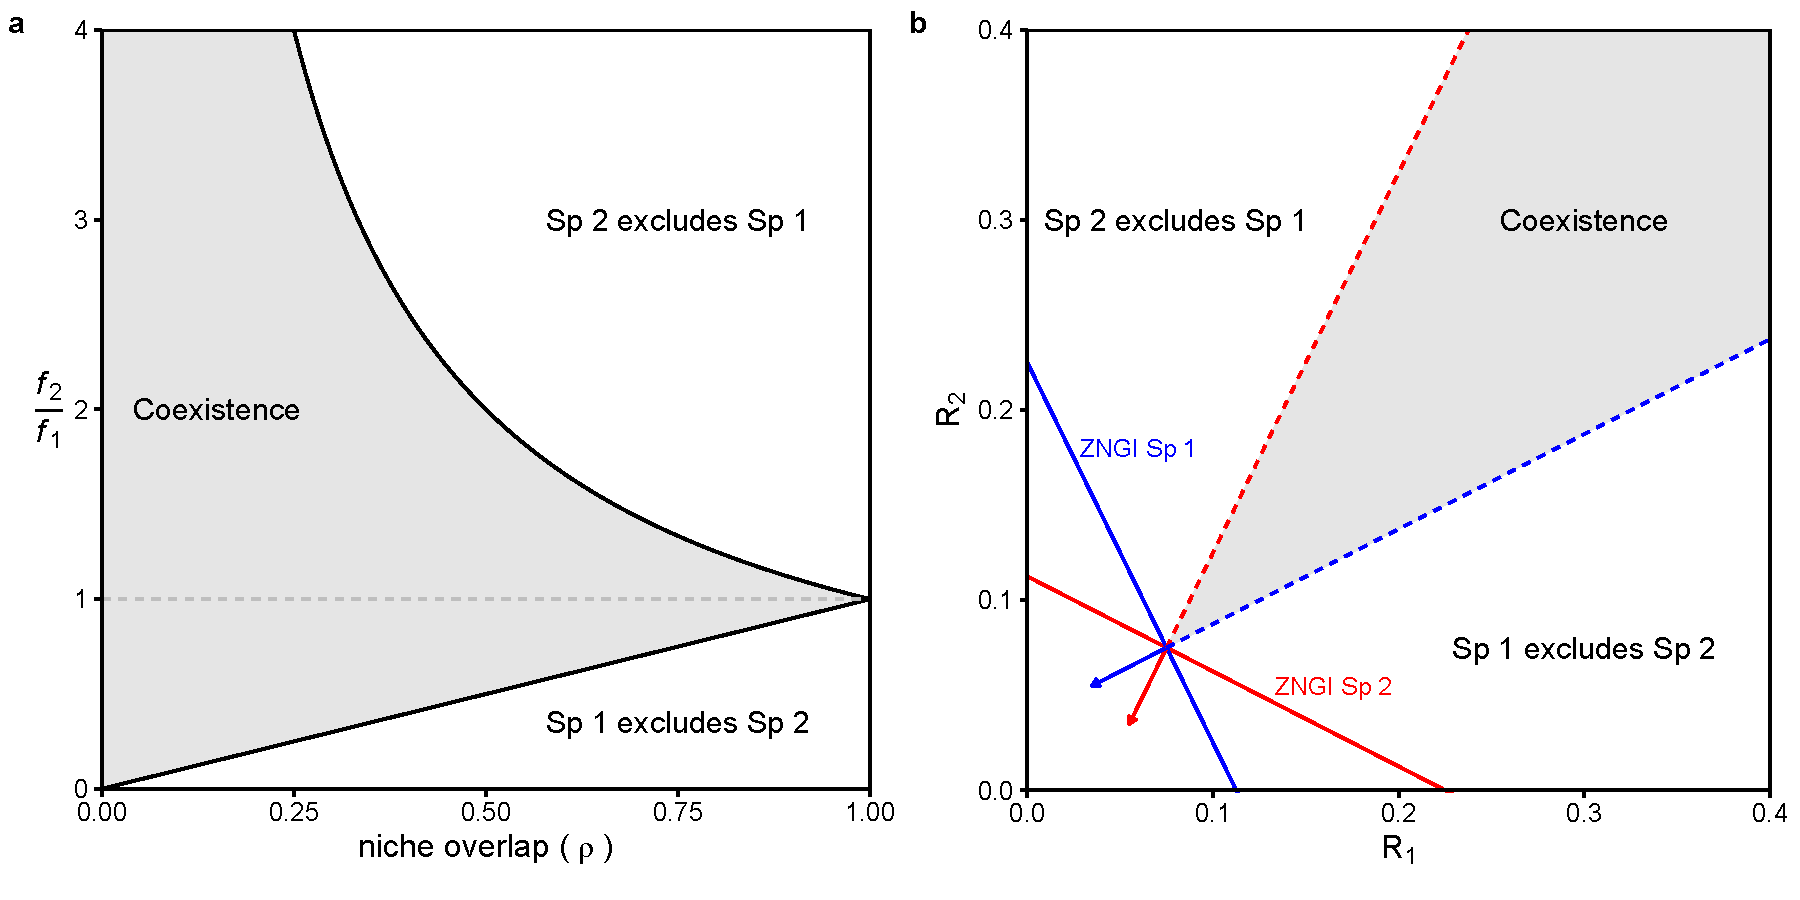
\includegraphics[width=15cm]{Chapter2/conceptfig.pdf}}
\caption[Graphical illustration of the criteria for coexistence under modern coexistence theory and contemporary niche theory.]
	{\hspace{1mm}Graphical illustration of the criteria for coexistence under modern coexistence theory (a) and contemporary niche theory (b). In (a) the lower and upper bounding black lines denote the point where the fitness ratio is equal to niche overlap and the inverse of niche overlap, respectively. Thus, according to the inequality $\rho < f_{2}/f_{1} < 1/\rho$, two species can coexist in the shaded region but exclude each other above or below these bounding lines. The asymmetry in (a) is due to the y-axis being a ratio, and therefore would appear symmetrical on a log scale i.e., contrary to their appearance on the ratio scale, the unshaded regions of parameter space corresponding to exclusion are equal in size for both species. In (b) coexistence of two species competing for two substitutable resources depends on three criteria: intersecting ZNGIs (solid red and blue lines connecting the x- and y-axes); each species having a greater impact on the resource from which it most benefits (impact vectors denoted by the red and blue arrows); and a resource supply ratio that is intermediate to the inverse of the impact vectors (dashed red and blue lines).}
\label{fig:conceptfig}
\end{figure}



\newpage
\begin{figure}[h!]
\centering
\makebox[\textwidth][c]{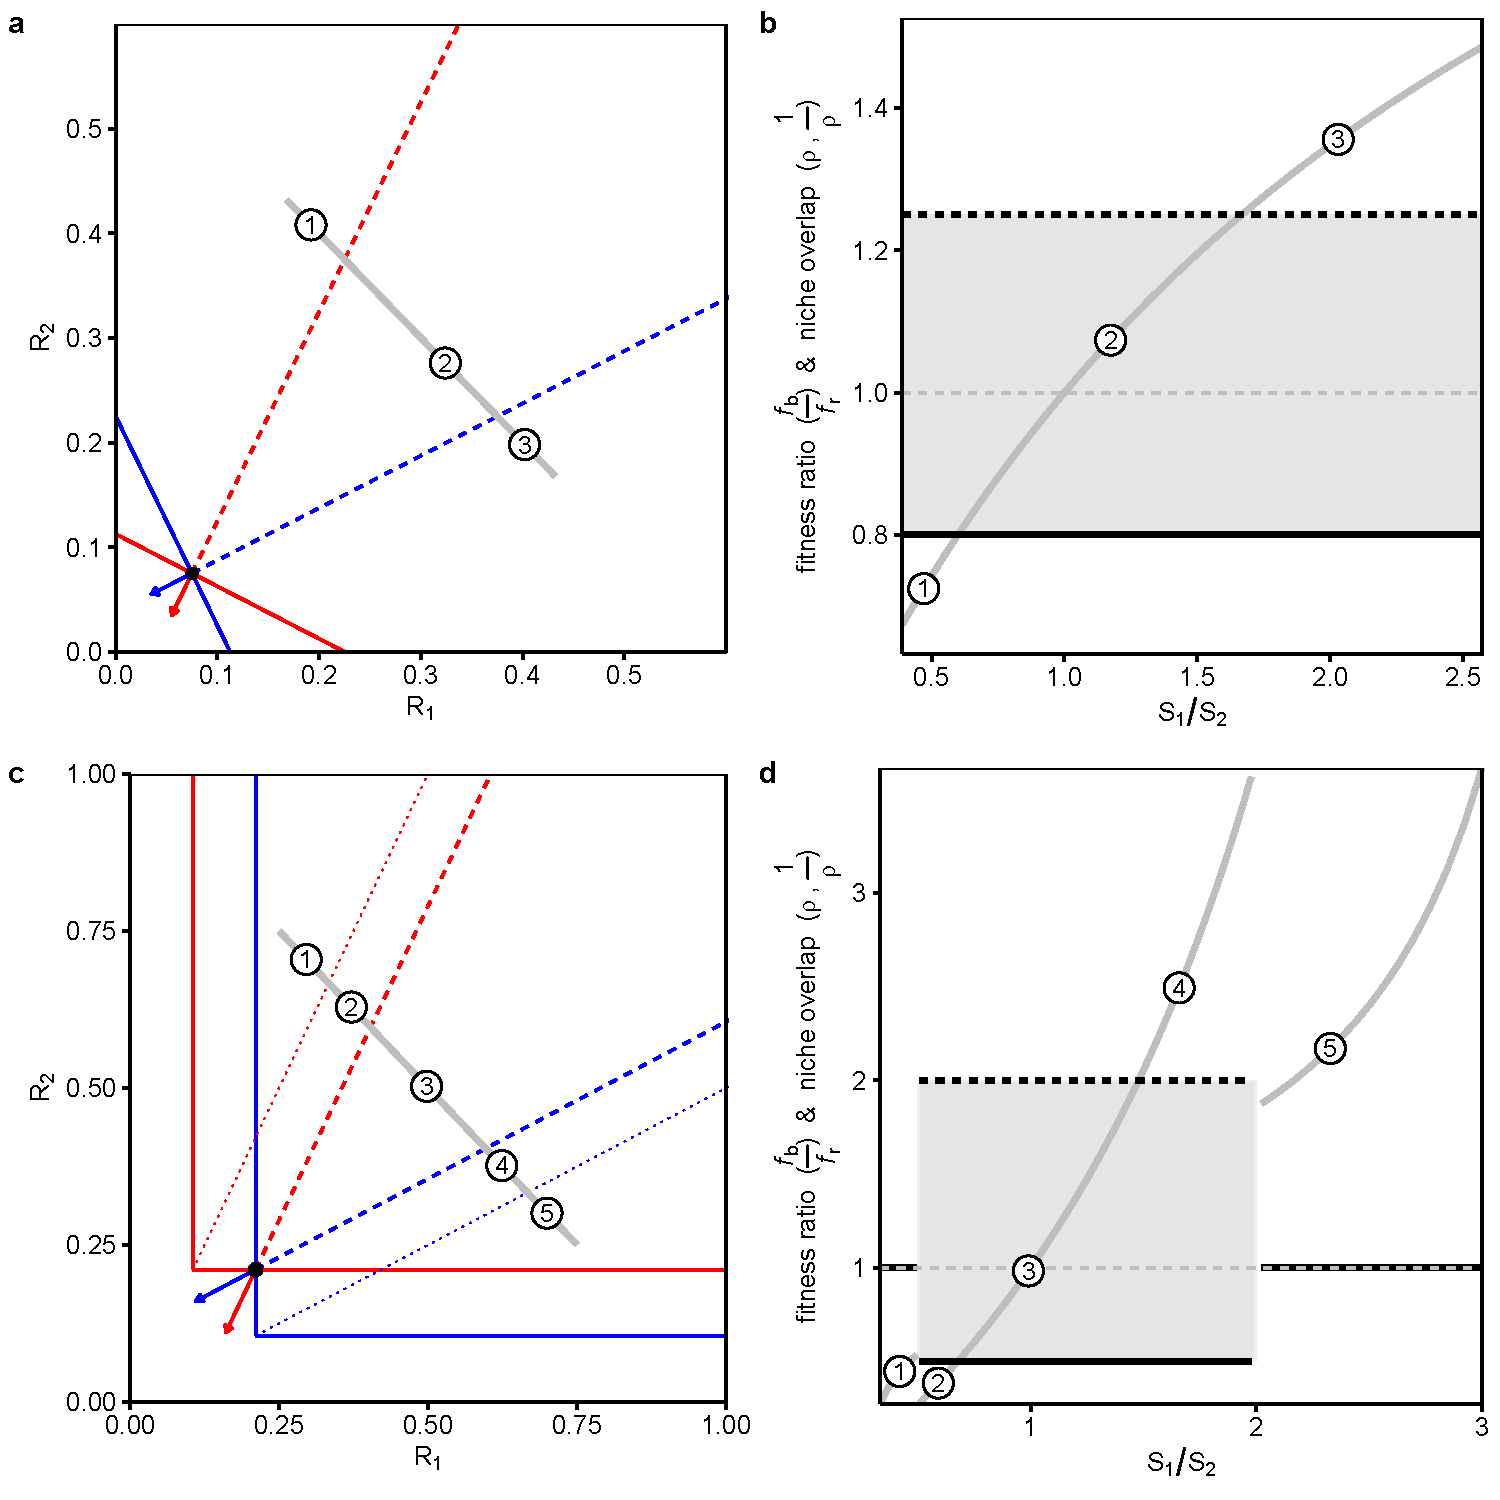
\includegraphics[width=12cm]{Chapter2/supply-ms-fig-flippedcols.pdf}}
\caption[Translating changing resource supply ratios in contemporary niche theory into the equalizing and stabilizing terms of modern coexistence theory, under pairwise competition for substitutable and essential resources.]
	{\hspace{1mm}Translating changing resource supply ratios in contemporary niche theory (a \& c) into the equalizing and stabilizing terms of modern coexistence theory (b \& d), under pairwise competition for substitutable (a \& b) and essential resources (c \& d). In (a) and (c), the solid red and blue lines are the ZNGIs for each species; the solid lines with arrow heads are the respective impact vectors; and the dashed lines are the inverse of the impact vectors, defining regions of stable coexistence. The additional dotted lines in (c) denote the regions in which species switch from being limited by different resources (above blue and below red) to being limited by the same resource (below blue or above red). In (b) and (d), the x-axis represents the resource ratio moving along the grey lines in (a) and (c) from top left to bottom right. The y-axis gives the values of the fitness ratio, $f_{b}/f_{r}$ (solid grey line), and the degree of niche overlap, $\rho$ (solid black line) and $1/\rho$ (dashed black line). The grey shaded area indicates the coexistence region, where $\rho<f_{b}/f_{r}<1/\rho$. For reference, equal fitness, where $f_{b}/f_{r}=1$, is illustrated by the horizontal dashed grey line. Numbers 1-3 in (a) and 1-5 in (c) correspond to the respective numbers in (b) and (d).}
\label{fig:supply-ms-fig}
\end{figure}



\newpage
\begin{figure}[h!]
\centering
\makebox[\textwidth][c]{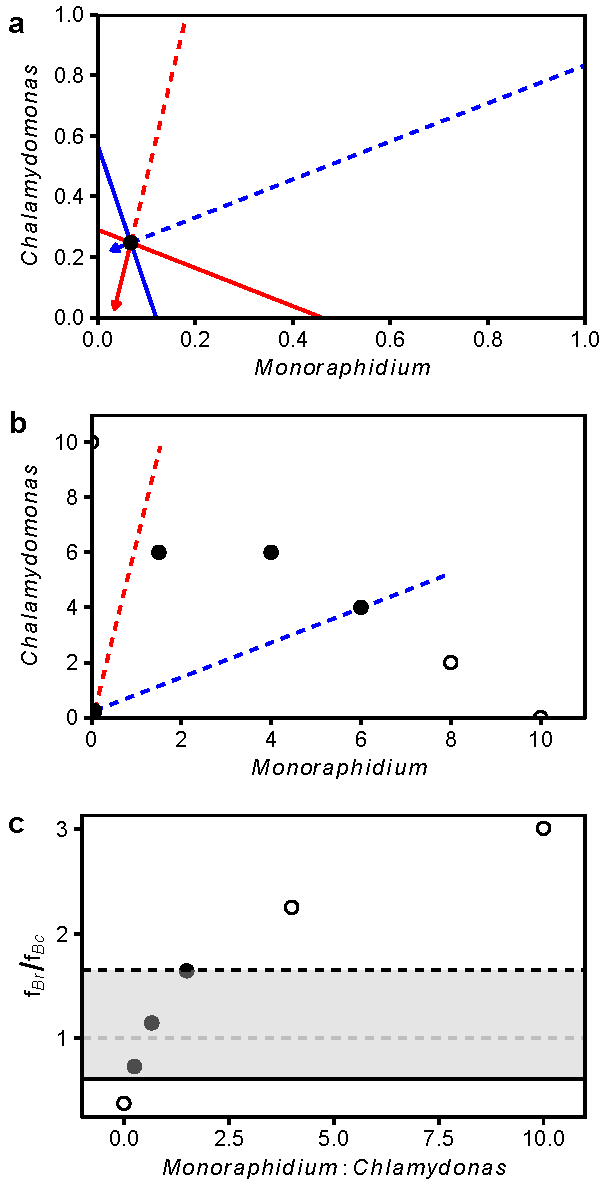
\includegraphics[width=7cm]{Chapter2/Box2-fig-Rothhaupt-colswitch.pdf}}
\caption[Illustrating the equivalence of predictions from contemporary niche theory and modern coexistence theory using data from \citet{Rothhaupt1988}.]
	{\hspace{1mm}Illustrating the equivalence of predictions from contemporary niche theory and modern coexistence theory using data from \citet{Rothhaupt1988}. In the top panel (a) ZNGIs and consumption vectors for \textit{B. rubens} and \textit{B. calyciflorus} are shown in blue and red respectively. The relationship between different supply point ratios (circles) and the inverse of the consumption vectors are shown in the middle panel (b), where filled circles indicate supply points where both species are predicted to coexist and empty circles indicate regions where one species is predicted to competitively exclude the other. The corresponding niche overlap, $\rho$, and fitness ratio, $f_{Br}/f_{Bc}$, values are shown in the bottom panel (c). Solid and dashed black lines indicate $\rho$ and $1/\rho$ respectively; dashed grey line indicates equal fitness; filled circles indicate regions of coexistence where  $\rho < f_{Br}/f_{Bc} < 1/\rho$; empty circles indicate regions of competitive exclusion.}
\label{fig:Box2-fig-Rothhaupt}
\end{figure}



\newpage
\begin{figure}[h!]
\centering
\makebox[\textwidth][c]{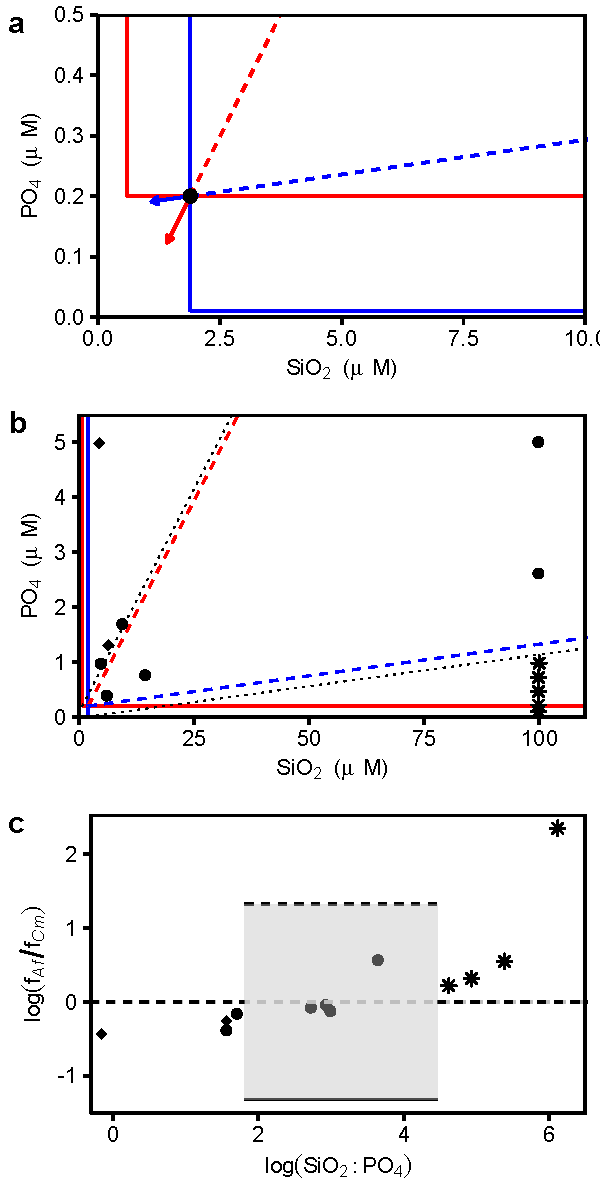
\includegraphics[width=7cm]{Chapter2/Box2-fig-Tilman-colswitch.pdf}}
\caption[Illustrating the equivalence of predictions from contemporary niche theory and modern coexistence theory using data from \citet{Tilman1977, tilman1982}.]
	{\hspace{1mm} Illustrating the equivalence of predictions from contemporary niche theory and modern coexistence theory using data from \citet{Tilman1977, tilman1982}. In the top panel (a) ZNGIs and consumption vectors for \textit{Asterionella} and \textit{Cyclotella}) are shown in blue and red respectively. The relationship between different supply point ratios and the inverse of the consumption vectors are shown in the middle panel (b). Corresponding with Fig. 31.A of \citet{tilman1982}, the supply point symbols indicate the outcome of competition experiments where stars denote the exclusion of \textit{Cyclotella} by \textit{Asterionella}, dots denote coexistence, and diamonds denote the exclusion of \textit{Asterionella} by \textit{Cyclotella}. The corresponding niche overlap, $\rho$, and fitness ratio, $f_{Af}/f_{Cm}$, values are shown in the bottom panel (c). Solid and dashed black lines indicate $\rho$ and $1/\rho$ respectively; dashed grey line indicates equal fitness; shaded area indicates region of coexistence where  $\rho < f_{Af}/f_{Cm} < 1/\rho$. To aid visualization, both axes in (c) have been log-transformed.}
\label{fig:Box2-fig-Tilman}
\end{figure}



\newpage
\begin{figure}[h!]
\centering
\makebox[\textwidth][c]{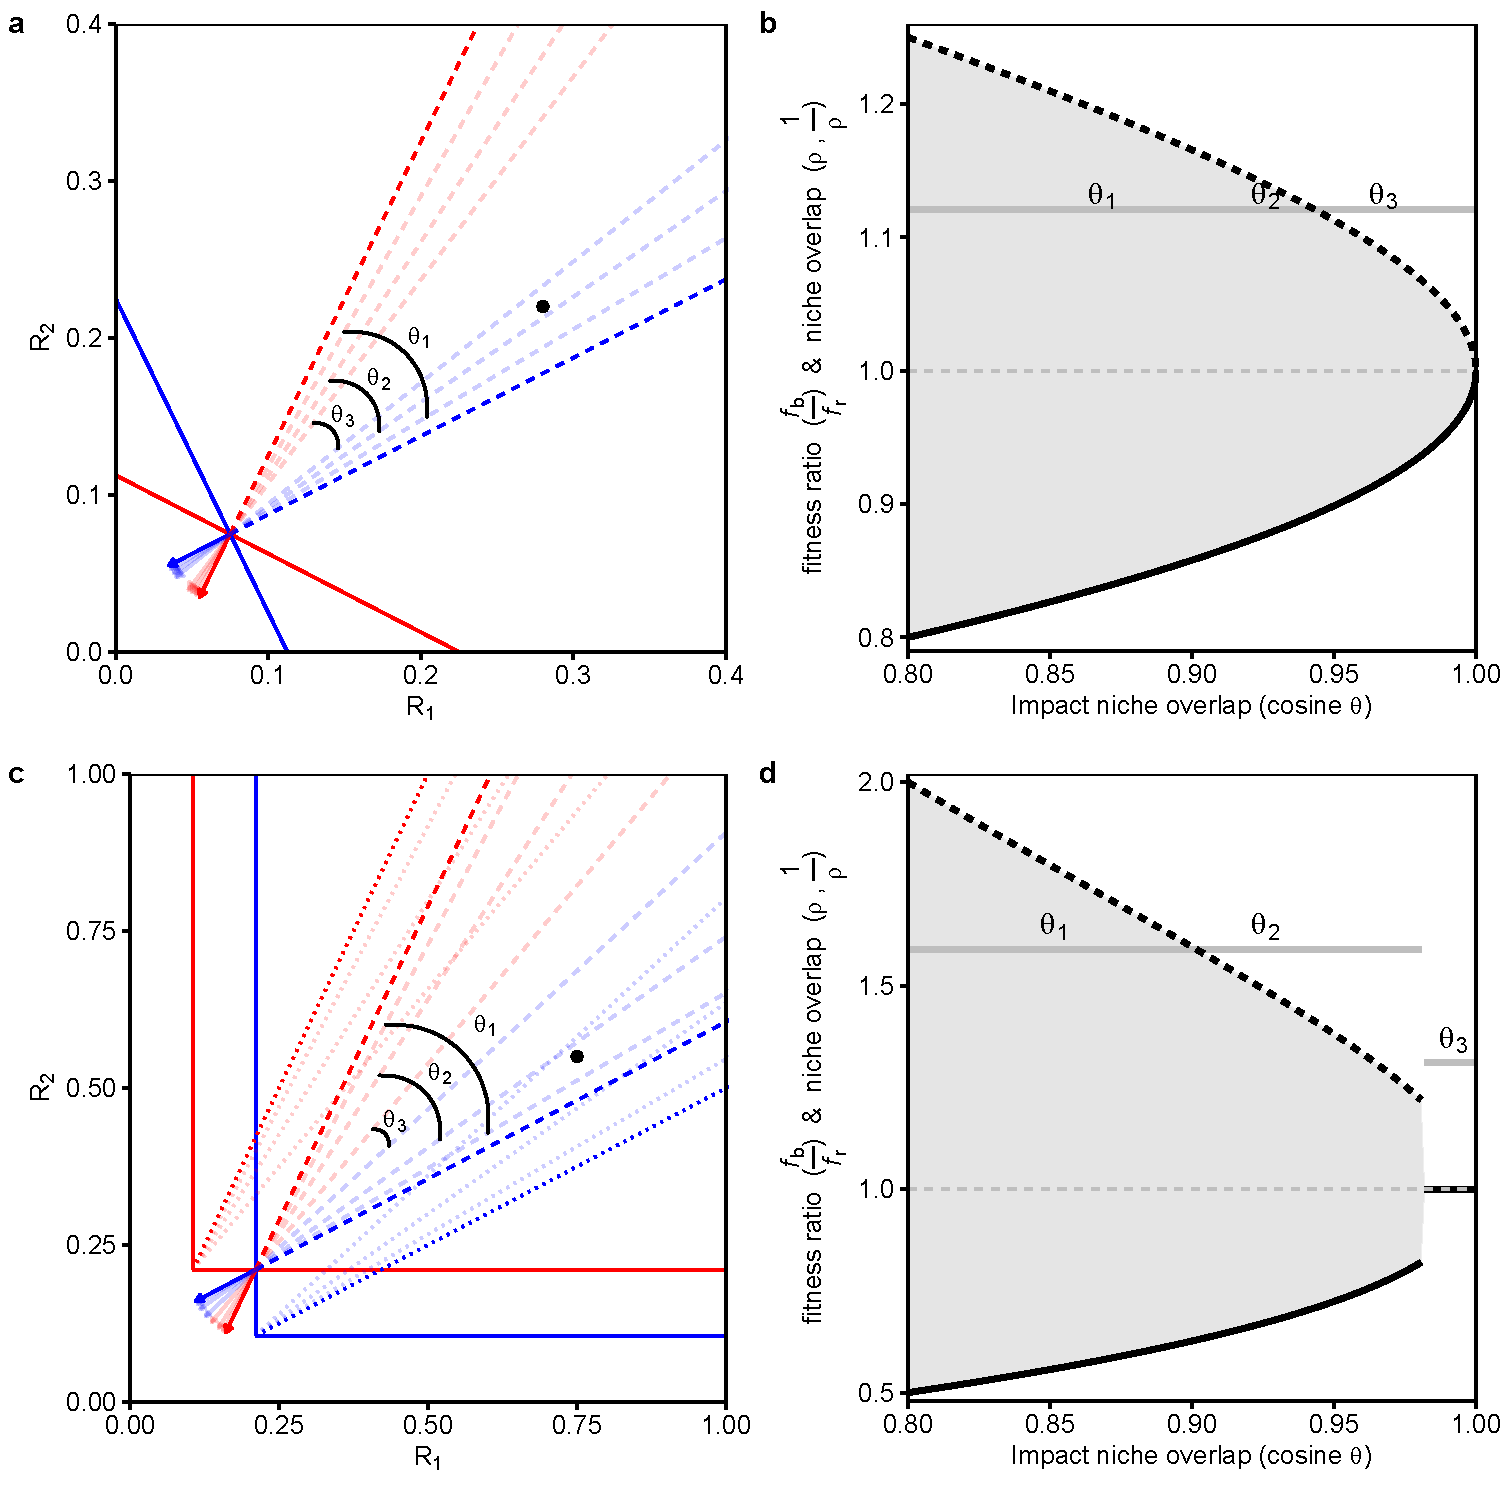
\includegraphics[width=12cm]{Chapter2/impact-ms-fig-flippedcols.pdf}}
\caption[Translating changing impact niche overlap in contemporary niche theory into the equalizing and stabilizing terms of modern coexistence theory, under pairwise competition for substitutable and essential resources.]
	{\hspace{1mm}Translating changing impact niche overlap in contemporary niche theory (a \& c) into the equalizing and stabilizing terms of modern coexistence theory (b \& d), under pairwise competition for substitutable (a \& b) and essential resources (c \& d). In (a) and (c), the solid red and blue lines are the ZNGIs for each species; the solid lines with arrow heads are the respective impact vectors; and the dashed lines are the inverse of the impact vectors, defining regions of stable coexistence. The additional dotted lines in (c) denote the regions in which species switch from being limited by different resources (above blue and below red) to being limited by the same resource (below blue or above red). In (b) and (d), the x-axis represents the impact niche overlap starting in the position given by the bold dashed lines and ending at complete overlap. The y-axis gives the values of the fitness ratio, $f_{b}/f_{r}$ (solid grey line), and the degree of niche overlap, $\rho$ (solid black line) and $1/\rho$ (dashed black line). The grey shaded area indicates the coexistence region, where $\rho<f_{b}/f_{r}<1/\rho$. For reference, equal fitness, where $f_{b}/f_{r}=1$, is illustrated by the horizontal dashed grey line. The angles given by $\theta_{1-3}$ in (a) and (c) correspond to the respective $\theta_{1-3}$ in (b) and (d). Impact niche overlap is defined here as the cosine of the angle between species' impact vectors, $\mathit{cosine}\ \theta = \nicefrac{\left( c_{11}c_{21}+c_{12}c_{22} \right)}{\left( \sqrt{c_{11}^{2}+c_{12}^{2}}\times \sqrt{c_{21}^{2}+c_{22}^{2}} \right)}$, where $\left (c_{i1}, c_{i2}\right )$ is the consumption vector for species $\mathit{i}$ (see Appendix A.1 and Box 1 for parameter definition).}
\label{fig:impact-ms-fig}
\end{figure}



\newpage
\begin{figure}[h!]
\centering
\makebox[\textwidth][c]{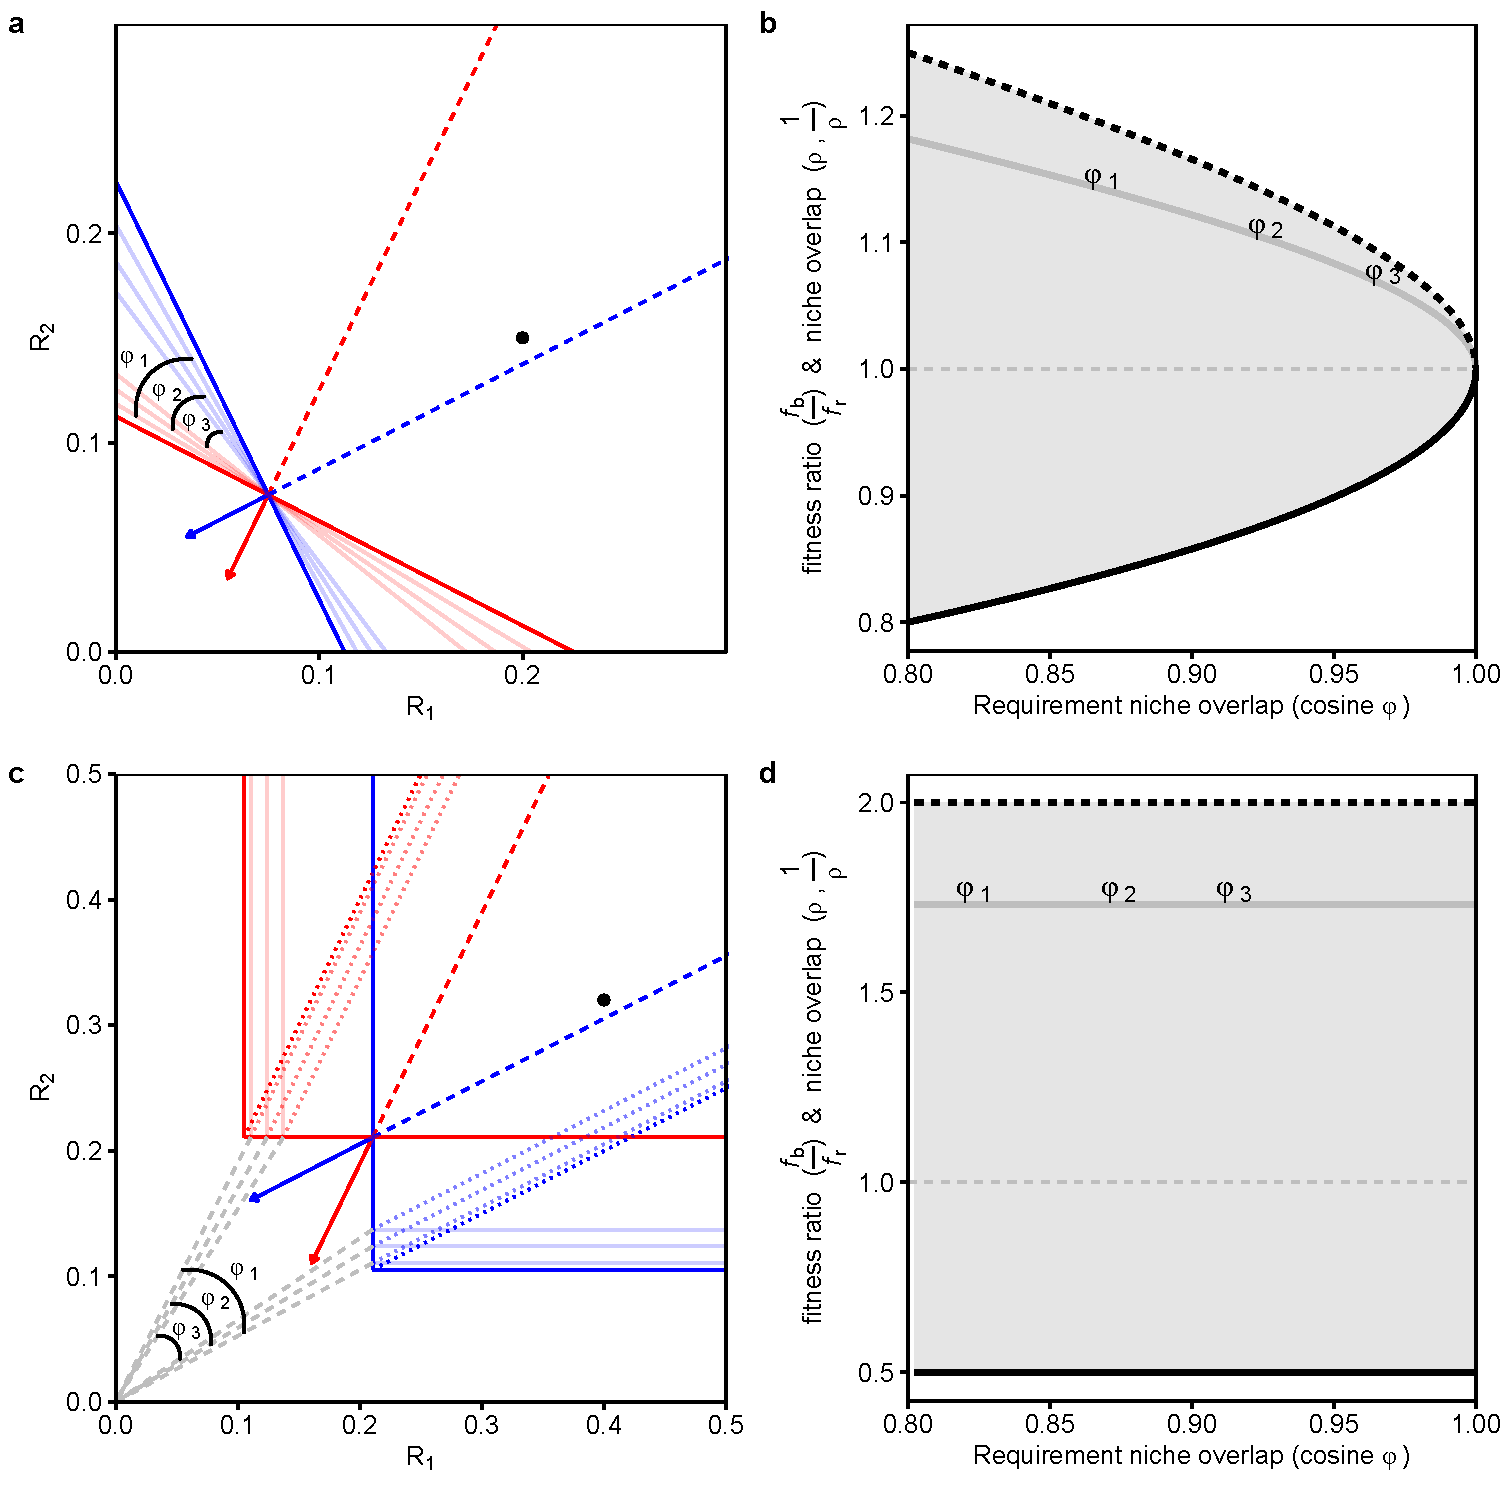
\includegraphics[width=12cm]{Chapter2/require-ms-fig-fixedequilibrium-flippedcols.pdf}}
\caption[Translating changing requirement niche overlap in contemporary niche theory into the equalizing and stabilizing terms of modern coexistence theory, under pairwise competition for substitutable and essential resources.]
	{\hspace{1mm}Translating changing requirement niche overlap in contemporary niche theory (a \& c) into the equalizing and stabilizing terms of modern coexistence theory (b \& d), under pairwise competition for substitutable (a \& b) and essential resources (c \& d). In (a) and (c), the solid red and blue lines are the ZNGIs for each species; the solid lines with arrow heads are the respective impact vectors; and the dashed lines are the inverse of the impact vectors, defining regions of stable coexistence. The additional dotted lines in (c) denote the regions in which species switch from being limited by different resources (above blue and below red) to being limited by the same resource (below blue or above red). In (b) and (d), the x-axis represents the requirement niche overlap starting in the position given by the solid bold ZNGIs and ending at complete overlap. The y-axis gives the values of the fitness ratio, $f_{b}/f_{r}$ (solid grey line), and the degree of niche overlap, $\rho$ (solid black line) and $1/\rho$ (dashed black line). The grey shaded area indicates the coexistence region, where $\rho<f_{b}/f_{r}<1/\rho$. For reference, equal fitness, where $f_{b}/f_{r}=1$, is illustrated by the horizontal dashed grey line. The angles given by $\varphi_{1-3}$ in (a) and (c) correspond to the respective $\varphi_{1-3}$ in (b) and (d). Requirement niche overlap for substitutable resources is defined here as the cosine of the angle between species' ZNGIs, $\mathit{cosine}\ \phi  = \nicefrac{\left( w_{12}w_{22}+w_{11}w_{21} \right)}{\left( \sqrt{w_{11}^{2}+w_{12}^{2}} \times \sqrt{w_{21}^{2}+w_{22}^{2}} \right)}$, where $\nicefrac{-w_{i1}}{w_{i2}}$ is the ZNGI's slope for species $\mathit{i}$. Requirement niche overlap for essential resources is defined as the cosine of the angle between two lines from the origin to the corner of each ZNGI, $\mathit{cosine}\ \phi  = \nicefrac{\left( R_{11}^{*}R_{21}^{*}+R_{12}^{*}R_{22}^{*} \right)}{\left( \sqrt{R_{11}^{*2}+R_{12}^{*2}}\times \sqrt{R_{21}^{*2}+R_{22}^{*2}} \right)}$, where $\left (R_{i1}^{*}, R_{i2}^{*}\right )$ represents the ZNGI's corner for species $\mathit{i}$ (see also main text, Appendix A.1 and Box 1).}
\label{fig:require-ms-fig-fixedequilibrium}
\end{figure}



\clearpage 
\begin{tcolorbox}[breakable, leftright skip=-0.5cm]
\subsection*{Box 1: Deriving niche overlap and fitness differences in terms of consumer-resource parameters}
In order to explore the analytical relationship between modern coexistence theory \citep{Chesson2000} and contemporary niche theory \citep{Chase2003} we first translated a consumer-resource model into Lotka--Volterra form following \citet[][Ch.~7]{tilman1982}. This was done by solving the equilibrium of the consumer-resource model, and rearranging the equilibrium algebraically \citep[for an alternative approach see][]{Meszenaz2006, Barabas2014}. A summary of the mathematical derivation for substitutable resources is provided here, and in full for both substitutable and essential resources in Appendix A.1.
\par


Tilman's (\citeyear{tilman1982}) consumer-resource model consists of two resources ($R_{1}$ and $R_{2}$) that are perfectly nutritionally substitutable for two consumers ($N_{1}$ and $N_{2}$). By setting the right hand side of the consumer equations to zero, \citet{tilman1982} solved for the equilibrium and rearranged the consumer equilibrium density to a form comparable to the Lotka--Volterra model (i.e., $N_{1}^{*}=\frac{1}{a_{11}}-\frac{a_{12}}{a_{11}}N_{2}^{*}$ and $N_{2}^{*}=\frac{1}{a_{22}}-\frac{a_{21}}{a_{22}}N_{1}^{*}$). The equilibrium density for $N_{1}$ and $N_{2}$ can be subsequently written as:

\begin{equation}
N_1^* = \left[ {\frac{{D\left( {{S_2} + \frac{{{w_{11}}}}{{{w_{12}}}}{S_1} - {B_1}} \right)}}{{{c_{12}} + {c_{11}}\frac{{{w_{11}}}}{{{w_{12}}}}}}} \right] - \left[ {\frac{{{c_{22}} + {c_{21}}\frac{{{w_{11}}}}{{{w_{12}}}}}}{{{c_{12}} + {c_{11}}\frac{{{w_{11}}}}{{{w_{12}}}}}}} \right]N_2^*
\tag{2.4.1}\label{eq:2.4.1}
\end{equation}
\begin{equation}
N_2^* = \left[ {\frac{{D\left( {{S_2} + \frac{{{w_{21}}}}{{{w_{22}}}}{S_1} - {B_2}} \right)}}{{{c_{22}} + {c_{21}}\frac{{{w_{21}}}}{{{w_{22}}}}}}} \right] - \left[ {\frac{{{c_{12}} + {c_{11}}\frac{{{w_{21}}}}{{{w_{22}}}}}}{{{c_{22}} + {c_{21}}\frac{{{w_{21}}}}{{{w_{22}}}}}}} \right]N_1^*.
\tag{2.4.2}\label{eq:2.4.2}
\end{equation}

\noindent Here, $r_{i}$ represents the maximum population growth rate for species $i$ ($i = $ 1 or 2) and $D$ represents the constant mortality of the consumers and turnover rate of resources. Per capita resource consumption rate of consumer $N_{i}$ on resource $R_{j}$ ($j = $ 1 or 2) is represented by $c_{ij}$, whereas $w_{ij}$ represents a weighting factor that converts availability of $R_{j}$ into its value for consumer $N_{i}$. Following a Monod growth model, $k_{i}$ is the half-saturation constant for $N_{i}$ resource consumption, and $T_{i}$ is the minimum amount of total resource required for $N_{i}$ to grow. Finally, $S_{1}$ and $S_{2}$ represents the resource supply concentration for $R_{1}$ and $R_{2}$, respectively.
\par


Eqns.~\ref{eq:2.4.1} and \ref{eq:2.4.2} consists of two parts. The first bracket represents a density-independent component with only $N_{1}$- and $N_{2}$-related parameters and are the algebraic equivalent of $\frac{1}{a_{11}}$ and $\frac{1}{a_{22}}$, respectively. The second bracket represents a heterospecific density-dependent component that decreases with its competitors' density, and is the algebraic equivalent of $\frac{a_{12}}{a_{11}}$ and $\frac{a_{21}}{a_{22}}$ in the Lotka--Volterra model, respectively.
\par


Chesson defines niche overlap as $\rho=\sqrt {\frac{{{a_{12}}{a_{21}}}}{{{a_{11}}{a_{22}}}}}$ and average fitness difference of $N_{2}$ over $N_{1}$ as $\frac{{{f_2}}}{{{f_1}}} = \sqrt {\frac{{{a_{11}}{a_{12}}}}{{{a_{22}}{a_{21}}}}}$ \citep{Chesson2008b, Chesson2013ecosys}. Thus niche overlap for two consumers competing for substitutable resources can be expressed as:

\begin{equation}
\rho  = \sqrt {\frac{{{a_{12}}{a_{21}}}}{{{a_{11}}{a_{22}}}}}  = \sqrt {\frac{\left (
		c_{22} + c_{21}\frac{w_{11}}{w_{12}}\right )\left ( 
		c_{12} + c_{11}\frac{w_{21}}{w_{22}} \right )}{\left (
		c_{12} + c_{11}\frac{w_{11}}{w_{12}}\right )\left ( 
		c_{22} + c_{21}\frac{w_{21}}{w_{22}} \right )}} 
\tag{2.5.1}\label{eq:2.5.1}
\end{equation}
and the absolute fitness difference of $N_{2}$ over $N_{1}$ is:
\begin{equation}
\frac{{{f_2}}}{{{f_1}}} = \sqrt {\frac{{{a_{11}}{a_{12}}}}{{{a_{22}}{a_{21}}}}}  = \frac{\left (S_{2}+\frac{w_{21}}{w_{22}}S_{1}-B_{2}\right )}{\left (S_{2}+\frac{w_{11}}{w_{12}}S_{1}-B_{1}\right )}\sqrt {\frac{\left (
		c_{12} + c_{11}\frac{w_{11}}{w_{12}}\right )\left ( 
		c_{22} + c_{21}\frac{w_{11}}{w_{12}} \right )}{\left (
		c_{22} + c_{21}\frac{w_{21}}{w_{22}}\right )\left ( 
		c_{12} + c_{11}\frac{w_{21}}{w_{22}} \right )}}.
\tag{2.5.2}\label{eq:2.5.2}
\end{equation}
\end{tcolorbox}



\clearpage
\begin{tcolorbox}[breakable, leftright skip=-0.5cm]
\subsubsection*{Box 2: Empirical tests of consumer-resource competition through the lens of modern coexistence theory}
In order to illustrate further the transformation between contemporary niche theory and modern coexistence theory, we extracted data from two seminal experimental works on resource competition, \citet{Rothhaupt1988} and \citet{Tilman1977}. 
\par


\citet{Rothhaupt1988} investigated the effect of modifying the ratio of two substitutable resources on the competitive dynamics of two species of herbivorous zooplankton, the rotifers \textit{Brachionus rubens} and \textit{B. calyciflorus}. To quantity the parameters defining each species' ZNGI and consumption vectors, \citet{Rothhaupt1988} first measured the per capita growth rate of \textit{B. rubens} and \textit{B. calyciflorus} across a range of concentrations of two algae species (\textit{Monoraphidium minutum} and \textit{Chlamydonas sphaeroides}). These were subsequently used to make predictions on the outcomes of competition between the two rotifers at different supply ratios of the two resources and at two dilution rates (the nutrient independent mortality rate in a chemostat).
\par


We extracted the relevant parameters at the lower dilution rate (either from the text or from figure 2a) and used these to quantify Chesson's niche overlap and fitness ratio terms following the approach outlined in Box 1. Fig.~\ref{fig:Box2-fig-Rothhaupt}a shows each species' ZNGI and associated consumption vector, and corresponds with Figure 2a of \citet{Rothhaupt1988}. Notably the intersecting ZNGIs and positively correlated consumption vectors satisfy two of the three criteria for stable coexistence. Fig. \ref{fig:Box2-fig-Rothhaupt}b, which is drawn on a different scale to Fig. \ref{fig:Box2-fig-Rothhaupt}a, shows the manipulated resource supply ratios, where black dots satisfy the third criteria for stable coexistence, intermediate supply rates. Fig. \ref{fig:Box2-fig-Rothhaupt}c shows the equivalent coexistence predictions when translated into Chesson's niche overlap and fitness ratio. In accordance with the logic of the main text, manipulating resource supply ratio only affects fitness differences, and the regions of stable coexistence correspond with those identified by Tilman's graphical method. In subsequent competition experiments, \citet{Rothhaupt1988} found the results to be in agreement with theoretical predictions in all but one of the scenarios outlined above.
\par


Tilman (\citeyear{Tilman1977, tilman1982}) investigated the effect of modifying the ratios of two essential resources, phosphate and silicate, on the coexistence of two algal species, \textit{Asterionella formosa} and \textit{Cyclotella meneghiniana}. As for the Rothhaupt data, we used the parameters given in \cite{Tilman1977} and extracted the supply point ratios from Fig. 31.A of \citet{tilman1982} to quantify Chesson's niche overlap and fitness ratio terms. Fig. \ref{fig:Box2-fig-Tilman}a shows a zoomed-in view of each species' ZNGIs and impact vectors. Fig. \ref{fig:Box2-fig-Tilman}b, which corresponds with Fig. 31.A of \citet{tilman1982}, shows the position of the resource supply points and predicted outcomes of competition. When translated into Chesson's niche overlap and fitness ratio terms (Fig. \ref{fig:Box2-fig-Tilman}c) we see that the four supply points compatible with coexistence in Fig. \ref{fig:Box2-fig-Tilman}b all correspond with fitness ratios that are bounded by $\rho$ \& $1/\rho$. As highlighted in the main text, all of the supply points that fall outside the coexistence region are sufficiently extreme such that both species are limited by the same resource. This is reflected in the superimposition of $1/\rho$ and $\rho$ in Fig. \ref{fig:Box2-fig-Tilman}c. The results of subsequent competition experiments were in agreement with all but two of the predictions, where both species coexisted despite falling just outside the coexistence region identified in Fig. \ref{fig:Box2-fig-Tilman}b.
\par


Note that the equivalence of the coexistence predictions in both examples is a natural result of their deriving from the same underlying data. It would be valuable to conduct a more thorough comparative study using data collected independently for analysis under each framework, where inconsistent predictions could serve to highlight inappropriate assumptions.
\end{tcolorbox}

\chapter{Coexistence theory and the frequency-dependence of priority effects}
%\chaptermark{Positive frequency-dependence}
%\renewcommand{\sectionmark}[1]{}
\fancyhead[LE, RO]{\thepage}
\fancyhead[RE]{CHAPTER 3}
\fancyhead[LO]{POSITIVE FREQUENCY-DEPENDENCE}
\fancyfoot{}
\renewcommand{\headrulewidth}{0pt}
\setlength{\parindent}{1cm}


\begin{comment}
\documentclass[hidelinks,12pt]{article}
\usepackage{graphicx,bm, booktabs,lineno,array}
\usepackage[fleqn]{amsmath}
\setlength{\mathindent}{0pt}
\usepackage[super,comma,numbers, compress]{natbib}
\usepackage[a4paper]{geometry}
\usepackage[parfill]{parskip}
\usepackage[usenames,dvipsnames]{color}
\usepackage[font=footnotesize,labelfont=bf,margin=1cm, labelsep = none]{caption} 
\usepackage{setspace}
\usepackage{gensymb}
\usepackage{color} 
\usepackage{sidecap}
\usepackage{epigraph}
\usepackage{float}
\usepackage{soul,xcolor}
\setstcolor{red}
\setlength\epigraphwidth{12cm}
\setlength\epigraphrule{0pt}
\usepackage{etoolbox}
\usepackage{tcolorbox}
\tcbuselibrary{breakable}
\usepackage[bottom, symbol]{footmisc}
\usepackage{authblk}
\usepackage{hyperref}
\usepackage[color=cyan]{todonotes}
\pdfminorversion=3
\doublespacing

\renewcommand{\epigraphflush}{center}
\renewcommand{\sourceflush}{flushleft}
\newcommand{\plus}{\raisebox{.4\height}{\scalebox{.6}{+}}}
\newcommand{\minus}{\raisebox{.4\height}{\scalebox{.8}{-}}}
\renewcommand{\thefootnote}{\fnsymbol{footnote}}
\newcommand*\samethanks[1][\value{footnote}]{\footnotemark[#1]}
\newcommand\blfootnote[1]{%
  \begingroup
  \renewcommand\thefootnote{}\footnote{#1}%
  \addtocounter{footnote}{-1}%
  \endgroup
}
\end{comment}



\begin{comment}
\title{Coexistence theory and the frequency-dependence of priority effects}
\author[1]{Po-Ju Ke \thanks{Both authors contributed equally.}}
\author[1,2,3]{Andrew D. Letten \samethanks}
\affil[1]{Department of Biology, Stanford University, Stanford, California, 94305-5020, USA}
\affil[2]{Centre for Integrative Ecology, University of Canterbury, Christchurch, New Zealand}
\affil[3]{Institute of Integrative Biology, Department of Environmental Systems Science, ETH Z{\"u}rich, 8092 Z{\"u}rich, Switzerland}

\begin{document}

\date{}
\maketitle
\blfootnote{Correspondence email: pojuke@stanford.edu, andrew.letten@usys.ethz.ch}
%\textbf{Running title:} PFD
%\textbf{Keywords:} No key words for Forum 
\textbf{Type of article:} Brief Communication\\
\textbf{Number of words:} 1847 [main text] \\
\textbf{References:} 17\\
\textbf{Display items:} 3\\
\end{comment}



\section{Abstract}
Priority effects are commonly invoked to describe a broad suite of phenomena capturing the influence of species arrival order on the diversity, composition and function of ecological communities. Several studies have suggested reframing priority effects around the stabilizing and equalizing concepts of coexistence theory. We show that the only compatible priority effects are those characterized by positive frequency dependence, irrespective of whether they emerge in equilibrium or non-equilibrium systems. 



\section{Main text}
The order in which species arrive in a locality can have lasting impacts on the diversity, composition and function of ecological communities \citep{Chase2003Oecologia, Fukami2015}. This phenomenon, frequently referred to as priority effects, historical contingency or founder control \citep{Slatkin1974}, was originally explored analytically through Lotka--Volterra competition models \citep{Lewontin1969, May1971}. In these simple models, priority effects emerge when each species' growth rate is a positive function of its relative abundance, which results in the emergence of alternative stable states (panel a of Fig.~\ref{fig:FigBox}). From a theoretical perspective, the term priority effect is indeed synonymous with any process generating alternative stable states \citep{Petraitis2013}, but over time its usage has broadened to encompass a wider suite of phenomena, including those lacking multiple attractors. Several studies have subsequently mooted the prospect of reorganizing priority effects around the stabilizing and equalizing concepts of coexistence theory \citep{Mordecai2011, Fukami2016, Letten2017}. Here, we identify the unrecognized problems and promise of such an endeavour. In particular, we demonstrate that the only compatible priority effects are those characterized by positive frequency dependence. 
\par 


According to coexistence theory, species can coexist when the fitness differences between them are smaller than their niche differences, where the former compares overall adaptedness to a shared environment, and the latter captures overlap in resource usage in space and time \citep{Chesson2000}. This is equivalent to stating that each species exhibits negative frequency dependence (NFD); i.e., reduced growth as a function of its own relative abundance in a community. For a two-species Lotka--Volterra competition model, this can be summarized via the inequality 

\begin{equation}
\rho < \frac{f_{2}}{f_{1}} < 1/\rho
\tag{3.1}\label{eq:3.1}
\end{equation}

\noindent where niche overlap, $\rho$, is equal to `1 - the niche difference' and is bounded between 0 and 1, and $\frac{f_{2}}{f_{1}}$ is the fitness ratio (panel b, c of Fig.~\ref{fig:FigBox}). It follows that we can differentiate between two classes of coexistence mechanisms: equalizing mechanisms that reduce the fitness difference and stabilizing mechanisms that reduce niche overlap. 
\par


In addition to being ecologically intuitive, the bounding of niche overlap between 0 and 1 has statistical provenance in Chesson's original definition as the correlation between species' resource utilization functions in MacArthur's consumer-resource model \citep{Chesson1990}. More recently, however, Chesson provided a convenient formula for niche overlap in terms of the Lotka--Volterra competition coefficients, $\alpha_{ij}$ \citep{Chesson2013ecosys}. Specifically,

\begin{equation}
\rho=\sqrt {\frac{{{\alpha_{12}}{\alpha_{21}}}}{{{\alpha_{11}}{\alpha_{22}}}}}.
\tag{3.2}\label{eq:3.2}
\end{equation}
 
\noindent Whether or not a given $\rho$ generates NFD depends on the fitness difference between competing species, but it is clear from this formulation that $\rho$ is bounded by 0 and 1 only when the product of the intra-specific coefficients is greater than the product of the inter-specific coefficients. When the reverse is true, $\rho$ takes values greater than 1, and the system exhibits priority effects giving rise to two alternative stable states, depending on species' initial density (panel a, b of Fig.~\ref{fig:FigBox}). 
\par


At first glance, $\rho>1$ is at odds with both intuitive and statistical interpretations of niche overlap, and seemingly becomes even more nonsensical when cast as a negative niche difference (1 - $\rho$). However, this break with convention operationalizes the criteria for positive frequency dependence (PFD), i.e., the analytical definition of priority effects, as the inverse of the stable coexistence inequality (panel b of Fig.~\ref{fig:FigBox}): 

\begin{equation}
\rho > \frac{f_{2}}{f_{1}} > 1/\rho.
\tag{3.3}\label{eq:3.3}
\end{equation}

\noindent Now, if we rename the niche difference ($1-\rho$) as the stabilization potential to avoid the semantic challenges of referring to a negative niche difference, we see from Eqn.~\ref{eq:3.3} that any mechanism that reduces the fitness ratio, or further decreases the stabilization potential below zero (i.e., further increases $\rho$ above one), will increase the probability of priority effects. Thus, like stable coexistence, we recognize that stable priority effects are also jointly controlled by both stabilizing and equalizing mechanisms. Note that the stabilization potential diverges around zero such that values above zero represent the stabilization potential for coexistence, whereas values below zero represent the stabilization potential for priority effects; in other words the strength of the attractor towards alternative stable states (panel b of Fig.~\ref{fig:FigBox}). Our terminology is different from recent heuristic translations of priority effects into coexistence theory, where the decrease of niche differences (i.e., stabilization potential) below zero has been referred to as destabilization \citep{Mordecai2011, Fukami2016}. However, while the coexistence attractor becomes unstable, multiple community attractors arise to be dynamically stable. Therefore, we favor conceptualizing destabilization as any process that causes the stabilization potential to approach zero from values above \textit{or} below (Fig. 1e). 
\par
 
 
A classic example of priority effects emerging from PFD comes from Tilman's 1982 monograph \cite{tilman1982}. Using the approach taken by Letten \textit{et al}.\cite{Letten2017} to derive niche overlap and the fitness ratio from Tilman's consumer-resource model, PFD generated priority effects can be partitioned into stabilizing and equalizing components. This partitioning is achieved by translating Tilman's model into a Lotka--Volterra form, which allows for the derivation of competition coefficients in terms of consumer-resource parameters. From there we can explore the effect of modifying mechanistic parameters on the stabilization potential using Eqn.~\ref{eq:3.2}, and the fitness ratio using the companion formula \citep{Chesson2008b, Chesson2013ecosys} (full derivation provided in Appendix B):

\begin{equation}
\frac{f_{2}}{f_{1}}=\sqrt {\frac{{{a_{11}}{a_{12}}}}{{{a_{22}}{a_{21}}}}}.
\tag{3.4}\label{eq:3.4}
\end{equation}

\noindent In Figure 1a, NFD and coexistence arise due to a combination of: 1) intersecting zero net growth isoclines (ZNGIs)\footnote{Zero net growth isocline (ZNGI) = the set of resource concentrations at which species' growth balances mortality. Consumption vectors = relative rates at which resources are depleted via consumption. Resource supply point = resource availability the system would return to in the absence of consumption.} indicating a trade-off in the two species competitive fitness for two substitutable resources where the red species benefits more from $R_{2}$ and the blue species from $R_{1}$; 2) consumption vectors that are directed towards each species' favored resource, such that the red species consumes more of $R_{2}$ and vice-versa, which is a prerequisite for intra-specific feedbacks being greater than inter-specific feedbacks; and 3) an intermediate resource ratio, which ensures neither species is overly advantaged by an imbalanced abundance of their favoured resource \citep{Chase2003, Letten2017}. As the angle between the consumption vectors declines to $\theta_{2}$ (Fig. 1b), the stabilization potential also declines. The outcome is competitive exclusion when the stabilization potential falls below the fitness ratio (Fig. 1e). Once the consumption vectors cross and begin to diverge, each species consumes more of its competitor's favored resource ($\theta_{3}$, Fig. 1c), setting up the conditions for PFD. However, if the fitness difference remains sufficiently large, the outcome will still be exclusion irrespective of arrival order (Fig. 1e). If the resource supply shifts to a more balanced ratio (Fig. 1d), the fitness inequality is reduced and priority effects emerge (Fig. 1e). The species that arrives first reduces the resource level of its competitors favoured resource below the competitor's $R^*$ - the minimum resource concentration required to maintain a positive growth rate, denoted by the intercept of the ZNGI with the resource axis. The result is that the late arriving competitor is unable to invade. 
\par


The above results demonstrate that priority effects are a function of both the stabilization potential and the fitness inequality, and that only a subset of phenomena commonly referred to as priority effects are compatible with coexistence theory. In particular, compatible phenomena are limited to those that generate PFD and therefore are consistent with the original definition derived from Lotka--Volterra \citep{Petraitis2013}. This is not to say that PFD is unique to systems exhibiting point equilibria. For example, the coexistence-affecting mechanism relative nonlinearity can generate PFD when species that benefit from fluctuations in the intensity of competition also exacerbate those fluctuations \citep{Chesson2009}. In Figure 2, two species with nonlinear functional responses exhibit negative average invader growth rates when competing for a logistically growing resource. As the resident, blue is able to draw resource levels below red's $R^*$ and therefore prevent red from invading, whereas, at sufficiently high initial density, red generates large resource fluctuations which blue is unable to control. Nevertheless, in a system that precludes the emergence of positive (or negative) frequency dependence, and hence the emergence of a non-zero stable attractor, the stabilization potential term is unquantifiable. This criterion, however, wholly or partially excludes a number of phenomena lacking multiple attractors, which for heuristic reasons are often included under the umbrella of priority effects (see examples in Fukami \cite{Fukami2015}). We briefly consider two of these phenomena below. 
\par


%\subsection*{Positive density dependence and facilitation}
When applying coexistence theory to study priority effects, it is important to recognize that PFD can emerge from negative or positive density dependence, i.e., facilitation. However, while Eqn.~\ref{eq:3.2}) cannot be leveraged to interpret the facilitative dynamics since negative $\alpha_{ij}$ in the Lotka--Volterra framework would generate unbounded population densities. Facilitation, of course, cannot go on forever and coexistence theory may still provide insight when negative density dependence starts to operate \citep{Schreiber2017}. However, unless constrained by specific model designs, the formulas can only be applied to PFD emerging from negative density dependence. 
\par


An alternative form of positive density dependence sometimes characterized as a priority effects is an Allee effect \citep{Petraitis2013}. For species exhibiting an Allee effect, there is a density threshold dividing two alternative stable states, i.e., above which the population persists and below which the population goes extinct. As such the alternative stable states arise from endogenous mechanisms at the population level, and therefore are distinct from priority effects that emerge at the community level driven by species interactions. Thus, while Allee effects can effect community composition if inter-specific interactions maintain species below their Allee threshold, they arise independently of a species' frequency in a community. 
\par


%\subsection*{Succession and transient priority effects}
Finally, the notion of priority effects has also been usefully applied to understand the effects of arrival order on successional dynamics. In these instances, differences in initial abundance can cause compositional trajectories to vary through time, even though they may all eventually converge on the same community state. Such ``alternative transient states" \citep{FukamiNakajima2011} can also be observed in naturally ephemeral microbial systems, such as those that develop in floral nectar or woody debris, where the final state might be the local extinction of all community members following the exhaustion of available resources. The trajectories of these communities, which are an outcome of resource pre-emption, may have downstream impacts on pollinator preference and decomposition rates and therefore undoubtedly reflect ecological phenomena with meaningful consequences for ecosystem function. Furthermore, it may well be relevant to consider these processes with respect to stabilizing mechanisms operating at some larger temporal or spatial scales. Nevertheless, treated independently of their broader spatio-temporal context, there is little scope or rationale to bring coexistence theory to bear on such phenomena. 
\par


%\subsection*{Summary}
Interest in coexistence theory has been growing steadily, but to date the overwhelming emphasis has been on the underlying stabilizing mechanisms giving rise to NFD and stable coexistence. We have illustrated the most accessible approach to incorporating priority effects mediated through PFD into this body of theory. When priority effects emerge from positive density dependence, or arise in transient systems, it is currently unclear how to analytically connect them to coexistence theory. 
\par



\section{Methods}
\subsection{Positive frequency dependence in an equilibrium system}
We first provide an example of positive frequency dependence (PFD) emerging from resource competition in an equilibrium system (Fig. 1). To this end, we take Tilman's original consumer-resource model \citep[p.~270]{tilman1982}, where two consumers (i.e. $N_{1}$ and $N_{2}$) are competing for two perfectly substitutable resources, $R_{1}$ and $R_{2}$. The dynamics of this system can be described as follows:

\begin{equation}
\frac{{d{N_1}}}{{dt}} = {r_1}{N_1}\left[ {\frac{{{w_{11}}{R_1} + {w_{12}}{R_2} - {T_1}}}{{{k_1} + {w_{11}}{R_1} + {w_{12}}{R_2} - {T_1}}}} \right] - D{N_1} \tag{3.7}\label{eq:3.7}
\end{equation}
\begin{equation}
\frac{{d{N_2}}}{{dt}} = {r_2}{N_2}\left[ {\frac{{{w_{21}}{R_1} + {w_{22}}{R_2} - {T_2}}}{{{k_2} + {w_{21}}{R_1} + {w_{22}}{R_2} - {T_2}}}} \right] - D{N_2} \tag{3.8}\label{eq:3.8}
\end{equation}
\begin{equation}
\frac{{d{R_1}}}{{dt}} = D\left( {{S_1} - {R_1}} \right) - {c_{11}}{N_1} - {c_{21}}{N_2} \tag{3.9}\label{eq:3.9}
\end{equation}
\begin{equation}
\frac{{d{R_2}}}{{dt}} = D\left( {{S_2} - {R_2}} \right) - {c_{12}}{N_1} - {c_{22}}{N_2} \tag{3.10}\label{eq:3.10}
\end{equation}

Here, $r_{i}$ represents the maximum population growth rate for species $i$ ($i = $ 1 or 2) and $D$ represents the constant mortality of the consumers and turnover rate of resources. Per capita resource consumption rate of consumer $N_{i}$ on resource $R_{j}$ ($j = $ 1 or 2) is represented by $c_{ij}$, whereas $w_{ij}$ represents a weighting factor that converts availability of $R_{j}$ into its value for consumer $N_{i}$. Following a Monod growth model, $k_{i}$ is the half-saturation constant for $N_{i}$ resource consumption, and $T_{i}$ is the minimum amount of total resource required for $N_{i}$ to grow. Finally, $S_{1}$ and $S_{2}$ represent the resource supply concentrations for $R_{1}$ and $R_{2}$, respectively. For this model, we define the consumption vectors for consumer $i$ on the two substitutable resources as a vector with elements $\left( c_{i1}, c_{i2} \right)$, and the supply point can be expressed as a point with coordinates $\left( S_{1}, S_{2} \right)$. 
\par


We used the approach implemented in Letten \textit{et al.}\citep{Letten2017} to translate changes in the parameters of Tilman's consumer-resource model \citep{tilman1982} into changes to the stabilization potential (1 - $\rho$) and fitness ratio ($\frac{f_{2}}{f_{1}}$) of coexistence theory (see Appendix B for detail mathematical treatment). In brief, we solved the coexistence equilibrium of a consumer-resource model and rearrange it algebraically to a form that is comparable to the equilibrium of a two species Lotka--Volterra competition model (i.e., Eqns.~\ref{eq:LV1} and \ref{eq:LV2} in Box 1). We then quantified the stabilization potential and fitness ratio based on equations in the main text. For our specific model, we can express these two components of coexistence theory as follows: 

\begin{equation}
\rho  = \sqrt {\frac{{{a_{12}}{a_{21}}}}{{{a_{11}}{a_{22}}}}}  = \sqrt {\frac{\left (
		c_{22} + c_{21}\frac{w_{11}}{w_{12}}\right )\left ( 
		c_{12} + c_{11}\frac{w_{21}}{w_{22}} \right )}{\left (
		c_{12} + c_{11}\frac{w_{11}}{w_{12}}\right )\left ( 
		c_{22} + c_{21}\frac{w_{21}}{w_{22}} \right )}}
\tag{3.11}\label{eq:3.11}
\end{equation}
\begin{equation}
\frac{{{f_2}}}{{{f_1}}} = \sqrt {\frac{{{a_{11}}{a_{12}}}}{{{a_{22}}{a_{21}}}}}  = \frac{\left (S_{2}+\frac{w_{21}}{w_{22}}S_{1}-B_{2}\right )}{\left (S_{2}+\frac{w_{11}}{w_{12}}S_{1}-B_{1}\right )}\sqrt {\frac{\left (
				c_{12} + c_{11}\frac{w_{11}}{w_{12}}\right )\left ( 
				c_{22} + c_{21}\frac{w_{11}}{w_{12}} \right )}{\left (
				c_{22} + c_{21}\frac{w_{21}}{w_{22}}\right )\left ( 
				c_{12} + c_{11}\frac{w_{21}}{w_{22}} \right )}}
\tag{3.12}\label{eq:3.12}
\end{equation} 
				
where 

\begin{equation}
{B_1} = \left[ {\frac{{D\left( {{k_1} - {T_1}} \right) + {r_1}{T_1}}}{{{w_{12}}\left( {{r_1} - D} \right)}}} \right]
\tag{3.13}\label{eq:3.13}
\end{equation} 
\begin{equation}
{B_2} = \left[ {\frac{{D\left( {{k_2} - {T_2}} \right) + {r_2}{T_2}}}{{{w_{21}}\left( {{r_2} - D} \right)}}} \right]\left( {\frac{{{w_{21}}}}{{{w_{22}}}}} \right).
\tag{3.14}\label{eq:3.14}
\end{equation} 

\noindent We varied species' per capita consumption rates, $c_{ij}$, and the supply point to study the effects of changing consumer-resource parameters on stabilization potential and fitness ratio. See Appendix B for detailed parameter values. 
\par
	
				
				
\subsection{Positive frequency dependence in an non-equilibrium system}
Next, we provide an example of PFD emerging through the coexistence-affecting mechanism relative nonlinearity. In this example, our model consists of two consumers competing for a single logistically-growing resource. One species has a type 3 functional response (blue in Fig. 2), given by: 
				
\begin{equation}
\frac{dN_{1}}{dt} = N_{1}(\mu _{max_{1}}\frac{R^2}{Ks_{1} + R^2}-d).\tag{3.15}\label{eq:3.15}
\end{equation}
				
The other species (red in Fig. 2) has a modified Monod (type 2) functional response with inhibition at high resource levels: 
				
\begin{equation}
\frac{dN_{2}}{dt} = N_{2}(\mu _{max_{2}}\frac{R}{Ks_{2} + R + \frac{R^2}{Ki}}-d).\tag{3.16}\label{eq:3.16}
\end{equation}
				
Here, $N_{i}$ is the population density of consumer $i$ ($i = $ 1 or 2), $\mu_{max_{i}}$ is the maximum growth rate, $Ks_{i}$ is the half saturation constant, $R$ is the density/concentration of resource, $d$ is the density independent mortality rate, and $Ki$ is the inhibition term unique to the second species. 
\par


Time series simulations were run with the LSODA solver using the deSolve package v1.20 \citep{soetaert2016package} in R v3.4.2. To study PFD, we started the simulation with different initial population sizes. See Appendix B for detailed parameter values. 
\par

				
%\subsection*{Data and code availability}
%All code used for this study are available at https://github.com/pojuke/CoexistPFD and are available on request.


\begin{comment}
\newpage
%\bibliographystyle{nature}
\begin{thebibliography}{10}
\expandafter\ifx\csname url\endcsname\relax
\def\url#1{\texttt{#1}}\fi
\expandafter\ifx\csname urlprefix\endcsname\relax\def\urlprefix{URL }\fi
\providecommand{\bibinfo}[2]{#2}
\providecommand{\eprint}[2][]{\url{#2}}
	
\bibitem{Chase2003Oecologia}
	\bibinfo{author}{Chase, J.~M.}
	\newblock \bibinfo{title}{Community assembly: when should history matter?}
	\newblock \emph{\bibinfo{journal}{Oecologia}} \textbf{\bibinfo{volume}{136}},
	\bibinfo{pages}{489--498} (\bibinfo{year}{2003}).
	
\bibitem{Fukami2015}
	\bibinfo{author}{Fukami, T.}
	\newblock \bibinfo{title}{Historical contingency in community assembly:
		integrating niches, species pools, and priority effects}.
	\newblock \emph{\bibinfo{journal}{Annu. Rev. Ecol. Evol. Syst.}}
	\textbf{\bibinfo{volume}{46}}, \bibinfo{pages}{1--23} (\bibinfo{year}{2015}).
	
\bibitem{Slatkin1974}
	\bibinfo{author}{Slatkin, M.}
	\newblock \emph{\bibinfo{journal}{Ecology}} \textbf{\bibinfo{volume}{55}},
	\bibinfo{pages}{128--134} (\bibinfo{year}{1974}).
	
\bibitem{Lewontin1969}
	\bibinfo{author}{Lewontin, R.~C.}
	\newblock \bibinfo{title}{The meaning of stability.}
	\newblock In \emph{\bibinfo{booktitle}{Brookhaven symposia in biology}},
	vol.~\bibinfo{volume}{22}, \bibinfo{pages}{13} (\bibinfo{year}{1969}).
	
\bibitem{May1971}
	\bibinfo{author}{May, R.~M.}
	\newblock \bibinfo{title}{Stability in multispecies community models}.
	\newblock \emph{\bibinfo{journal}{Mathematical Biosciences}}
	\textbf{\bibinfo{volume}{12}}, \bibinfo{pages}{59--79}
	(\bibinfo{year}{1971}).
	
\bibitem{Petraitis2013}
	\bibinfo{author}{Petraitis, P.}
	\newblock \emph{\bibinfo{title}{Multiple stable states in natural ecosystems}}
	(\bibinfo{publisher}{OUP Oxford}, \bibinfo{year}{2013}).
	
\bibitem{Mordecai2011}
	\bibinfo{author}{Mordecai, E.~A.}
	\newblock \bibinfo{title}{{Pathogen impacts on plant communities: unifying
			theory, concepts, and empirical work}}.
	\newblock \emph{\bibinfo{journal}{Ecol. Monograph}}
	\textbf{\bibinfo{volume}{81}}, \bibinfo{pages}{429--441}
	(\bibinfo{year}{2011}).
	
\bibitem{Fukami2016}
	\bibinfo{author}{Fukami, T.}, \bibinfo{author}{Mordecai, E.~A.} \&
	\bibinfo{author}{Ostling, A.}
	\newblock \bibinfo{title}{A framework for priority effects}.
	\newblock \emph{\bibinfo{journal}{Journal of Vegetation Science}}
	\textbf{\bibinfo{volume}{27}}, \bibinfo{pages}{655--657}
	(\bibinfo{year}{2016}).
	
\bibitem{Letten2017}
	\bibinfo{author}{Letten, A.~D.}, \bibinfo{author}{Ke, P.-J.} \&
	\bibinfo{author}{Fukami, T.}
	\newblock \bibinfo{title}{Linking modern coexistence theory and contemporary
		niche theory}.
	\newblock \emph{\bibinfo{journal}{Ecological Monographs}}
	\textbf{\bibinfo{volume}{87}}, \bibinfo{pages}{161--177}
	(\bibinfo{year}{2017}).
	
\bibitem{Chesson2000}
	\bibinfo{author}{Chesson, P.}
	\newblock \bibinfo{title}{{Mechanisms of maintenance of species diversity}}.
	\newblock \emph{\bibinfo{journal}{Annu. Rev. Ecol. Syst.}}
	\textbf{\bibinfo{volume}{31}}, \bibinfo{pages}{343--366}
	(\bibinfo{year}{2000}).
	
\bibitem{Chesson1990}
	\bibinfo{author}{Chesson, P.}
	\newblock \bibinfo{title}{{MacArthur's consumer-resource model}}.
	\newblock \emph{\bibinfo{journal}{Theor. Popul. Biol.}}
	\textbf{\bibinfo{volume}{37}}, \bibinfo{pages}{26--38}
	(\bibinfo{year}{1990}).
	
\bibitem{Chesson2013ecosys}
	\bibinfo{author}{Chesson, P.}
	\newblock \bibinfo{title}{{Species Competition and Predation}}.
	\newblock In \bibinfo{editor}{Leemans, R.} (ed.)
	\emph{\bibinfo{booktitle}{Ecological Systems}}, \bibinfo{pages}{223--256}
	(\bibinfo{publisher}{Springer New York}, \bibinfo{year}{2013}).
	
\bibitem{tilman1982}
	\bibinfo{author}{Tilman, D.}
	\newblock \emph{\bibinfo{title}{Resource Competition and Community Structure.
			(Mpb-17)}} (\bibinfo{publisher}{Princeton University Press, Princeton, NJ,
		USA}, \bibinfo{year}{1982}).
	
\bibitem{Chesson2008b}
	\bibinfo{author}{Chesson, P.} \& \bibinfo{author}{Kuang, J.~J.}
	\newblock \bibinfo{title}{{The interaction between predation and competition.}}
	\newblock \emph{\bibinfo{journal}{Nature}} \textbf{\bibinfo{volume}{456}},
	\bibinfo{pages}{235--8} (\bibinfo{year}{2008}).
	
\bibitem{Chase2003}
	\bibinfo{author}{Chase, J.} \& \bibinfo{author}{Leibold, M.}
	\newblock \emph{\bibinfo{title}{{Ecological Niches: Linking Classical and
				Contemporary Approaches}}} (\bibinfo{publisher}{University of Chicago Press},
	\bibinfo{address}{Chicago, IL}, \bibinfo{year}{2003}).
	
\bibitem{Chesson2009}
	\bibinfo{author}{Chesson, P.}
	\newblock \bibinfo{title}{{Scale transition theory with special reference to
			species coexistence in a variable environment}}.
	\newblock \emph{\bibinfo{journal}{Journal of Biological Dynamics}}
	\textbf{\bibinfo{volume}{3}}, \bibinfo{pages}{149--163}
	(\bibinfo{year}{2009}).
	
\bibitem{Schreiber2017}
	\bibinfo{author}{Schreiber, S.}, \bibinfo{author}{Yamamichi, M.}, \& \bibinfo{author}{Strauss, S.}
	\newblock \bibinfo{title}{When rarity has costs: coexistence under positive frequency-dependence and environmental stochasticity}.
	\newblock \emph{\bibinfo{journal}{bioRxiv}}
	\textbf{\bibinfo{volume}{161919}}
	(\bibinfo{year}{2017}).

\bibitem{FukamiNakajima2011}
	\bibinfo{author}{Fukami, T.} \& \bibinfo{author}{Nakajima, M.}
	\newblock \bibinfo{title}{Community assembly: alternative stable states or
		alternative transient states?}
	\newblock \emph{\bibinfo{journal}{Ecology Letters}}
	\textbf{\bibinfo{volume}{14}}, \bibinfo{pages}{973--984}
	(\bibinfo{year}{2011}).
	
\bibitem{soetaert2016package}
	Soetaert, K. \emph{et~al.} (2016) Package ‘desolve’		
\end{thebibliography}
\end{comment}



\section{Acknowledgements}
We thank Tad Fukami, Tess Grainger, Daniel Stouffer and two anonymous reviewers for helpful comments. P.-J.K. is supported by Stanford University and the Studying Abroad Scholarship from the Ministry of Education, Taiwan. A.D.L. was supported by postdoctoral fellowship from the Center for Computational, Evolutionary, and Human Genomics of Stanford University.



%\subsection*{Author contributions}
%P.-J.K. and A.D.L. conceived the study, performed the analysis and wrote the manuscript. 



%\subsection*{Competing interests}
%The authors declare no competing financial interests.



\newpage
\section{Figures}
\begin{figure}[h!]
	\centering
	\makebox[\textwidth][c]{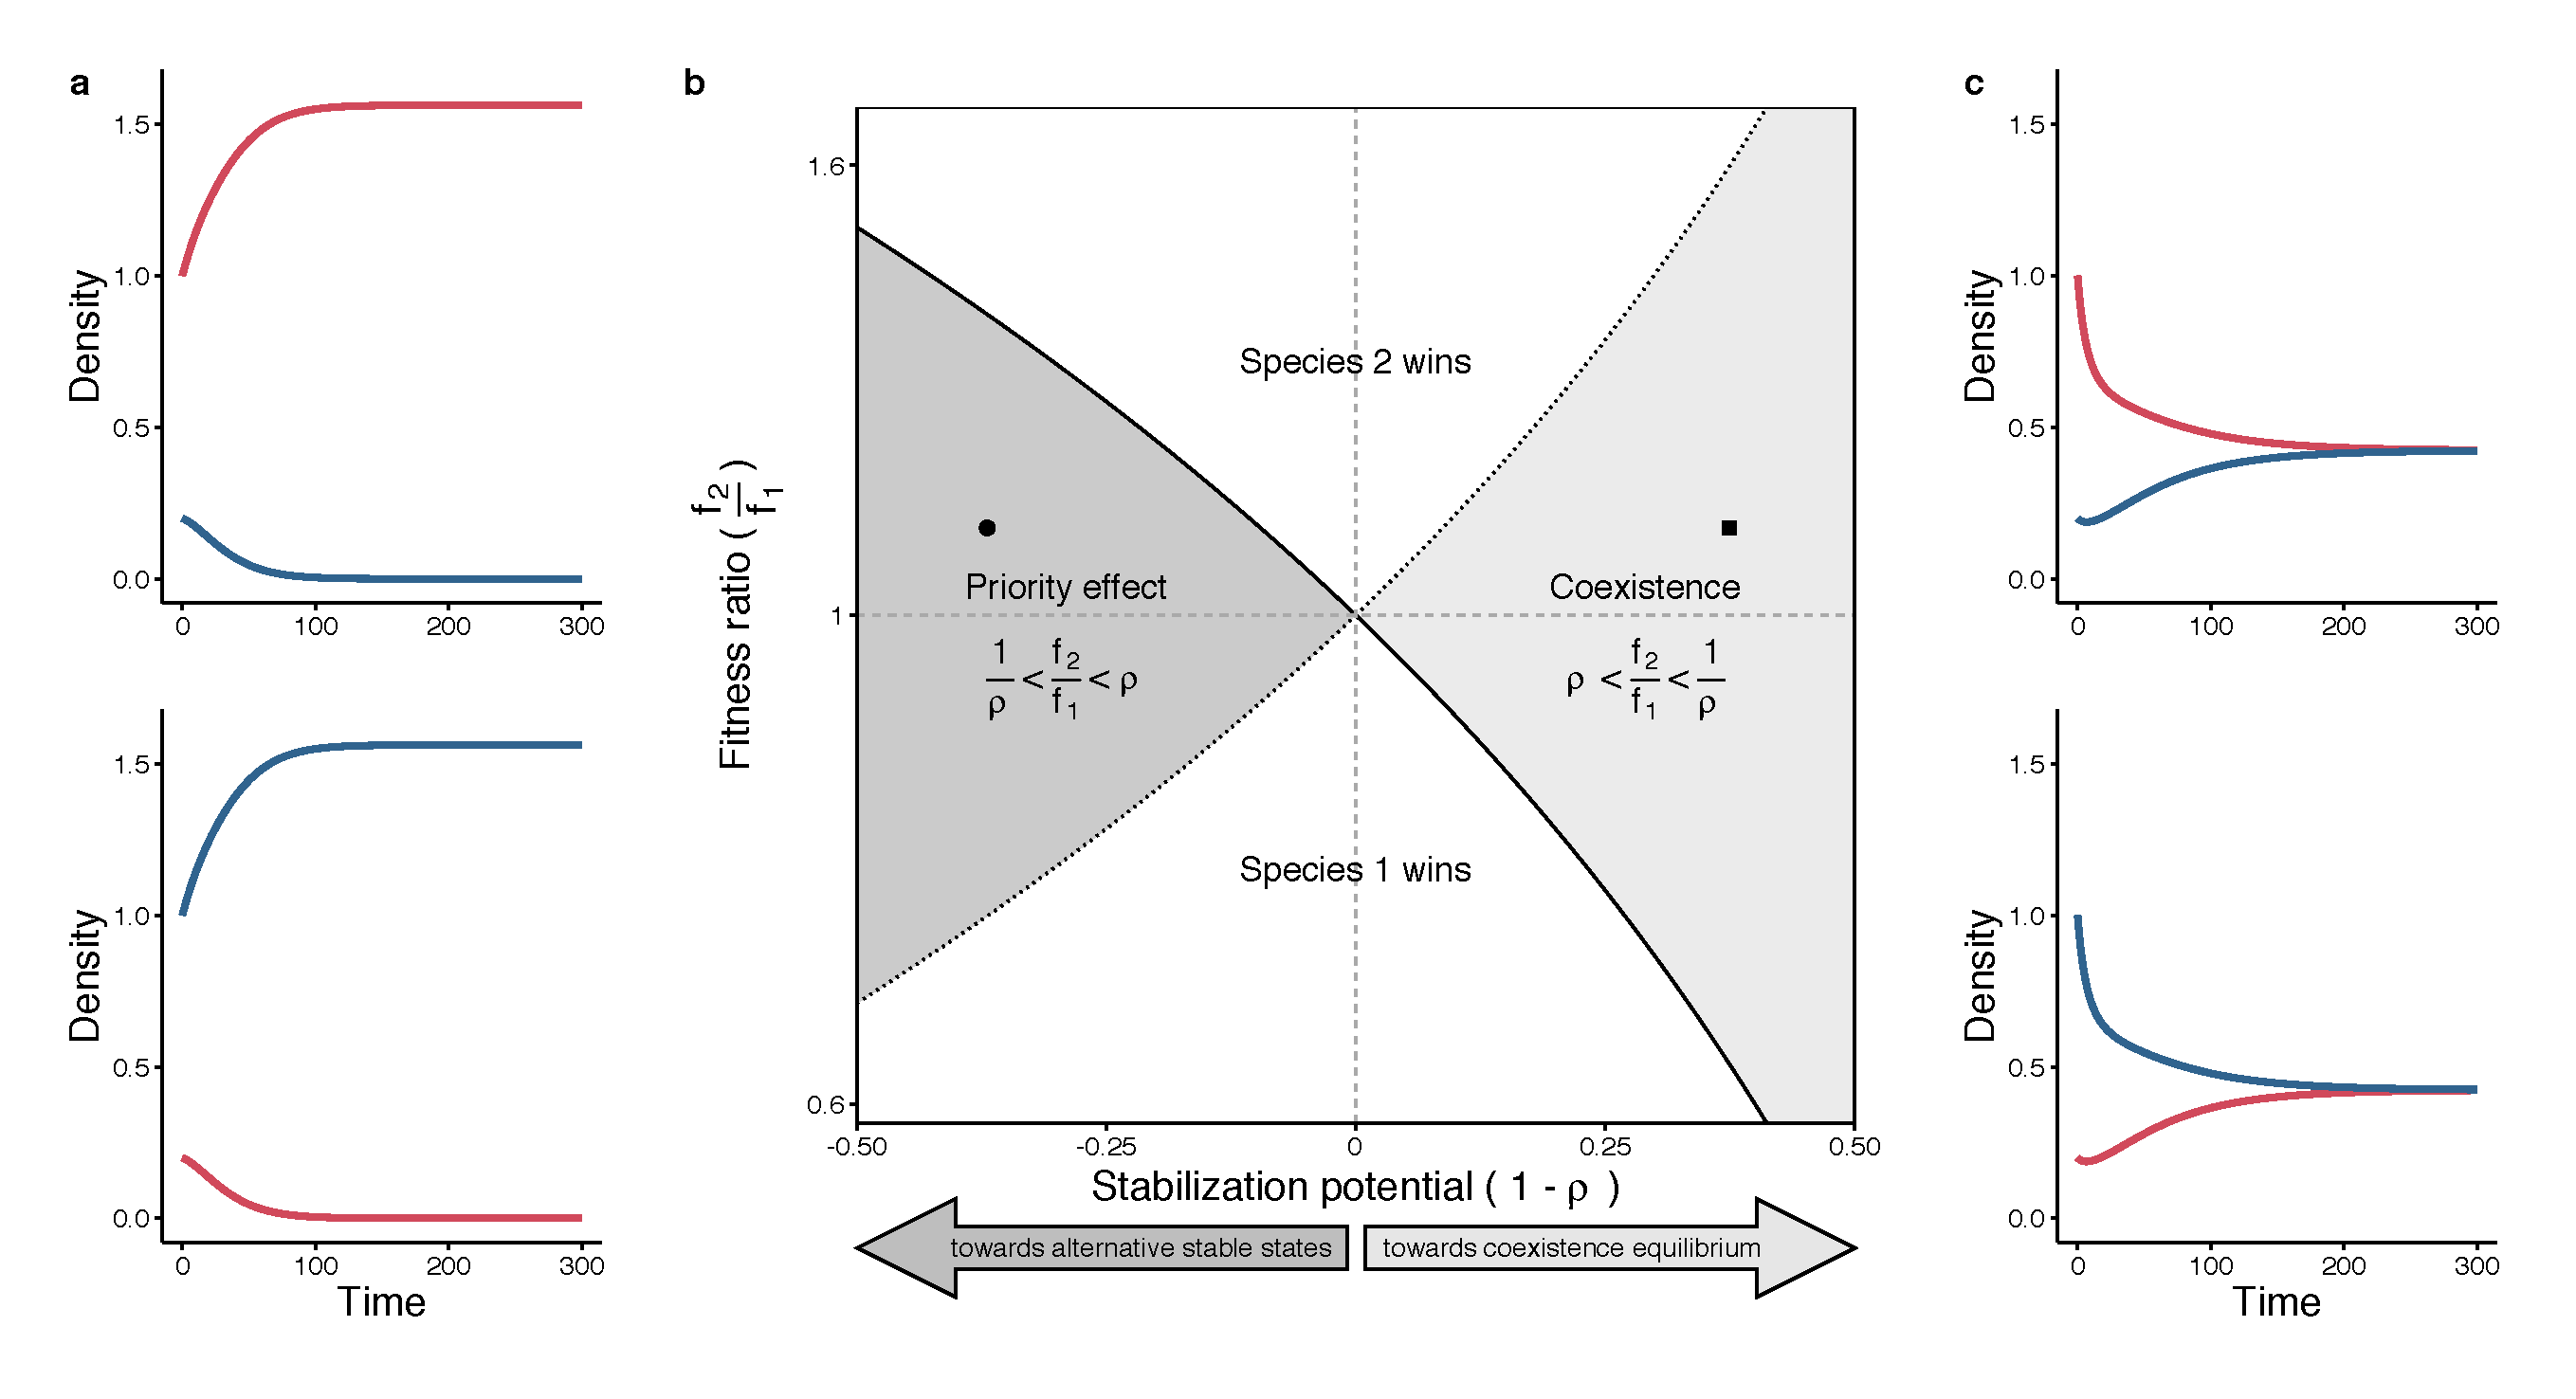
\includegraphics[width=14cm]{Chapter3/Conceptual.pdf}}
	\caption[Coexistence and priority effects in a Lotka--Volterra competition model.]
		{\hspace{1mm}Coexistence and priority effects in a Lotka--Volterra competition model. The community trajectories demonstrating priority effects (a) and stable coexistence (c) correspond to the position of the black circle and black square, respectively, in the central panel (b). In panel (b), the x-axis represents the stabilization potential (1 - $\rho$) and the y-axis represents the fitness ratio, $f_{2}/f_{1}$; the solid and dotted line represents the boundary where $f_{2}/f_{1}$ equals to $\rho$ and $1/\rho$, respectively. The upper and lower white area indicates the region where parameter combinations result in the dominance of species 2 (blue) and 1 (red), respectively; the right light gray and the left dark gray area indicates regions of stable coexistence and priority effects (parameter values and starting values provided in Appendix B).}
	\label{fig:FigBox}
\end{figure}



\newpage
\begin{figure}[h!]
	\centering
	\makebox[\textwidth][c]{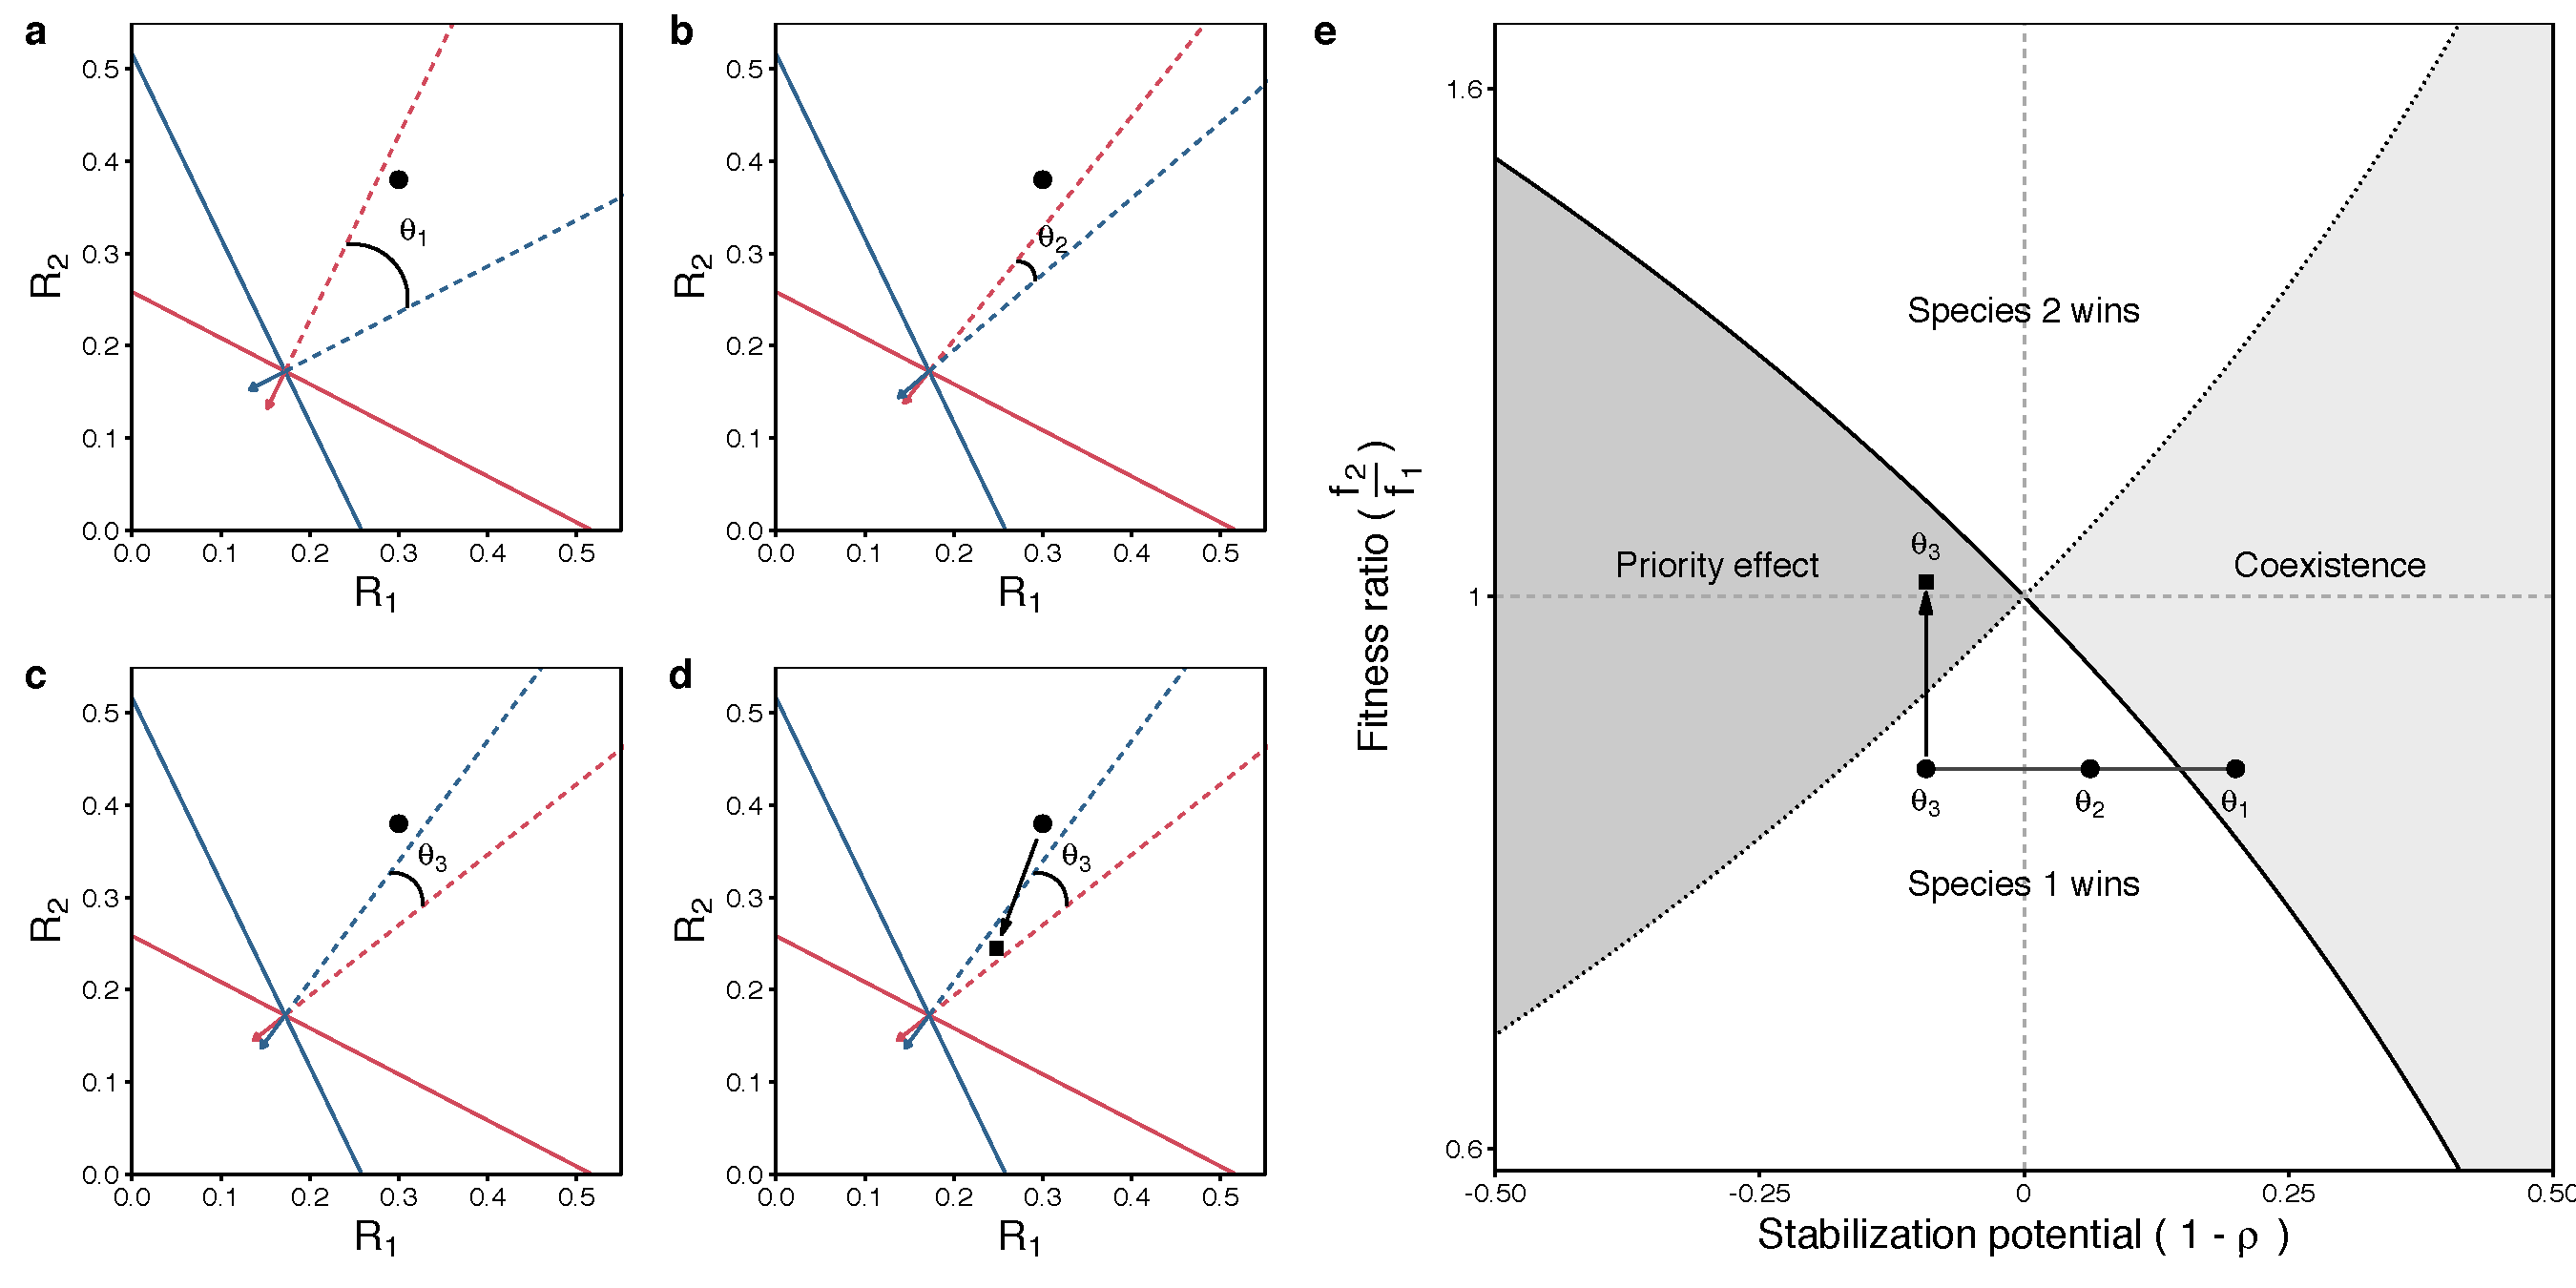
\includegraphics[width=14cm]{Chapter3/Fig1.pdf}}
	\caption[Effect of changing species' consumption vector and the supply ratio of two resources in a consumer-resource model on the fitness ratio and stabilization potential of coexistence theory.]
		{\hspace{1mm}Effect of changing species' consumption vector and the supply ratio of two resources in a consumer-resource model on the fitness ratio and stabilization potential (niche difference) of coexistence theory. In panel (a), the solid red and blue lines are the zero net growth isocline for each species (i.e., species 1 and 2, respectively); the solid lines with arrow heads are the respective consumption vectors; the dashed lines are the inverse of the vectors; and the black circle and square represent two different resource supply ratios (see footnote for technical definition of terms). In panel (a) -- (d), the red species benefits more from consuming $R_{2}$, while the blue species benefits most from $R_{1}$, as indicated by its lower $R^{*}$. In panel (e), the x-axis represents the stabilization potential (1 - $\rho$) and the y-axis represents the fitness ratio, $f_{2}/f_{1}$; and the right and left gray shaded area indicates the coexistence and priority effect region, respectively. The angles given by $\theta_{1-3}$ in panel (a) -- (d) correspond to the respective $\theta_{1-3}$ in panel (e). Note that the y-axis is on log-scale. Analytical treatment and simulation parameters provided in Appendix B.}
	\label{fig:Fig1}
\end{figure}



\newpage
\begin{figure}[h!]
	\centering
	\makebox[\textwidth][c]{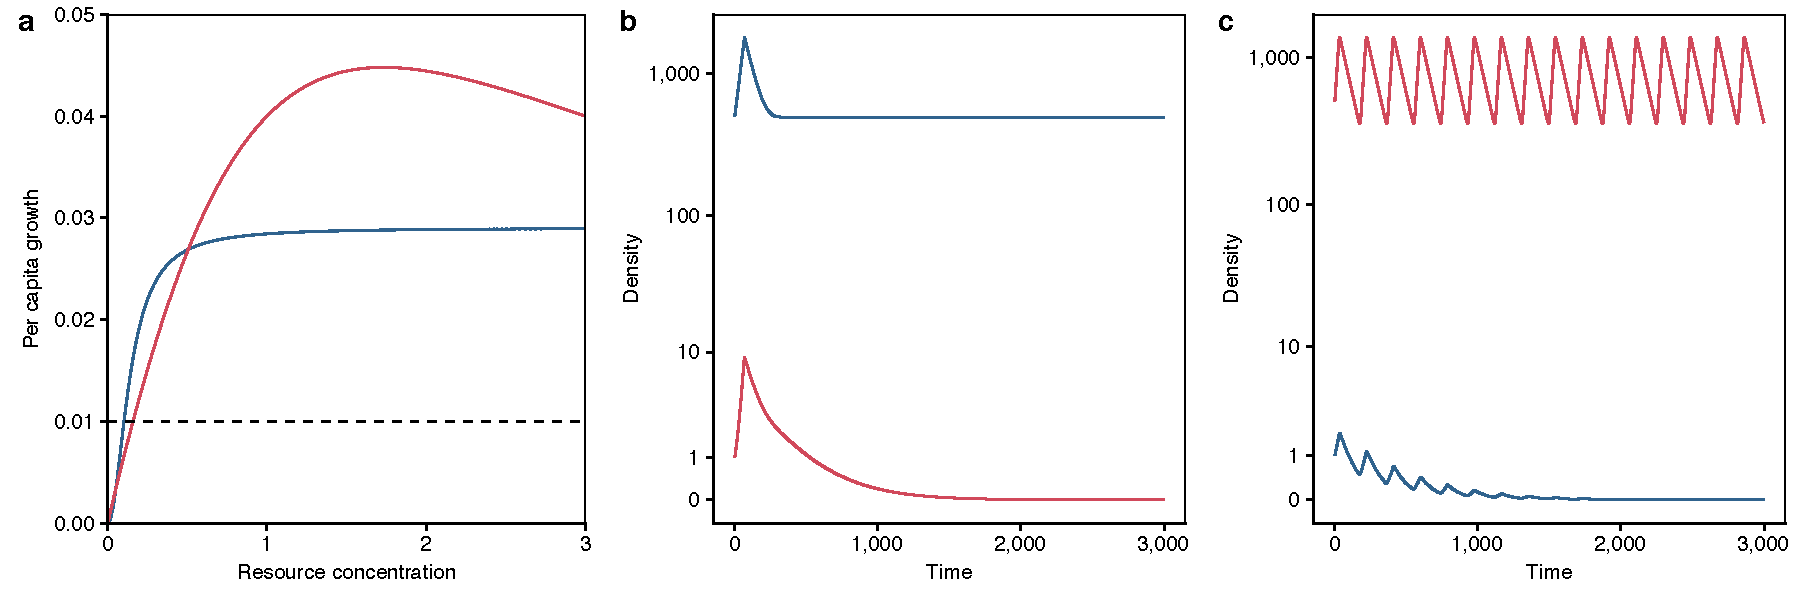
\includegraphics[width=14cm]{Chapter3/relnonlin.pdf}}
	\caption[Positive frequency dependence emergeing from endogenously generated resource fluctuations.]{\hspace{1mm}Positive frequency dependence emerges from endogenously generated resource fluctuations. In panel (a), blue is the better competitor at low resource levels and also suppresses fluctuations in the resource to its own advantage; Red is the better competitor at moderate resource levels, and, because of a highly nonlinear functional response owing to inhibited growth at high resource levels, generates fluctuations in the resource to its own advantage. Provided each species begins at a sufficiently higher density than its competitor, it is able to prevent its competitor from invading (b, c). Simulation parameters provided in Appendix B.}
	\label{fig:Fig2}
\end{figure}



\newpage
\begin{tcolorbox}[breakable, colback=white, leftright skip=-0.5cm]
	\label{fig:Box}
	\subsubsection*{Box 1 -- Coexistence and priority effects in a Lotka--Volterra competition model}
	Whether coexistence or priority effects emerges in a two-species Lotka--Volterra competition model depends on the relative magnitude of intra- and inter-specific competition. Consider the following Lotka--Volterra model:
	\begin{align*}
	\frac{dN_{1}}{dt}=r_{1}N_{1}\left ( 1-a_{11}N_{1}-a_{12}N_{2} \right ), \tag{3.5}\label{eq:LV1}
	\\~\\
	\frac{dN_{2}}{dt}=r_{2}N_{2}\left ( 1-a_{21}N_{1}-a_{22}N_{2} \right ). \tag{3.6}\label{eq:LV2}
	\end{align*}
	Each species intrinsic growth rate, $r_{1}$ and $r_{2}$, is negatively affected by intra-specific ($\alpha_{11}$ and $\alpha_{22}$) and inter-specific competition ($\alpha_{12}$ and $\alpha_{21}$). The two species stably coexist with positive densities if $\alpha_{11} > \alpha_{21}$ and $\alpha_{22} > \alpha_{12}$; that is, when intra-specific competition exceeds inter-specific competition. Under this scenario, each species exhibits negative frequency dependence since an increase in its abundance leads to larger negative impact on itself. Alternatively, when inter-specific effects exceed intra-specific effects, i.e., $\alpha_{11} < \alpha_{21}$ and $\alpha_{22} < \alpha_{12}$, each species exhibits positive frequency dependence; an increase in its abundance results in a larger negative impact on the competitor. This leads to priority effects in the form of alternative stable states. The community trajectory is attracted to one of the two monoculture equilibriums, dominated by either $N_{1}$ or $N_{2}$, depending on the initial abundance of the two species.
	\par
	
	
	The relationship between $\alpha_{ij}$'s and competition outcomes can be directly mapped onto the parameter space of the stabilization potential (1 - $\rho$, x-axis) and the fitness ratio ($f_{2}/f_{1}$, y-axis) (panel b of Fig.~\ref{fig:FigBox}, see main text). The solid ($f_{2}/f_{1} = \rho$) and dotted ($f_{2}/f_{1} = 1/\rho$) boundaries partition the parameter space into four distinct regions, each representing different outcomes of competition. The light gray area on the right ($\rho < \frac{f_{2}}{f_{1}} < 1/\rho$) indicates parameter combinations that result in stable coexistence. This requires $\rho$ to be bounded between zero and one, which is guaranteed when intra-specific competition is stronger than inter-specific competition. The dark gray area on the left ($1/\rho < \frac{f_{2}}{f_{1}} < \rho$) indicates the parameter space such that $\rho$ is greater than one, resulting in priority effects. 
\end{tcolorbox}

% \chapter{Effects of soil microbes on plant competition: a perspective from modern coexistence theory}
%\chaptermark{Positive frequency-dependence}
%\renewcommand{\sectionmark}[1]{}
\fancyhead[LE, RO]{\thepage}
\fancyhead[RE]{CHAPTER 4}
\fancyhead[LO]{SOIL MICROBES AND PLANT COEXISTENCE}
\fancyfoot{}
\renewcommand{\headrulewidth}{0pt}
\setlength{\parindent}{1cm}



\begin{comment}
\documentclass[hidelinks,letterpaper, 11pt]{article}
\usepackage{graphicx, bm, booktabs, lineno, array}
\usepackage[fleqn]{amsmath}
\usepackage{nicefrac}
\usepackage[compress,comma]{natbib}
\usepackage[right=1in, left=1in, top=1in, bottom=1in]{geometry}
\usepackage[parfill]{parskip}
\usepackage[usenames,dvipsnames]{color}
\usepackage[font=large,labelfont=bf,margin=1cm, labelsep = none]{caption} % caption formatting
\usepackage{setspace}
\usepackage{gensymb}
\usepackage{color}
\usepackage{sidecap}
%\usepackage{floatrow}
\usepackage{etoolbox}
\usepackage{tcolorbox}
\usepackage{newpxtext,newpxmath}
\tcbuselibrary{breakable}
%\usepackage{indentfirst}
\newbool{MyRefNumbers}
\usepackage{authblk}
\usepackage{hyperref}
\usepackage{mathpazo}
\usepackage[color=cyan, textsize=tiny]{todonotes}
\usepackage[font={normalsize}]{caption}
\usepackage{adjustbox}
\usepackage{array}
\usepackage{booktabs}
\usepackage{multirow}
\usepackage{tabularx}
% \usepackage{titling}

\setlength{\mathindent}{0pt}
\setlength{\parindent}{1cm}
% \makeatletter
% \makeatother
\pdfminorversion=3

% For table
\newenvironment{myindentpar}[1]%
{\begin{list}{}%
		{\setlength{\leftmargin}{#1}}%
		\item[]%
	}
	{\end{list}}
\newcommand*\samethanks[1][\value{footnote}]{\footnotemark[#1]}
\newcommand\blfootnote[1]{%
	\begingroup
	\renewcommand\thefootnote{}\footnote{#1}%
	\addtocounter{footnote}{-1}%
	\endgroup
}
\newcommand{+}{\raisebox{.4\height}{\scalebox{.6}{+}}}
\newcommand{\minus}{\raisebox{.4\height}{\scalebox{.8}{-}}}
% Command to recount supplement
\newcommand{\beginsupplement}{%
	\setcounter{table}{0}
	\renewcommand{\thetable}{S\arabic{table}}%
	\setcounter{figure}{0}
	\renewcommand{\thefigure}{S\arabic{figure}}%
}
% Command to center oversized images in floats
\newcommand{\centerfloat}{%
	\parindent \z@
	\leftskip \z@ \@plus 1fil \@minus \textwidth
	\rightskip\leftskip
	\parfillskip \z@skip}
\renewcommand\Affilfont{\fontsize{12}{12}\selectfont}
\newcommand{\ignore}[2]{\hspace{0in}#2}
\end{comment}



\begin{comment}
\begin{document}

\doublespacing
\title{Effects of soil microbes on plant competition: \\ a perspective from modern coexistence theory}
\author[* 1]{Po-Ju Ke}
\author[* 1, 2]{Joe Wan}
\affil[1]{Department of Biology, Stanford University, Stanford, California 94305-5020, USA}
\affil[2]{Institute of Integrative Biology, Department of Environmental Systems Science, ETH Z\"{u}rich, 8092 Z\"{u}rich, Switzerland}
\date{}
\maketitle
\blfootnote{* Both authors contributed equally}
\blfootnote{Correspondence author: Department of Biology, Stanford University, Stanford, California 94305-5020, USA. Phone: +1 650-721-1711. Email: pojuke@stanford.edu, jwan@student.ethz.ch}

\onehalfspacing
\noindent \textbf{Type of article:} Concepts and Synthesis\\
\noindent \textbf{Running head:} Soil microbes and plant coexistence\\
% \noindent \textbf{Keywords:} fitness difference, mutualism, niche difference, pathogens, plant--soil feedback\\
% \begin{myindentpar}{1cm}
	\textbf{Words in Abstract:} 233\\
	\textbf{Words in main text:} 7658\\
	% \textbf{Words in text boxes:} 241\\
	\textbf{Number of references:} 65\\
	\textbf{Number of figures:} 5\\
	\textbf{Number of tables:} 1\\
	\textbf{Number of text boxes:} 2\\
% \end{myindentpar}

% \noindent \textbf{Authorship statement:} PJK conceived the study; PJK and JW performed the analysis and wrote the manuscript.\\

% \noindent \textbf{Data accessibility statement:} No original data appear in this manuscript. Should the manuscript be accepted, all computer scripts supporting the results will be archived in an appropriate public repository such as Github, with the DOI included at the end of the article.\\

\doublespacing
\linenumbers
\end{comment}



\section{Abstract}
Growing evidence shows that soil microbes affect plant coexistence in a variety of systems. However, since these systems vary in the impacts microbes have on plants and in the ways plants compete with each other, it is challenging to integrate results into a general predictive theory.
To this end, we suggest that the concepts of niche and fitness difference from modern coexistence theory should be used to contextualize how soil microbes contribute to plant coexistence. Synthesizing a range of mechanisms under a general plant--soil microbe interaction model, we show that, depending on host-specificity, both pathogens and mutualists can affect the niche difference between competing plants.
However, we emphasize the need to also consider the effect of soil microbes on plant fitness differences, a role often overlooked when examining their role in plant coexistence.
Additionally, since our framework predicts that soil microbes modify the importance of plant--plant competition relative to other factors for determining the outcome of competition, we suggest that experimental work should simultaneously quantify microbial effects and plant competition. Thus, we propose experimental designs that efficiently measure both processes and show how our framework can be applied to identify the underlying drivers of coexistence. Using an empirical case study, we demonstrate that the processes driving coexistence can be counterintuitive, and that our general predictive framework provides a better way to identify the true processes through which soil microbes affect coexistence.
\medskip


\noindent \textbf{Keywords:} equalizing mechanisms, fitness difference, Janzen--Connell hypothesis, mutualism, niche difference, pathogens, plant--soil feedback, stabilizing mechanisms



\section{Introduction}
Ecologists have long invoked resource partitioning to explain the coexistence of competing species~\citep{Gause1934, tilman1982}, yet differences in resource use cannot fully account for plant diversity~\citep{Silvertown2004}. As a result, plant community ecologists have broadened their focus beyond plant--plant competition to address how interactions between trophic levels can affect plant coexistence \citep{Chesson2008, Mordecai2011, Lanuza2018, Cardinaux2018}. Growing evidence suggests that plants can influence the performance of both conspecifics and competitors by modifying soil microbial communities, an effect commonly studied under the framework of plant--soil feedbacks \citep{Bever1997, Bever2003}. Differences in the way competing plants interact with soil microbes might promote plant coexistence~\citep{Bever2003, Chung2016}. Alternatively, soil microbes could favor certain plants over their competitors, creating variation in species' relative abundance~\citep{Klironomos2002, Mangan2010} and invasion success~\citep{Reinhart2006, Ke2015}.
\par


% Problem: plant--soil interactions are complicated
The wide range of plant--soil microbe interactions makes it difficult to draw general conclusions about their effects on plant communities. In some systems, soil microbial communities may be predominantly harmful to plants due to high pathogen prevalence, while in other systems, beneficial microbes such as mycorrhizal fungi may play a more important role.
Moreover, the impacts of soil microbes depend on their degree of host-specificity. For example, pathogens can promote plant coexistence if they are host-specific \citep{Bell2006, Yamazaki2008, Bagchi2010} but may reduce plant diversity if a single species suffers greater attack \citep{Mordecai2011}. On the other hand, mycorrhizal fungi can hinder plant coexistence if the dominant species has greater mycorrhizal dependence \citep{Urcelay2003}, but may promote coexistence if they benefit not only their hosts but also their hosts' competitors \citep{Bever2002}.
Further adding to this complexity, plant--soil microbe interactions do not operate in isolation: their effect on coexistence must be considered within the context of plant--plant competition for limiting resources such as light and soil nutrients \citep{Callaway2004, Casper2007, Shannon2012, Crawford2017}. Indeed, variability in experimental results suggests that the relative importance of plant--soil microbe and plant--plant interactions may be highly system-specific \citep{Lekberg2018}. Because of the context-dependency of soil microbial interactions, an important question remains: what are the general conditions under which soil microbes promote plant coexistence?
\par


% Solution: modern coexistence framework
To synthesize the diverse roles that plant--soil microbe interactions play in plant communities, we draw on modern coexistence theory \citep{Chesson1990, Chesson2000, Chesson2008}. This framework uses two quantitative components to link species differences to competitive outcomes.
Niche differences summarize mechanisms that promote coexistence, such as differences in resource use~\citep{Chesson1990} or parasitism~\citep{Chesson2008}. These prevent competitive exclusion by giving each species an advantage when it is rare. On the other hand, fitness differences, such as differences in reproductive output or environmental tolerance, determine the ability of one species to exclude its competitor.
Thus, modern coexistence theory classifies processes mediating coexistence into two general categories: equalizing mechanisms, which decrease fitness differences between species, and stabilizing mechanisms, which increase niche differences between species~\citep{Chesson2000, Adler2007, Hillerislambers2012}.
Since coexistence requires the niche difference to be greater than the fitness difference between the two species, the two components form a common currency for understanding how mechanisms simultaneously affect coexistence.
Moreover, niche and fitness differences can be calculated for mathematical models \citep{Chesson2008} as well as experimental results \citep{Godoy2014, Gross2015, Kraft2015}, providing a quantitative link between empirical results and theoretical perspectives.
\par


% Summary of our goal
Taking advantage of the strengths of modern coexistence theory, we provide a unified framework that predicts and classifies the effects of soil microbes on plant coexistence.
We begin by presenting a theoretical framework for modeling interactions between plants and soil microbes (section ``\textit{Modeling plant--soil microbe interactions}''). In this section, we summarize previous theoretical treatments of plant--soil microbe interactions and outline a new mathematical model that links this field of research to the empirical and experimental tools of modern coexistence theory. In particular, we highlight the derivation of niche and fitness differences from the underling plant--soil microbe demographic model.
In the next section, we demonstrate how this model can be used to understand the outcome of plant--soil microbe interactions in diverse contexts (section ``\textit{Synthesizing microbial effects on plant coexistence}''). Here, we apply the model to four soil microbe-mediated scenarios drawn from the empirical literature and simulate their impacts on plant coexistence.
Synthesizing the results, we provide a general classification of soil microbial effects that clarifies: (1) when soil microbes stabilize plant coexistence, (2) when soil microbes equalize plant fitness, and (3) how soil microbes affect the importance of plant--plant competition.
Finally, we show how our framework can guide empirical studies (section ``\textit{Applying modern coexistence theory to plant--soil microbe interaction experiments}''). To do so, we propose experimental designs that efficiently quantify the full set of plant--plant and plant--soil microbe interactions. In a case study, we then apply our framework to existing experimental data and show how it uses the context of plant competition to identify the plant--soil microbe interactions most important for coexistence.
\par



\section{Modeling plant--soil microbe interactions}
% A quick overview of soil microbe-mediated plant-soil feedback models
\subsection{A brief overview of past modeling achievements}
We begin by summarizing previous theoretical work on plant--soil interactions to clarify the rationale behind our model.
In the first theoretical investigation of the role of soil microbes in plant coexistence, \citet{Bever1997} showed that plant-induced changes in the soil microbial community can promote coexistence if these changes negatively affect the growth rate of the plant relative to that of its competitors.
The model underlying this result focuses on plant and microbe frequencies (i.e., relative abundances): plant populations grow exponentially at rates determined by the frequencies of soil microbial communities, and coexistence conditions can be derived from the equations for plant frequencies. This approach allowed \citet{Bever1997} to define an ``interaction coefficient'', $I_{s}$, whose sign is mathematically a necessary (but not sufficient) criterion for plant coexistence \citep{Revilla2013, KeMiki2015}.
\citet{Bever1997} used this index to indicate the overall effects of soil microbes: when plants only interact with each other through their soil microbes, coexisting plants have a negative $I_{s}$ and is said to be experiencing ``negative plant--soil feedback''.
\par


The model of \citet{Bever1997} served as a starting point for subsequent theoretical studies (reviewed in \citealt{Bever2010, KeMiki2015}), including spatially-explicit treatments (e.g., \citealt{Eppinga2006}), frameworks explicitly representing soil nutrients (e.g., \citealt{Umbanhowar2005}), and multispecies models \citep{Kulmatiski2011, Eppinga2018}. Moreover, this theoretical treatment stimulated a productive line of empirical investigation \citep{Kulmatiski2008, vanderPutten2013}. Since the interaction coefficient in \citet{Bever1997} can be calculated by comparing plant performance in conspecific (home) and heterospecific (away) soils, it has allowed researchers to identify the direction of soil microbe-mediated feedbacks in a variety of systems (reviewed in \citealt{Bever2010, vanderPutten2013, Bever2015}).
\par


Subsequent work has addressed restrictions of the original approach.
Firstly, some follow-up work replaced the frequency-dependent microbial effects of the original model with density-dependent effects, which may be more appropriate for certain guilds of microbes (e.g., \citealt{Umbanhowar2005, Eppinga2006}).
Secondly, studies have incorporated more realistic plant population dynamics into the model. Originally, \citet{Bever1997} focused on the effects of soil microbes by assuming no self-limitation or competition in the plant populations. As a result, the original model cannot predict coexistence in systems where plants experience asymmetric competition. \citet{Bever2003} added Lotka--Volterra-type density-dependent plant competition to the original frequency-based plant--soil feedback model; \citet{Revilla2013} later analyzed this model and derived indexes corresponding to the original $I_{s}$ in \citet{Bever1997}. Nonetheless, these results have not provided a way to empirically predict the competitive outcome of combined plant--soil microbe and plant--plant interactions.
\par



\subsection{Model}
We build upon these previous models of reciprocal plant--soil microbe interactions to provide a theoretical model that (1) represents a more general set of plant--microbe and plant--plant interactions, (2) allows us to quantify niche and fitness differences, and (3) can be applied to predict competitive outcomes from greenhouse measurements of plant population dynamics.
In contrast to the approach in \citet{Bever2003}, which mixes frequency-dependent microbial effects with density-dependent plant--plant competition, we choose to consistently adopt density units. This approach has previously been used to model a variety of
% both pathogenic \citep{Eppinga2006} and mutualistic \citep{Umbanhowar2005}
soil microbes, and is compatible with experimental approaches which measure per-capita effects of competitors on plants.
\par


Our model adapts and generalizes the approach of \citet{Eppinga2006}, considering mutualistic soil microbes in addition to pathogens. The model tracks the densities of two competing plants and their associated soil microbes (summarized visually in Fig.~\ref{fig:Framework}a): $N_{A}$ and $N_{B}$ represent the density of competing plant species $A$ and $B$, respectively, while $S_{A}$ and $S_{B}$ represent the total density of each plant's root-associated soil microbial community. Each soil microbial community grows logistically with intrinsic growth rate $g_{A}$ and $g_{B}$ toward its carrying capacity $k_{A}$ and $k_{B}$:

\begin{equation}
\frac{dS_{A}}{dt} = g_{A}S_{A}\left ( 1-\frac{S_{A}}{k_{A}}\right )
\tag{4.1}\label{eq:SoilA}
\end{equation}
\begin{equation}
\frac{dS_{B}}{dt} = g_{B}S_{B}\left ( 1-\frac{S_{B}}{k_{B}}\right ) .
\tag{4.2}\label{eq:SoilB}
\end{equation}

\noindent Since the soil microbe community relies on resources that are supplied by plants (e.g., litter inputs, root exudates, or roots for direct colonization), we let the carrying capacity of the soil microbial community increase linearly with host plant density: $k_{i} = \phi_{i} \cdot N_{i}$, where $i = A$ or $B$. The parameter $\phi_{i}$ represents the ability of a plant individual to condition its soil microbes by supplying litter inputs or root exudates. As a result, when the host plant population increases, the carrying capacity of soil microbes also increases.
\par


Plant populations $N_{A}$ and $N_{B}$ grow at rates determined both by plant--plant competition and by the effects of soil microbes. As in the Lotka--Volterra competition model, the population growth of plants in the absence of competitors or microbes is given by the intrinsic growth rates $r_{A}$ and $r_{B}$. Plant--plant interaction is measured by $c_{ij}$, the linear effect of plant $j$ on plant $i$. We build on this classic model by incorporating direct interaction between plants and soil microbial communities: $\sigma_{ij}$, the soil microbe interaction coefficient, gives the linear effect of the microbial community specific to plant $j$ on plant $i$ (see \citealp{Eppinga2006} and \citealp{Aguilera2011} for nonlinear functional response). Note that unlike in the model of \citet{Bever2003}, here $c_{ij}$ and $\sigma_{ij}$ have the same density-based units. Accordingly, plant population dynamics are described as follows:

\begin{equation}
%\frac{dN_{A}}{dt } = r_{A}N_{A} \left( 1 + \frac{c_{AA}N_{A}+c_{AB}N_{B}}{K_{A}} \right) + \left( \sigma_{AA}S_{A}+\sigma_{AB}S_{B} \right)N_{A},
\frac{dN_{A}}{dt} = r_{A}N_{A} \left( 1 + c_{AA}N_{A}+c_{AB}N_{B} + \sigma_{AA}S_{A}+\sigma_{AB}S_{B} \right)
\tag{4.3}\label{eq:Na}
\end{equation}
\begin{equation}
%\frac{dN_{B}}{dt } = r_{B}N_{B} \left( 1 + \frac{c_{BB}N_{B}+c_{BA}N_{A}}{K_{B}} \right) + \left( \sigma_{BA}S_{A}+\sigma_{BB}S_{B} \right)N_{B}.
\frac{dN_{B}}{dt} = r_{B}N_{B} \left( 1 + c_{BA}N_{A}+c_{BB}N_{B} + \sigma_{BA}S_{A}+\sigma_{BB}S_{B} \right) .
\tag{4.4}\label{eq:Nb}
\end{equation}

\noindent For our purpose, we assume that plant--plant interactions are competitive ($c_{ij} < 0$, thus hereafter referred as plant--plant competition), where a more negative $c_{ij}$ represents stronger competition.
On the other hand, each species-specific soil microbial community may be either detrimental ($\sigma_{ij} < 0$) or beneficial ($\sigma_{ij} > 0$) to each plant.
A more negative $\sigma_{ij}$ represents a stronger detrimental effect of a soil microbial community on a plant, whereas a more positive $\sigma_{ij}$ represents a greater beneficial effect.
Since $\sigma_{ij}$ represents the entire effect of a microbial community, it may summarize a variety of microbial guilds. Thus, on the whole, each specific microbial community may be considered to have a net pathogenic ($\sigma_{ij} < 0$) or mutualistic effect ($\sigma_{ij} > 0$) relative to the case where no plant-specific soil conditioning occurs.
Additionally, we note that our model is able to represent shared soil microbial associates through their net effect on $\sigma_{ij}$ (see Appendix C.1, where we derive Eqns.~\ref{eq:Na} -- \ref{eq:Nb} from a model that explicitly represents microbial species).
\par



\subsection{Quantifying the components of modern coexistence theory}
% Model analysis overview -- separating ND and FD from the PSF model
Modern coexistence theory provides a specific formula to quantify the stabilizing and equalizing components of coexistence for species whose dynamics can be approximated by a Lotka--Volterra model \citep{Chesson1990, Chesson2008b, Chesson2013ecosys}. To take advantage of the theory, we applied separation of timescales to transform our model into the standard Lotka--Volterra form. In particular, we assumed that the dynamics of soil microbes were sufficiently fast compared to that of the plants (see Box 1 and Appendix C.2 for detailed derivation and interpretation). While we focused on our general theoretical framework, we note that timescale separation can be applied to derive niche overlap and fitness ratio for a variety of models of plant--soil microbe interactions (Appendix C.1).
\par


A key feature in our mathematical derivation is the phenomenological interaction coefficient, $\alpha_{ij}$ (i.e., the competition coefficient of the Lotka--Volterra appoximation, Eqn.~\ref{eq:alpha} in Box 1). This coefficient represents the total per-capita effect of species on conspecific or heterospecific plants, summarizing the combined effect of plant--plant competition ($c_{ij}$) and that of soil microbes ($\sigma_{ij}$). As $\alpha_{ij}$ corresponds to the interaction coefficients measured by plant competition experiments, this result links our framework to existing experimental methods for quantifying the modern coexistence theory components.
After transforming the model, we used the formulas from \citep{Chesson2008} to quantify niche overlap and fitness ratio between the two species. Doing so, we were able to examine how plant--plant competition and soil microbial effects interactively determine coexistence.
\par



\section{Synthesizing microbial effects on plant coexistence}
In this section, we demonstrate how our model can be applied to predict the effect of soil microbes, and show that the two components of modern coexistence theory are capable of synthesizing a diverse set of microbial processes that affect plant coexistence. We begin by applying the formulas for niche overlap and fitness ratio (Box 1) to study four different plant--soil microbe interaction scenarios, each representing a well-documented empirical example of how soil microbes can influence plant performance. In each case, we determined whether soil microbes promoted or prevented coexistence, and whether this effect was mediated by niche, fitness, or both components. Generalizing these results, we then present a small set of categories that can predict how a large number of soil microbe-mediated processes affect plant coexistence.
\par



\subsection{Simulating different plant--soil microbe interaction scenarios}
% Model analysis overview -- simulation scenarios
As shown in Figure~\ref{fig:Framework}b, we considered the following scenarios: (1) a Janzen--Connell scenario, where both plants experience increasingly negative conspecific microbial effects driven by host-specific pathogens \citep{Janzen1970, Connell1971}; (2) an enemy release scenario, where negative microbial effects on one plant are alleviated \citep{Keane2002, Reinhart2006}; (3) a mutual facilitation scenario, where the beneficial mycorrhizal fungus hosted by each plant has a increasingly positive effect on the competitor of its host \citep{Bever2002}; and (4) a differential soil conditioning scenario, where one plant allocates more photosynthetic products to support a greater population of beneficial microbes \citep{Zheng2015, Norby1987}. Figure~\ref{fig:Framework}b summarizes these scenarios using thick arrows to highlight each set of characteristic parameters. Together, the four scenarios encompass a wide array of microbial functional groups, ranging from pathogenic to beneficial and from specialists to generalists. See also Table~\ref{table:psf_recipe} for a list of other scenarios that can be considered using our modeling framework.
\par


% Simulation results
For each of the four scenarios, we ran simulations to quantify how varying soil microbial effects (i.e., the magnitude of $\sigma_{ij}$ or $\phi_{i}$; see Fig.~\ref{fig:Scenario_Battleaxes} and Table~\ref{table:Parameters} for parameter values) affected overall competition.
We visualized these results on the parameter space of niche difference and fitness ratio (Box 2). Although this variation always affected both of these components (arrows of Fig.~\ref{fig:Scenario_Battleaxes}), the effect of some scenarios was primarily mediated by a single mechanism.
The Janzen--Connell (Fig.~\ref{fig:Scenario_Battleaxes}a) and mutual facilitation (Fig.~\ref{fig:Scenario_Battleaxes}c) scenarios always increased niche differences, but their effects on fitness ratio were smaller and inconsistent. Thus, in these scenarios, soil microbes acted predominantly as a stabilizing mechanism. On the other hand, enemy release (Fig.~\ref{fig:Scenario_Battleaxes}b) primarily affected the fitness ratio; thus, soil microbes in this scenario primarily had an equalizing effect and promotes coexistence when they benefited the inferior competitor. Finally, both mechanisms were important in the soil conditioning case (Fig.~\ref{fig:Scenario_Battleaxes}b).
\par


To understand the interaction between plant--soil microbe interactions and plant--plant competition, we simulated each of the four scenarios with different strengths of plant--plant competition $c_{ij}$, producing the different-colored arrows in Figure~\ref{fig:Scenario_Battleaxes}.
We varied one of the four $c_{ij}$ at a time while keeping the other three fixed (see Fig.~\ref{fig:Scenario_Battleaxes} and Table~\ref{table:Parameters} for parameter values).
The range of niche differences and fitness ratio generated by different values of $c_{ij}$ indicates importance of plant--plant competition in determining competitive outcome. We showed that the effect of the illustrated coefficients could be either reduced (Fig.~\ref{fig:Scenario_Battleaxes}a) or amplified (Fig.~\ref{fig:Scenario_Battleaxes}b--d) by soil microbial effects, suggesting the need to consider interactions between plant--plant and plant--soil microbe interactions.
However, for other coefficients, plant--soil microbe interactions did not alter the qualitative importance of plant--plant competition (Appendix C.4: Fig.~\ref{fig:Janzen_Connell_everything}-\ref{fig:Soil_Conditioning_everything})
In general, these interactive effects only occurred for the forms of plant--plant competition ($c_{ij}$) corresponding to the soil microbial effects ($\sigma_{ij}$) that were varied by the plant--soil microbe interaction scenario.
Below, we detail the simulation results for each of our four scenarios.
\par



\subsubsection*{Janzen-Connell scenario}
According to the Janzen--Connell hypothesis, a classic mechanism of natural enemy-mediated coexistence, species build up high densities of host-specific natural enemies near parent trees \citep{Augspurger1984}. We focused on a version of this mechanism mediated by soil pathogens, corresponding to the negative plant--soil feedbacks measured in both temperate~\cite{Bennett2017} and tropical~\citep{Mangan2010} forest systems. In the simulation, plants cultivated soil pathogen communities which are only slightly harmful to the non-cultivating species ($\sigma_{AB} = -0.4$, $\sigma_{BA} = -0.5$). Beginning with $\sigma_{AA} = \sigma_{BB} = -0.032$ (slightly weaker than interspecific effects), we strengthened the impact of both soil pathogen communities on their cultivating plants until both parameters reached $-6.0$ (much stronger than interspecific effects).
\par


This promoted coexistence primarily by increasing niche difference between the competing plant species: in other words, soil microbes acted primarily as a stabilizing mechanism. Nonetheless, varying Janzen--Connell strength also affected fitness ratio, which was sometimes enough to change the identity of the dominant competitor (Fig.~\ref{fig:Scenario_Battleaxes}a, $c_{AA} = -1$), but this effect was small relative to the change in niche difference and varied depending on plant--plant competition. As the negative effect of host-specific pathogens increased, intraspecific plant--plant competition ($c_{AA}$ and $c_{BB}$) became less important in determining overall competitive outcome. This can be seen in Fig.~\ref{fig:Scenario_Battleaxes}a, where the changes in fitness ratio and niche difference caused by changing $c_{AA}$ decreased with intensifying soil microbial effects. However, we did not observe a similar effect for interspecific competition ($c_{AB}$ and $c_{BA}$), which remained qualitatively important for determining fitness ratio regardless of Janzen--Connell strength (Appendix C.4: Fig.~\ref{fig:Janzen_Connell_everything}).
\par



\subsubsection*{Enemy release scenario}
Enemy release occurs when species experience decreased pressure from natural enemies in their introduced range. While release from species-specific natural enemies has received greater attention, the effect also encompasses decreased pressure from generalist natural enemies~\citep{Keane2002}; here, we considered both kinds of natural enemies. Inspired by evidence plants are less negatively affected by soil pathogens in their introduced ranges \citep{Reinhart2006}, we considered an introduced species (plant $B$) competing with a native species (plant $A$). Beginning with a scenario where soil pathogen communities affect both plants ($\sigma_{AA} = \sigma_{AB} = -0.5;\ \sigma_{BA} = \sigma_{BB} = -2.0$), we alleviated the effect of both pathogen communities on B by increasing $\sigma_{BA}, \sigma_{BB}$ until $\sigma_{BA} = \sigma_{BB} = 0$ (representing complete enemy release).
\par


The enemy release scenario had a strong effect on fitness ratios: as plant $B$ became increasing released from enemy effects, its fitness increased relative to that of its competitor. In the case examined here, this allowed the two plants to coexist. More generally, such an effect should be expected to promote coexistence if it benefits the inferior competitor to an intermediate degree (Appendix C.4: Fig.~\ref{fig:Enemy_Release_everything}). Enemy release had a smaller effect on niche difference, and the direction of this effect varied according to $c_{BA}$ (different arrows in Fig.~\ref{fig:Scenario_Battleaxes}b). As the impact of natural enemies on plant $B$ decreased, its sensitivity to plant--plant competition ($c_{BA}$ and $c_{BB}$) became increasingly important for determining fitness ratio and niche difference (shown for $c_{BA}$ in Fig.~\ref{fig:Scenario_Battleaxes}b). In contrast, the remaining coefficients ($c_{AB}$ and $c_{AA}$, representing the sensitivity of plant $A$ to plant--plant competition) did not produce this interactive effect (Appendix C.4: Fig.~\ref{fig:Enemy_Release_everything}).
\par



\subsubsection*{Mutual facilitation scenario}
While much work on microbe-mediated plant coexistence has focused on pathogens, \citet{Bever2002} proposed that conditioning of mutualist communities can promote plant coexistence if this condition favor plants' competitors (i.e., causes plants to facilitate one another). Beginning with a scenario where the soil mutualist communities benefit their cultivating hosts ($\sigma_{AA} = \sigma_{BB} = 0.5$) but not their hosts' competitors ($\sigma_{AB} = \sigma_{BA} = 0.0$), we increased the degree of mutual facilitation $\sigma_{AB}, \sigma_{BA}$ until each soil community was much more beneficial to its hosts' competitor than to its own host ($\sigma_{AB} = \sigma_{BA} = 2.0$).
\par


As in the Janzen--Connell scenario, the mutual facilitation scenario always increased niche difference between the two competitors; in some cases, this was enough to result in coexistence. Additionally, mutual facilitation affected fitness ratio, but the direction of changes was inconsistent (different arrows in Fig.~\ref{fig:Scenario_Battleaxes}c).
Increasing mutual facilitation amplified the effect of interspecific plant--plant competition ($c_{AB}$ and $c_{BA}$), but not that of intraspecific competition ($c_{AA}$ and $c_{BB}$), on fitness ratio and niche difference (shown for $c_{AB}$ in Fig.~\ref{fig:Scenario_Battleaxes}c, see also Appendix C.4: Fig.~\ref{fig:Mutual_Facilitation_everything}). Thus, though the Janzen--Connell and mutual facilitation scenarios both increased niche difference, they interacted differently with plant--plant competition.
\par



\subsubsection*{Differential soil conditioning}
Differences in the strength of soil microbial effects on plants may also be mediated by differences in plants' ability to cultivate soil microbial communities. For instance, the amount of fixed carbon provided by plants to their mycorrhizal mutualists may vary depending on the environmental context \citep{Zheng2015, Norby1987} and on plant competitive strategy \citep{Hoeksema2010}. We considered a pair of competing plants, each cultivating a mutualist community ($\sigma_{AA} = 0.5;\ \sigma_{AB} = 0.25;\ \sigma_{BB} = 0.20;\ \sigma_{BA} = 0.10$). We began with the scenario where both plants had equal conditioning ability, represented by the microbial carrying capacity $\phi_{A} = \phi_{B} = 0.025$. We then increased the ability of plant $B$ to condition its soil community by increasing $\phi_{B}$ up to $2.5$.
\par


Depending on plant--plant competition parameters, increased soil conditioning by plant $B$ could either promote or prevent coexistence, an effect mediated by both fitness and niche components (Fig.~\ref{fig:Scenario_Battleaxes}d). Mathematically, this context-dependent result occurs because changing the conditioning ability of $B$ affects the invasion growth rate of plant $A$, but not that of plant $B$ (Appendix C.3). Examining the interaction of plant--plant competition parameters with soil conditioning, we found that soil conditioning increased the importance of plant $B$'s competitive effect ($c_{AB}$ and $c_{BB}$; shown for $c_{AB}$ in Fig.~\ref{fig:Scenario_Battleaxes}d) but did not change the qualitative importance of the competitive effect of plant $A$ ($c_{BA}$ and $c_{AA}$; Appendix C.4: Fig.~\ref{fig:Soil_Conditioning_everything}).
\par



\subsection{A general categorization of soil microbial effects}
The above simulations illustrate that interactions between plants and soil microbes can have diverse effects on coexistence. Some mechanisms primarily affected niche differences, others affected fitness, and still others acted through a combination of the two components; moreover, each mechanism interacted differently with plant--plant competition.
Given these diverse results, how can we synthesize existing perspectives into a unified understanding of how soil microbes influence plant coexistence?
\par


Our study provides a general framework for integrating a diverse set of plant--soil microbe interactions with plant--plant competition. In Table \ref{table:psf_recipe}, we show how the effects of a microbe-mediated process on niche and fitness differences, as well as its impact on the relative importance of plant--plant competition, can be predicted via understanding which interactions are being modified.
We identify four ways a process can affect the plant--microbe interaction network, representing each possible pair of plant--soil microbe interactions $\sigma_{ij}$ (column I). Within each of the types of network effects, we contrast processes that increase the overall negative interaction among plants (i.e., increase $\alpha_{ij}$, the total per-capita effect of one plant on another) with those that decrease the overall negative interaction (column II). In other words, we consider whether the indirect effect of microbe intensifies or mitigates plant competition. Importantly, these changes are not specific to pathogens or mutualists: for instance,  an increase in a plants' overall negative impact can result from strengthening the effect of pathogens or from weakening the effects of mutualists.
\par


Based on this general categorization, the effect of a process on the underlying interaction network determines whether it primarily affects niche or fitness (column III) and predicts which forms of plant--plant competition ($c_{ij}$) will change in its importance for coexistence (column IV). In both cases, the direction of these changes depends on whether a process increases or decreases the overall negative interaction among plants. Thus, our framework can be applied to predict the effects of various soil microbe-mediated processes considered in the empirical literature (column V), including the four focal scenarios simulated in this study (shown in bold type).
\par



\subsubsection*{Soil microbes and stabilizing niche differences}
Our findings confirm that soil microbes can promote plant coexistence by favoring each plant when it is rare an effect frequently discussed in the literature \citep{Bever1997, Hart2003, Bever2003, KeMiki2015}.
This effect, often termed negative plant--soil feedback \citep{Bever1997}, corresponds to the niche difference component of modern coexistence theory.
Our approach shows that this occurs when a microbe-mediated process causes the negative impact of a plant on conspecifics to increase (type a in Table \ref{table:psf_recipe}; e.g., Janzen--Connell scenario, Fig.~\ref{fig:Scenario_Battleaxes}a) or that on its competitors to decrease (type b in Table \ref{table:psf_recipe}; e.g., mutual facilitation scenario, Fig.~\ref{fig:Scenario_Battleaxes}b).
This result is in accordance with those from \citeauthor{Bever1997}'s \citeyearpar{Bever1997} exponential model, which showed that both pathogens and mutualists may promote plant coexistence.
% Our predictions are in accordance with those from the original model of \citet{Bever1997}, despite the model's different (exponential) formulation. In particular, Bever's model showed that both pathogens and mutualists may create negative feedbacks ($I_{s} < 0$), in some cases allowing coexistence.
Our application of modern coexistence theory adds to this classic perspective by linking it to the broader empirical literature on plant coexistence and providing a more thorough exploration of the contexts under which soil microbes affect coexistence.
\par


This perspective synthesizes a diverse range of stabilizing and destabilizing soil microbial processes from the literature.
% Depending on host specificity, both pathogens and mutualists may stabilize or destabilize plant coexistence.
We confirm that species-specific soil pathogens indeed promote coexistence by increasing niche differences, thus acting as a stabilizing mechanism~\citep{Petermann2008}. We also note that stabilization is not unique to soil pathogens: mutualists can stabilize coexistence if they also confer their mutualistic benefits to their host plant's competitors~\citep{Bever1999, Bever2002}.
In contrast to the case of mutual facilitation, we also predict that host-specific soil mutualists can lead to priority effects by increasing niche overlap, thus acting as a destabilizing mechanism (\textit{sensu} \citealt{Fukami2016}). Empirical evidence of such positive feedbacks comes from systems where arbuscular mycorrhizal plants compete with ectomycorrhizal plants~\citep{McGuire2007, Bennett2017, Kadowaki2017}.
Accordingly, we suggest that experimental approaches informed by modern coexistence theory \citep{Hart2018} may further elucidate links between mycorrhizal strategy and plant community dynamics.
\par


Despite similar stabilizing effects, different soil microbial processes may have different effects on the importance of plant--plant competition, an aspect not captured by the original \citet{Bever1997} model and its related $I_{s}$ index.
For example, while host-specific pathogens contribute to stabilization and can overwhelm the effect of intraspecific plant--plant competition (Fig. \ref{fig:Scenario_Battleaxes}a), interspecific competition remains important in determining the degree of stabilization required for coexistence (Appendix C.4: Fig.~\ref{fig:Janzen_Connell_everything}). This prediction emphasizes the importance of considering interspecific competition when studying conspecific negative density dependence \citep{LaManna2017}.
In other cases (e.g., mutual facilitation) microbe-mediated processes may amplify the role of certain forms of plant--plant competition (here, interspecific competition). This is in line with empirical findings that mycorrhizal fungi can intensify plant competition for light \citep{Facelli1999} by modifying the shoot-to-root ratio of plants \citep{Veresoglou2012}.
% Importantly, these results would not be observed if studies only focused on plant--soil microbe interactions since microbes generated similar stabilizing effect in both cases.
Such differences between scenarios, despite their similar stabilizing effect, highlight the importance of considering soil microbial effects within the context of plant--plant competition \citep{Callaway2004, Casper2007, Shannon2012, Crawford2017, Peay2018}.
% While the importance of plant--plant competition was incorporated in later versions of the Bever model \citep{Bever2003, Revilla2013}, most of their analyses either assumed equal competitive ability among plants or only focused on the overall strength of plant--plant competition.
Here, we suggest that further categorizing plant--soil microbe interactions with our framework provides concrete predictions of how the two processes interact (Table~\ref{table:psf_recipe}).
\par



% Neglected role of fitness effects
\subsubsection*{The need to consider soil microbial effects on fitness}
In addition to their frequently-cited stabilizing role, soil microbes may also affect the fitness of competing plants \citep{Mordecai2011}.
However, this aspect of soil microbial effects is often overlooked in frequency-based models (e.g., \citealt{Bever1997}, but see \citealt{Eppinga2018}).
Supporting the notion that niche and fitness differences are not independent \citep{Letten2017, Barabas2018}, we found that soil microbes always affected fitness (Fig.~\ref{fig:Scenario_Battleaxes}). Mathematically, this occurs because changing any soil microbial coefficient always affects both $\rho$ and $\frac{f_{2}}{f_{1}}$ (Box 1).
Furthermore, fitness is sometimes key to predicting coexistence: when a process alters the sensitivity of one plant to both microbial communities, its effect on coexistence is primarily mediated by equalizing mechanisms (type c in Table \ref{table:psf_recipe}; e.g., enemy release scenario, Fig.~\ref{fig:Scenario_Battleaxes}c). In these cases, soil microbes promote coexistence if they benefit the plant with lower fitness.
Observed tradeoffs between plant--plant competition and responsiveness to mutualists~\citep{Grman2012} or defense against soil pathogens~\citep{Rasmann2011} may thus promote coexistence by acting as equalizing mechanisms. Again, we suggest that simultaneous measurement of microbial effects and plant--plant competition is necessary to assess the importance of these tradeoffs.
\par


As in other cases, these microbe-mediated processes may affect the importance of plant--plant competition for plant fitness. For instance, fitness differences generated by intraspecific plant competition were erased by host-specific pathogens in the Janzen--Connell scenario (Fig.~\ref{fig:Scenario_Battleaxes}a), but were not affected in the mutual facilitation scenario (Appendix C.4: Fig.~\ref{fig:Mutual_Facilitation_everything}).
Another example comes from the enemy release scenario: we predict that as an invader (here, plant $B$) becomes increasingly released from enemies, its sensitivity to competition ($c_{BA}$ and $c_{BB}$) will become increasingly important for determining competitive outcome (Appendix C.4: Fig.~\ref{fig:Enemy_Release_everything}).
This prediction has practical implications: when considering the invasive potential of an enemy-released exotic plant, for instance, it may be particularly important to evaluate its sensitivity to plant--plant competition. That is, in the presence of enemy release, the most successful invaders should be those with the highest tolerance of competition from natives (least negative $c_{BA}$), rather than those with the strongest negative impact on natives (most negative $c_{AB}$).
In summary, the different effects of soil microbes on plant fitness, a crucial determinant of coexistence highlighted in modern coexistence theory, emphasizes the importance of the competitive context in which plant--soil microbe interactions occur.
\par


% Microbial effects on both plants merits increased consideration
Though some processes are primarily equalizing or stabilizing, we also identify a set of processes where both effects must be considered (type d in Table \ref{table:psf_recipe}). Namely, when a mechanism varies a single soil community's effect on both plants (e.g., differential soil conditioning scenario, Fig.~\ref{fig:Scenario_Battleaxes}d), its effect on coexistence is mediated by both niche difference and fitness ratio. This occurs because a soil microbial community can only affect the invasion growth of the non-cultivating plant. Thus, it affects both niche difference and fitness ratio, and the direction of these effects varies depending on plant--plant competition.
\par


Many biologically relevant processes belong to this category. For instance, pathogens vary in their virulence~\citep{Reinhart2010} and plants' ability to condition mutualists may vary due to environmental conditions~\citep{Zheng2015, Norby1987}. Under these cases, it is not possible to draw a general conclusion on the effect of soil microbes on plant coexistence because the direction of these effects are context-dependent. To further decipher the role of soil microbes for these processes here, we emphasize the need for empirical work to directly measure the strength of both plant--plant and plant--soil microbe interactions.
\par



\section{Applying modern coexistence theory to plant--soil microbe interaction experiments}
Our framework demonstrates the importance of the interaction between soil microbial effects and plant--plant competition. Given the complexity highlighted above, how can empirical work effectively evaluate the role of soil microbes? % \medskip
In this section, we outline an approach that quantifies all plant--plant and plant--soil microbe interactions among a pair of competing plants.
We then use data from an existing study \citep{Aguilera2017} to demonstrate how our framework can identify which plant--microbe interactions drive coexistence in this system.
\par



\subsection{Recommendations for empirical experimental design}
Comparing the performance of plants grown individually to plants grown in competition is already a standard approach for inferring phenomenological interaction coefficients \citep{Hart2018}. These interaction coefficients correspond to the $\alpha_{ij}$ of our model, which can be partitioned into terms representing plant--plant competition and the effect of soil microbes. Thus, growing plants in soil where conditioning has not occurred allows the researcher to calculate the plant--plant competition coefficients, and comparing these to the corresponding coefficients in conditioned soil gives the plant--soil microbe term. With this information, it is then possible to apply our quantitative framework.
\par


Nonetheless, existing experimental designs for measuring the effect of soil microbes do not provide enough information to fully quantify plant--soil microbe and plant--plant interactions.
In Figure~\ref{fig:ExperimentSetup}, we highlight two experimental designs that are commonly implemented for the purpose of quantifying soil microbial effects and plant--plant competition.
One design, which we term ``fixed density intra/inter'' (Fig.~\ref{fig:ExperimentSetup}a; different soils are represented by different colors), subjects a focal plant to either intra- or interspecific competition in different soil environments (e.g., \citealt{Aguilera2017, Petermann2008}). Although this design explicitly considers competition, it lacks data on the growth responses of single individuals in the absence of any competition. Thus, at its best, it can only provide an estimation of the difference between intra- and interspecific competition for each species (i.e., the relative magnitudes of $\alpha_{ii}$ and $\alpha_{ij}$).
Another design, referred here and elsewhere as ``multiple/single''  (Fig.~\ref{fig:ExperimentSetup}b), compares the growth a focal species alone to its growth with a heterospecific competitor in different soil environments (e.g., \citealt{Shannon2012, Crawford2017}). Although it may seem less comprehensive than the intra/inter design, this design in fact provides the density treatment necessary for estimating interspecific competition (i.e., $\alpha_{ij}$). What is missing here is the growth response of the focal species when growing with conspecifics (i.e., an estimation of $\alpha_{ii}$).
While the above two experimental designs quantify aspects of soil microbial effects, it is impossible directly link these data to modern coexistence theory because they do not fully measure plant--plant and plant--microbe interactions. This underscores the importance of employing a comprehensive experimental design.
\par


% Linking with common experimental design -- Recommendations for how to improve competition designs
Here, we propose the minimal setup that is required to quantify the effects of soil microbes on plant coexistence (see also \citealt{Hart2018} for similar design).
This minimal design combines elements of the two common setups and is capable of estimating intra- and interspecific competition under different soil types (Fig.~\ref{fig:ExperimentSetup}c).
This need not be as daunting as it may sound, since not all treatments are necessary. Many combinations, such as growing multiple individuals of the same focal species in heterospecific soils (e.g., two red plants in blue soil; Fig.~\ref{fig:ExperimentSetup}a), are not relevant to the invasion perspective of modern coexistence theory.
The critical insight is that to capture both soil microbial effects and plant--plant competition, we must quantify a focal plant's response to competitors in the competitor-conditioned soil and compare that to the performance of a single focal plant individual in a reference soil.
% Instead, the response of a focal plant to competitors of the same or different species should be evaluated with and without the competitor's specific microbial community.
For example, we should quantify the red plant's intraspecific competition by measuring its performance when it competes with conspecifics in conspecific soil (Fig.~\ref{fig:ExperimentSetup}c, top center). To quantify how interspecific competition affects the red plant, we should instead measure its performance when it competes with the blue plant in soil conditioned by the blue plant (indicated in Fig.~\ref{fig:ExperimentSetup}c, top right; star indicates the individual to be measured).
% For example, when quantifying interspecific competition for a focal plant, we must use the soil conditioned by the heterospecific competitor to capture both soil microbial effects and plant--plant competition (Fig.~\ref{fig:ExperimentSetup}c).
After calculating these effects, we can then partition the effect of soil microbes by comparing competitive effects to ones calculated for competition in a reference soil (i.e., soils without plant-specific microbial communities; bottom row in Fig.~\ref{fig:ExperimentSetup}c).
\par


% Nuance on experimental design: choosing a reference soil
There are multiple options for the reference soil, and it is important to recognize that different reference soils isolate different aspects of plant--soil microbe interactions. Two common choices are sterilized soil and unconditioned soil from a location where neither plant is present. Ultimately, the most appropriate reference soil depends on the system and research question.
Comparing density treatments in conditioned soil to the same treatments in sterilized soils captures the effect of all soil microbes, since the reference soil should contain virtually no microbes. This might be a suitable choice for studies that wish to isolate the impacts of soil microbes and compare the strength of microbial effects to other processes (e.g., \citealp{Chung2016}, which asked whether soil microbes promoted plant coexistence).
One the other hand, unconditioned soils may harbor microbial propagules such as dormant spores (\citealp{Lennon2011}) that could potentially affect the focal plant. Comparing treatments in conditioned soil to those in unconditioned soil therefore captures the conditioning ability each plant.
Although the natural history of some systems may suggest a natural choice for the unconditioned soil (e.g., bare sand for sand dunes undergoing primary succession), other systems may lack a reasonable option. Nevertheless, when selected properly, unconditioned soil can be an appropriate reference soil for certain research questions. For instance, soils conditioned by a native plant could be used to study how microbes impact the performance of two simultaneously invading species.
\par


% Nuance on experimental design: additional density treatments
We also note that by incorporating a small number of missing treatments, the two common experimental designs can be expanded to collect all necessary data. ``Fixed density intra/inter'' designs, for instance, can be supplemented by assessing the performance of single individuals, whereas ``multiple/single'' designs can be improved by adding conspecific competition treatments.
Finally, our proposed minimum design is sufficient if the effects of plant--plant and plant--soil interactions follow a linear functional form, but additional density treatments can be added to improve statistical fitting or detect nonlinear responses (i.e.,  higher order interactions).
Whether the substantial work of additional density treatments (e.g., a response surface design; \citealp{inouye2001}) is necessary depends on the research question.
For example, the simplified density treatment may suffice for a study that aims is to qualitatively predict competitive outcomes, whereas extra density treatments might be needed if a study is specifically concerned with quantitatively predicting community dynamics \citep{Hart2018, Letten2019}.
\par



\subsection{Applying the conceptual framework: a case study}
% Case study: opening introduction paragraph
Though fully quantifying plant--plant and plant--microbe interactions does not require a large number of treatments, surprisingly few studies have collected all relevant data. One example of such data is given in \citet{Aguilera2017}, where the authors studied how soil microbes affect \textit{Lactuca sativa} and its closely related competitor \textit{Lactuca serriola}, showing that the latter generates stronger negative soil feedback (i.e., it conditions a more pathogenic soil community).
% While the original study did not focus on coexistence, we applied our quantitative framework to this dataset.
Below, we outline the experimental design of \citet{Aguilera2017} and describe how we extracted data to calculate niche and fitness differences. Using this data, we then apply our quantitative frame work to infer the underlying microbe-mediated processes driving changes in competitive outcome.
\par


% Case study: experimental design
\citet{Aguilera2017} grew a single focal individual of each species with four conspecific or heterospecific competitors. They also grew one single individual of each species alone with no background competitors, creating a density gradient (i.e., zero versus four) of competitors. Moreover, this planting scheme was conducted using either sterilized or live soil.
After nine weeks of growth, the plants were harvested for biomass measurements.
The authors present biomass data for plant $i$ growing with competitors of plant $j$ in either sterile or live soil (Fig.~1 of \citealp{Aguilera2017}). We denote these biomass measuments as $M_{i,\ j,\ \textup{sterile}}$ and $M_{i,\ j,\ \textup{live}}$, respectively, where $i$ and $j$ can refer to \textit{L. sativa}, abbreviated ``sat'', or to \textit{L. serriola}, abbreviated ``ser''.
They also presented an index measuring the severity of competition, defined as the log ratio between the performance of the single-growing individual (hereafter, $M_{i,\ 0,\ \textup{sterile}}$) and that of an individual grown under competition (Fig.~2 of \citealp{Aguilera2017}).
\par


% Case study: data extraction and assumptions
Using the density and soil sterilization treatments from \citet{Aguilera2017}, we calculated the full set of interaction coefficients required by our framework. Assuming that each plant's reproductive ability was proportional to its biomass, we calculated the interaction coefficient between plants $i$ and $j$ as the per-capita effect of $j$ on biomass of $i$, relative to the biomass of $i$ when grown individually. To obtain this value in the presence of microbial effects, we compared competition biomass in live soil to the single-individual biomass in sterile soil (Fig.~\ref{fig:Aguilera2017Data}a, left column): $\alpha_{i,\ j,\ \textup{live}} = \frac{(M_{i,\ j,\ \textup{live}}\ -\ M_{i,\ 0,\ \textup{sterile}})}{\Delta N_{j}\ \cdot\  M_{i,\ 0,\ \textup{sterile}}}$.
This assumes that the high density of background competitors conditioned the soil to its species-specific state (i.e., that $M_{i,\ j,\ \textup{live}}$ is effectively the biomass of $i$ in competition with $j$, in $j$'s species-specific soil, $M_{i,\ j,\ j}$). We calculated interaction coefficients in the absence of microbial effects by instead using the competition treatments in sterile soil (Fig.~\ref{fig:Aguilera2017Data}a, right column):  $\alpha_{i,\ j,\ \textup{sterile}} = \frac{(M_{i,\ j,\ \textup{sterile}}\ -\ M_{i,\ 0,\ \textup{sterile}})}{\Delta N_{j}\ \cdot\  M_{i,\ 0,\ \textup{sterile}}}$.
All required biomass measurements were digitized using Web Plot Digitizer ver 4.1.
Mean biomass from competition treatments ($M_{i,\ j,\ \textup{sterile}}$) was obtained directly from Fig. 1 of \citealp{Aguilera2017}. Since biomass of the single-individual treatments was not reported, we used the author's competition index (Fig. 2 of the original study) to back-calculate single-individual biomass in sterile soil ($M_{i,\ 0,\ \textup{sterile}}$) and took the average value for each species.
\par


Table~\ref{table:Aguilera2017_data} shows the interaction coefficients for sterile and live soils, as well as the contribution of soil microbes to each form of overall competition (the difference between $\alpha_{i,\ j,\ \textup{sterile}}$ and $\alpha_{i,\ j,\ \textup{live}}$).
Examining changes in overall competition shows that the soil microbial community conditioned by \textit{L. serriola} had a negative effect on both species, but the community conditioned by \textit{L. sativa} affected only \textit{L. serriola} (Table~\ref{table:Aguilera2017_data}). Furthermore, we found stark differences in the strength of each species' conditioning effect: the \textit{L. serriola} soil community had a much stronger negative impact on both plants than the \textit{L. sativa} soil community had on \textit{L. serriola}. This agrees with the findings of the original study, which concluded that soil communities associated with \textit{L. serriola} caused stronger negative feedbacks.
Our framework adds to this perspective by showing how these changes affect plant coexistence. Taking advantage of the explicit demographic predictions of modern coexistence theory, we found that the two plants coexist in sterile soil, but that soil microbes allow \textit{L. sativa} to competitively exclude \textit{L. serriola} (Fig.~\ref{fig:Aguilera2017Data}b). Visualizing the changes in niche and fitness difference indicated that soil microbes exerted a slight equalizing effect (by decrease the fitness differences between the two species), but this change was counteracted by a much stronger destabilizing effect.
\par


Next, we used our framework to identify which interactions drove changes in coexistence by separately considering the effect of each plant's soil community (Fig.~\ref{fig:Aguilera2017Data}c). Simulating competition with each species' conditioning effect ``turned off'' Fig.~\ref{fig:Aguilera2017Data}c) showed that the strongly pathogenic \textit{L. serriola} soil community created larger differences in fitness ratio and niche overlap, but only the \textit{L. sativa} community was able to drive the exclusion of \textit{L. serriola}.
This counterintuitive result can be understood using our general framework (Table~\ref{table:psf_recipe}, type d: pathogen conditioning), which predicts that the stronger conditioning caused by \textit{L. serriola} modifies both niche and fitness difference, but ultimately only affects the invasion growth of \textit{L. sativa}. The exclusion of \textit{L. serriola} instead reflects its own negative invasion growth, which according to our framework can only affected by the pathogen conditioning caused by \textit{L. sativa}.
This exercise thus demonstrates that the soil microbial effects with the largest role in coexistence may not be the strongest ones.
Because \textit{L. serriola} is closer to being competitively excluded in sterile soil, its invasion growth rate is particularly important for determining the outcome of competition; thus, the weak effects of \textit{L. sativa}'s soil are nontheless the most important for coexistence.
\par


In order to more rigorously identify the drivers of plant community dynamics, we call for future studies to experimentally quantify and interpret soil microbial effects through the perspective of modern coexistence theory.
Rather than considering all interactions equally, our approach considers the context of plant--plant competition in order to identify the most important effects for coexistence.
Using an experimental approach that quantifies both interspecific and intraspecific competition in soils with and without microbial effects, our proposed approach isolates the role of microbes. By modifying the strength of different interaction coefficients in a demographic model, we can then identify the specific mechanisms that are most important for coexistence.
\par



\section{Conclusion}
% Call for future work and overarching conclusion
As the field of plant community ecology expands to address the role of plant--soil microbe interactions in different natural systems, there is a growing need to unite these multiple lines of research directions \citep{Mordecai2011, Peay2016}.
Modern coexistence theory provides a way to synthesize a variety of soil microbial effects and identify how they contribute to plant coexistence.
Generalizing beyond the existing focus on soil pathogens, we apply this theory to show that both pathogens and mutualists can affect niche difference (i.e., stabilization) depending on their host specificity.
Moreover, the theory shows that it is also important to consider how both types of microbes affect fitness differences between competing plants (i.e., equalization).
Finally, since our framework predicts that coexistence is interactively determined by soil microbes and plant--plant competition, we suggest that future studies should simultaneously quantify both effects in order to accurately understand underlying drivers of coexistence.
\par


We have shown that applying modern coexistence theory provides a valuable framework for experimentally testing of the role of soil microbes in plant coexistence.
While we focus on aspects of the theory that have informed the most experimental work, we note that this continually developing body of mathematical work continues to offer rigorous quantitative tools for understanding coexistence: for instance, in multi-species communities \citep{Saavedra2017}, in temporally or spatially variable environments~\citep{Ellner2019}, and when facilitative interactions are critical \citep{Bimler2018}.
Accordingly, we suggest that the application of these recent theoretical developments will help guide further work on microbe-mediated plant coexistence. Indeed, there is a need to study the role of soil microbes in highly diverse plant systems~\citep{Johnson2012} and it is becoming clear that temporal variation and spatial processes such as microbial dispersal \citep{Peay2016} are crucial to soil microbial community dynamics.
Thus, we urge plant ecologists to place plant--soil microbe interactions into the broader context provided by general theory as they disentangle the forces structuring plant communities.
\par



\section{Acknowledgements}
We thank Peter Adler, Callie Chappell, Leslie Decker, Tadashi Fukami, J. Nicholas Hendershot, Andrew Letten, Erin Mordecai, Kabir Peay, Priscilla San Juan, Gabriel Smith and members of the Fukami and Peay labs at Stanford University for comments.
\par



\clearpage
\section{Tables}
\captionsetup{width=16cm}
\begin{table}
	\centerfloat
	\caption[General framework for understanding how soil microbes affect plant coexistence through their effects on niche and fitness difference.]
	{General framework for understanding how soil microbes affect plant coexistence through their effects on niche and fitness difference. Processes are categorized according to the types of interactions they affect (I) and whether they intensify or mitigate overall plant competition (II). Accordingly, we predict how each category affects niche and fitness differences (III) and the interactive effect of  processes (IV). Finally, we give examples of mechanisms for each category (V).}
	\label{table:psf_recipe}
	\begin{tabularx}{1.1\textwidth}{
			>{\raggedright}p{0.15\textwidth}
			>{\raggedright}p{0.2\textwidth}
			>{\raggedright}X>{\raggedright}X>{\raggedright}X
			% >{\raggedright}p{0.25\textwidth}>{\raggedright}p{0.2\textwidth}>{\raggedright}p{0.225\textwidth}
		}
		\toprule
		\textbf{I. Which interactions does the process affect?}
		& \textbf{II. How does the process modify plants' negative effects on each other?}
		& \textbf{III. Primary effect on coexistence}
		& \textbf{IV. Effects on the relative importance of plant--plant competition}
		& \textbf{V. Example mechanisms}
		\tabularnewline
		\midrule
		\midrule
		\multirow{2}{0.125\textwidth}{a. both microbes' effects on hosts ($\sigma_{ii},\sigma_{jj}$)}
		& increases negative interaction
		& increases niche difference
		& decreases role of intraspecific competition ($c_{ii},c_{jj}$)
		& \textbf{Janzen--Connell (host-specific) pathogens}
		\tabularnewline
		\cmidrule{2-5}
		& decreases negative interaction
		& decreases niche difference
		& increases role of intraspecific competition ($c_{ii},c_{jj}$)
		& host-specific mutualists
		\tabularnewline
		\midrule
		\multirow{2}{0.125\textwidth}{b. both microbes' effects on non-hosts ($\sigma_{ij},\sigma_{ji}$)}
		& increases negative interaction
		& decreases niche difference
		& decreases role of interspecific competition ($c_{ij},c_{ji}$)
		& pathogen spillover
		\tabularnewline
		\cmidrule{2-5}
		& decreases negative interaction
		& increases niche difference
		& increases role of interspecific competition ($c_{ij},c_{ji}$)
		& \textbf{mutual facilitation}, pathogen specificity
		\tabularnewline
		\midrule
		\multirow{2}{0.125\textwidth}{c. both microbes' effects on plant $i$ ($\sigma_{ij},\sigma_{ii}$)}
		& increases negative interaction
		& decreases fitness of plant $i$
		& decreases role of $i$'s sensitivity to competition ($c_{ii},c_{ij}$)
		& increased sensitivity to pathogens
		\tabularnewline
		\cmidrule{2-5}
		& decreases negative interaction
		& increases fitness of plant $i$
		& increases role of $i$'s sensitivity to competition ($c_{ii},c_{ij}$)
		& \textbf{enemy release}, increased benefits from mutualists
		\tabularnewline
		\midrule
		\multirow{2}{0.125\textwidth}{d. microbe $i$'s effect on both plants ($\sigma_{ii},\sigma_{ji}$ or $\phi_{i}$)}
		& increases negative interaction
		& not consistent; affects $j$'s invasion growth
		& decreases role of $i$'s competitive effect ($c_{ii},c_{ji}$)
		& pathogen conditioning
		\tabularnewline
		\cmidrule{2-5}
		& decreases negative interaction
		& not consistent; affects $j$'s invasion growth
		& increases role of $i$'s competitive effect ($c_{ii},c_{ji}$)
		& \textbf{mutualist conditioning}
		\tabularnewline
		\bottomrule
	\end{tabularx}
\end{table}



\clearpage
\captionsetup{width=\textwidth}
\begin{table}[h]
\centerfloat
\caption[Overall interaction coefficients calculated from \citet{Aguilera2017}.]
{Overall interaction coefficients calculated from \citet{Aguilera2017}.}
\label{table:Aguilera2017_data}
\begin{tabular}{rcccccc}
	\toprule& $\alpha_{\mathrm{sat},\mathrm{sat}}$ & $\alpha_{\mathrm{sat},\mathrm{ser}}$ & $\alpha_{\mathrm{ser},\mathrm{sat}}$ & $\alpha_{\mathrm{ser},\mathrm{ser}}$ % & $1-\rho$ & $\nicefrac{f_{\mathrm{sat}}}{f_{\mathrm{ser}}}$
	\tabularnewline
	\midrule
	\midrule
	% sterilized soil & $-0.2417684$ & $-0.1379671$ & $-0.236798$ & $-0.1736271$ % & $0.1357$ & $1.1267$
	sterilized soil & $-0.2418$ & $-0.1380$ & $-0.2368$ & $-0.1736$ % & $0.1357$ & $1.1267$
	\tabularnewline
	% live soil & $-0.2417684$ & $-0.1942000$ & $-0.2429021$ & $-0.2314036$ % & $0.0936$ & $1.1065$
	live soil & $-0.2418$ & $-0.1942$ & $-0.2429$ & $-0.2314$ % & $0.0936$ & $1.1065$
	\tabularnewline
	% microbial effect, $\phi_{j} \sigma_{ij}$ & $0.0000000$ & $-0.0562329$ & $-0.0061041$ & $-0.0577765$ % & &
	microbial effect & $\phantom{-}0.0\phantom{000}$ & $-0.0562$ & $-0.0061$ & $-0.0578$ % & &
	\tabularnewline
	\bottomrule
\end{tabular}
\end{table}



\clearpage
\section{Figures}
\begin{figure}[h!]
	\centering
	\makebox[\textwidth][c]{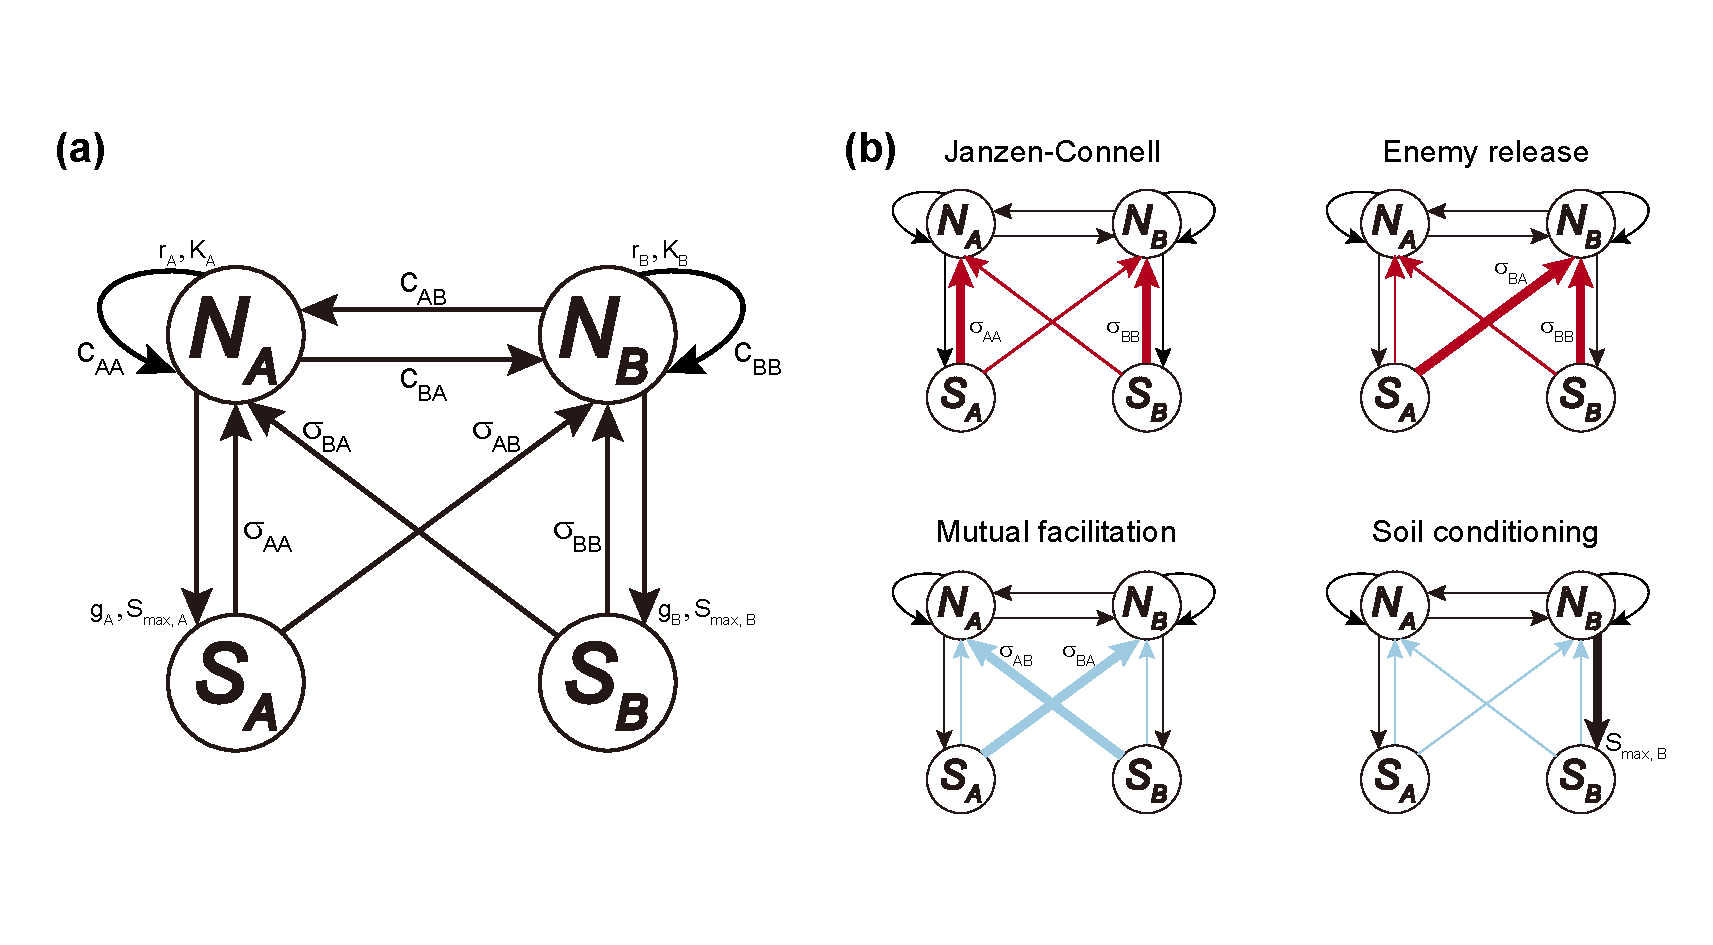
\includegraphics[width=16cm]{Chapter4/ModelFramework4_color_Revised2.pdf}}
	\caption[Conceptual framework for the plant--soil microbe interaction model.]
		{\hspace{1mm}Conceptual framework for the plant--soil microbe interaction model. (a) The model describes the dynamics of two plants (\textit{$N_{A}$} and \textit{$N_{B}$}) and the total density of their associated soil microbial communities (\textit{$S_{A}$} and \textit{$S_{B}$}), considering both plant--plant competition ($c_{ij}$) and plant--soil microbe interaction ($\sigma_{ij}$).  All arrows are labeled with corresponding model parameters; see main text for parameter definitions. (b) The four interaction scenarios analyzed in this study: Janzen--Connell (top left, varying $\sigma_{AA}$ and $\sigma_{BB}$); enemy release (top right, varying $\sigma_{BA}$ and $\sigma_{BB}$); mutual facilitation (bottom left, varying $\sigma_{AB}$ and  $\sigma_{BA}$); and differential soil conditioning (bottom right, varying $\phi_{B}$). Parameters varied in each scenario are highlighted with thick arrows. Soil microbial effects in the Janzen--Connell and enemy release scenario are pathogenic ($\sigma_{ij}<0$, dark red arrows), whereas in the mutual facilitation and differential soil conditioning scenario they are mutualistic ($\sigma_{ij}>0$, light blue arrows). Default parameter values are provided in Appendix C.4 (Table~\ref{table:Parameters}).}
	\label{fig:Framework}
\end{figure}



\clearpage
\begin{figure}[h!]
	\centering
	\makebox[\textwidth][c]{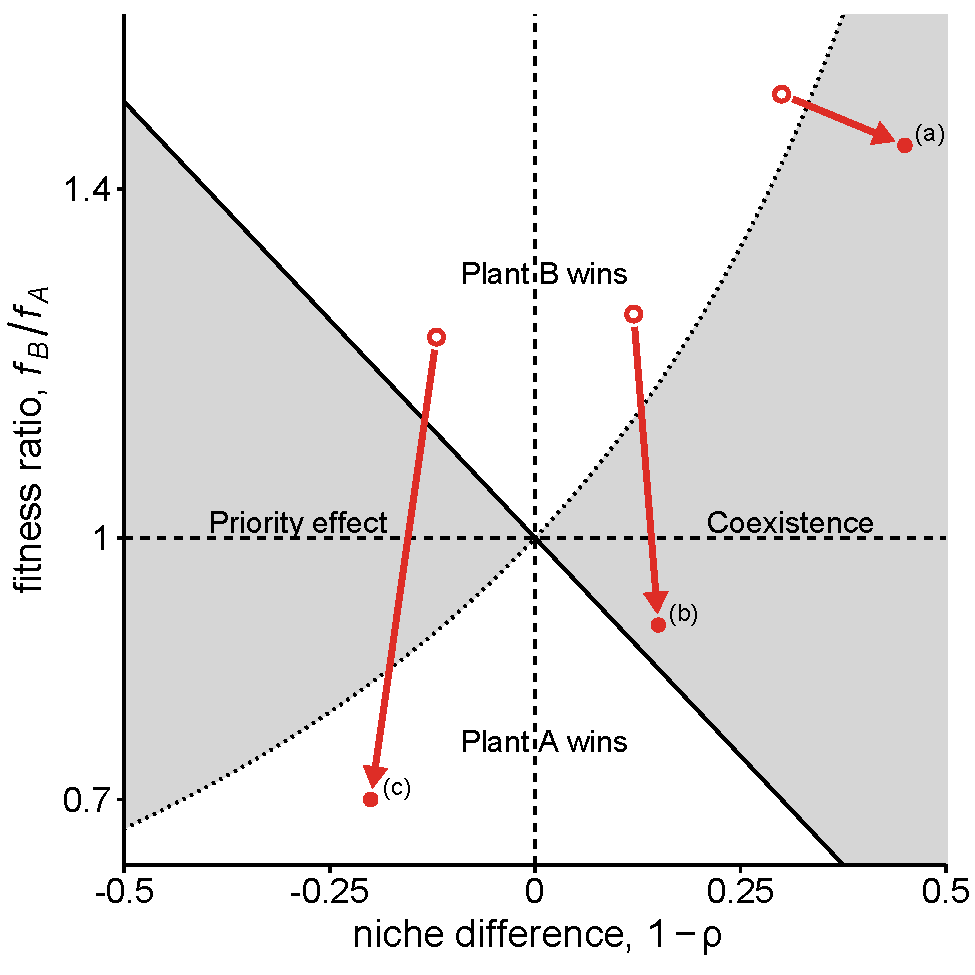
\includegraphics[width=11cm]{Chapter4/Conceptual2.pdf}}
	\caption[Potential effects of soil microbes on the outcome of plant competition, visualized on the parameter space of niche difference and fitness ratio.]
		{\hspace{1mm}Potential effects of soil microbes on the outcome of plant competition, visualized on the parameter space of niche difference ($1 - \rho$, x-axis) and fitness ratio ($f_{B}/f_{A}$, y-axis). The solid and dotted line represent the boundary where $f_{B}/f_{A}$ equals $\rho$ and $1/\rho$, respectively. The right and left gray shaded areas indicate the regions where coexistence and priority effects occur, respectively; the top and bottom white areas indicate where plant B or A is dominant, respectively. The red arrows demonstrate how soil microbes may alter the outcome of competition by (a) acting primarily as a stabilizing mechanism, (b) acting primarily as an equalizing mechanism, or (c) changing the identity of the dominant competitor. Open and solid circles represent competition in the absence and presence of soil microbes, respectively. This visualization was also used for the rest of our simulation results.}
	\label{fig:PopChessonSpace}
\end{figure}



\clearpage
\begin{figure}[h!]
	\centering
	\makebox[\textwidth][c]{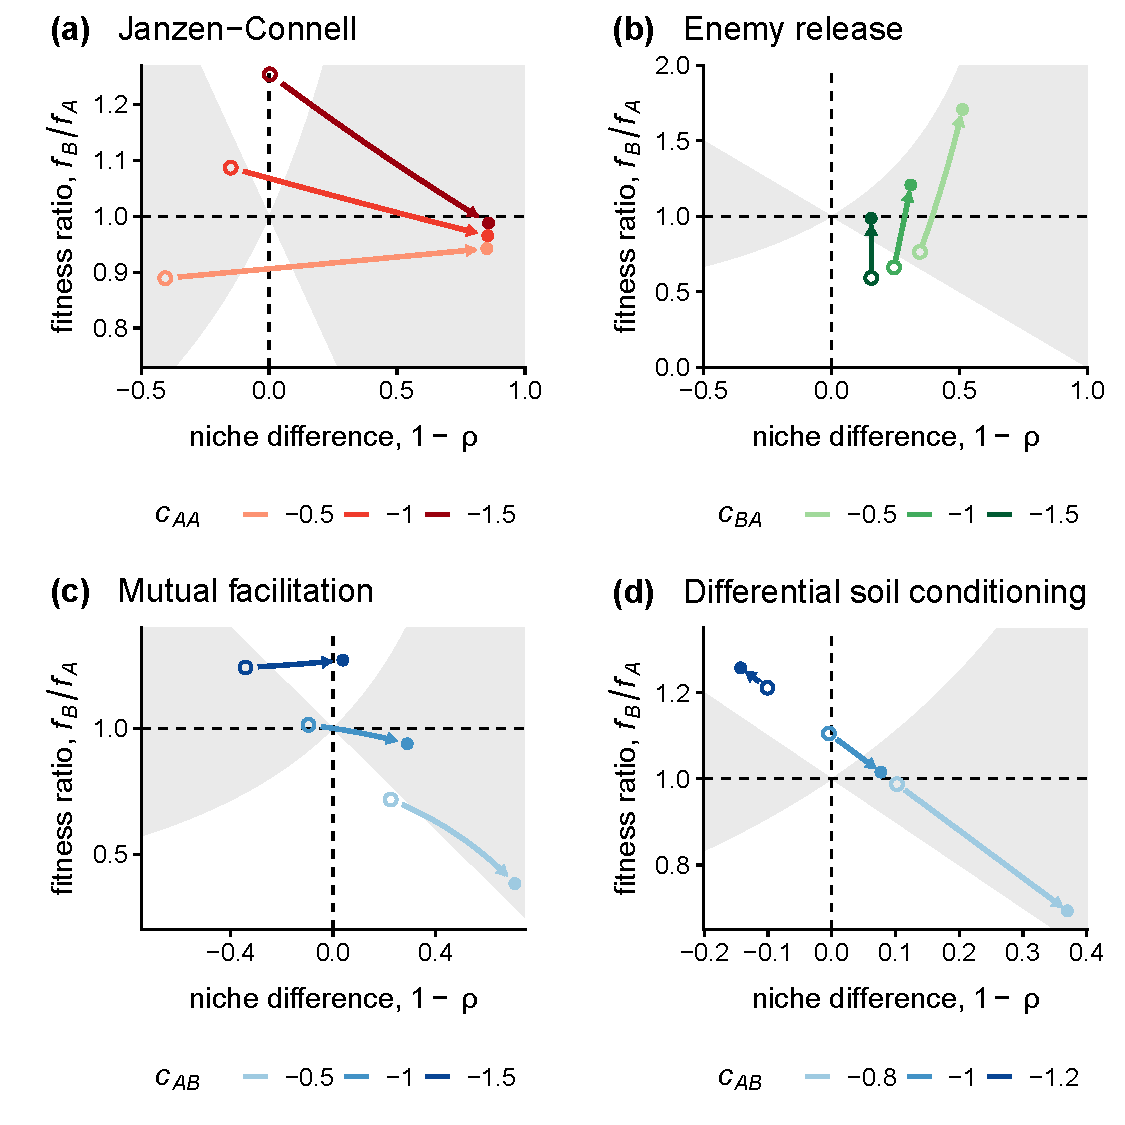
\includegraphics[width=14cm]{Chapter4/Translated_All_together.pdf}}
	\caption[Examples of how plant--soil microbe interactions and plant--plant competition together determine competition outcome.]
		{\hspace{1mm}Examples of how plant--soil microbe interactions and plant--plant competition together determine competition outcome. Four plant--soil microbe interaction scenarios were considered: (a) Janzen--Connell (varying $\sigma_{AA}$ and $\sigma_{BB}$), (b) enemy release (varying $\sigma_{BA}$ and $\sigma_{BB}$), (c) mutual facilitation (varying $\sigma_{AB}$ and  $\sigma_{BA}$), and (d) differential soil conditioning (varying $\phi_{B}$). For each scenario, arrows show how niche difference ($1 - \rho$, x-axis) and fitness ratio ($f_{B}/f_{A}$, y-axis) changed as we varied the strength of soil microbial effects ($\sigma_{ij}$) from weakest (open circles) to strongest (solid circles). To demonstrate its interactive effect with plant--plant competition, this trajectory is shown for different strengths of plant--plant competition ($c_{ij}$) ranging from weak (light colors) to strong (dark colors). Plant--plant competition coefficients that were shown here for each scenario are: (a) $c_{AA}$; (b) $c_{BA}$; (c) $c_{AB}$; and (d) $c_{AB}$. See Appendix C.4 for other plant--plant competition coefficients (Fig.~\ref{fig:Janzen_Connell_everything}--\ref{fig:Soil_Conditioning_everything}) and default parameter values (Table~\ref{table:Parameters}).}
	\label{fig:Scenario_Battleaxes}
\end{figure}



\clearpage
\begin{figure}[h!]
	\centering
	\makebox[\textwidth][c]{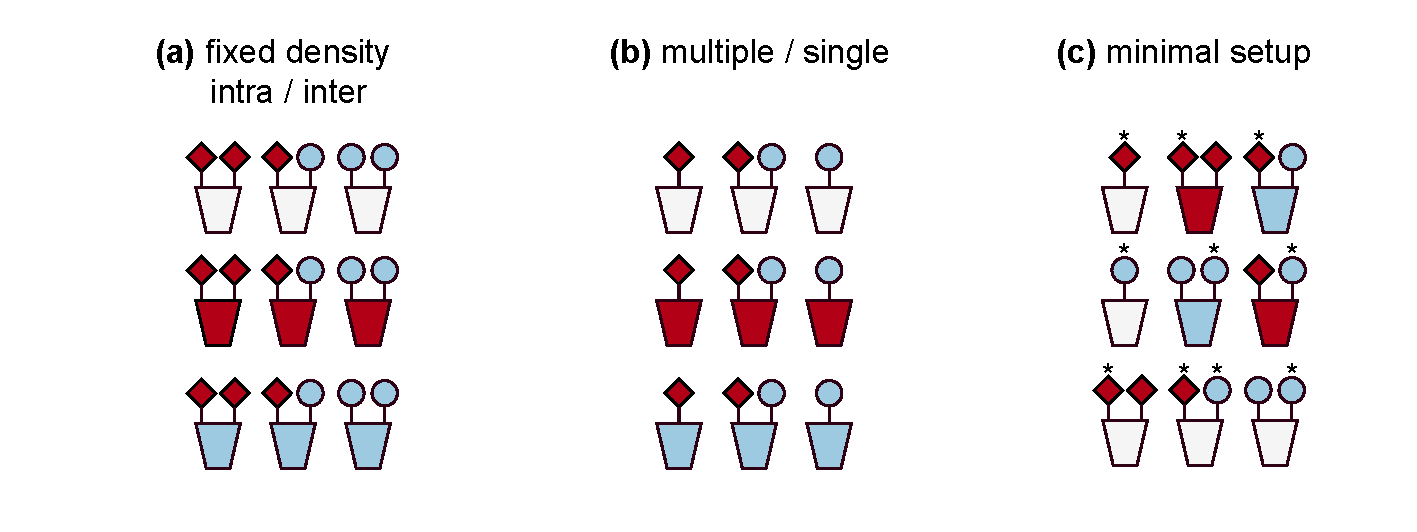
\includegraphics[width=16cm]{Chapter4/ExperimentSetupSmall_OnlyPots_Revised2_starred.pdf}}
	\caption[Experimental designs to quantify the effects of soil microbes on plant competitive outcome.]
		{\hspace{1mm}Experimental designs to quantify the effects of soil microbes on plant competitive outcome. (a) fixed-density intra/inter designs consisting of growing the focal plant in either intra- or inter-specific plant--plant competition; (b) multiple/single designs consisting of growing the focal plant either with or without interspecific plant--plant competition; (c) minimal experimental setup. Pots with different colors represent soils with different conditioning history: no conditioning history or sterile soil (white); conditioned by the diamond plant (dark red); conditioned by the circle plant (light blue). In the minimal setup, competition coefficients can be calculated from measurements of the plants marked with asterisks.}
	\label{fig:ExperimentSetup}
\end{figure}



\clearpage
\begin{figure}[h!]
	\centering
	\makebox[\textwidth][c]{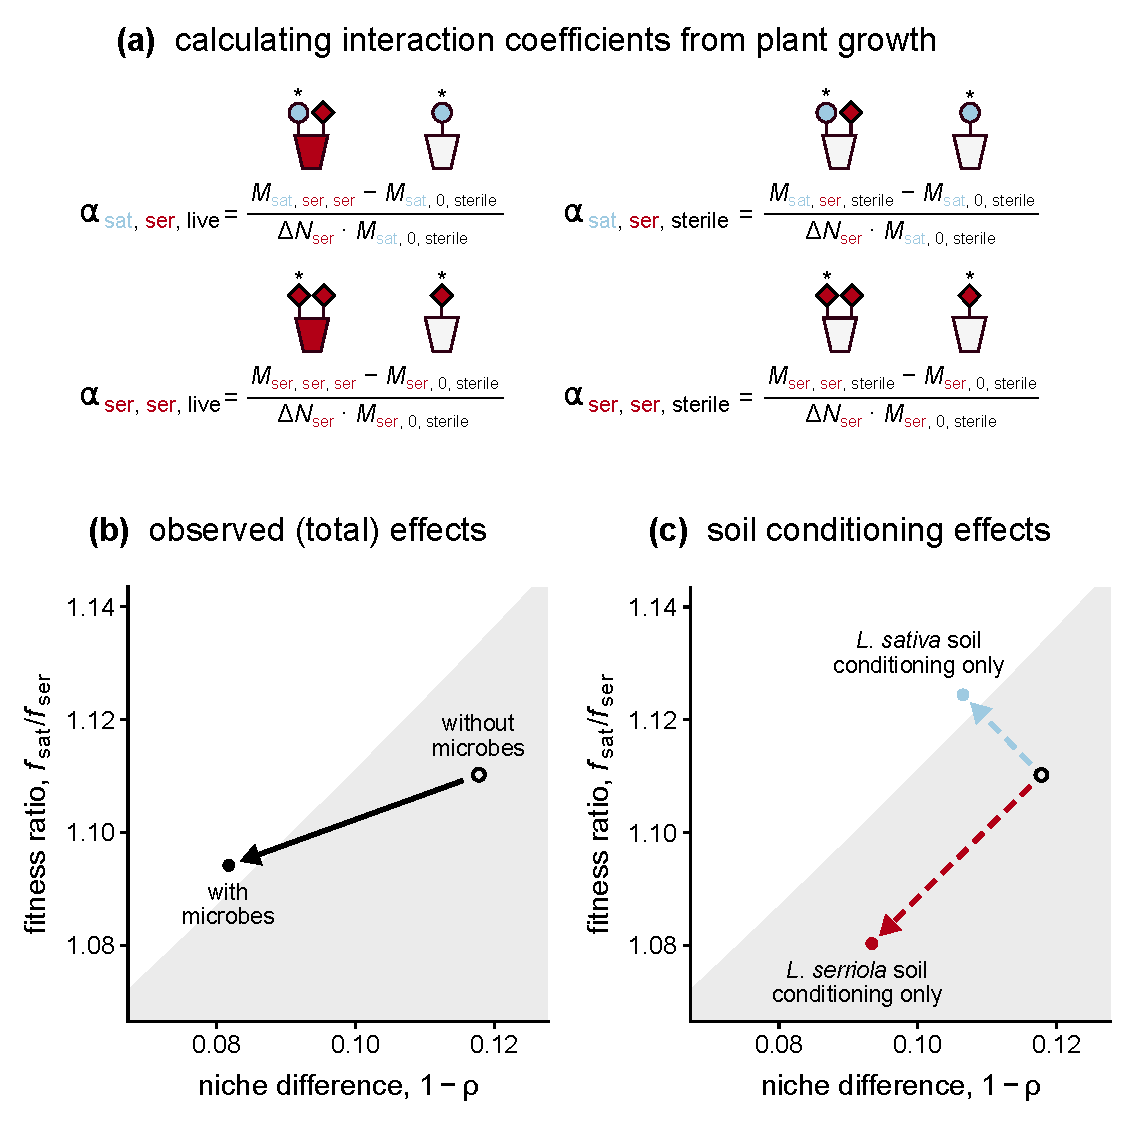
\includegraphics[width=15cm]{Chapter4/Aguilera_2panel_calculations_soil.pdf}}
	\caption[Applying modern coexistence theory to understand the effects of soil microbes on plant competitive outcome using data from \citet{Aguilera2017}as a case study.]
		{\hspace{1mm}Applying modern coexistence theory to understand the effects of soil microbes on plant competitive outcome using data from \citet{Aguilera2017}as a case study. (a) Calculating the competition coefficients representing the sensitivity of \textit{Lactuca sativa} (sat; blue) and \textit{Lactuca serriola} (ser; red) to \textit{L. serriola} in live and sterile soil. $M_{i,j,k}$ represents the biomass of species $i$ competing with species $j$ in soil cultivated by species $k$  (with $0$ indicating no competitor or no soil inoculum); $\Delta N_j$ represents the density of competitors of species $j$. Above each biomass term, we illustrate the corresponding experimental treatment and mark the measured individual with an asterisk. (b) Predicted effect of soil microbes (open circles: microbes absent; solid circles: microbes present) on the outcome of competition between \textit{L. sativa} and \textit{L. serriola}. Using competition coefficients calculated from empirical data, we applied our model to calculate niche difference and fitness ratio (see Box 2). The white region (upper left) indicates that \textit{L. sativa} outcompetes \textit{L. serriola}, whereas the gray region (lower right) indicates coexistence.}
	\label{fig:Aguilera2017Data}
\end{figure}



\clearpage 
\begin{flushleft}
\textbf{Box 4.1}
\end{flushleft}
\begin{infobox}[Separating the stabilizing and equalizing components]

To calculate the components of modern coexistence theory, we applied separation of timescales by assuming that soil microbe dynamics were sufficiently fast compared to plant population dynamics and that all dynamics occurred near equilibrium. In particular, this means that soil microbes reach their plant-determined carrying capacities without any time lag, and die instantly when the host plant dies. Under these conditions, we reduced our model (Eqns.~\ref{eq:SoilA}-\ref{eq:Nb}) to a two-species Lotka--Volterra model (see Appendix C.2), with the following interaction coefficients:

\begin{equation}
\alpha_{ij} = c_{ij} + \sigma_{ij}\phi_{j} .
\tag{4.5}\label{eq:alpha}
\end{equation}

Here, $\alpha_{ij}$ represents the net competitive effect of species $j$ on $i$ and $i$ and $j = A$ or $B$. Importantly, we can observe that net competition consists of two terms: (1) plant--plant competition not related to soil microbes, $c_{ij}$, and (2) soil microbial effects, summarized as $\sigma_{ij}\phi_{j}$.
We assumed plant--plant interactions are competitive ($c_{ij} < 0$) and plant--soil microbe interactions can be either detrimental ($\sigma_{ij} < 0$) or beneficial ($\sigma_{ij} > 0$). Note that when microbes have no effect on plants ($\sigma_{ij}$ or $\phi_{i} = 0$), the model simplifies to pure Lotka--Volterra competition. In addition, if the soil microbes have a very strong positive effect, $\alpha_{ij}$ becomes greater than zero and the plant populations grow towards infinite population size without other regulatory forces.
\par


% Separating ND and FD from the PSF model -- Using Chesson's formula
After transforming the model, we quantified niche overlap and fitness ratio between the two plants using formulas derived specifically for two-species Lotka--Volterra models \citep{Chesson1990, Chesson2008b, Chesson2013ecosys}. Under this formalization, stabilizing mechanisms represent processes that decrease niche overlap ($\rho$, or increase niche difference, $1-\rho$). Here, $\rho$ is the magnitude of difference in inter- to intra-specific interaction coefficients, i.e., $\rho = \sqrt{\frac{\alpha_{BA}\alpha_{AB}}{\alpha_{AA}\alpha_{BB}}}$. Equalizing mechanisms, on the other hand, represent processes that reduce the fitness ratio, which is defined as $\frac{f_{B}}{f_{A}} = \sqrt{\frac{\alpha_{AA}\alpha_{AB}}{\alpha_{BB}\alpha_{BA}}}$. Following these definitions, we derived the niche overlap and fitness ratio between $N_{A}$ and $N_{B}$ as:
\begin{equation}
\rho = \sqrt{\frac{\left ( c_{BA} + \sigma_{BA}\phi_{A} \right )
				   \left ( c_{AB} + \sigma_{AB}\phi_{B} \right )}
				  {\left ( c_{AA} + \sigma_{AA}\phi_{A} \right )
				   \left ( c_{BB} + \sigma_{BB}\phi_{B} \right )}}
\tag{4.6}\label{eq:ND}
\end{equation}
\begin{equation}
\frac{f_{B}}{f_{A}} = \sqrt{\frac{\left ( c_{AA} + \sigma_{AA}\phi_{A} \right )
								  \left ( c_{AB} + \sigma_{AB}\phi_{B} \right )}
								 {\left ( c_{BB} + \sigma_{BB}\phi_{B} \right )
								  \left ( c_{BA} + \sigma_{BA}\phi_{A} \right )}} .
\tag{4.7}\label{eq:FR}
\end{equation}
\end{infobox}



\clearpage
\begin{flushleft}
	\textbf{Box 4.2}
\end{flushleft}
\begin{infobox}[Visualizing the niche difference--fitness ratio parameter space]

In this study, we visualize our simulation results on the parameter space defined by the niche difference ($1-\rho$) and fitness ratio ($f_{B} / f_{A}$) between the two species. Here, we use figure~\ref{fig:PopChessonSpace} as an illustrative example to demonstrate how to interpret our results. The solid linear and dotted curvilinear black lines denote the boundary where fitness ratio is equal to niche overlap ($\rho$) and the inverse of niche overlap ($1 / \rho$), respectively. These two boundaries partition the parameter space into four distinct regions, representing different outcomes of competition. If the two species differ too greatly in fitness relative to their niche difference, one species outcompetes the other (upper and lower white regions). When the niche difference is positive, stable coexistence occurs if the fitness ratio is not too extreme (right gray region). When niche difference is negative, priority effects may occur (left gray region), where community composition depends on which plant arrives first \citep{Mordecai2011, KeLetten2018}.
\par


The pathways shown in Figure~\ref{fig:PopChessonSpace} illustrate how soil microbes might alter competitive outcomes. For example, soil microbes may promote coexistence by primarily affecting niche difference (a stabilizing mechanism, arrow a in Fig.~\ref{fig:PopChessonSpace}) or fitness ratio (an equalizing mechanism, arrow b Fig.~\ref{fig:PopChessonSpace}). Soil microbes may also flip the competitive hierarchy by changing the identity of the dominant competitor (arrow c in Fig.~\ref{fig:PopChessonSpace}).
Note that since microbe-mediated parameters make up part of the phenomenological interaction coefficients (Eqn.~\ref{eq:alpha}), varying their strength would simultaneously affect both niche difference and fitness ratio.
The only exception being the special case where a pair of $\sigma_{ij}$ varied in a way that maintained the value of either Eqns.~\ref{eq:ND} or \ref{eq:FR}.
In general, however, plant--soil interactions would predominantly affect either the stabilizing or equalizing components depending on the specific interaction network between plants and soil microbes (see section \textit{Synthesizing microbial effects on plant coexistence}).
\end{infobox}
\chapter{Testing chronosequence predictions with longitudinal data reveals microbial community convergence}
%\chaptermark{Positive frequency-dependence}
%\renewcommand{\sectionmark}[1]{}
\fancyhead[LE, RO]{\thepage}
\fancyhead[RE]{CHAPTER 5}
\fancyhead[LO]{TESTING CHRONOSEQUENCE WITH LONGITUDINAL DATA}
\fancyfoot{}
\renewcommand{\headrulewidth}{0pt}
\setlength{\parindent}{1cm}



\begin{comment}
\documentclass[hidelinks,letterpaper, 11pt]{article}
\usepackage{graphicx, bm, booktabs, lineno, array}
\usepackage[fleqn]{amsmath}
\usepackage{nicefrac}
\usepackage[compress,comma]{natbib}
\usepackage[right=1in, left=1in, top=1in, bottom=1in]{geometry}
\usepackage[parfill]{parskip}
\usepackage[usenames,dvipsnames]{color}
\usepackage[font=large,labelfont=bf,margin=1cm, labelsep = none]{caption} % caption formatting
\usepackage{setspace}
\usepackage{gensymb}
\usepackage{color}
\usepackage{sidecap}
%\usepackage{floatrow}
\usepackage{etoolbox}
\usepackage{tcolorbox}
\usepackage{newpxtext,newpxmath}
\tcbuselibrary{breakable}
%\usepackage{indentfirst}
\newbool{MyRefNumbers}
\usepackage{authblk}
\usepackage{hyperref}
\usepackage{mathpazo}
\usepackage[color=cyan, textsize=tiny]{todonotes}
\usepackage[font={normalsize}]{caption}
\usepackage{adjustbox}
\usepackage{array}
\usepackage{booktabs}
\usepackage{multirow}
\usepackage{tabularx}
% \usepackage{titling}

\setlength{\mathindent}{0pt}
\setlength{\parindent}{1cm}
% \makeatletter
% \makeatother
\pdfminorversion=3

% For table
\newenvironment{myindentpar}[1]%
{\begin{list}{}%
		{\setlength{\leftmargin}{#1}}%
		\item[]%
	}
	{\end{list}}
\newcommand*\samethanks[1][\value{footnote}]{\footnotemark[#1]}
\newcommand\blfootnote[1]{%
	\begingroup
	\renewcommand\thefootnote{}\footnote{#1}%
	\addtocounter{footnote}{-1}%
	\endgroup
}
\newcommand{+}{\raisebox{.4\height}{\scalebox{.6}{+}}}
\newcommand{\minus}{\raisebox{.4\height}{\scalebox{.8}{-}}}
% Command to recount supplement
\newcommand{\beginsupplement}{%
	\setcounter{table}{0}
	\renewcommand{\thetable}{S\arabic{table}}%
	\setcounter{figure}{0}
	\renewcommand{\thefigure}{S\arabic{figure}}%
}
% Command to center oversized images in floats
\newcommand{\centerfloat}{%
	\parindent \z@
	\leftskip \z@ \@plus 1fil \@minus \textwidth
	\rightskip\leftskip
	\parfillskip \z@skip}
\renewcommand\Affilfont{\fontsize{12}{12}\selectfont}
\newcommand{\ignore}[2]{\hspace{0in}#2}
\end{comment}



\begin{comment}
\begin{document}
	
\doublespacing
\title{Testing chronosequence predictions with longitudinal data reveals microbial community convergence}
\author[1, $\dagger$]{Po-Ju Ke}
\author[1, 2]{J. Nicholas Hendershot}
\author[1, $\dagger$]{Tadashi Fukami}
\affil[1]{Department of Biology, Stanford University, Stanford, California, USA}
\affil[2]{Center for Conservation Biology, Stanford University, Stanford, California, USA}
 
\date{\today}
\maketitle
\blfootnote{$\dagger$ Correspondence author: Department of Biology, Stanford University, Stanford, California 94305-5020, USA. Phone: +1 650-721-1711. Fax: +1 650-723-6132. Email: pojuke@stanford.edu, fukamit@stanford.edu}
	
\onehalfspacing
\noindent \textbf{Running title:} Predicting community structure with chronosequence\\
\noindent \textbf{Keywords:} beta diversity, \textit{Carpobrotus edulis}, community assembly, sand dunes, space-for-time substitution, succession\\
\noindent \textbf{Type of article:} Research article
	
\begin{myindentpar}{1cm}
	\textbf{Words in Abstract:} $\sim$ 200\\
	\textbf{Words in main text:} $\sim$ XXX\\
	\textbf{Number of references:} $\sim$ 50\\
	\textbf{Number of figures:} 5\\
\end{myindentpar}
	
\noindent \textbf{Authorship statement:} PJK and TF conceived the study; PJK conducted the study; PJK and JNH analyzed the data; PJK wrote the first draft of the manuscript with substantial contribution from all authors.\\
	
\noindent \textbf{Data accessibility statement:} Should the manuscript be accepted, all data and computer scripts supporting the results will be archived in a public repository, with the DOI included in the article.\\

\linenumbers
\doublespacing
\end{comment}



\section{Abstract}
Chronosequences, defined as a series of sites that differ in the time since their initiation, are commonly used for studying ecological succession, but the usefulness of chronosequences has been controversial. Here, we show how chronosequence inferences can be strengthened by short-term longitudinal data.
Focusing on soil fungi associated with two coastal plants, the ice plant (\textit{Carpobrotus edulis}) and the yellow bush lupine (\textit{Lupinus arboreus}), we characterized fungal communities associated with plant individuals along a plant age chronosequence. 
We then used these data to predict the composition of fungal communities and evaluated the predictions by re-sampling a subset of individuals annually for another two years.
We found that the beta diversity of fungal communities across host plants decreased with plant age. Fungal communities exhibited a consistent compositional shift across the three sampling years, and we were able to predict their composition more accurately as plants aged. Together, the two data types strengthened inference of a deterministic process shaping the fungal communities. Our results demonstrate how a combined approach can provide a more robust understanding of the processes shaping ecological succession.
\medskip


\textbf{Keywords:} beta diversity, \textit{Carpobrotus edulis}, community assembly, sand dunes, space-for-time substitution, succession



\section{Introduction}
Ecological communities may converge towards a common structure or diverge because of temporally contingent factors \citep{Fukami2005, DiniAndreote2015, Meiners2015, Clark2019}.
% Predicting successional dynamics has been a central theme of community ecology \citep{DiniAndreote2015, Meiners2015}.
% Classic viewpoint suggests that communities would converge towards a common structure as succession unfolds through time \citep{ConnellSlatyer1977}, whereas recent studies have also highlighted the role of stochasticity and other contingent factors in causing community divergence \citep{DiniAndreote2015, Clark2019}. 
% Nevertheless, elucidating how community trajectories and the underlying mechanisms develop through time remains challenging. 
Predicting which happens in which instances of succession remains challenging because long-term longitudinal data are scarce (but see \citealp{Li2016}), leading to a frequent reliance on chronosequences (i.e., sequences constructed from a series of sites differing in the time since they were formed, \citealp{Walker2010}). 
The utility of chronosequences for inferring community convergence and divergence has been controversial since factors that influence convergence and divergence may change during succession \citep{Johnson2008, Damgaard2019}.
% The assumption of space-for-time substitution behind the chronosequence approach implies that sites of different ages traced the same developmental history.
% However, the utility of chronosequences for inferring temporal dynamics has been questioned, particularly if abiotic and biotic conditions did not remain constant over the time span of the successional change under study \citep{Johnson2008, Damgaard2019}.
One way to strengthen the chronosequence approach is to supplement it with short-term longitudinal data \citep{Damgaard2019}. The assumption that different sites have followed the same history can be tested by repeatedly sampling the chronosequence.
Studies that took this approach showed that chronosequences could accurately predict the temporal changes in ecosystem-level consequences of succession, such as soil formation and biomass accumulation \citep{vanbreugel2006, Lebrijatrejos2010, Walker2010}.
However, it is unclear how accurate chronosequences may be in describing changes in more detailed community structure, such as species composition \citep{Foster2000, Mora2015, Rolo2016}.
% However, when focusing on more detailed community-level properties, such as species richness and community composition, sites that composed the chronosequence may follow different successional trajectories \citep{Foster2000, Mora2015, Rolo2016}. 
% Therefore, when studying whether communities converge or diverge during ecological succession, comprehensive integration of both chronosequence and longitudinal data is necessary for correct inference of the underlying processes.
\par


% Study aims and discuss why soil communities are a great study system
In this study, we combine chronosequence and short-term longitudinal observation to investigate the compositional changes during the succession of plant-associated soil fungal communities.
Using microbial communities to test theories of succession has the advantage that succession occurs at manageable time scales \citep{Fierer2010, Chaparro2013, Gao2019}, therefore allowing the application of our combined approach.
The succession of soil microbial communities, in particular, represents an ideal system to test for community convergence or divergence as plants and other geological processes continuously affect the soil microbial community \citep{BrownJumpponen2014, Castle2016, Dinnage2019}. Although the primary succession of soil microbial communities has been investigated across long time frames of soil development (e.g., \citealp{BrownJumpponen2014, Castle2016}), studies on their fine-scale successional patterns in natural systems are rare. 
\par


% Study approaches
We used a series of high-resolution aerial photos of the coastal dune vegetation at Bodega Bay (California, USA) to construct a chronosequence.
We estimated the age of individual plants and used it as a proxy of the successional stage of their associated soil fungal community. By collecting soil from plant individuals of different ages, and re-sampling a subset of these individuals for another two years, we tested if the two approaches showed similar patterns of community convergence or divergence. From the chronosequence data, we predicted that compositional variation among fungal communities would decrease with the age of their host plant as a result of a deterministic selection force. If the chronosequence correctly captured relevant ecological processes, we should be able to predict the fungal community composition more accurately as plants aged. 
% Our longitudinal data indicated this to be the case.
\bigskip



\section{Methods}
\subsection*{Study system}
% General background of the sytem site
We conducted our field sampling at the coastal foredunes of Bodega Bay, California, USA (38$^{\circ}$19$^\prime$ N, 123$^{\circ}$3$^\prime$ W), located within the Unuversity of California Davis Bodega Marine Reserve and the Sonoma Coast State Beaches. Bodega Bay experiences a Mediterranean-type climate, with an average temperature of 15.8$^{\circ}$C and annual precipitation of 790 mm that occurs mostly between November to April \citep{Conser2009}. 
\par


% General information of the two plants
We focused on the soil fungal community associated with two dominant species at Bodega Bay: ice plant \textit{Carpobrotus edulis} (Aizoaceae) and yellow bush lupine \textit{Lupinus arboreus} (Fabaceae).
\textit{C. edulis} is a south African succulent perennial that was introduced to California for erosion control, but has since invaded California coastal dunes extensively. The plant has a prostrated growth form and, with branches growing over one another, forms thick layers of recalcitrant litter mats up to 40 cm in depth \citep{DAntonio1990}. \textit{C. edulis} alters both biotic \citep{delaPena2010} and abiotic soil properties (e.g., increase soil organic content but decreases soil pH), resulting in growth suppression of other species even after its removal \citep{Conser2009, Novoa2013, Novoa2014}.
\textit{L. arboreus}, is a fast-growing nitrogen-fixing shrub native to central California coastal grassland and dunes. Nitrogen fixation by \textit{L. arboreus} enriches the nutrient-poor sandy soils and facilitates the growth of non-native grasses \citep{Maron1996, Maron2001}. 
\par


%Plant individual selection
We used the age of host plant individuals as a proxy of the successional stage of the soil microbial communities. 
Using a series of aerial photos that were taken annually at Bodega Bay from 1992 to 2016 \citep{Danin1998}, plant ages were estimated by identifying the first year when the individual appeared in the photos. 
We were able to identify individuals to the species level and estimate their age because the foredune vegetation is relatively simple, with low coverage and little vertical structure.
With our age (i.e., successional stage) estimations, we constructed a chronosequence of soil microbial community development at the individual plant level. For the two plant species, we selected 60 individuals from our chronosequence that differed in their age, ranging between 2 to 25 years for \textit{C. edulis} and between 1 to 11 years for \textit{L. arboreus}. 
\par



\subsection*{Soil sampling}
%Soil sampling for microbial community patterns
In July 2015 we collected three soil samples beneath each of the 120 individuals (i.e., 2 species $\times$ 60 individuals). Soil samples were collected roughly on the mid-radius of the plant individual (i.e., midway between the center and the edge of the crown) at three different angles (i.e., azimuth angles 0$^{\circ}$, 120$^{\circ}$, and 240$^{\circ}$). After gently removing the litter that covered the soil surface, we collected soils in separate sterile 50 mL Falcon tubes. 
All soil samples were stored at 4$^{\circ}$C before being processed in the lab. Within one week after collection, each soil sample was passed through a sterile 2 mm mesh sieve, homogenized thoroughly in a sterile plastic bag, and stored at -20$^{\circ}$C. 
The sampling resulted in 360 fungal communities (i.e., 2 species $\times$ 60 individuals $\times$ 3 samples), which were characterized by next-generation sequencing (see section `DNA sequencing of fungal community'). As the fungal communities were collected from plant individuals along the chronosequence, we were able to test for fungal community convergence under the assumption of space-for-time substitution.
\par


To validate the successional dynamics predicted by our samples collected in 2015, we revisited the chronosequence in both July 2016 and 2017 and collected soil samples from a subset of our original plant individuals (i.e., 33 individuals for \textit{C. edulis} and 43 for \textit{L. arboreus}). 
We collected three soil samples from each individual following the same procedure. To avoid being confounded by soil disturbance created during the previous field season, soil samples were collected from positions adjacent to the original sampling position in 2015. 
For each species, we also collected soil samples from three randomly selected juveniles, which were defined as individuals that germinated within one year and were too small to be visible on the aerial photos from the previous year. 
Each year, the  234 soil samples (i.e., 70 individuals $\times$ 3 samples + 2 species $\times$ 3 juveniles) were processed, and their fungal communities were characterized using the same methods as in 2015.
\par



\subsection*{DNA sequencing of fungal community}
We prepared the fungal DNA library for each year's samples with the following steps.
Within one month after sampling, we extracted fungal DNA from all soil samples using the PowerSoil DNA Isolation Kit (Qiagen). 
We amplified the fungal internal transcribed spacer 1 region (ITS1) with primer pair ITS1-F$\textunderscore$KYO1 (5$^\prime$- CTH GGT CAT TTA GAG GAA STA A -3$^\prime$) -- ITS2$\textunderscore$KYO2 (5$^\prime$- TTY RCT RCG TTC TTC ATC -3$^\prime$) \citep{Toju2012}. Primers were concatenated with 3 -- 6-mer Ns \citep{Lundberg2013} and an Illumina sequencing primer region, resulting in a fusion primer for our PCR reactions (forward: 5$^\prime$- TCG TCG GCA GCG TCA GAT GTG TAT AAG AGA CAG -- [3--6-mer Ns] -- [ITS1-F$\textunderscore$KYO1] -3$^\prime$; reverse: 5$^\prime$- GTC TCG TGG GCT CGG AGA TGT GTA TAA GAG ACA G -- [3--6-mer Ns] -- [ITS2$\textunderscore$KYO2] -3$^\prime$). 
Our PCR reaction consisted of 3.2 $\mu$L of MQ water, 5 $\mu$L of MyTaq HS DNA polymerase Mastermix (Bioline), 0.4 $\mu$L of each primer (10$\mu$M for both forward and reverse primer), and 1 $\mu$L of extracted DNA (total volume 10 $\mu$L). PCR reactions were run with a hot start at 95$^{\circ}$C for 2 min, followed by 36 cycles of 95$^{\circ}$C for 20 sec, 50$^{\circ}$C for 20 sec, 72$^{\circ}$C for 50 sec, and a final extension at 72$^{\circ}$C for 10 min. We set a 1$^{\circ}$C/s ramp rate to prevent chimeric amplicon generation. 
After this first PCR process, a subsequent second PCR was run to add sample-specific tags. The fusion primers used in this second PCR concatenates P5/P7 Illumina adaptors, 8-mer index sequences, and the sequencing adaptor \citep{Hamady2008} (forward: 5$^\prime$- AAT GAT ACG GCG ACC ACC GAG ATC TAC AC -- [8-mer tag] -- TCG TCG GCA GCG TC -3$^\prime$; reverse: 5$^\prime$- CAA GCA GAA GAC GGC ATA CGA GAT -- [8-mer tag] -- GTC TCG TGG GCT CGG -3$^\prime$). The second PCR consisted of 8 cycles with the same temperature profile as our first PCR but with an annealing temperature of 50$^{\circ}$C. 
After PCR, we purified the product using the AMPure XP Kit (Agencourt), with a sample : bead ratio of 1 : 0.6. Finally, we pooled 5$\mu$L of normalized PCR product from each sample to create a pooled library for samples collected at that year. 
Libraries were stored at -80$^{\circ}$C and later pulled together based on their Qubit reads after the library for 2017 samples was prepared in November 2017.
The final pooled library, consisting of fungal DNA from samples collected across all three years, was sequenced using the Illumina MiSeq sequencer of the Stanford Functional Genomics Facility (2 $\times$ 250 cycle sequencing kit) with 15$\%$ PhiX spike-in.
\par


We processed the Illumina MiSeq sequencing reads with the Claident pipeline (\citealp{Tanabe2013}, v0.2.2015.11.19). We converted raw Miseq BCL data to FASTQ data with the program bcl2fastq v1.8.4. We then demultiplexed the library based on the sample-specific 8-mer index sequences. All sequencing reads with low quality scores ($<$ 30) were deleted. The obtained forward and reverse sequencing reads were fused using PEAR v0.9.6 \citep{Zhang2014}, and low-quality merged reads (quality score $<$ 30 or length $<$ 150 bp) and chimeric reads were eliminated using UCHIME v4.2 \citep{Edgar2011}. Sequencing reads that passed through all filtering processes were then clustered into operational taxonomic units (OTUs), based on a 97$\%$ sequence similarity cutoff, using VSEARCH \citep{Rognes2016}. After clustering, fungal OTUs with less than ten total sequencing reads were removed, resulting in a final sample $\times$ OTU matrix. Taxonomy was assigned to the OTUs using the RDP Naive Bayesian rRNA Classifier v2.11 \citep{Wang2007} trained on the Warcup Fungal ITS training set 2 \citep{Deshpande2016} for fungi. Based on the taxonomic assignment results, ITS1 sequences other than those of the fungi kingdom were removed from the dataset, and the remaining OTUs were assigned a trophic mode based on \textit{FUNGuild} \citep{Nguyen2016}.
% Potential contaminant OTUs were identified statistically based on their prevalence in PCR and extraction negative controls (two of each for every 96 well plate reaction) using the R package decontam \citep{Davis2018}.This resulted in the elimination of \ignore{36} XX fungal OTUs. 
% The whole bioinformatics process resulted in \ignore{19,868} XX,XXX OTUs, representing \ignore{1,772,220} X,XXX,XXX ITS1 sequencing reads. 
\par



\subsection*{Data analysis}
% General overview of data analysis and data processing
% We applied both distance-based and model-based analyses to test for convergence of fungal communities during succession.
% As our model-based analysis are based on hierarchical Bayesian approaches (see below, \citep{Ovaskainen2017}), we fitted models by treating each soil sample as separate observation units. On the other hand, we summed the OTU abundances of the three samples that were collected from the same plant individual during the same year to avoid pseudo-replication in the distance-based analysis (i.e., treating plant individuals collected at different years as observation units). 
We summed the OTU abundances of the three samples that were collected from the same plant individual during the same year to avoid pseudo-replication (i.e., treating plant individuals collected at different years as observation units). Individuals that recovered less than three samples from the sequencing run were removed from the following analysis. 
The sample $\times$ OTU table was then rarefied to 1000 sequencing reads per sample (R package phyloseq, \citealp{McMurdie2013}). 
For the following analysis, we focused on fungal OTUs that occurred in more than 20$\%$ of the samples in order to ensure adequate model fit in our model-based analysis (see later for detail). 
% For consistency, the same 20$\%$ frequency constraint was also applied to the distance-based analysis. 
Note that all statistics with plant age as a predictor were performed separately for \textit{C. edulis} and \textit{L. arboreus}. This is because the two species vary in their longevity and thus the same age does not necessarily represent the same life stage.
\par


% Distance-based approach -- NMDS
We first applied a distance-based approach to characterize the overall differences in fungal community composition among plant individuals at different sampling year. 
To visualize the compositional shifts, we further limited our ordination to plant individuals that were sampled at all three years (i.e., age $\tau$, $\tau + 1$, and $\tau + 2$ in 2015, 2016, and 2017, respectively). 
We visualized fungal communities of the remaining 90 \textit{C. edulis} and 120 \textit{L. arboreus} observation units (i.e., plant individual $\times$ year sampled) with non-metric multidimensional scaling (NMDS) based on Bray--Curtis dissimilarity (with R package vegan). We tested for the effects of soil host species identity and plant age with permutational multivariate analysis of variance (PERMANOVA with 999 permutations, \citealp{Anderson2011}). 
On the NMDS plot, we used a vector to connect fungal communities that were collected from the same individual during different sampling years, pointing from the coordinates that represented the 2015 fungal community to that of 2016 and 2017. We quantified the x- and y-components of the vector (i.e., $\Delta$NMDS 1 and $\Delta$NMDS 2), which represent the overall direction and magnitude of community shifts. In particular, vectors that moved toward similar direction indicate a consistent compositional shift of fungal communities over succession.
\par


% Distance-based approach -- Spatial beta
Fungal communities collected along the chronosequence allowed us to test for the spatial signature of community convergence. Namely, if fungal communities were converging over succession, their dissimilarity would decrease with plant age class. 
For each species, we used the data from all 60 plant individuals collected in 2015 and calculated the beta diversity among fungal communities associated with plant individuals of the same age class. Beta diversity for each age class was calculated as the distance of fungal communities to the centroid of each age class.
% We also calculated beta deviation following \citep{Tello2015, Vannette2017}. The purpose is to compare the observed level of beta diversity in each age class to those expected if communities were assembled randomly within the constraints imposed by the observed species abundance distributions.
We then fitted linear models to quantify how beta diversity varied with increasing plant age.
As beta diversity was not meaningful for age classes with only one individual (i.e., distance to centroid within the age class would be zero), we deleted these communities when fitting linear models. 
We also visualized the trend in beta diversity with increasing plant individual age with a three-year moving window (i.e., the centroid was calculated using fungal communities associated with age $\tau - 1$, $\tau$, and $\tau + 1$ individuals).
\par


% Model-based approach -- HMSC
We also tested for community convergence using the re-sampling data that we collected in 2016 and 2017 via repeatedly sampling a subset of the plant individuals. 
For this analysis, we turned to a model-based approach with the R package HMSC \citep{Ovaskainen2017}, which is able to capture OTU-specific temporal patterns and generate predictions of the community composition. 
% Different from the previous ordination approaches, this model fitting were performed by treating each soil sample as separate observation units in order to take advantage of the hierarchical Bayesian approach implemented in \textit{HMSC} \citep{Ovaskainen2017}. 
To predict fungal OTU abundances, we fitted models with plant age as fixed effect and plant individual as random effect on a training set, which consisted of data from all 60 plant individuals collected in 2015. The abundance of fungal OTUs were assumed to follow an over-dispersed Poisson distribution to account for changes in the mean--variance relationship inherent with microbial count data. For all models, the MCMC sampling was conducted for 1,000,000 iterations, with a burn-in phase of 500,000 iterations and thinned every 100 iterations. 
After fitting the model, we used data collected from 2016 and 2017 as separate test sets to see if the predictability of fungal communities varied with plant age. 
In particular, we quantified the Bray--Curtis dissimilarity between the predicted and observed fungal community composition (i.e., age $\tau + 1$ and $\tau + 2$ in 2016 and 2017, respectively) and then assessed its relationship with plant age by fitting linear models. 
% The relationship between the Bray--Curtis dissimilarity and plant age in 2015 (i.e., age $\tau$) was assessed with the R package glmmTMB, assuming that the dissimilarity metric followed a beta distribution). If dissimilarities decreased with plant age, we would conclude that the communities are converging over succession since the predictability of the fungal community composition increased. 
If the Bray--Curtis dissimilarity decreased with plant age, we concluded that the communities are converging over succession since the predictability of the fungal community composition increased. 
% To assess the robustness of the community convergence pattern, we also fitted additional models for common OTUs (i.e., those that occurred in more than 50$\%$ of the samples) and at different taxonomic resolution (i.e., by aggregating OTUs based on assigned taxonomy, ranging from Phylum to Genus).
\par



\section{Results}
% Distance-based approach -- NMDS
Fungal composition changed across the three sampling years, mainly captured by the NMDS 2 axis, whereas the effect of host species was represented by the NMDS 1 axis (Fig.~\ref{fig:3YrNMDS_Individual}; PERMANOVA, species effect: $R^{2}=0.13$; age effect for \textit{C. edulis}: $R^{2}=0.06$; \textit{L. arboreus}: $R^{2}=0.05$; all $P<0.001$).  
Most fungal communities exhibited a consistent compositional shift across the three sampling years. Fungal communities associated with the same individual showed an upward movement along the NMDS 2 axis, but inconsistent movement in NMDS 1 (Figs~\ref{fig:FourQuadrate_Individual_Species} and \ref{fig:FourQuadrate_Individual_Species_SI}).
The yearly compositional shifts were larger for \textit{L. arboreus} compared to \textit{C. edulis}, as indicated by the ellipses in Figure~\ref{fig:3YrNMDS_Individual} and the higher proportion of upward movement in Figure~\ref{fig:FourQuadrate_Individual_Species}.
% See also Figs~\ref{fig:3YrNMDS_Sample} and \ref{fig:FourQuadrate_Sample_Species} for similar patterns when separate soil samples, instead of plant individuals, were plotted as units of replication.
\par


% Distance-based approach -- Spatial beta
For fungal communities collected from plant individuals along the chronosequence in 2015, beta diversity declined significantly with plant age for both \textit{C. edulis} and \textit{L. arboreus} (Fig.~\ref{fig:CombinedFull2015Beta_Individual_SI}; \textit{C. edulis}: Pearson's $r=-0.46$, $P=0.001$; \textit{L. arboreus}:  Pearson's $r=-0.27$, $P=0.04$). Similar trend of beta diversity were observed with a three-year moving window averaging (Fig.~\ref{fig:CombinedFull2015Beta_Individual}).
% However, only the beta deviation of \textit{C. edulis} decreased with plant age (Fig.~\ref{fig:Full2015Beta_Individual}b). 
% See also Figs~\ref{fig:Full2015Beta_Sample} and \ref{fig:MovingWindowBeta_Sample} for similar patterns when soil samples were plotted as units of replication.
\par


% Model-based approach -- HMSC
Bray--Curtis dissimilarity between the model prediction and observed community composition decreased (Figs~\ref{fig:HMSC_Species_Individual_Full2015} and \ref{fig:HMSC_Species_Individual_Full2015_SI}; all $P<0.01$), indicating convergence in fungal species composition
Test sets collected in both 2016 (Fig.~\ref{fig:HMSC_Species_Individual_Full2015}) and 2017 (Fig.~\ref{fig:HMSC_Species_Individual_Full2015_SI}) showed the same convergence pattern (Pearson's $r$ for \textit{C. edulis} in 2016 and 2017: $-0.55$ and $-0.64$; for \textit{L. arboreus} in 2016 and 2017: $-0.36$ and $r=-0.40$; all $P < 0.05$). 
% The results were robust when we fitted models with different fungal taxonomic levels and frequency thresholds.
When inspecting the changes in fungal trophic mode (Fig.~\ref{fig:Funguild_HMSC_Species_Individual_Full2015}), we found that OTUs within a trophic mode exhibited different temporal trends. Moreover, many \textit{L. arboreus}-associated pathotrophic fungi increased significantly through time, whereas those associated with \textit{C. edulis} mostly decreased or increased less significantly (Fig.~\ref{fig:Funguild_HMSC_Species_Individual_Full2015Pathogen}).
% See also Fig.~\ref{fig:HMSC_Species_Sample_Full2015} for similar patterns when plant individuals were plotted as units of replication. 
\par



\section{Discussion}
% Biology of the system -- plant host effects and who's changing? 
By repeatedly sampling the soil fungal community along a chronosequence of soil conditioning by plant individuals, we found multiple pieces of evidence for community convergence (Figs~\ref{fig:FourQuadrate_Individual_Species}--\ref{fig:HMSC_Species_Individual_Full2015}).
At our field site, plant-associated soil fungal communities started to assemble as plants colonize bare sand. 
The plant species that arrived and conditioned the soil affected fungal community assembly, selecting for different species over time (Fig.~\ref{fig:3YrNMDS_Individual}). 
These results indicate that host plants drove the succession of the fungal communities \citep{RoyBolduc2016, Scheublin2004}. This pattern contrasts with previous studies that showed little effect of plant species identity on the primary succession of soil microbes \citep{BrownJumpponen2014, Sikes2014}.
With our model-based approach, we found that the abundance of many pathotrophic fungi increased through time when associated with \textit{L. arboreus}, whereas pathotrophic fungi associated with \textit{C. edulis} either decreased or increased to a lesser extent (Fig.~\ref{fig:Funguild_HMSC_Species_Individual_Full2015Pathogen}).
This result might indicate a release from soil-borne enemies of the introduced \textit{C. edulis} \citep{Keane2002, Callaway2004}, and that pathotrophic fungi at Bodega Bay are better at forming associations with the native \textit{L. arboreus}.
\par


% Biology of the system -- why are they changing? 
Past studies showed that the two plant species in our study have large effects on the soil abiotic environment.
\textit{C. edulis} produces thick recalcitrant litter mat that increases soil organic content and decreases soil pH \citep{Novoa2013, Novoa2014}, whereas \textit{L. arboreus} increases soil nitrogen levels \citep{Maron1996, Maron2001}. 
It seems likely that the conditioning effects imposed by host plants increase as plants aged, causing fungal community convergence \citep{Dinnage2019}. 
Fungal communities associated with \textit{L. arboreus} showed larger and more consistent compositional shifts throughout the three years compared to communities associated with \textit{C. edulis} (Figs~\ref{fig:3YrNMDS_Individual} and \ref{fig:FourQuadrate_Individual_Species}). 
One potential explanation is that \textit{L. arboreus} imposes stronger selection through their nitrogen-fixing activity, modifying the nitrogen-fixing bacterial community and consequently causing different fungal--bacterial interactions \citep{Johansson2004}.
In addition, three years represent a longer proportion of the life span of \textit{L. arboreus} individuals compared to \textit{C. edulis} (i.e., maximum 11 years for \textit{L. arboreus}, but more than 25 years for \textit{C. edulis}), which might be another reason explaining the more consistent compositional shift for \textit{L. aboreus}. 
\par


% Comments on the integrated approach -- Spatial and temporal data
Studies supporting community convergence are usually based on one of the two types of data. Chronosequence data, i.e., spatial data, would indicate community convergence if the variation among communities of the same successional stage was smaller for late successional communities (Figs~\ref{fig:CombinedFull2015Beta_Individual} and \ref{fig:CombinedFull2015Beta_Individual_SI}; see also \citealp{BrownJumpponen2014, Castle2016, RoyBolduc2016}).
Although less common, evidence for convergence has also come from longitudinal data, i.e., temporal data collected by repeatedly sampling the same community throughout succession (e.g., \citealp{Fukami2005, Li2016, Gao2019}).
% Given the critiques against the chronosequence approach \citep{Johnson2008} and the logistical challenges of collecting long-term longitudinal data, studies have applied an integrated approach by supplementing the chronosequence pattern with repeated sampling. 
Here, we combined the two types of data and found that they both indicated convergence (Figs \ref{fig:CombinedFull2015Beta_Individual} and \ref{fig:HMSC_Species_Individual_Full2015}). 
Past studies that used this combined approach have shown that the validity of chronosequences depends on the system or community characteristic being tested \citep{Foster2000, Clark2019}.
At thecoastal dunes undergoing primary succession, the agreement between the two data types strengthened our inference of an underlying deterministic process shaping soil fungal communities. 
\par


% Comments on the integrated approach -- past examples of integrated approaches
When comparing different data types, most studies only qualitatively compared the predicted and observed changes in community structures with correlation analysis (e.g., \citealp{Foster2000, vanbreugel2006, Lebrijatrejos2010}). In addition, studies on community compositional shifts typically focus on the responses of the whole community (e.g., comparing changes of the ordination coordinates of dimension reduction methods).  
Here, we applied a training set--test set approach and quantified the predictability of fungal community composition (see also \citealp{Mora2015}). 
By fitting joint distribution models \citep{Ovaskainen2017} we captured the various responses of fungal OTUs within the community, with temporal patterns differing in their direction and magnitude (Fig.~\ref{fig:Funguild_HMSC_Species_Individual_Full2015}). 
Moreover, as we fitted models to the whole chronosequence data, our predictions reflect the general patterns of OTU abundances without being confounded by noise between consecutive years.
The model-based approach used here thus provided a unique way to examine succession: communities are converging (or diverging) if the predictability increases (or decreases) over time (Figs~\ref{fig:HMSC_Species_Individual_Full2015} and \ref{fig:HMSC_Species_Individual_Full2015_SI}).
\par


% Comments on the integrated approach -- final conclusions
Although chronosequences have been an essential tool for studying succession, a common perspective is that they are less desirable compared to longitudinal data \citep{Johnson2008}. 
We argue that the two types of data provide complementary insights: chronosequence data can demonstrate that the community changes indicated by the longitudinal data operated across all years, instead of just the single year when the longitudinal observation initiated. Thus, the agreement between the two data types allows one to generalize the results to a larger spatial-temporal scale.
We suggest that this combined approach can contribute to more robust understanding of community convergence and divergence in many systems.
% By demonstrating the utility of this integrated approach, we call for more studies combining chronosequence and longitudinal data to provide a more robust understanding of the processes shaping ecological succession.
\bigskip



\section{Acknowledgments}
We thank Kitty Brown, Jackie Sones, and Brendan O'Neil for logistic support at the Bodega Marine Laboratory and Sonoma State Park; Manpreet Dhami and Nora Dunkirk for their assistance with sequencing; Hirokazu Toju for providing bioinformatics scripts; Nancy Chang, Suchana Costa, Marion Donald, Jasmine Gilliam, Ben LeRoy, Michelle Li, Kaoru Tsuji, and Anna Verwillow for field and lab work assistance; Peter Adler, Erin Mordecai, Kabir Peay, and members of the community ecology group at Stanford University for comments.



%\clearpage
%\bibliographystyle{ecollet.bst}
%\bibliography{libraryfixed-abbrev}



\newpage
\section{Figures}
\begin{figure}[h]
	\centering
	\makebox[\textwidth][c]{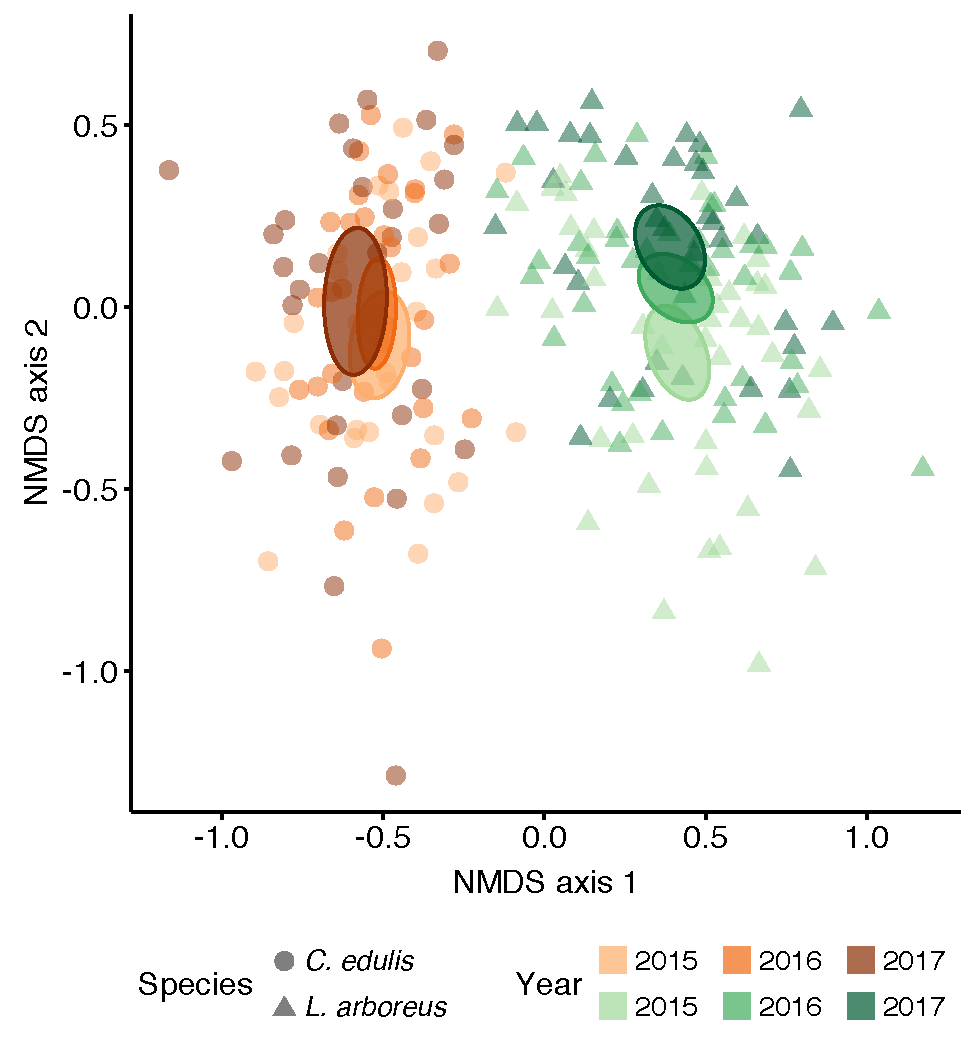
\includegraphics[width=11cm]{Chapter5/3YrNMDS_Species_Common.pdf}}
	\caption[Compositional differences among fungal communities associated with plant individuals across three sampling years.]
		{\hspace{1mm} Compositional differences among fungal communities associated with plant individuals across three sampling years. Each point represents the fungal community of one plant individual. Point shapes represent plant species (circle: \textit{C. edulis}; triangle: \textit{L. arboreus}) and the brightness of colors represent the year of sampling (light orange/green: 2015; orange/green: 2016; dark orange/green: 2017). Ellipses represent the standard error of all points that were collected from the same species during the same year. 
		% See Fig.~\ref{fig:3YrNMDS_Sample} for identical pattern when soil samples, instead of plant individuals, were plotted as observation units.
		}
	\label{fig:3YrNMDS_Individual}
\end{figure}



\clearpage
\begin{figure}[h]
	\centering
	\makebox[\textwidth][c]{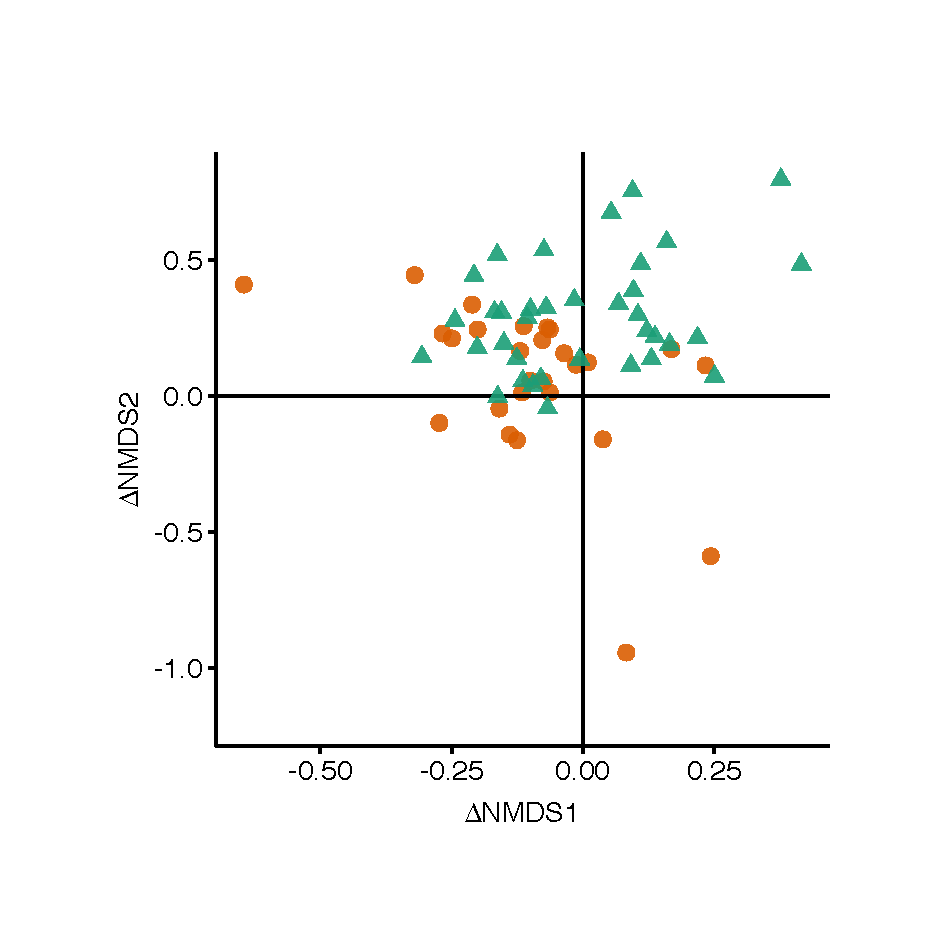
\includegraphics[width=12cm]{Chapter5/FourQuadrateMovement_Species_Common_RevisedMS.pdf}}
	\caption[Overall compositional shifts of the fungal community from 2015 to 2017.]
		{\hspace{1mm} Overall compositional shifts of the fungal community from 2015 to 2017. Each point represent the movement (i.e., x- and y-component of the arrow) of the fungal community associated with one plant individual. A positive x-component (i.e., $\Delta$NMDS 1 $ > 0$) and y-component (i.e., $\Delta$NMDS 2 $ > 0$) represents a rightward and upward movement, respectively. Point shapes and colors represent plant species (orange circle: \textit{C. edulis}; green triangle: \textit{L. arboreus}). See also Fig.~\ref{fig:FourQuadrate_Individual_Species_SI} for movement among consecutive sampling years.
		% See Fig.~\ref{fig:FourQuadrate_Sample_Species} for identical pattern when soil samples were plotted as observation units.
		}
	\label{fig:FourQuadrate_Individual_Species}
\end{figure}



\clearpage
\begin{figure}[h]
	\centering
	\makebox[\textwidth][c]{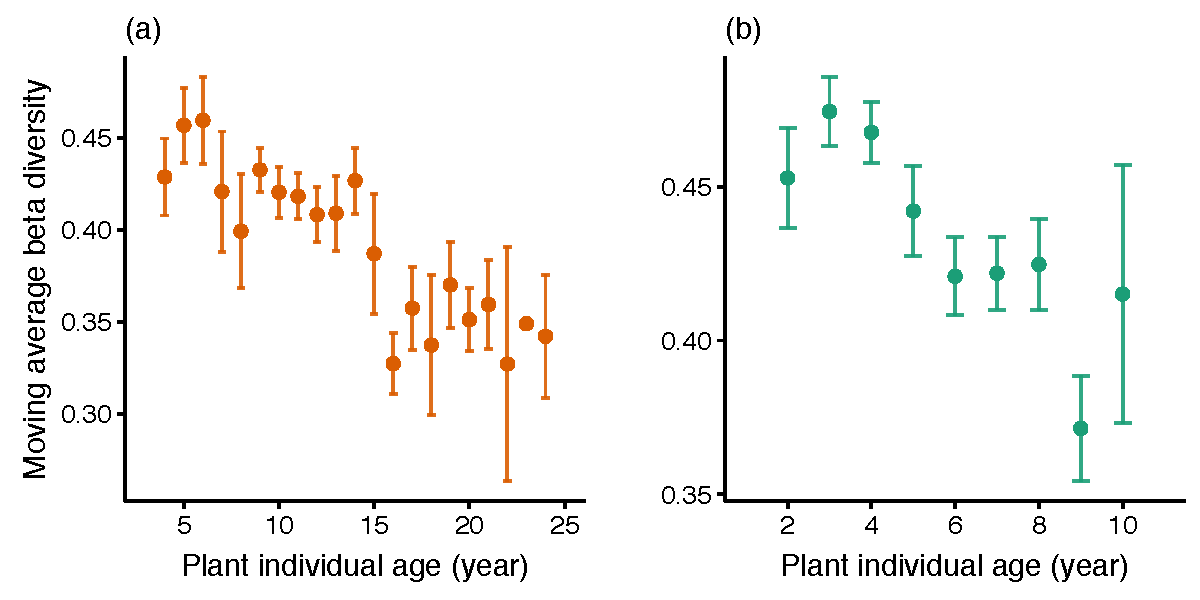
\includegraphics[width=15cm]{Chapter5/BetaDiversity_CompiledFull2015_Common_RevisedMS.pdf}}
	\caption[The relationship between plant age and beta diversity of fungal communities associated with chronosequence plant individuals when a three-year moving window was applied.]
		{\hspace{1mm} The relationship between plant age and beta diversity of fungal communities associated with chronosequence plant individuals.
		(a) and (b) show the pattern for microbial communities associated with \textit{C. edulis} (orange) and \textit{L. arboreus} (green), respectively.
		Points and error bars show the moving average trend (mean $\pm$ SE) when a three-year moving window was applied (i.e., the centroid was calculated using fungal communities associated with individuals of age $\tau - 1$, $\tau$, and $\tau + 1$; see main text for details). 
		Figure~\ref{fig:CombinedFull2015Beta_Individual_SI} shows similar trends when beta diversity was calculated as the distance of fungal communities to their age-specific centroid. 
		% See Fig.~\ref{fig:Full2015Beta_Sample} for the pattern when soil samples were plotted as observation units.
		} 
	\label{fig:CombinedFull2015Beta_Individual}
\end{figure}



\clearpage
\begin{figure}[h]
	\centering
	\makebox[\textwidth][c]{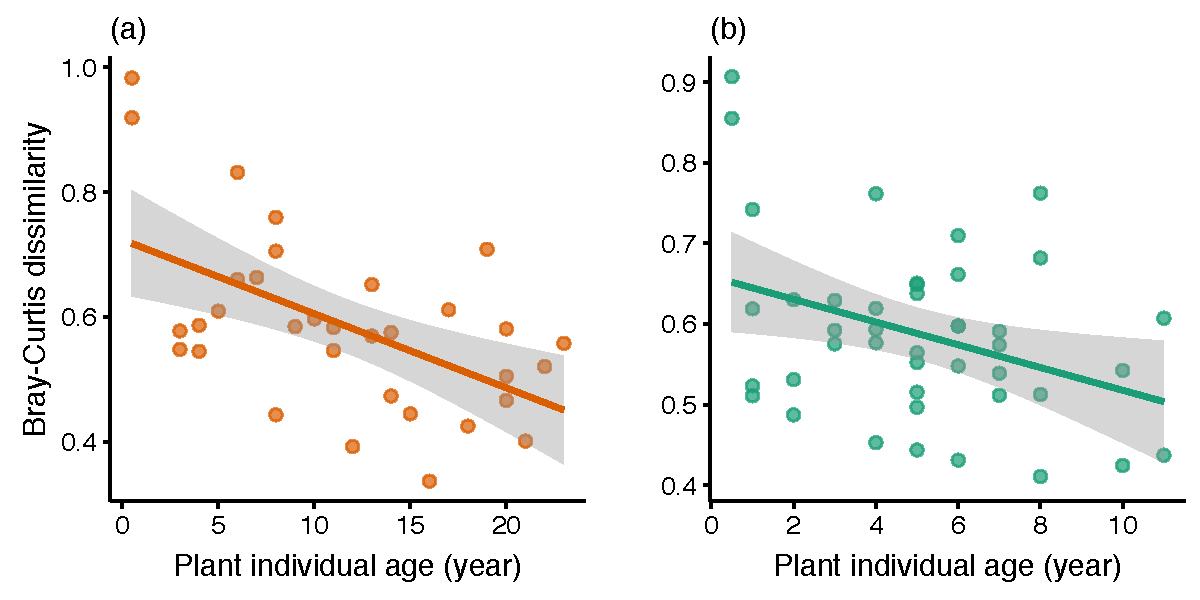
\includegraphics[width=15cm]{Chapter5/Goodness_FungiSpecies_CombinedIndividual_Full2015glmmTMBTotal_Revised2MS.pdf}}
		\caption[The relationship between plant age and Bray--Curtis dissimilarity between the fungal community observed in 2016 and the 2015 chronosequence prediction.]
		{\hspace{1mm} The relationship between plant age and Bray--Curtis dissimilarity between the fungal community observed in 2016 and the 2015 chronosequence prediction.
		(a) and (b) show the pattern for microbial communities associated with \textit{C. edulis} (orange) and \textit{L. arboreus} (green), respectively. 
		Each point represents the dissimilarity calculated for a fungal community, using samples collected in 2016 as the validation test set. See also Fig.~\ref{fig:HMSC_Species_Individual_Full2015_SI} for similar patterns when samples collected in 2017 were used as the validation test set.
		% See Fig.~\ref{fig:HMSC_Species_Sample_Full2015} or identical pattern when soil samples were plotted as observation units.
		}
	\label{fig:HMSC_Species_Individual_Full2015}
\end{figure}



\clearpage
\begin{figure}[h]
	\vspace*{-1cm}
	\centering
	\makebox[\textwidth][c]{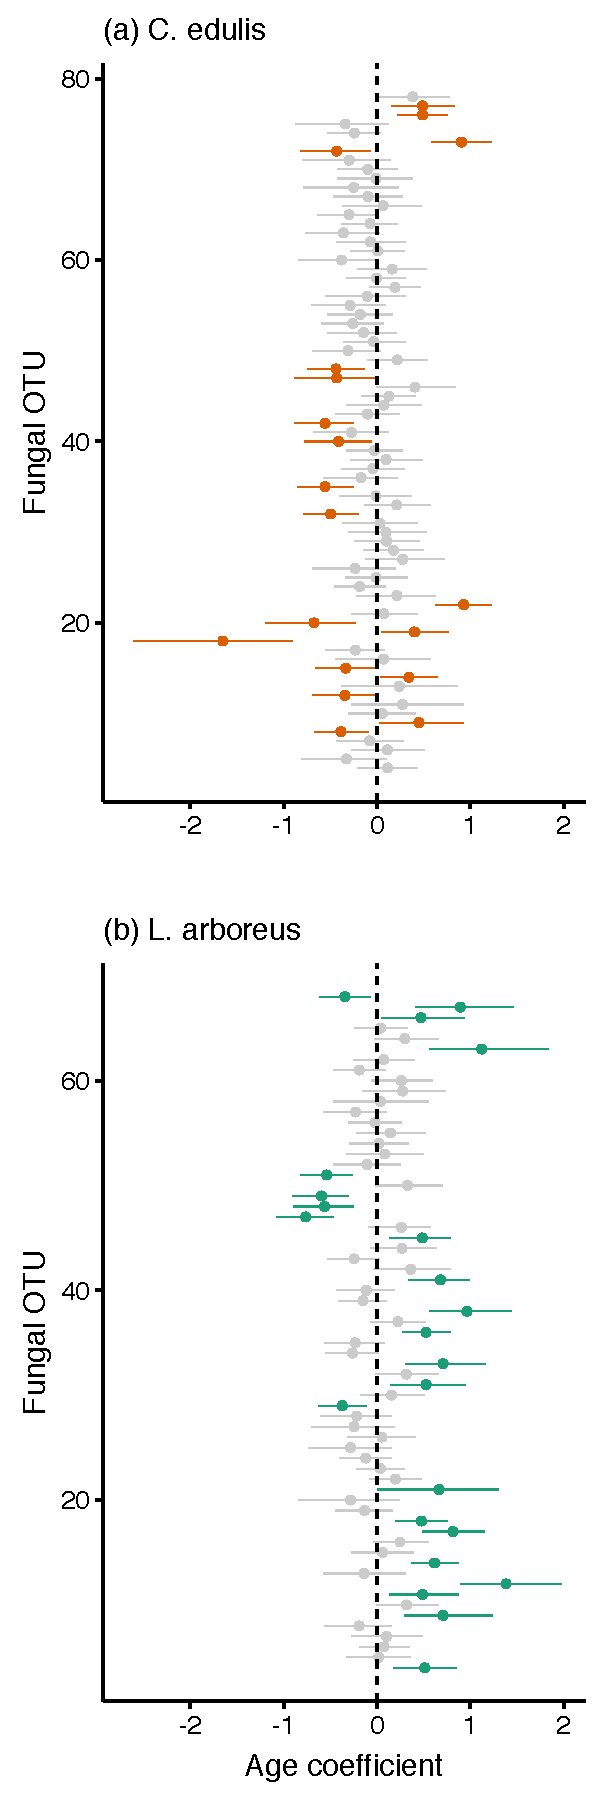
\includegraphics[width=6.5cm]{Chapter5/Funguild_HMSC_FungiSpecies_CombinedIndividual_Full2015Total_PathogenLong.pdf}}
	\caption[Predicted temporal trends of potential pathotrophic fungal OTUs associated with \textit{C. edulis} and \textit{L. arboreus} individuals.]
		{\hspace{1mm} Predicted temporal trends of potential pathotrophic fungal OTUs associated with (a) \textit{C. edulis} and (b) \textit{L. arboreus} individuals. Model fitting was performed for the two plant species separately. Points and line segments represent the mean and the 95$\%$ credible interval of the fitted age coefficient (x-axis) for different fungal OTUs (y-axis). Significant age coefficients are colored (orange for \textit{C. edulis}; green for \textit{L. arboreus}) and insignificant ones are in gray.}
		\label{fig:Funguild_HMSC_Species_Individual_Full2015Pathogen}
\end{figure}



\chapter{Dynamic plant--soil microbe interactions: the neglected effect of soil conditioning time}
%\chaptermark{Positive frequency-dependence}
%\renewcommand{\sectionmark}[1]{}
\fancyhead[LE, RO]{\thepage}
\fancyhead[RE]{CHAPTER 6}
\fancyhead[LO]{TEMPORAL PLANT--SOIL FEEDBACK}
\fancyfoot{}
\renewcommand{\headrulewidth}{0pt}
\setlength{\parindent}{1cm}



\begin{comment}
\documentclass[hidelinks,letterpaper, 11pt]{article}
\usepackage{graphicx, bm, booktabs, lineno, array}
\usepackage[fleqn]{amsmath}
\usepackage{nicefrac}
\usepackage[compress,comma]{natbib}
\usepackage[right=1in, left=1in, top=1in, bottom=1in]{geometry}
\usepackage[parfill]{parskip}
\usepackage[usenames,dvipsnames]{color}
\usepackage[font=large,labelfont=bf,margin=1cm, labelsep = none]{caption} % caption formatting
\usepackage{setspace}
\usepackage{gensymb}
\usepackage{color}
\usepackage{sidecap}
%\usepackage{floatrow}
\usepackage{etoolbox}
\usepackage{tcolorbox}
\usepackage{newpxtext,newpxmath}
\tcbuselibrary{breakable}
%\usepackage{indentfirst}
\newbool{MyRefNumbers}
\usepackage{authblk}
\usepackage{hyperref}
\usepackage{mathpazo}
\usepackage[color=cyan, textsize=tiny]{todonotes}
\usepackage[font={normalsize}]{caption}
\usepackage{adjustbox}
\usepackage{array}
\usepackage{booktabs}
\usepackage{multirow}
\usepackage{tabularx}
% \usepackage{titling}

\setlength{\mathindent}{0pt}
\setlength{\parindent}{1cm}
% \makeatletter
% \makeatother
\pdfminorversion=3

% For table
\newenvironment{myindentpar}[1]%
{\begin{list}{}%
		{\setlength{\leftmargin}{#1}}%
		\item[]%
	}
	{\end{list}}
\newcommand*\samethanks[1][\value{footnote}]{\footnotemark[#1]}
\newcommand\blfootnote[1]{%
	\begingroup
	\renewcommand\thefootnote{}\footnote{#1}%
	\addtocounter{footnote}{-1}%
	\endgroup
}
\newcommand{\plus}{\raisebox{.4\height}{\scalebox{.6}{+}}}
\newcommand{\minus}{\raisebox{.4\height}{\scalebox{.8}{-}}}
% Command to recount supplement
\newcommand{\beginsupplement}{%
	\setcounter{table}{0}
	\renewcommand{\thetable}{S\arabic{table}}%
	\setcounter{figure}{0}
	\renewcommand{\thefigure}{S\arabic{figure}}%
}
% Command to center oversized images in floats
\newcommand{\centerfloat}{%
	\parindent \z@
	\leftskip \z@ \@plus 1fil \@minus \textwidth
	\rightskip\leftskip
	\parfillskip \z@skip}
\renewcommand\Affilfont{\fontsize{12}{12}\selectfont}
\newcommand{\ignore}[2]{\hspace{0in}#2}
\end{comment}



\begin{comment}
\begin{document}

\doublespacing
\title{Dynamic plant--soil microbe interactions: \\ the neglected effect of soil conditioning time}
\author[1, $\dagger$]{Po-Ju Ke}
\author[2]{Peter C. Zee}
\author[1, $\dagger$]{Tadashi Fukami}
\affil[1]{Department of Biology, Stanford University, Stanford, California, 94305, USA}
\affil[2]{Department of Biology, University of Mississippi, University, Mississippi, 38677, USA}
\date{\today}
\maketitle
\blfootnote{$\dagger$ Correspondence author: Department of Biology, Stanford University, Stanford, California 94305-5020, USA. Phone: +1 650-721-1711. Fax: +1 650-723-6132. Email: pojuke@stanford.edu, fukamit@stanford.edu}
	
\onehalfspacing
\noindent \textbf{Running title:} Temporal development of plant--soil feedback\\
\noindent \textbf{Keywords:} aerial photos, chronosequence, microbial community, plant--soil feedback, sand dunes, space-for-time substitution\\
\noindent \textbf{Type of article:} Letter\\
	
\begin{myindentpar}{1cm}
	\textbf{Words in Abstract:} 150\\
	\textbf{Words in main text:} $\sim$ 4000\\
	\textbf{Number of references:} 63\\
	\textbf{Number of figures:} 5\\
\end{myindentpar}
	
\noindent \textbf{Authorship statement:} PJK and TF conceived the study; PJK conducted the study and analyzed the data; PJK and PCZ developed the model and performed the simulation; PJK wrote the first draft of the manuscript with substantial contribution from all authors.\\
	
\noindent \textbf{Data accessibility statement:} Should the manuscript be accepted, all data and computer scripts supporting the results will be archived in a public Github repository, with the DOI included at the end of the article.\\

\linenumbers
\doublespacing
\end{comment}



\section{Abstract}
Plant--soil feedbacks (PSF), the reciprocal interactions between plants and soil microbes, shape the structure of plant communities, but how the length of soil conditioning affects PSF strength is rarely studied. 
Using a chronosequence reconstructed from aerial photos, we characterized the soil microbial communities associated with four perennial dune plants and their turnover as plants aged. 
We also quantified PSF strength in a greenhouse experiment that preserved age-specific soil properties.
For all plants, we found that their microbial communities changed with increasing conditioning time.
The greenhouse experiment showed that these compositional turnovers caused PSF strength to change in ways that depended on the specific plant--soil combination. 
With an individual-based simulation model, we further found that the temporal development patterns of PSF affected the rate of plant community convergence. 
Taken together, we suggest that future studies should consider the temporal development pattern of PSF to understand its effects on plant community assembly.
\medskip


\noindent \textbf{Keywords:} aerial photos, chronosequence, microbial community, plant--soil feedback, sand dunes, space-for-time substitution



\section{Introduction}
%Plant-soil interactions are important and assumed to be constant
It is widely recognized that interactions between plants and soil microbes, known as plant--soil feedbacks (PSF), can affect the structure of plant communities \citep{Bever2010, vanderPutten2013, KeMiki2015}. 
Plants cause changes in the composition of the soil microbial community, which then feeds back to affect the growth of neighboring plants \citep{Bever1997, Bever2003}. As plant species vary in their response to soil microbes, PSF can modify differences in plant performance and alter plant community composition \citep{Klironomos2002, Mangan2010, Eppinga2018}.
The strengths of these feedbacks are commonly assumed to be constant through time \citep{Kardol2013}. Under this assumption, most empirical studies quantify feedback strengths via short-term greenhouse experiments that are terminated at the same time for all species \citep{KulmatiskiKardol2008, Kardol2013}. The estimated feedback strengths are then incorporated into theoretical models as time-independent parameters (e.g., \citealp{Fukami2013, Bauer2015, Teste2017}). 
\par


%The importance of a dynamic PSF viewpoint
Recent studies have started to recognize that PSF strength can vary across plant life stages due to ontogenetic changes in plant's responses to soil microbes \citep{Hawkes2012, Dudenhoffer2017, Bezemer2018}. 
Temporal development of PSFs can also be driven by changes in microbial community composition with plant age (i.e., the duration of soil conditioning), which proceeds at different rates depending on host plant identity \citep{Knelman2012}. 
Explicit consideration of the effects of soil conditioning length, however, is lacking in the current PSF literature probably owing to two logistical challenges. First, preparing soils with different conditioning lengths is often not feasible in the greenhouse \citep{Kardol2013, Kulmatiski2018}, and second, the length of soil conditioning in the field can only be quantified with coarse resolution due to uncertainty about the ages of individual plants (e.g., \citealp{Speek2015, Day2015}).
\par


%Aim of paper
In this paper, we study how PSF strengths vary with the length of soil conditioning and how the temporal patterns differ among plant species. 
To this end, we used high-resolution aerial photos of the coastal dune vegetation at Bodega Bay in California, which were taken annually from 1992 to 2016. This unique resource allowed us to estimate the age of individual plants and use it as a proxy for soil conditioning length. 
By sampling soils from individual plants of different ages, we applied a chronosequence approach to examine how soil microbial communities vary across plant species and conditioning time. We then designed a greenhouse experiment that preserved plant age-specific microbial communities to study how changes in their composition affected species' PSF strength.
This combination of approaches allowed us to overcome the logical challenges outlined above and study the link between plant age, soil microbial composition, and feedback strength. 
Finally, we used a general individual-based simulation model to explore how the temporal pattern of PSF may affect plant community assembly and their transient dynamics.
\par



\section{Methods}
\subsection*{Study system}
%Basic information and natural history of Bodega bay 
We conducted our study at the coastal foredunes of Bodega Bay, California, USA (38$^{\circ}$19$^\prime$ N, 123$^{\circ}$3$^\prime$ W), located within UC Davis Bodega Marine Reserve and Sonoma Coast State Beaches. This region experiences a Mediterranean-type climate, with an average annual temperature of 15.8$^{\circ}$C and annual precipitation of 760 mm, mostly occurring between October to April \citep{Barbour1973, Conser2009}. The soils in our 400 $\times$ 500 m study area are predominantly sand, with a negligible amount of silt and clay \citep{Kleinhesselink2014}. 
We focused on the four dominant species of the foredune plant community, including the introduced grass \textit{Ammophila arenaria} (Poaceae), the introduced succulent dwarf-shrub \textit{Carpobrotus edulis} (Aizoaceae), and the native shrubs \textit{Baccharis pilularis} (Asteraceae) and \textit{Lupinus arboreus} (Fabaceae). 
\par



\subsection*{Soil sampling}
%Plant individual selection
We used a series of aerial photos that were taken annually by Delta Geomatics Corporation, and curated by the Bodega Marine Reserve, from 1992 to 2016 \citep{Danin1998}. Since the foredune vegetation has little vertical structure, we were able to identify plant individuals to the species level and estimate their age (i.e., identify the first year the individual appeared in the photos) by comparing photos across multiple years. Age estimates were used as proxies for soil conditioning length as the foredune undergoes primary succession starting from unconditioned bare sand. 
For each of the four dominant species, we selected 30 individuals of different ages along the chronosequence. All individuals were selected to sample evenly along the plant's age span provided by the aerial photos, which ranged between 1 to 11 years for \textit{L. arboreus} and between 2 to 25 years for the other three species.
No spatial autocorrelation was evident for the age of selected individuals (Moran's I, $P = 0.24$; Mantel test, $P = 0.39$). 
See Fig.~\ref{fig:map} for a representative aerial photo, the spatial distribution of selected individuals, and representative examples of different age classes for each species.
\par


%Soil sampling for microbial community patterns
To study how soil microbial communities varied with plant age, in July 2016 we collected three soil samples beneath each plant individual (i.e., at azimuth angles 0$^{\circ}$, 120$^{\circ}$, and 240$^{\circ}$) in separate sterile 50 mL Falcon tubes. 
An additional 3 and 13 individuals of \textit{C. edulis} and \textit{L. arboreus}, respectively, were sampled for this microbial community survey. We also collected soil samples from three randomly selected juveniles (i.e., one sample per juvenile, which are individuals that germinated within one year and were too small to be visible on the aerial photos from the previous year) for three of the four species (i.e., all but \textit{A. arenaria}). Finally, a total of 13 soil samples from randomly selected bare sand areas (i.e., no vegetation in an approximately 3 m radius throughout the entire length of time of the aerial photos) were collected across our field site (Fig.~\ref{fig:map}). 
All soil samples were stored at 4$^{\circ}$C before being processed in the lab. Within one week after collection, soil samples were processed by passing through a sterile 2 mm mesh sieve and homogenized thoroughly in separate sterile plastic bags.
The fungal and bacterial communities of the resulting 430 soil samples (i.e., 136 individuals $\times$ 3 samples + 3 species $\times$ 3 juveniles + 13 bare sand samples) were characterize with next-generation sequencing (see section `\textit{DNA sequencing of fungal and bacterial communities}').
\par



\subsection*{DNA sequencing of fungal and bacterial communities}
%Brief overview of NGS flow
For each processed soil sample collected in July 2016, we extracted microbial DNA from 0.25 g of subsampled soil with the PowerSoil DNA Isolation Kit. We then PCR-amplified the bacterial 16S ribosomal DNA region and the fungal internal transcribed spacer 1 region (ITS1) with specific primer pairs \citep{Caporaso2012, Toju2012, Lundberg2013, Hamady2008}. Amplicon libraries were then normalized, pooled, sequenced by the Illumina MiSeq sequencer, and processed through a bioinformatic pipeline \citep{Wang2007, Edgar2011, McMurdie2013, Tanabe2013, Zhang2014, Deshpande2016, Rognes2016, Davis2018} to obtain a rarefied sample $\times$ operational taxonomic units (OTUs) matrix. See Appendix E.1 for detailed description.
\par



\subsection*{Greenhouse experiment}
To examine changes in the effects of soil microbial communities on plant performance in a greenhouse experiment, we revisited the same plant individuals in July 2017. 
For all four species, we collected 300 mL of soil from each individual within a random subset of previously sampled individuals ($N = 27$). Soils were collected, and pooled together, from three positions adjacent to the original sampling position in 2016 (100 mL from each position using a sterile soil core sampler). We also collected the same amount of soil from three new randomly selected juveniles for all four species. 
Soils collected from all 120 individuals (i.e., 4 species $\times$ 27 individuals + 4 species $\times$ 3 juveniles) were processed with the same method as above and stored at 4$^{\circ}$C before the greenhouse experiment.
\par


%Soil preparation for the greenhouse experiment
Our greenhouse experiment used soil samples collected in July 2017 and was performed in two separate rounds, which started in late August and September 2017, respectively.
Soils collected from different plant individuals were kept separated throughout the experiment so that each soil maintained its age-specific properties \citep{Rinella2018}.
The range and variance of plant individual age were kept similar among the two experiment rounds (i.e., by sorting individuals based on their age and assigning every other individual along the age axis to different experiment round). 
Half of the soil volume collected from each individual was autoclaved to create a sterile treatment, allowing us to isolate the effects of soil microbial communities. 
Soils collected from 9 individuals were discarded due to handling mistakes (i.e., 6 and 3 individuals for the first and second round, respectively), resulting in a total of 222 unique soil environments that differed in their host plant species, individual age, and sterilization treatment (i.e., 111 individuals $\times$ 2 sterilization treatments).
\par


%Seedling transplant for the greenhouse experiment
Seeds of the four species were surface-sterilized and allowed to germinate on autoclaved sand under controlled condition (see Appendix E.1). After two weeks, we transplanted the seedlings individually into 107 mL ``cone-tainer'' pots (i.e., one seedling per pot) filled with 80 mL of sterilized sand and added 20 mL of either live or sterile soil inoculum to the top. 
Our experiment examined the full combination of transplanting each of the four species into all 222 soil environments. However, \textit{B. pilularis} was omitted during the second round due to low germination rate, resulting in a total of 774 pots (i.e., 432 in the first round (54 individuals $\times$ 2 sterilization treatments $\times$ 4 species) and 342 in the second round (57 individuals $\times$ 2 sterilization treatments $\times$ 3 species); see Appendix E.1 for detail).
Seedlings grew in the greenhouse for 12 weeks, after which we harvested and oven-dried all plant tissues from each pot at 70$^{\circ}$C for 96 h. The resulting total dry biomass was weighed to quantify the effects of soil microbes on plant performance.
\par



\subsection*{Data analysis}
%Distance-based community level analysis for microbial communities
We analyzed the fungal and bacterial communities separately. To better match our microbial community data from soil samples to the soils used in our greenhouse experiment, we summed the OTU reads of the three samples that belonged to the same plant individual. As a result, the following statistical analyses were performed by viewing plant individuals as the unit of replication. 
To examine how alpha diversity of the microbial community varied with plant age, we fitted linear, quadratic, and Monod functions (with R package nlme) to model ln(observed OTU richness) as a function of plant age. Models were fitted for each plant species separately, and the best model was selected based on their AICc values.
To visualize compositional differences among microbial communities, we used non-metric multidimensional scaling (NMDS) to ordinate microbial communities based on Bray-Curtis dissimilarity matrices (with R packages vegan and phyloseq). Effects of soil host species identity and plant age on microbial community composition were tested with permutational multivariate analysis of variance (PERMANOVA with 999 permutations, \citealp{Anderson2011}). 
To identify the microbial taxonomic groups that drove the observed community pattern, we aggregated the microbial communities to the family level and modeled the abundance of each family as a function of plant age using the R package HMSC (\citealp{Ovaskainen2017}, see Appendix E.1 for detail). 
Note that all statistics with plant age as a predictor were performed for each plant species separately. This is because species vary in their longevity and thus the same age does not necessarily represent the same life stage for different species.
\par


%Defining our PSF index
In our greenhouse experiment, seedlings of the same plant species were paired based on the plant individual where field soils were collected, with one seedling inoculated with live soil and the other with sterile soil from the same plant individual. As soils from different individuals were not mixed \citep{Rinella2018}, we were able to quantify the effects that the soil microbial community from a $k$-year-old individual of species $j$ (denoted as the $j^{k}$ individual) had on species $i$ as:

\begin{equation}
\sigma_{i, \,j^{k}} = \textup{log}_{10}(\frac{B_{i, \,j^{k}, \,live}}{B_{i, \,j^{k}, \,sterile}}), \nonumber
\end{equation}

\noindent where $B_{i, \,j^{k}, \,live}$ and $B_{i, \,j^{k}, \,sterile}$ represent seedling biomass of species $i$ when grown in soils inoculated with either live or sterile soil from the $k$-year-old individual of species $j$, respectively. Since the inocula used in the two biomass measurements were collected from the same plant individual in the field, the resulting metric is an ``age-specific microbial effect'' associated with the $j^{k}$ individual. A positive (or negative) value means that the soil microbial community associated with the $j^{k}$ individual had a net beneficial (or detrimental) effect on the seedling of species $i$. For this paired calculation, data for 20 live--sterile soil pairs were discarded due to seedling death or handling mistakes. 
\par


%Statistical tests with the PSF index  -- static perspective
We used two approaches to analyze the age-specific microbial effects. First, we took the time-averaged value of $\sigma_{i, \,j^{k}}$ for each plant $\times$ soil host species combination (i.e., ignored the age information by taking the temporal mean), which is the common approach used in studies when the information of soil conditioning length is not available. 
For each of the four plant species, the effects of soil host species on the time-averaged microbial effect were tested by fitting generalized linear mixed models (GLMM, with normal distribution of errors using R package lme4). We included the identity of soil host species as a fixed effect and greenhouse round, when present, as a random effect. Post-hoc group comparisons with Holm--Bonferroni adjusted probabilities were performed (with R package multcomp).
For each of the 16 plant $\times$ soil host species combinations, an additional \textit{t}-test was used to test if the time-averaged microbial effect was significantly different from zero.
\par
 
 
%Statistical tests with the PSF index  -- dynamics perspective
The second approach took advantage of the age information provided by the aerial photos. Specifically, we visualized the age-specific microbial effects on the temporal axis (i.e., soil conditioning length) and quantified the temporal development pattern for each of the 16 plant $\times$ soil host species combinations.
We applied a two-step process to test if the strength of microbial effects varied with increasing conditioning time. First, we fitted separate GLMMs with plant age as a fixed effect and greenhouse round as a random effect for each of the 16 plant $\times$ soil host species combinations. For this step, we fitted both linear and quadratic functional forms and selected the best model based on their AICc values. 
Second, for temporal patterns that were not statistically significant, we fitted a Monod function to assess how fast the microbial effects would build up. If both steps of the fitting procedure resulted in a poor model fit (i.e., age had no significant effects, and the nonlinear Monod fitting procedure failed to converge), we concluded that the length of soil conditioning had little influence on the microbial effect for this plant $\times$ soil host species combination. All analyses and simulations were performed in \textit{R} version 3.3.1 \citep{R}. 
\par



\subsection*{Simulation model}
To further study how the temporal development of PSF affects plant community assembly, we constructed a general individual-based model following \citet{FukamiNakajima2011} (see also \citealp{Fukami2013, ZeeFukami2015, Fukami2017}). 
% We constructed a general individual-based model following \citet{FukamiNakajima2011} (see also \citealp{Fukami2013, ZeeFukami2015, Fukami2017}). 
Our simulation exercise focuses on both transient and steady states of plant community assembly and explores the potential consequences of different temporal development patterns of PSF.
The model consists of species pools containing 50 species (each with a different trait value) and patches consisting of 1024 local sites (each with a different habitat conditions). We simulated the processes of immigration, reproduction, arrival, competition for establishment, and death of plant individuals. 
Competition for establishment at empty sites is determined not only by the match between species' trait values and local habitat conditions (i.e., environmental filtering) but also by the soil microbial legacy effects (i.e., PSF) created by the previously established plant species. 
Based on empirical evidence, we allowed the microbial legacy effects to be either positive or negative (i.e., complex feedback regime, \textit{sensu} \citealp{Fukami2013}).
The key distinction between our model and previous studies is that microbial legacy effects in our model are age-dependent, i.e., the strength depends on the age of death of the previous established individual. See Appendix E.1 for full details of the simulation model.
\par


For our simulation, we generated 10 patches for the regional species pool to colonize independently and one set of baseline microbial legacy effects, which represent the microbial effects created by the previous individual if it died a year immediately after colonization.
The microbial effects experienced by a new arriving species depends on the previous individual's age of death and the temporal development pattern of microbial effects.
Here, we considered four scenarios: (1) `constant', where microbial effects remain unchanged despite individuals becoming older; (2) `magnifying', where both positive and negative microbial effects intensify in strength as individuals become older (i.e., the longer the previous individual lived before it died, the stronger its impact on the new individual); (3) `decaying', where both positive and negative microbial effects attenuate in strength as individuals become older; and (4) `bidirectionally varying', where both intensifying and attenuating are possible. 
For each scenario, we simulated 20 replicated runs of community assembly, where 20 independently created sets of species pool (each with 50 species) were allowed to colonize the same set of 10 patches, using the same set of baseline microbial effects. 
We quantified the beta diversity among the 10 patches for each replicated run, which is measured as the gamma diversity divided by the mean alpha diversity, and compared the temporal patterns of beta diversity among different scenarios.
\par



\begin{comment}
% PBA-1: This comes out of the blue a little. Needs better motivation. (DONE: changed the motivation sentence)
% PBA-2: I was also left wondering why you don't seem to use your field data to inform this model, shouldn't the temporal patterns of PSF development match your field results? (CANNOT DO) 
% PBA-3: And why is community convergence the key response? Rather than something like richness or abundance distribution? (CONE: it's actually the only meaningful comparison in this model, downplayed it term) 
% EGM-1: Why didn’t you simply parameterize the model using the empirical PSF measurements for your 4 species, and simulate the dynamics through time? Some justification of this approach is needed. (CANNOT DO)
% EGM-2: Again, justify this decision because it seems very arbitrary. Why not use all 50 species in the community assembly simulation, for example? (CAN DO: clarify this specific question about the generation of replicated species pool)
\end{comment}


% We simulated 20 replicated runs of community assembly, where 20 independently created sets of species pool (each with 50 species) were allowed to colonize the same set of 10 patches, using the same set of microbial legacy effects. Following our empirical results, we allowed the microbial legacy effects to be either positive or negative (i.e., complex feedback regime, \textit{sensu} \citealp{Fukami2013}). For all microbial effects created by the previously established individual, four temporal development scenarios were considered: (1) `constant', where microbial effects remain unchanged despite individuals becoming older; (2) `magnifying', where both positive and negative microbial effects intensify in strength as individuals become older (i.e., the longer the previous individual lived before it died, the stronger its impact on the new individual); (3) `decaying', where both positive and negative microbial effects attenuate in strength as individuals become older; and (4) `bidirectionally varying', where both intensifying and attenuating are possible. For each scenario, we quantified the beta diversity among the 10 patches for replicated run, which is measured as the gamma diversity divided by the mean alpha diversity, and compared the temporal patterns of beta diversity (i.e., detecting community convergence or divergence) among different scenarios.



\section{Results}
\subsection*{Temporal patterns of microbial communities}
Fungal community composition differed among plant species (Fig.~\ref{fig:BothComposition}a, PERMANOVA, $R^{2}=0.148$, $P<0.001$). Within each plant species, fungal composition varied with plant age (Fig.~\ref{fig:FunComposition}, age effect for \textit{A. arenaria}: $R^{2}=0.096$; \textit{B. pilularis}: $R^{2}=0.083$; \textit{C. edulis}: $R^{2}=0.100$; \textit{L. arboreus}: $R^{2}=0.077$; all $P<0.001$) and became progressively different from bare sand communities with increasing conditioning time (fungal richness ceased to increase further after a few years following plant colonization, Fig.~\ref{fig:FunRichness}).
Similar results were observed for bacterial communities (Figs.~\ref{fig:BothComposition}b, \ref{fig:BacRichness}, and \ref{fig:BacComposition}, species effect: $R^{2}=0.126$; age effect for \textit{A. arenaria}: $R^{2}=0.115$; \textit{B. pilularis}: $R^{2}=0.112$; \textit{C. edulis}: $R^{2}=0.120$; \textit{L. arboreus}: $R^{2}=0.116$; all $P<0.001$). 
Fungal and bacterial families responded differently to increasing plant age, and the temporal changes of a family depended on the identity of the plant species (Figs.~\ref{fig:FunHMSC} and \ref{fig:BacHMSC}). 
\par



\subsection*{Temporal patterns of soil microbial effects on plant performance}
%Time-averaged PSF index -- static perspective
By quantifying the time-averaged microbial effects that each plant species experienced when grown in soils conditioned by different soil host species, we found that the effects of soil microbes were largely determined by the seedling's species identity.
In particular, the microbial effects was positive for \textit{L. arboreus} but negative for the other three species (Fig.~\ref{fig:PSFBar}). 
Most microbial effects were significantly different from zero ($P<0.05$; expect for \textit{B. pilularis} when grown in soils from \textit{A. arenaria} and \textit{L. arboreus} individuals; Fig.~\ref{fig:PSFBar}b), but the identity of the soil host species had little effect on the microbial effects that plants experienced (soil host species effect for \textit{A. arenaria}: $F_{3, 103.05}=0.39$, $P=0.76$; \textit{B. pilularis}: $F_{3, 45}=0.27$, $P=0.27$; \textit{C. edulis}: $F_{3, 97.18}=2.07$, $P=0.11$; Fig.~\ref{fig:PSFBar}a--c). The only exception was \textit{L. arboreus}, which grew best in soils from \textit{C. edulis} individuals and worst in soils from \textit{A. arenaria} individuals (soil host species effect: $F_{3, 103.07}=3.55$, $P=0.02$; Fig.~\ref{fig:PSFBar}d).
\par


%Temporal development of PSF index -- dynamic perspective
Despite little effect of the soil host species identity on the time-averaged microbial effects, the temporal development pattern of the microbial effects depended on the plant $\times$ soil host species combination (Fig.~\ref{fig:PSFTemporal}). 
For example, \textit{A. arenaria} and \textit{C. edulis} experienced stronger negative microbial effects when grown in conspecific soils with a longer conditioning history (Fig.~\ref{fig:PSFTemporal}a and k). However, temporal patterns were different when these two introduced species grown in heterospecific soils conditioned by each other: the negative microbial effects that \textit{A. arenaria} imposed on \textit{C. edulis} intensified through time (Fig.~\ref{fig:PSFTemporal}i), whereas no significant temporal pattern was detected for the opposite pair (Fig.~\ref{fig:PSFTemporal}c).
The positive microbial effects that \textit{L. arboreus} experienced were instantaneous (Fig.~\ref{fig:PSFTemporal}m--o), and the microbial effects that \textit{L. arboreus} imposed on conspecies and \textit{C. edulis} did not show statistically significant temporal patterns (Fig.~\ref{fig:PSFTemporal}l and p).
\par



\subsection*{Effects of temporally varying soil microbial effects on plant community assembly}
%Simulation results
Simulation results showed that plant communities converged in all scenarios, i.e., beta diversity declined through time, as communities became dominated by a subset of species. Despite eventually reaching similar beta diversity value, simulations ran under different temporal development scenarios converged with different rates (Fig.~\ref{fig:SimulationComplexPSF}a). Similar to a previous study \citep{Fukami2013}, beta diversity declined most rapidly when plants did not create microbial legacies (Fig.~\ref{fig:SimulationComplexPSF}b; light gray line in Fig.~\ref{fig:SimulationComplexPSF}a), but was maintained at high levels and declined at slower rates if plants created microbial legacies that maintained a constant strength as individuals became older (Fig.~\ref{fig:SimulationComplexPSF}c; black line in Fig.~\ref{fig:SimulationComplexPSF}a).
When the strength of microbial legacies varied depending on the age of death of the previously established individual, communities converged most rapidly in the decaying scenario (Fig.~\ref{fig:SimulationComplexPSF}e; blue line in Fig.~\ref{fig:SimulationComplexPSF}a), followed by the magnifying scenario (Fig.~\ref{fig:SimulationComplexPSF}c; orange line in Fig.~\ref{fig:SimulationComplexPSF}a), and slowest in the bidirectionally varying scenario (Fig.~\ref{fig:SimulationComplexPSF}f; green line in Fig.~\ref{fig:SimulationComplexPSF}a).
\par



\section{Discussion}
% Result summary and significance statement
By combining a fine-scale chronosequence and a greenhouse experiment that preserved age-specific soil microbial communities, we provide evidence for a temporally varying PSF. 
We show that compositional changes in the soil microbial community with increasing plant age result in different temporal development patterns of PSFs (Figs.~\ref{fig:FunComposition} and \ref{fig:PSFTemporal}), which could in turn influence plant community dynamics (Fig.~\ref{fig:SimulationComplexPSF}). 
\par


We found that microbial richness reached its maximum within a few years after plant establishment (Figs.~\ref{fig:FunRichness} and \ref{fig:BacRichness}), but community composition continued to turn over and became progressively more different from that in bare sand in a manner specific to plant species (Figs.~\ref{fig:FunComposition} and \ref{fig:BacComposition}). 
For example, compared to the other three plant species, soils collected from young \textit{A. arenaria} individuals had microbial communities that were more similar to sand microbial communities, potentially because of their ability to capture more wind-blown sand.
With the model-based approach, we identified potential taxonomic groups that drove the observed turnover in soil microbial communities (Figs.~\ref{fig:FunHMSC} and \ref{fig:BacHMSC}). For instance, the fungal family \textit{Sporormiaceae}, many members of which are saprotrophic fungi, increased through time in soils of the two natives but decreased in \textit{C. edulis} soils presumably because of the recalcitrant litter it produces \citep{Novoa2014}.
Whether turnover of the soil microbial community resulted in temporally varying PSF, however, depended on the plant $\times$ soil host species combination. For example, the microbial community associated with \textit{C. edulis} changed through time (Fig.~\ref{fig:FunComposition}c), but only their effect on conspecifics showed significant temporal patterns (i.e., compare Fig.~\ref{fig:PSFTemporal}k to Fig.~\ref{fig:PSFTemporal}c, g, and o).
Since plant $\times$ soil host species combinations differed in their PSF temporal patterns, the length of soil conditioning set in greenhouse experiments can influence the relative magnitude of species' PSF.
Moreover, by only looking at the time-averaged microbial effects (e.g., if studies homogenized soils collected from individuals of different ages; Fig.~\ref{fig:PSFBar}), one would have erroneously concluded that soil host identity had little impact on the microbial effects that a species experienced in our system.
\par


% Biotic and abiotic mechanisms of the temporally varying PSF
According to the theory of PSF \citep{Bever1997}, a species' feedback strength may vary through time for three non-mutually exclusive reasons: (1) changes in the total density of the species' microbial community compared to that of other plants, (2) changes in the functional composition of the microbial community (e.g., accumulating more pathogenic taxa), and (3) evolutionary changes in the effects of soil microbes on plants (e.g., evolved to become more pathogenic, \citealp{Dostal2013, Packer2004}). The latter two mechanisms would cause the average per-capita effects of soil microbes to vary through time.
Our metric isolates temporal changes in the effect of soil microbes, but soil abiotic properties may also vary with increasing conditioning time and are responsible for changes in plant performance (e.g., \citealp{Lepinay2018}). For example, \textit{C. edulis} produces thick layers of recalcitrant litter through time, which increases organic content but lowers soil pH and harms native species \citep{Conser2009, Novoa2014}. 
\par



\subsection*{Dynamic plant--soil microbe interactions}
% Temporal development during the response phase
Studies aimed at revealing the temporal development of PSF have mostly focused on changes during the response phase, monitoring feedback strengths as plants mature from seedlings to adults \citep{Hawkes2012, Dudenhoffer2017, Bezemer2018}.
For example, \citet{Hawkes2012} conducted a 19-month long experiment and quantified PSF at four different time steps as the planted seedling grew. Their result suggested that PSF strength for native plants became more negative through time. Similar results were also reported in \citet{Dudenhoffer2017}, and these changes could be altered by competitors \citep{Bezemer2018}.
Potential mechanisms for these observed patterns include changes in plant's response to soil microbes across different life stages \citep{Reinhart2010b, Ke2015} and the continuous turnover in soil microbial composition driven by the transplanted seedling as they mature \citep{Husband2002, Meaden2016, Dinnage2019}. 
However, it is difficult to disentangle the underlying mechanisms when experiment were designed to focus only on the response phase. Studies focusing on the temporal development of PSF during the conditioning phase, like our greenhouse experiment, provide the opportunity to isolate the effects of microbial turnover without being confounded by changes in plant responses to soil microbes. 
\par


% Temporal development during the conditioning phase and resident time of invaders
The relationship between soil conditioning length and feedback strength has been investigated in the context of the resident time of invasive plants.
Studies have quantified how the PSF strength experienced by the invading species changes after multiple generations, focusing on how the benefit of escaping host-specific soil pathogens in their native range attenuates with their resident time \citep{Diez2010, Dostal2013, Day2015, Speek2015}. 
For example, \citet{Diez2010} found that non-native plant species that became established in New Zealand for a longer time (e.g., hundreds of years) experienced stronger negative PSF (but see \citealp{Day2015, Speek2015}). 
Here, we provide evidence for how these long-term changes in negative PSF build up within a single generation.
The observed negative PSFs are in line with studies in other similar introduced habitats \citep{delaPena2010, Beckstead2003} and may indicate a decreasing degree of enemy release through time.
\par


% Temporal development during the conditioning phase and  successive planting
% The framework for dynamic PSF
The importance of soil conditioning length has also been highlighted by studies on successive planting. Past studies in agricultural systems found that the performance of crops deteriorates after repeatedly growing the same species in the same field \citep{Mazzola1999, Packer2004}.
% Another line of research related to the soil conditioning length of plants involves successive planting, i.e., repeatedly growing the same species, in agricultural systems \citep{Mazzola1999, Packer2004}. Past studies found that the detrimental effects of soil microbes intensified with increasing rounds of planting, as indicated by increased mortality and decreased biomass in apple \citep{Mazzola1999} and black cherry \citet{Packer2004}.
Recent studies have generalized the traditional focus of single species to consider multiple rounds of soil conditioning by different plant species and in different order \citep{Mariotte2018, Wubs2017, Bezemer2018}.
To synthesize, we suggest that three temporal aspects should be considered: (1) the order of plant species involved in sequential soil conditioning, (2) the length of each conditioning phase and the rate at which soil properties change, and (3) the focal plant individual's life stage and changes in plant responses to soil microbes through their ontogeny. 
\par



\subsection*{Implications for plant community dynamics}
% Implications for priority effect timing and transient dynamics
Our simulation results suggested that, despite eventual convergence, plant communities assembled under different temporal development patterns of PSF would exhibit various transient dynamics and converge at different rates (Fig.~\ref{fig:SimulationComplexPSF}, see also Fig.~\ref{fig:SimulationAllPSF} for other PSF settings).  
Without PSF, species' competitiveness in our simulation model solely depends on environmental filtering (i.e., the match between species' trait value and local habitat condition). All else being equal, communities will be dominated by species with trait values that are closer to the most abundant habitat condition. However, species' competitiveness is modified when plants create PSF, and a more heterogeneous PSF scenario can delay community convergence by preventing the immediate dominance of the species with the best fit trait. 
As a result, communities would converge faster if species' PSF strength became more similar with increasing soil conditioning (e.g., the decaying scenario in Fig.~\ref{fig:SimulationComplexPSF} where microbial legacy effects weakened through time as matured individuals support less pathogens and relied less on mutualists, \citealp{Reinhart2010b}).
\par


% Implications for disturbance, succession, and restoration
Recognizing that PSF is a dynamic process can be useful when studying the effects of PSF on community recovery after disturbance. 
Some disturbance, such as severe wildfire, kills all individuals, whereas other forms of disturbances cause higher mortality for specific age classes \citep{Sousa1984}. For example, insect herbivore outbreak may cause juveniles to suffer higher mortality, whereas windthrow may have a more significant direct impact on large adults \citep{Sousa1984}. These types of disturbances thus terminate soil conditioning at various stages, leaving behind different microbial legacies that could alter recovery trajectories. 
Other studies have also shown that PSF affects restoration \citep{Wubs2016} and exotic plant invasion \citep{Suding2013}. Information on how PSF changes through time can help design restoration projects.
At our field site, we found that \textit{A. arenaria} and \textit{C. edulis} performed worse in conspecific soils with longer conditioning history (Fig.~\ref{fig:PSFTemporal}a and k). 
This result suggests that removing old individuals may be an effective restoration strategy since the microbial legacies that they leave behind are detrimental for propagules from nearby non-native individuals to regenerate. 
\par



\section{Conclusion}
% Final recap of the study
We showed that feedback strength varied depending on how long the previous plant individual conditioned the soil, illustrating the importance of interaction timing in determining species interaction strength \citep{Kardol2013Oikos, Peay2018}. 
Our results also suggest that greenhouse experiments with a short conditioning phase can potentially miss out relevant changes in the microbial community, and theoretical models should incorporate the different temporal aspects of PSF when studying its effects on plant community assembly \citep{Kardol2013, KeMiki2015}. 
Together, we believe that by treating the temporal development pattern as a crucial component of a species' PSF, future studies can better place experimental results in a natural context and predict the effects of PSF on plant community dynamics.
\par



\section{Acknowledgements}
We thank staff members at the Bodega Marine Laboratory and Sonoma State Park, in particular Kitty Brown, Jackie Sones, and Brendan O'Neil for logistical support; Hirokazu Toju for providing bioinformatics scripts; Manpreet Dhami and Nora Dunkirk for their assistance with sequencing; Callie Chappell, Nancy Chang, Suchana Costa, Marion Donald, Jasmine Gilliam, J. Nicholas Hendershot, Ben LeRoy, Michelle Li, Priscilla San Juan, Kaoru Tsuji, and Anna Verwillow for assistance in the field and in the laboratory; Peter Adler, Erin Mordecai, Kabir Peay, and members of the Fukami lab at Stanford University for comments.
\par



%\clearpage
%\bibliographystyle{ecollet.bst}
%\bibliography{libraryfixed-abbrev}



\newpage
\section{Figures}
\begin{figure}[h]
	\vspace*{-0.5cm}
	\centering
	\makebox[\textwidth][c]{\includegraphics[width=9cm]{Chapter6/Map_long_Revised.png}}
		\caption[Study area at Bodega Bay.]
			{\hspace{0.0mm} 
			Study area at Bodega Bay. (a) Distribution of selected plant individuals and bare sand sampling locations. The four species are represented by different colors, following the color scheme in panels (b)--(e), and bare sand sampling location are in black. 
			(b)--(e) Representative examples of young (upper row) and old (lower row) individuals of the four dominant species. (b) \textit{Ammophila arenaria} (brown); (c) \textit{Baccharis pilularis} (yellow); (d) \textit{Carpobrotus edulis} (orange); (e) \textit{Lupinus arboreus} (green). 
			The left column of each panel were taken from the 2015 aerial photo, whereas the right column are photos of that individuals in the field in 2016.}
	\label{fig:map}
\end{figure}



\newpage
\begin{figure}[h]
	\centering
	\makebox[\textwidth][c]{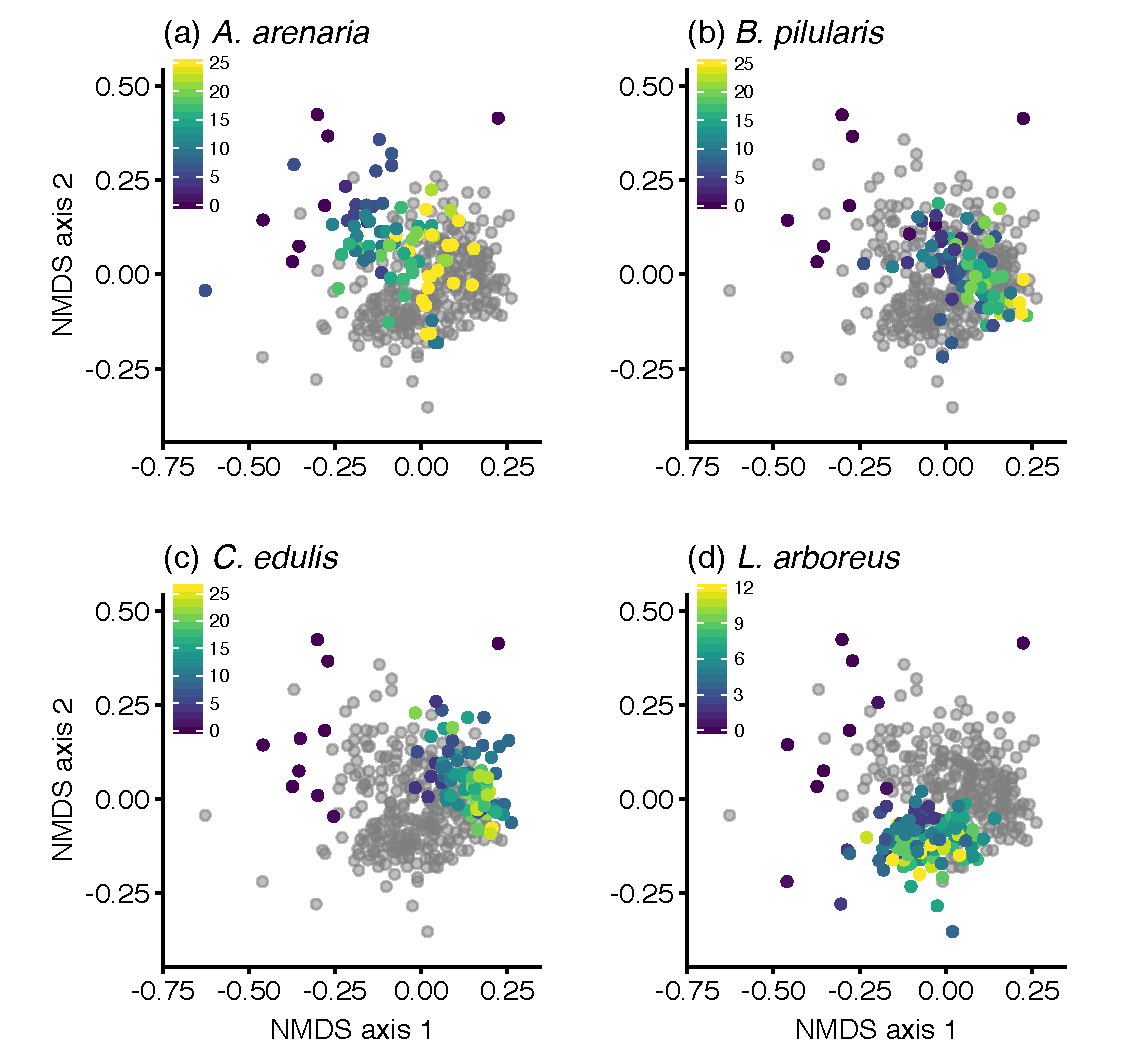
\includegraphics[width=14cm]{Chapter6/Composition_Fungi_Age.pdf}}
	\caption[Fungal community composition as a function of plant species and the age of plant individuals.]
		{\hspace{1mm} 
		Fungal community composition as a function of plant species and the age of plant individuals. Each panel highlights one focal plant species on the NMDS ordination plot of all fungal communities. Fungal communities associated with the focal species are color-coded by individual plant age, whereas the other three species are in gray. Purple to yellow represent the age gradient from young to old, with species-specific minimum and maximum age. (a) \textit{A. arenaria}; (b) \textit{B. pilularis}; (c) \textit{C. edulis}; (d) \textit{L. arboreus}. 
		Statistics were performed at the plant individual level, but for visualization purpose each point represents the fungal community of one soil sample. Note that dark purple points that appeared in all panels represent fungal communities associated with bare sand. See the same ordination plot but color-coded with species identity in Fig.~\ref{fig:BothComposition}a.}
	\label{fig:FunComposition}
\end{figure}



\newpage
\begin{figure}[h]
	\centering
	\makebox[\textwidth][c]{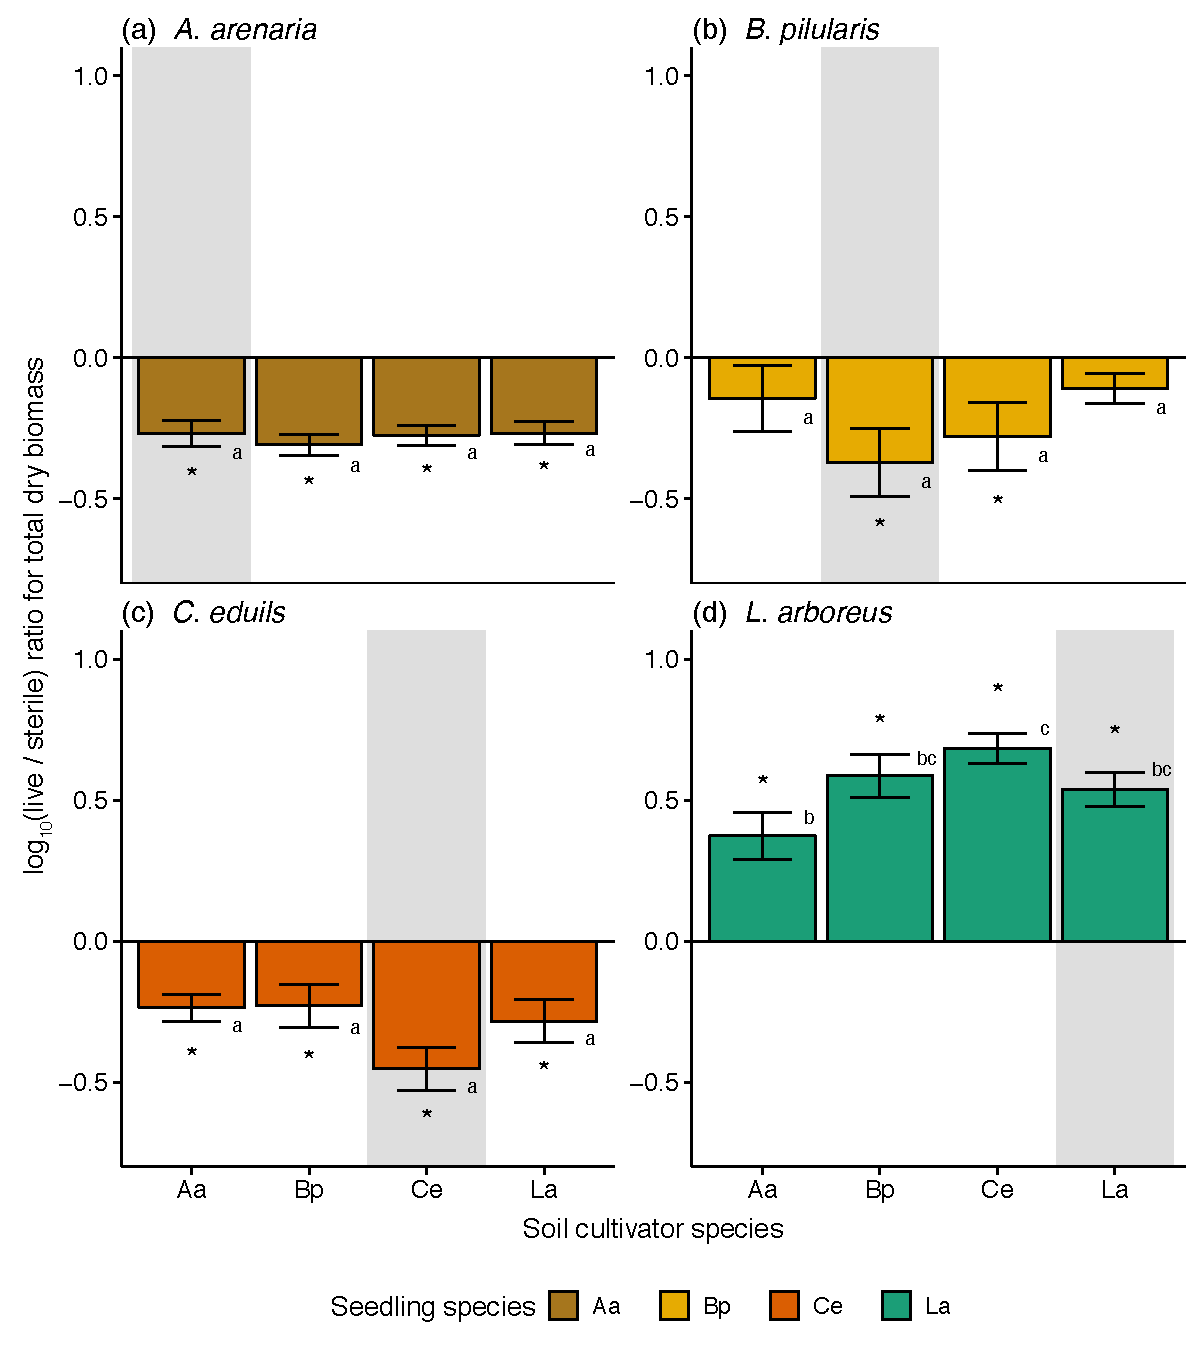
\includegraphics[width=14cm]{Chapter6/LiveSterRatioBarplot_Revised.pdf}}
	\caption[Mean ($\pm$ SE) microbial effects for each plant species in soils conditioned by different plants, neglecting the effects of soil conditioning length.]
		{\hspace{1mm} 
		Mean ($\pm$ SE) microbial effects for each plant species in soils conditioned by different plants, neglecting the effects of soil conditioning length. 
		(a) \textit{A. arenaria} (brown); (b) \textit{B. pilularis} (yellow); (c) \textit{C. edulis} (orange); (d) \textit{L. arboreus} (green). 
		The x-axis represents the plant species that conditioned the soil: \textit{A. arenaria} (Aa), \textit{B. pilularis} (Bp), \textit{C. edulis} (Ce), and \textit{L. arboreus} (La). The y-axis represents the microbial effects, defined as the log-ratio of plant total biomass in live soil and sterile soil, imposed by the soil host species. 
		Shaded bars represent conspecific microbial effects. Asterisks indicate microbial effects that are significantly different from zero, and different letters represent significant difference among the plant $\times$ soil host species combinations.}
	\label{fig:PSFBar}
\end{figure}



\newpage
\begin{figure}[h]
	%\vspace*{-1.0cm}
	\centering
	\makebox[\textwidth][c]{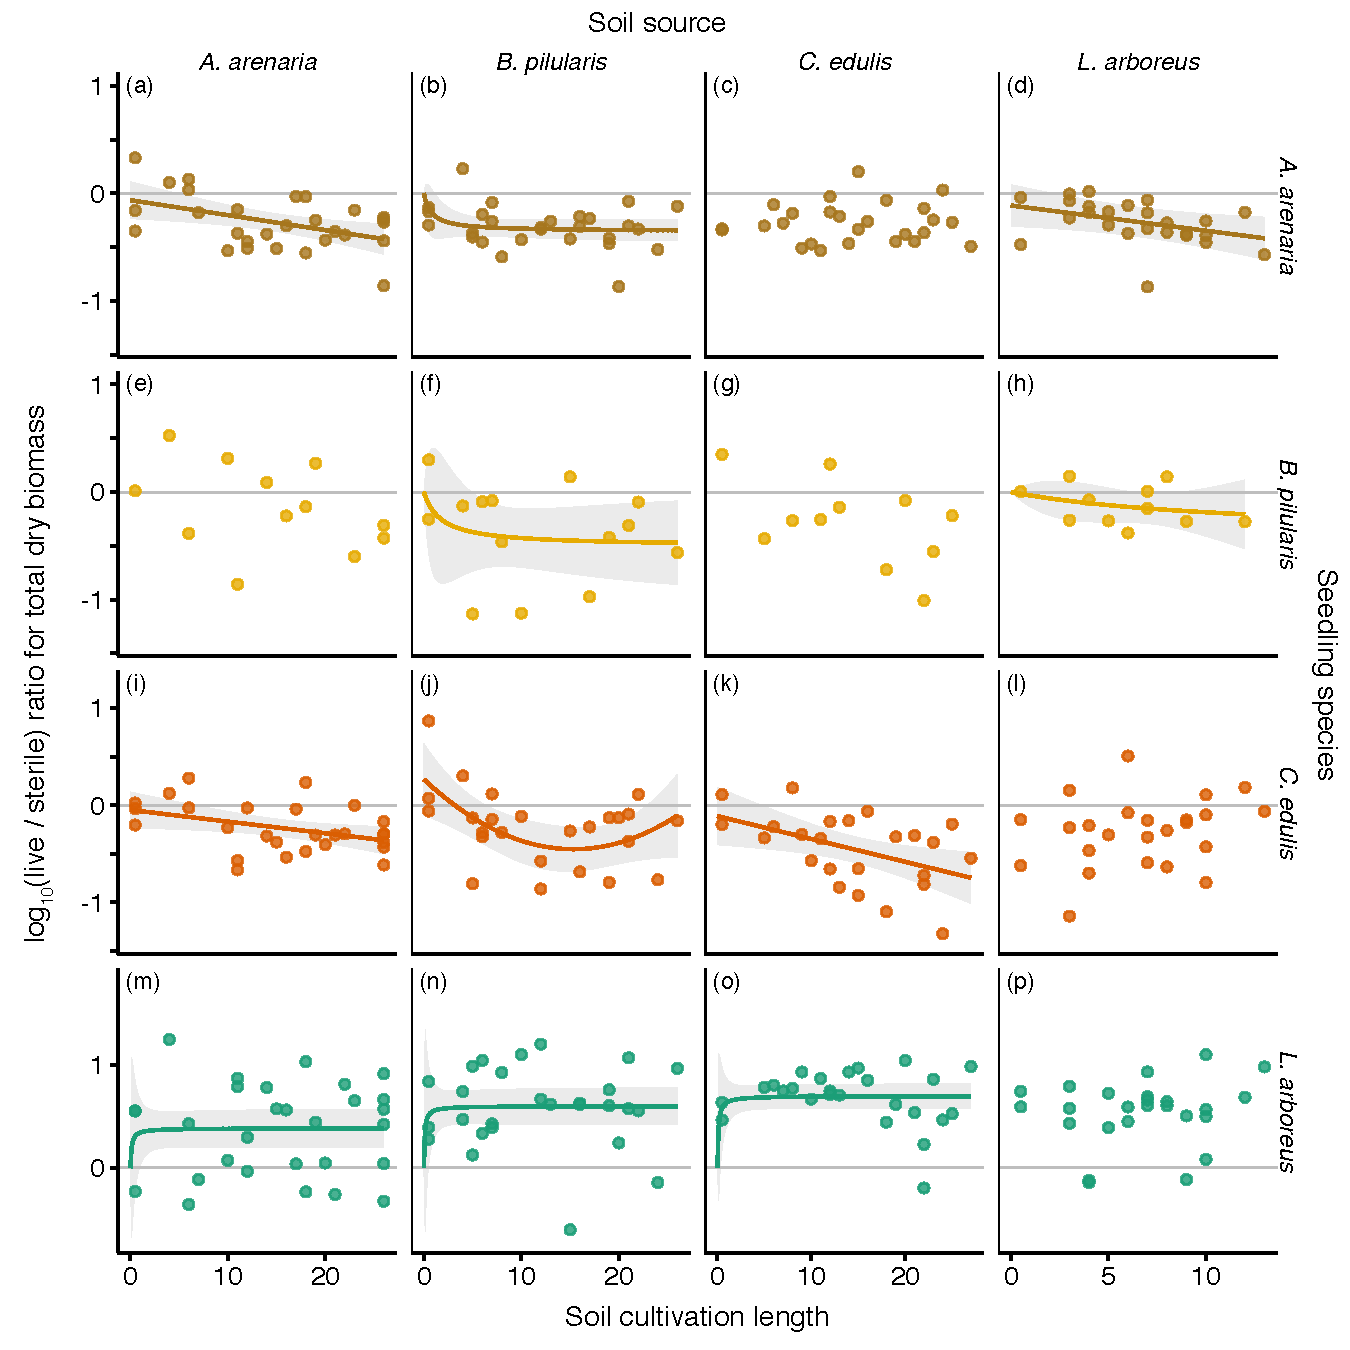
\includegraphics[width=14cm]{Chapter6/TemporalLiveSterRatio_Saturating_Revised.pdf}}
	\caption[Temporal trends of microbial effects for each plant $\times$ soil host species combination.]
		{\hspace{1mm} 
		Temporal trends of microbial effects for each plant (row) $\times$ soil host species (column) combination.
		Each point represents the microbial effect generated by soils collected from one plant individual.
		The x-axis represents the age of the plant individual that conditioned the soil, with maximum age up to 25 years old for \textit{A. arenaria} (first column), \textit{B. pilularis} (second column), and \textit{C. edulis} (third column), and up to 13 years old for \textit{L. arboreus} (fourth column). The y-axis represents the microbial effects imposed by the conditioning species, defined as the log-ratio of plant total biomass in live soil and sterile soil. The horizontal gray line in each panel represents no microbial effects.
		Colors/rows represent different plant species: \textit{A. arenaria} (brown, first row), \textit{B. pilularis} (yellow, second row), \textit{C. edulis} (orange, third row), and \textit{L. arboreus} (green, fourth row). The first three rows are plotted on the same scale.
		For each plant $\times$ soil host species combination, a fitted temporal trend line (and 95$\%$ confidence interval) is added if the length of soil conditioning affected the microbial effects (see main text for model fitting procedure).
		Note for combinations where the length of soil conditioning had little influence (i.e., no fitted trend line was added), its time-averaged microbial effects might still be significantly different from zero (see Fig.~\ref{fig:PSFBar}).}
	\label{fig:PSFTemporal}
\end{figure}



\newpage
\begin{figure}[h]
	\centering
	\makebox[\textwidth][c]{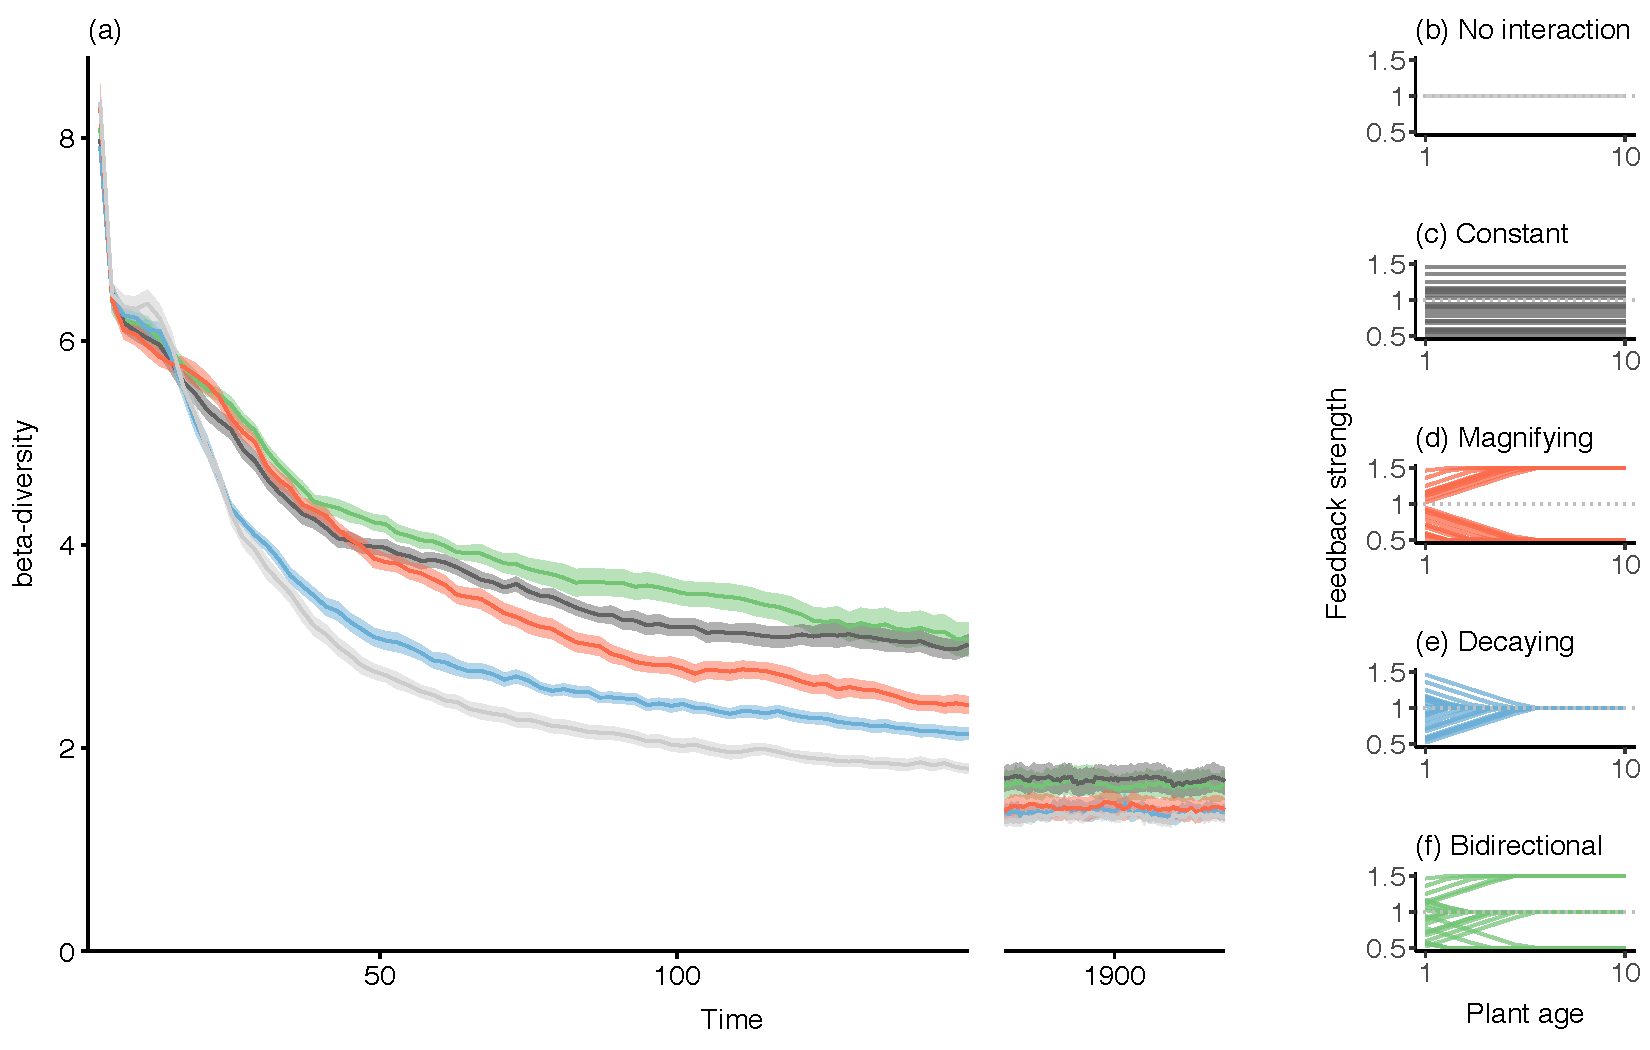
\includegraphics[width=15cm]{Chapter6/Simulation_ComplexPSF_Aggregate.pdf}}
	\caption[Simulated community convergence patterns under different temporal development scenarios of the underlying plant--soil microbe interactions.]
		{\hspace{1mm} 
		Simulated community convergence patterns under different temporal development scenarios of the underlying plant--soil microbe interactions.
		(a) Temporal trends of beta-diversity (mean $\pm$ SE, $n = 20$) among the 10 simulated patches for five different plant--soil microbe interaction scenarios. (b)--(f) Schematic diagrams of the five different scenarios in (a), demonstrating how the interaction strength changes with the age of the conditioning individual.
		(b) No plant--soil microbe interactions (light gray); (c) Plant--soil microbe interactions that are independent to plant age (black); (d) Magnifying interaction strengths that intensify to their biological extremes with increasing plant age (orange); (e) Decaying interaction strengths that attenuate to one with increasing plant age (blue); (f) Bidirectionally varying interaction strengths that either intensify or attenuate with increasing plant age (green). See Appendix E.1 for detailed model description.}
	\label{fig:SimulationComplexPSF}
\end{figure}





%% END MATERIAL
\appendix
\chapter{Linking modern coexistence theory and contemporary niche theory: Appendices S1--S5}
%\chaptermark{Niche and coexistence theory}
%\renewcommand{\sectionmark}[1]{}
\fancyhead[LE, RO]{\thepage}
\fancyhead[RE]{APPENDIX A}
\fancyhead[LO]{NICHE AND COEXISTENCE THEORY}
\fancyfoot{}
\renewcommand{\headrulewidth}{0pt}
\setlength{\parindent}{1cm}


\begin{comment}
\documentclass[hidelinks,12pt]{article}
\usepackage{graphicx,bm, booktabs,lineno,array}
\usepackage[fleqn]{amsmath}
\setlength{\mathindent}{0pt}
\usepackage[compress,comma]{natbib}
\usepackage[a4paper]{geometry}
\usepackage[parfill]{parskip}
\usepackage[usenames,dvipsnames]{color}
\usepackage[font=large,labelfont=bf,margin=1cm, labelsep = none]{caption} % caption formatting
\usepackage{setspace}
\usepackage{gensymb}
\usepackage{color} 
\usepackage{sidecap}
\usepackage{etoolbox}
\newbool{MyRefNumbers}
\usepackage{authblk}
\usepackage{hyperref}
\usepackage[color=cyan]{todonotes}
\pdfminorversion=3
\doublespacing

\newcommand{\plus}{\raisebox{.4\height}{\scalebox{.6}{+}}}
\newcommand{\minus}{\raisebox{.4\height}{\scalebox{.8}{-}}}
\newcommand*\samethanks[1][\value{footnote}]{\footnotemark[#1]}
\newcommand\blfootnote[1]{%
  \begingroup
  \renewcommand\thefootnote{}\footnote{#1}%
  \addtocounter{footnote}{-1}%
  \endgroup
}
\end{comment}



\begin{comment}
\title{Linking modern coexistence theory and contemporary niche theory}
\author[1]{Andrew D. Letten \thanks{These authors contributed equally.}}
\author[1]{Po-Ju Ke \samethanks}
\author[1]{Tadashi Fukami}
\affil[1]{Department of Biology, Stanford University, Stanford, California, 94305-5020, USA}

\begin{document}

\date{}
\maketitle
\singlespacing
\blfootnote{Correspondence email: aletten@stanford.edu, pojuke@stanford.edu, fukamit@stanford.edu}
\textbf{Type of article:} Concepts and Synthesis
\textbf{Running title:} Niche and coexistence theory 
\textbf{Figures:} 6\\
\textbf{Boxes:} 2\\
\newpage
\doublespacing
\linenumbers
\end{comment}



\section{Appendix S1}
To analytically link modern coexistence theory \citep{Chesson2000} and contemporary niche theory \citep{Chase2003}, we translated consumer-resource models into a Lotka--Volterra form following \cite[Ch.~7]{tilman1982}. For a Lotka--Volterra competition model for two consumer species (i.e., $N_{1}$ and $N_{2}$) written as

\begin{equation}
\frac{dN_{1}}{dt}=r_{1}N_{1}\left ( 1-a_{11}N_{1}-a_{12}N_{2} \right ) 
\tag{S2.1.1}\label{eq:S2.1.1}
\end{equation}
\begin{equation}
\frac{dN_{2}}{dt}=r_{2}N_{2}\left ( 1-a_{21}N_{1}-a_{22}N_{2} \right ). 
\tag{S2.1.2}\label{eq:S2.1.2}
\end{equation}

\noindent The model will have an equilibrium density when $N_{1}^{*}=\frac{1}{a_{11}}-\frac{a_{12}}{a_{11}}N_{2}^{*}$ and $N_{2}^{*}=\frac{1}{a_{22}}-\frac{a_{21}}{a_{22}}N_{1}^{*}$. \cite{tilman1982} solved the equilibrium of the consumer-resource model and rearranged it algebraically to a form that is comparable to the equilibrium of a Lotka--Volterra model (an alternative approach to translating consumer-resource models to Lotka--Volterra form involves linearizing inter- and intraspecific density dependences at the equilibrium \citep{Meszenaz2006}, as recently applied in \cite{Kleinhesselink2015}). Note that \cite{tilman1982} parameterized the Lotka--Volterra model in terms of carrying capacities (i.e., $K_{1}$ and $K_{2}$) and relative competition coefficients (i.e., $\alpha$ and $\beta$). His derivation allowed for the rewriting of these parameters in terms of consumer-resource parameters. 
\par


In this appendix, we provide detailed mathematical derivations for two species competing for both perfectly substitutable resources and essential resources. To maintain consistency with modern coexistence theory, we parameterized the Lotka--Volterra model using absolute competition coefficients (i.e., $a_{ij}$). Once the consumer-resource model was translated to a Lotka--Volterra form, we were able to go one step further to quantify Chesson's niche overlap and average fitness difference \citep{Chesson2000, Godoy2014}. 
\par


\subsection{Mathematical derivation of Chesson's niche overlap and fitness differences for two consumers competing for two substitutable resources}
Following \citet[p.~270]{tilman1982}, the model consists of two resources (i.e., $R_{1}$ and $R_{2}$) that are perfectly nutritionally substitutable for two consumers (i.e., $N_{1}$ and $N_{2}$): 

\begin{equation}
\frac{{d{N_1}}}{{dt}} = {r_1}{N_1}\left[ {\frac{{{w_{11}}{R_1} + {w_{12}}{R_2} - {T_1}}}{{{k_1} + {w_{11}}{R_1} + {w_{12}}{R_2} - {T_1}}}} \right] - D{N_1} 
\tag{S2.2.1}\label{eq:S2.2.1}
\end{equation}
\begin{equation}
\frac{{d{N_2}}}{{dt}} = {r_2}{N_2}\left[ {\frac{{{w_{21}}{R_1} + {w_{22}}{R_2} - {T_2}}}{{{k_2} + {w_{21}}{R_1} + {w_{22}}{R_2} - {T_2}}}} \right] - D{N_2} 
\tag{S2.2.2}\label{eq:S2.2.2}
\end{equation}
\begin{equation}
\frac{{d{R_1}}}{{dt}} = D\left( {{S_1} - {R_1}} \right) - {c_{11}}{N_1} - {c_{21}}{N_2} \tag{S2.2.3}\label{eq:S2.2.3}
\end{equation}
\begin{equation}
\frac{{d{R_2}}}{{dt}} = D\left( {{S_2} - {R_2}} \right) - {c_{12}}{N_1} - {c_{22}}{N_2}.
\tag{S2.2.4}\label{eq:S2.2.4}
\end{equation}

\noindent Here, $r_{i}$ represents the maximum population growth rate for species $i$ ($i = $ 1 or 2) and $D$ represents the constant mortality of the consumers and turnover rate of resources. Per capita resource consumption rate of consumer $N_{i}$ on resource $R_{j}$ ($j = $ 1 or 2) is represented by $c_{ij}$, whereas $w_{ij}$ represents a weighting factor that converts availability of $R_{j}$ into its value for consumer $N_{i}$. Following a Monod growth model, $k_{i}$ is the half-saturation constant for $N_{i}$ resource consumption, and $T_{i}$ is the minimum amount of total resource required for $N_{i}$ to grow. Finally, $S_{1}$ and $S_{2}$ represent the resource supply concentrations for $R_{1}$ and $R_{2}$, respectively. As noted in \cite{Kleinhesselink2015}, certain assumptions of this Monod growth model, such as constant supply of resource and strong recipient control of consumption rate, may not be applicable to many systems. However, this should not affect the results qualitatively.
\par


By setting Eqns.~\ref{eq:S2.2.1} and \ref{eq:S2.2.2} to zero, we solved the zero net growth isolines (ZNGI) of consumers, which represent resource combinations of $R_{1}$ and $R_{2}$ that cause consumers' growth equal to its mortality, as:

\begin{equation}
R_2 =  - \frac{{{w_{11}}}}{{{w_{12}}}}R_1 + {B_1} 
\tag{S2.3.1}\label{eq:S2.3.1}
\end{equation}
\begin{equation}
R_2 =  - \frac{{{w_{21}}}}{{{w_{22}}}}R_1 + {B_2}, 
\tag{S2.3.2}\label{eq:S2.3.2}
\end{equation}

\noindent where ${B_1} = \left[ {\frac{{D\left( {{k_1} - {T_1}} \right) + {r_1}{T_1}}}{{{w_{12}}\left( {{r_1} - D} \right)}}} \right]$, and ${B_2} = \left[ {\frac{{D\left( {{k_2} - {T_2}} \right) + {r_2}{T_2}}}{{{w_{21}}\left( {{r_2} - D} \right)}}} \right]\left( {\frac{{{w_{21}}}}{{{w_{22}}}}} \right)$. Given that the ZNGI of $N_{1}$ and $N_{2}$ must cross to ensure coexistence of consumers, the equilibrium resource densities, $R_{1}^{*}$ and $R_{2}^{*}$, were solved as:

\begin{equation}
R_1^* = {{\left( {{B_1} - {B_2}} \right)} \mathord{\left/
		{\vphantom {{\left( {{B_1} - {B_2}} \right)} {\left( {\frac{{{w_{11}}}}{{{w_{12}}}} - \frac{{{w_{21}}}}{{{w_{22}}}}} \right)}}} \right.
		\kern-\nulldelimiterspace} {\left( {\frac{{{w_{11}}}}{{{w_{12}}}} - \frac{{{w_{21}}}}{{{w_{22}}}}} \right)}} 
\tag{S2.4.1}\label{eq:S2.4.1}
\end{equation}
\begin{equation}
R_2^* = {{\left( {{B_1}\frac{{{w_{12}}}}{{{w_{11}}}} - {B_2}\frac{{{w_{22}}}}{{{w_{21}}}}} \right)} \mathord{\left/
		{\vphantom {{\left( {{B_1}\frac{{{w_{12}}}}{{{w_{11}}}} - {B_2}\frac{{{w_{22}}}}{{{w_{21}}}}} \right)} {\left( {\frac{{{w_{21}}}}{{{w_{11}}}} - \frac{{{w_{22}}}}{{{w_{21}}}}} \right)}}} \right.
		\kern-\nulldelimiterspace} {\left( {\frac{{{w_{12}}}}{{{w_{11}}}} - \frac{{{w_{22}}}}{{{w_{21}}}}} \right)}}.
\tag{S2.4.2}\label{eq:S2.4.2}
\end{equation}

\noindent By substituting the equilibrium resource densities into Eqns.~\ref{eq:S2.2.3} and \ref{eq:S2.2.4}, we obtained the equilibrium consumer densities, $N_{1}^{*}$ and $N_{2}^{*}$. The consumer equilibrium density can be written in a form comparable to that of the Lotka--Volterra model. For $N_{1}$, the specific form of its equilibrium density can be derived by Eqn.~\ref{eq:S2.2.3} $\times \frac{w_{11}}{w_{12}} + $ Eqn.~\ref{eq:S2.2.4}:

\begin{equation}
N_1^* = \left[ {\frac{{D\left( {{S_2} + \frac{{{w_{11}}}}{{{w_{12}}}}{S_1} - {B_1}} \right)}}{{{c_{12}} + {c_{11}}\frac{{{w_{11}}}}{{{w_{12}}}}}}} \right] - \left[ {\frac{{{c_{22}} + {c_{21}}\frac{{{w_{11}}}}{{{w_{12}}}}}}{{{c_{12}} + {c_{11}}\frac{{{w_{11}}}}{{{w_{12}}}}}}} \right]N_2^*. 
\tag{S2.5}\label{eq:S2.5}
\end{equation}

Eqn.~\ref{eq:S2.5} consists of a first component with only $N_{1}$-related parameters, and a heterospecific density-dependent component which decreases with its competitor's density (i.e., $N_{2}^{*}$). Note that the specific algebraic treatment applied to obtain Eqn.~\ref{eq:S2.5} served the purpose to generate the density-independent component independent of parameters of the competitor. By comparing this expression with $N_{1}^{*}=\frac{1}{a_{11}}-\frac{a_{12}}{a_{11}}N_{2}^{*}$, the algebraic equivalents for $a_{11}$ and $a_{12}$ are:

\begin{equation}
{a_{11}} = \frac{{{c_{12}} + {c_{11}}\frac{{{w_{11}}}}{{{w_{12}}}}}}{{D\left( {{S_2} + \frac{{{w_{11}}}}{{{w_{12}}}}{S_1} - {B_1}} \right)}}
\tag{S2.6.1}\label{eq:S2.6.1}
\end{equation}
\begin{equation}
{a_{12}} = \frac{{{c_{22}} + {c_{21}}\frac{{{w_{11}}}}{{{w_{12}}}}}}{{D\left( {{S_2} + \frac{{{w_{11}}}}{{{w_{12}}}}{S_1} - {B_1}} \right)}}.
\tag{S2.6.2}\label{eq:S2.6.2}
\end{equation}

\noindent For $N_{2}$, its equilibrium density can be derived by Eqn.~\ref{eq:S2.2.3}$\times \frac{w_{21}}{w_{22}} + $ Eqn.~\ref{eq:S2.2.4}:

\begin{equation}
N_2^* = \left[ {\frac{{D\left( {{S_2} + \frac{{{w_{21}}}}{{{w_{22}}}}{S_1} - {B_2}} \right)}}{{{c_{22}} + {c_{21}}\frac{{{w_{21}}}}{{{w_{22}}}}}}} \right] - \left[ {\frac{{{c_{12}} + {c_{11}}\frac{{{w_{21}}}}{{{w_{22}}}}}}{{{c_{22}} + {c_{21}}\frac{{{w_{21}}}}{{{w_{22}}}}}}} \right]N_1^*.
\tag{S2.7}\label{eq:S2.7}
\end{equation}

Similar to Eqn.~\ref{eq:S2.5}, Eqn.~\ref{eq:S2.7} consists of a density-independent component with only $N_{2}$-related parameters, and a heterospecific density-dependent component which decreases with the density of $N_{1}^{*}$. By comparing Eqn.~\ref{eq:S2.7} with $N_{2}^{*}=\frac{1}{a_{22}}-\frac{a_{21}}{a_{22}}N_{1}^{*}$, the algebraic equivalents for $a_{22}$ and $a_{21}$ are:

\begin{equation}
{a_{22}} = \frac{{{c_{22}} + {c_{21}}\frac{{{w_{21}}}}{{{w_{22}}}}}}{{D\left( {{S_2} + \frac{{{w_{21}}}}{{{w_{22}}}}{S_1} - {B_2}} \right)}} 
\tag{S2.8.1}\label{eq:S2.8.1}
\end{equation}
\begin{equation}
{a_{21}} = \frac{{{c_{12}} + {c_{11}}\frac{{{w_{21}}}}{{{w_{22}}}}}}{{D\left( {{S_2} + \frac{{{w_{21}}}}{{{w_{22}}}}{S_1} - {B_2}} \right)}}.
\tag{S2.8.2}\label{eq:S2.8.2}
\end{equation}

Chesson defines niche overlap as $\rho=\sqrt {\frac{{{a_{12}}{a_{21}}}}{{{a_{11}}{a_{22}}}}}$ and absolute fitness difference of $N_{2}$ over $N_{1}$ as $\frac{{{f_2}}}{{{f_1}}} = \sqrt {\frac{{{a_{11}}{a_{12}}}}{{{a_{22}}{a_{21}}}}}$ \citep{Chesson2013ecosys}. By writing out the absolute competition coefficients in terms of consumer-resource parameters (i.e., Eqns.~\ref{eq:S2.6.1} -- \ref{eq:S2.6.2} and Eqns.~\ref{eq:S2.8.1} -- \ref{eq:S2.8.2}), we can express the niche overlap as: 

\begin{equation}
\rho  = \sqrt {\frac{{{a_{12}}{a_{21}}}}{{{a_{11}}{a_{22}}}}}  = \sqrt {\frac{\left (
		c_{22} + c_{21}\frac{w_{11}}{w_{12}}\right )\left ( 
		c_{12} + c_{11}\frac{w_{21}}{w_{22}} \right )}{\left (
		c_{12} + c_{11}\frac{w_{11}}{w_{12}}\right )\left ( 
		c_{22} + c_{21}\frac{w_{21}}{w_{22}} \right )}} 
\tag{S2.9}\label{eq:S2.9}
\end{equation}
and the absolute fitness difference of $N_{2}$ over $N_{1}$ as:
\begin{equation}
\frac{{{f_2}}}{{{f_1}}} = \sqrt {\frac{{{a_{11}}{a_{12}}}}{{{a_{22}}{a_{21}}}}}  = \frac{\left (S_{2}+\frac{w_{21}}{w_{22}}S_{1}-B_{2}\right )}{\left (S_{2}+\frac{w_{11}}{w_{12}}S_{1}-B_{1}\right )}\sqrt {\frac{\left (
		c_{12} + c_{11}\frac{w_{11}}{w_{12}}\right )\left ( 
		c_{22} + c_{21}\frac{w_{11}}{w_{12}} \right )}{\left (
		c_{22} + c_{21}\frac{w_{21}}{w_{22}}\right )\left ( 
		c_{12} + c_{11}\frac{w_{21}}{w_{22}} \right )}}.
\tag{S2.10}\label{eq:2.10}
\end{equation}


\subsection{Mathematical derivation of Chesson's niche overlap and fitness differences for two consumers competing for two essential resources} 
We applied the same mathematical techniques for a consumer-resource model where the resources are essential, which takes the general form as follows \citep{tilman1982}: 

\begin{equation}
\frac{{d{N_1}}}{{dt}} = {r_1}{N_1}\min \left[ {\frac{{{R_1}}}{{{R_1} + {k_{11}}}},{\rm{ }}\frac{{{R_2}}}{{{R_2} + {k_{12}}}}} \right] - {m_1}{N_1} 
\tag{S2.11.1}\label{eq:S2.11.1}
\end{equation}
\begin{equation}
\frac{{d{N_2}}}{{dt}} = {r_2}{N_2}\min \left[ {\frac{{{R_1}}}{{{R_1} + {k_{21}}}},{\rm{ }}\frac{{{R_2}}}{{{R_2} + {k_{22}}}}} \right] - {m_2}{N_2}
\tag{S2.11.2}\label{eq:S2.11.2}
\end{equation}
\begin{equation}
\frac{{d{R_1}}}{{dt}} = D\left( {{S_1} - {R_1}} \right) - {c_{11}}\left( {\frac{{d{N_1}}}{{dt}} + {m_1}{N_1}} \right) - {c_{21}}\left( {\frac{{d{N_2}}}{{dt}} + {m_2}{N_2}} \right)
\tag{S2.11.3}\label{eq:S2.11.3}
\end{equation}
\begin{equation}
\frac{{d{R_2}}}{{dt}} = D\left( {{S_2} - {R_2}} \right) - {c_{12}}\left( {\frac{{d{N_1}}}{{dt}} + {m_1}{N_1}} \right) - {c_{22}}\left( {\frac{{d{N_2}}}{{dt}} + {m_2}{N_2}} \right).
\tag{S2.11.4}\label{eq:S2.11.4}
\end{equation}

\noindent Here, $m_1$ and $m_2$ represent mortality rates for consumers $N_1$ and $N_2$, respectively, whereas other parameter notations are the same as Eqns.~\ref{eq:S2.2.1} -- \ref{eq:S2.2.4}. In order to keep consistency with \cite[Ch.~7]{tilman1982}, we applied the following specific model for our analysis:  

\begin{equation}
\frac{{d{N_1}}}{{dt}} = {r_1}{N_1}\min \left[ {\frac{{{R_1}}}{{{R_1} + {k_{11}}}},{\rm{ }}\frac{{{R_2}}}{{{R_2} + {k_{12}}}}} \right] - {m_1}{N_1}
\tag{S2.12.1}\label{eq:S2.12.1}
\end{equation}
\begin{equation}
\frac{{d{N_2}}}{{dt}} = {r_2}{N_2}\min \left[ {\frac{{{R_1}}}{{{R_1} + {k_{21}}}},{\rm{ }}\frac{{{R_2}}}{{{R_2} + {k_{22}}}}} \right] - {m_2}{N_2}
\tag{S2.12.2}\label{eq:S2.12.2}
\end{equation}
\begin{equation}
\frac{{d{R_1}}}{{dt}} = D\left( {{S_1} - {R_1}} \right) - {c_{11}}{N_{1}} - {c_{21}}{N_{2}}
\tag{S2.12.3}\label{eq:S2.12.3}
\end{equation}
\begin{equation}
\frac{{d{R_2}}}{{dt}} = D\left( {{S_2} - {R_2}} \right) - {c_{12}}{N_{1}} - {c_{22}}{N_{2}}.
\tag{S2.12.4}\label{eq:S2.12.4}
\end{equation}

\noindent As mentioned in the main text, nutrient limitation status due to resource availability depends on the relative position of the resource supply point, the monocultural resource equilibrium (i.e., $R_{ij}^{*}$), and the consumption vector. When translating the essential consumer-resource model to Lotka--Volterra form, we thus need to consider the nutrient limitation status of each species (Fig.~\ref{fig:supply-ms-fig}c). By drawing a line from each species' $R_{ij}^{*}$ parallel to its consumption vector, we can partition the resource supply space into three sections: (i) both $N_{1}$ and $N_{2}$ are limited by $R_{1}$ (i.e., beyond the blue dotted lines), (ii) $N_{1}$ is limited by $R_{2}$ and $N_{2}$ is limited by $R_{1}$ (i.e., between the blue and red dotted line), and (iii) both $N_{1}$ and $N_{2}$ are limited by $R_{2}$ (i.e., below the red dotted lines) (Fig.~\ref{fig:supply-ms-fig}c). Here, we demonstrate how Chesson's niche overlap and fitness difference can be quantified in an essential resource model by focusing on region (ii), where the two species are limited by different resources at the equilibrium. In this region, Eqns.~\ref{eq:S2.12.1} -- \ref{eq:S2.12.4} becomes:

\begin{equation}
\frac{{d{N_1}}}{{dt}} = {r_1}{N_1} \left[{\frac{{{R_2}}}{{{R_2} + {k_{12}}}}} \right] - {m_1}{N_1}
\tag{S2.13.1}\label{eq:S2.13.1}
\end{equation}
\begin{equation}
\frac{{d{N_2}}}{{dt}} = {r_2}{N_2} \left[{\frac{{{R_1}}}{{{R_1} + {k_{21}}}}} \right] - {m_2}{N_2}
\tag{S2.13.2}\label{eq:S2.13.2}
\end{equation}
\begin{equation}
\frac{{d{R_1}}}{{dt}} = D\left( {{S_1} - {R_1}} \right) - {c_{11}}{N_{1}} - {c_{21}}{N_{2}}
\tag{S2.13.3}\label{eq:S2.13.3}
\end{equation}
\begin{equation}
\frac{{d{R_2}}}{{dt}} = D\left( {{S_2} - {R_2}} \right) - {c_{12}}{N_{1}} - {c_{22}}{N_{2}}.
\tag{S2.13.4}\label{eq:S2.13.4}
\end{equation}

As in the substitutable resource model, we solved for the equilibrium resource densities. While this is represented as the ZNGI in the substitutable resource model, here we can directly solve for $R_{2}^{*}$ (defined as $R_{12}^{*}$) from Eqn.~\ref{eq:S2.13.1} and $R_{1}^{*}$ (defined as $R_{21}^{*}$) from Eqn.~\ref{eq:S2.13.2} as:

\begin{equation}
R_{12}^{*}=\frac{m_{1}k_{12}}{r_{1}-m_{1}}
\tag{S2.14.1}\label{eq:S2.14.1}
\end{equation}
\begin{equation}
R_{21}^{*}=\frac{m_{2}k_{21}}{r_{2}-m_{2}}.
\tag{S2.14.2}\label{eq:S2.14.2}
\end{equation}

Substituting Eqns.~\ref{eq:S2.14.1} and \ref{eq:S2.14.2} back to Eqns.~\ref{eq:S2.13.3} and \ref{eq:S2.13.4} respectively allows us to solve the equilibrium for $N_{1}$ and $N_{2}$ as:

\begin{equation}
N_{1}^{*}=\frac{D}{c_{12}}\left ( S_{2}-{R_{12}^{*}} \right )-\frac{c_{22}}{c_{12}}N_{2}^{*}
\tag{S2.15.1}\label{eq:S2.15.1}
\end{equation}
\begin{equation}
N_{2}^{*}=\frac{D}{c_{21}}\left ( S_{1}-{R_{21}^{*}} \right )-\frac{c_{11}}{c_{21}}N_{1}^{*}.
\tag{S2.15.2}\label{eq:S2.15.2}
\end{equation}

\noindent By comparing Eqns.\ref{eq:S2.15.1} and \ref{eq:S2.15.2} to $N_{1}^{*}=\frac{1}{a_{11}}-\frac{a_{12}}{a_{11}}N_{2}^{*}$ and $N_{2}^{*}=\frac{1}{a_{22}}-\frac{a_{21}}{a_{22}}N_{1}^{*}$, respectively, we find $a_{11}$, $a_{12}$, $a_{21}$, and $a_{22}$ for the essential resource model in region (ii):

\begin{equation}
a_{11}=\frac{c_{12}}{D\left ( S_{2}-R_{12}^{*} \right )}
\tag{S2.16.1}\label{eq:S2.16.1}
\end{equation}
\begin{equation}
a_{12}=\frac{c_{22}}{D\left ( S_{2}-R_{12}^{*} \right )}
\tag{S2.16.2}\label{eq:S2.16.2}
\end{equation}
\begin{equation}
a_{21}=\frac{c_{11}}{D\left ( S_{1}-R_{21}^{*} \right )}
\tag{S2.16.3}\label{eq:S2.16.3}
\end{equation}
\begin{equation}
a_{22}=\frac{c_{21}}{D\left ( S_{1}-R_{21}^{*} \right )}.
\tag{S2.16.4}\label{eq:S2.16.4}
\end{equation}

\noindent Following similar methods, we solved for each of Chesson's components in regions where both species are limited by the same resource. For region (i), where both species are $R_{1}$-limited, 

\begin{equation}
a_{11}=\frac{c_{11}}{D\left ( S_{1}-R_{11}^{*} \right )}
\tag{S2.17.1}\label{eq:S2.17.1}
\end{equation} 
\begin{equation}
a_{12}=\frac{c_{21}}{D\left ( S_{1}-R_{11}^{*} \right )}
\tag{S2.17.2}\label{eq:S2.17.2} 
\end{equation}
\begin{equation}
a_{21}=\frac{c_{11}}{D\left ( S_{1}-R_{21}^{*} \right )}
\tag{S2.17.3}\label{eq:S2.17.3}
\end{equation}
\begin{equation}
a_{22}=\frac{c_{21}}{D\left ( S_{1}-R_{21}^{*} \right )}.
\tag{S2.17.4}\label{eq:S2.17.4}
\end{equation}

\noindent For region (iii), where both species are $R_{2}$-limited, 

\begin{equation}
a_{11}=\frac{c_{12}}{D\left ( S_{2}-R_{12}^{*} \right )}
\tag{S2.18.1}\label{eq:S2.18.1}
\end{equation}
\begin{equation}
a_{12}=\frac{c_{22}}{D\left ( S_{2}-R_{12}^{*} \right )}
\tag{S2.18.2}\label{eq:S2.18.2}
\end{equation}
\begin{equation}
a_{21}=\frac{c_{12}}{D\left ( S_{2}-R_{22}^{*} \right )}
\tag{S2.18.3}\label{eq:S2.18.3}
\end{equation}
\begin{equation}
a_{22}=\frac{c_{22}}{D\left ( S_{2}-R_{22}^{*} \right )}.
\tag{S2.18.4}\label{eq:S2.18.4}
\end{equation}



\section{Appendix S2}
In this study we used Tilman's consumer-resource model for substitutable resources (i.e., Appendix A, Eqns.~\ref{eq:S2.2.1} -- \ref{eq:S2.2.4}) following \cite[p.~270]{tilman1982}, which has also been applied in many other studies (e.g., \cite{Meszenaz2006}, \cite{Barabas2014}). As pointed out by \cite{Kleinhesselink2015}, this model assumes that resource uptake is proportional only to consumer abundance. The structure of this model may result in negative resource equilibrium values, especially under the scenario where one species excludes the other (i.e., the mono-dominance equilibrium). As mentioned in the main text, our simulations were performed in parameter regions that only resulted in positive resource equilibrium values. Here, we further supplement this argument with analytical solutions for this particular model. We first derived the analytical solution of the equilibrium when $N_1$ outcompetes $N_2$ (hereafter termed \textbf{$E_{N1}^{*}$}), and when $N_2$ outcompetes $N_1$ (hereafter termed \textbf{$E_{N2}^{*}$}). We then derived the criteria for positive resource equilibrium and listed the parameters used for the simulations. 
\par


\subsection{Analytical form and positivity criteria of $E_{N1}^{*}$} 
Under \textbf{$E_{N1}^{*}$} ($N_{1}^{*} >$  0, $N_{2}^{*}$ = 0), by setting Eqns.~\ref{eq:S2.2.3} and \ref{eq:S2.2.4} equal to zero, we derived Eqns.~\ref{eq:S2.19.1} and \ref{eq:S2.19.2}, respectively:

\begin{equation}
R_{1}^{*} = S_1-\frac{c_{11}}{D}N_{1}^{*}
\tag{S2.19.1}\label{eq:S2.19.1}
\end{equation}
\begin{equation}
R_{2}^{*} = S_2-\frac{c_{12}}{D}N_{1}^{*}.
\tag{S2.19.2}\label{eq:S2.19.2}
\end{equation}

\noindent By substituting Eqns.~\ref{eq:S2.19.1} and \ref{eq:S2.19.2} into Eqns.~\ref{eq:S2.2.1}, $N_{1}^{*}$ can be derived as follows:

\begin{equation}
N_{1}^{*} = D\left [\frac{\left ( r_1 - D\right )\left ( w_{11}S_{1}+w_{12}S_{2}-T_{1} \right )-Dk_{1}}{\left ( r_1-D \right )\left (  w_{11}c_{11}+w_{12}c_{12} \right )}\right].
\tag{S2.20}\label{eq:S2.20}
\end{equation}

\noindent For $R_{1}^{*}$ and $R_{2}^{*}$ to be positive, the following two inequalities should be fulfilled respectively:

\begin{equation}
S_1\left ( r_{1}-D \right )w_{12}c_{12} - S_2\left ( r_1-D \right )w_{12}c_{11} > -\left ( r_{1}-D \right )c_{11}T_{1} - Dk_{1}c_{11}
\tag{S2.21.1}\label{eq:S2.21.1}
\end{equation}
\begin{equation}
S_1\left ( r_{1}-D \right )w_{11}c_{12} - S_2\left ( r_1-D \right )w_{11}c_{11} < \left ( r_{1}-D \right )c_{12}T_{1} - Dk_{1}c_{12}.
\tag{S2.21.2}\label{eq:S2.21.2}
\end{equation}

By combining criteria \ref{eq:S2.21.1} and \ref{eq:S2.21.2}, we derived the criteria for positive resource equilibrium under $E_{N1}^{*}$:

\begin{equation}
\frac{-1}{w_{12}c_{12}}\left [ T_{1} + \frac{Dk_{1}}{\left ( r_{1}-D \right )}\right ] < \frac{S_1}{c_{11}}-\frac{S_2}{c_{12}} < \frac{1}{w_{11}c_{11}}\left [ T_{1} + \frac{Dk_{1}}{\left ( r_{1}-D \right )}\right ].
\tag{S2.22}\label{eq:S2.22}
\end{equation}



\subsection{Analytical form and positivity criteria of $E_{N2}^{*}$} 
Following similar mathematical logic, we derived the analytical form of $E_{N2}^{*}$ ($N_{1}^{*} =$  0, $N_{2}^{*} >$ 0) as follows:

\begin{equation}
N_{2}^{*} = D\left [\frac{\left ( r_2 - D\right )\left ( w_{21}S_{1}+w_{22}S_{2}-T_{2} \right )-Dk_{2}}{\left ( r_2-D \right )\left (  w_{21}c_{21}+w_{22}c_{22} \right )}\right],
\tag{S2.23.1}\label{eq:S2.23.1}
\end{equation}
\begin{equation}
R_{1}^{*} = S_1-\frac{c_{21}}{D}N_{2}^{*}
\tag{S2.23.2}\label{eq:S2.23.2}
\end{equation}
\begin{equation}
R_{2}^{*} = S_2-\frac{c_{22}}{D}N_{2}^{*}.
\tag{S2.23.3}\label{eq:S2.23.3}
\end{equation}

\noindent We then obtained the positivity criteria for $R_{1}^{*}$ and $R_{2}^{*}$ under $E_{N2}^{*}$. That is, both $S_1/c_{21}$ and $S_2/c_{22}$ need to be greater than the term within the bracket of Eqn.\ref{eq:S2.23.1}. By combining the resulting inequalities, we derived the criteria for positive resource equilibrium as:

\begin{equation}
\frac{-1}{w_{22}c_{22}}\left [ T_{2} + \frac{Dk_{2}}{\left ( r_{2}-D \right )}\right ] < \frac{S_1}{c_{21}}-\frac{S_2}{c_{22}} < \frac{1}{w_{21}c_{21}}\left [ T_{2} + \frac{Dk_{2}}{\left ( r_{2}-D \right )}\right ].
\tag{S2.24}\label{eq:S2.24}
\end{equation}

Based on the positivity criteria (i.e., inequality \ref{eq:S2.22} and \ref{eq:S2.24}), we used the following values for our analysis of the substitutable resource model: $D=0.5$, $c_{11}=2$, $c_{12}=4$, $c_{21}=4$, $c_{2}=2$, $w_{11}=2$, $w_{12}=4$, $w_{21}=4$, $w_{2}=2$, $k_{1}=k_{2}=0.4$, $r_{1}=r_{2}=1$, $T_{1}=T_{2}=0.05$. For Fig.~\ref{fig:supply-ms-fig} (i.e., changing resource supply ratio) in the main text, $S_1$ and $S_2$ were varied between 0.168 and 0.432. For Fig.~\ref{fig:impact-ms-fig} (i.e., changing impact niche overlap) and Fig.~\ref{fig:require-ms-fig-fixedequilibrium} (i.e., changing requirement niche overlap), $\left ( S_{1}, S_{2} \right )$ were set as (0.28, 0.22) and (0.2, 0.15), respectively. For the essential resource model, $w_{11}=2$; $w_{12}=4$; $w_{21}=4$; $w_{2}=2$ were used. Resource supply rates $\left ( S_{1}, S_{2} \right )$ were varied between 0.25 and 0.75 for Fig.~\ref{fig:supply-ms-fig}, and set as (0.75, 0.55) and (0.4, 0.32) for Figs.~\ref{fig:impact-ms-fig} and \ref{fig:require-ms-fig-fixedequilibrium}, respectively. 



\clearpage
\section{Appendix S3}
Here, we show the effect on Chesson's niche overlap and fitness difference when impact niche overlap is changed asymmetrically, by holding one species' impact vector constant while modifying the impact vector of its competitor. 
\par


\begin{figure}[H]
	\centering
	\makebox[\textwidth][c]{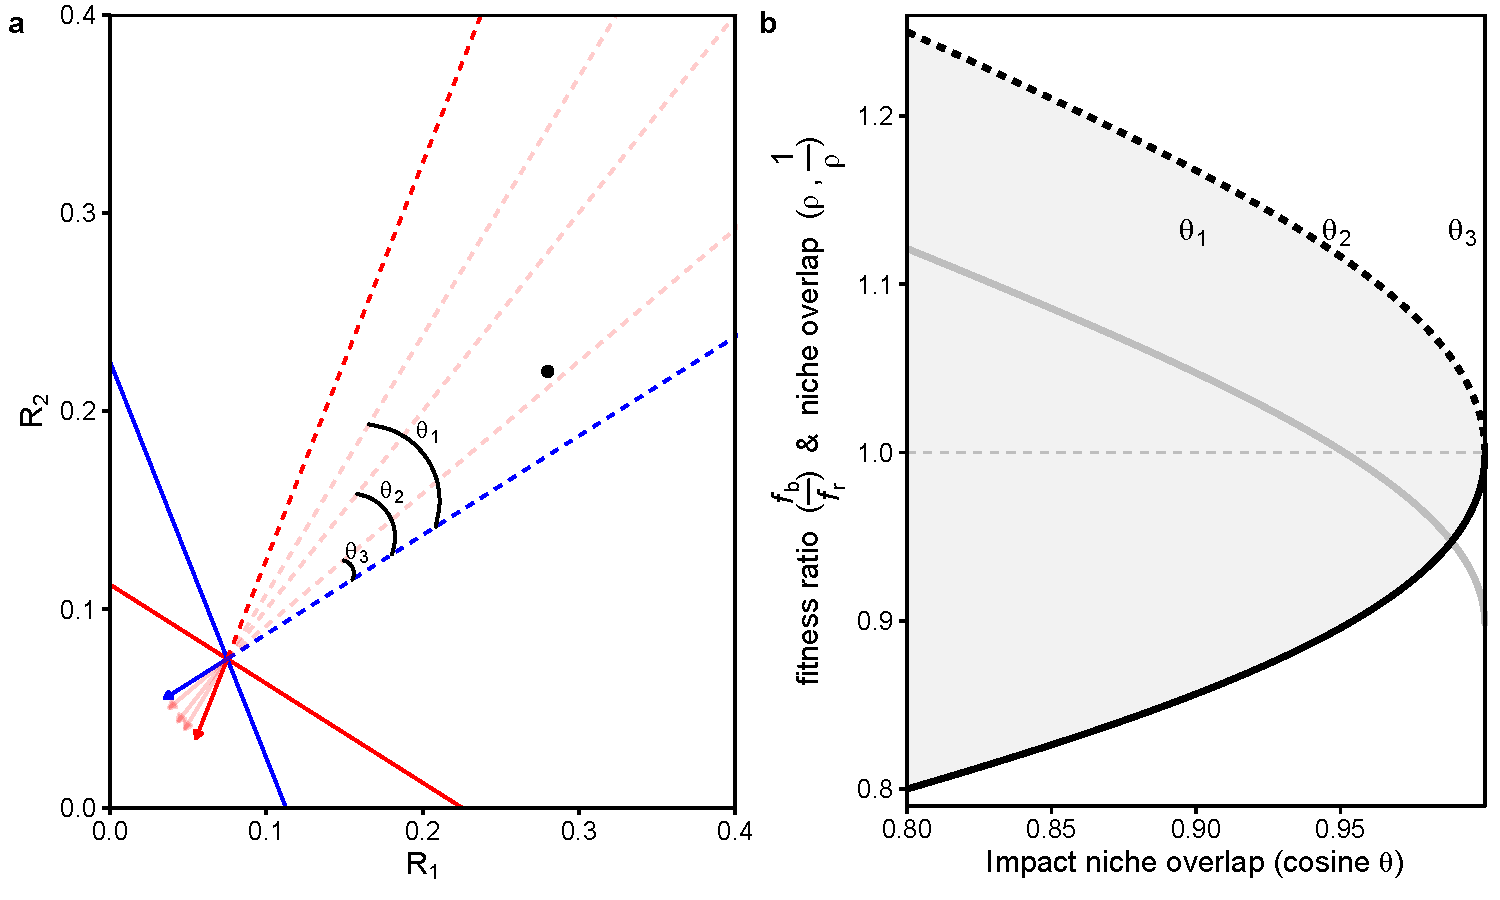
\includegraphics[width=12cm]{Chapter2/impact-appendix-fig-asymmetry-update.pdf}}
	\caption[The effect of changing impact niche overlap asymmetrically under pairwise competition for substitutable resources.]
		{\hspace{1mm}The effect of changing impact niche overlap asymmetrically under pairwise competition for substitutable resources. In (a), the solid red and blue lines are the ZNGIs for each species; the solid lines with arrow heads are the respective impact vectors; and the dashed lines are the inverse of the impact vectors, defining regions of stable coexistence. In (b), the x-axis represents the impact niche overlap starting from the position given by the solid bold impact vectors in (a) and ending at complete overlap. The y-axis gives the values of the fitness differences term, $f_{b}/f_{r}$ (solid grey line), and the degree of niche overlap, $\rho$ (solid black line) and $1/\rho$ (dashed black line). The grey shaded area indicates the coexistence region, where $\rho<f_{b}/f_{r}<1/\rho$. For reference, equal fitness, where $f_{b}/f_{r}=1$, is illustrated by the horizontal dashed grey line. The angles given by $\theta_{1-3}$ in (a) correspond to the respective $\theta_{1-3}$ in (b).}
	\label{fig:impact-appendix-fig-asymmetry}
\end{figure}



\clearpage
\section{Appendix S4}
Here, we show the effect on Chesson's niche overlap and fitness differences of rotating the impact vectors in a common direction whilst holding impact niche overlap constant. Note that the non-monotonic change in Chesson's niche overlap is an artifact of non-linearities in converting angular change into vectors. Because we used trigonometric functions (sine and cosine) to obtain new coordinates for the impact vectors while rotating them, the conversion from angles to coordinates was necessarily non-linear. More specifically, the rate of increase in the sine function decreases in the direction from 0 to 90 degrees, while the rate of decrease in the cosine function increases in the direction from 0 to 90 degrees. The implication of this is that although the angle defining impact niche overlap is held constant, there is a slight decoupling in the rates of change of the vector coordinates that are used in the mechanistic definition of Chesson's niche overlap term. This decoupling means that the rate at which the two species change in their impacts is not identical, which in turn translates into a spurious change in Chesson's niche overlap.  
\par


\newpage
\begin{figure}[H]
	\centering
	\makebox[\textwidth][c]{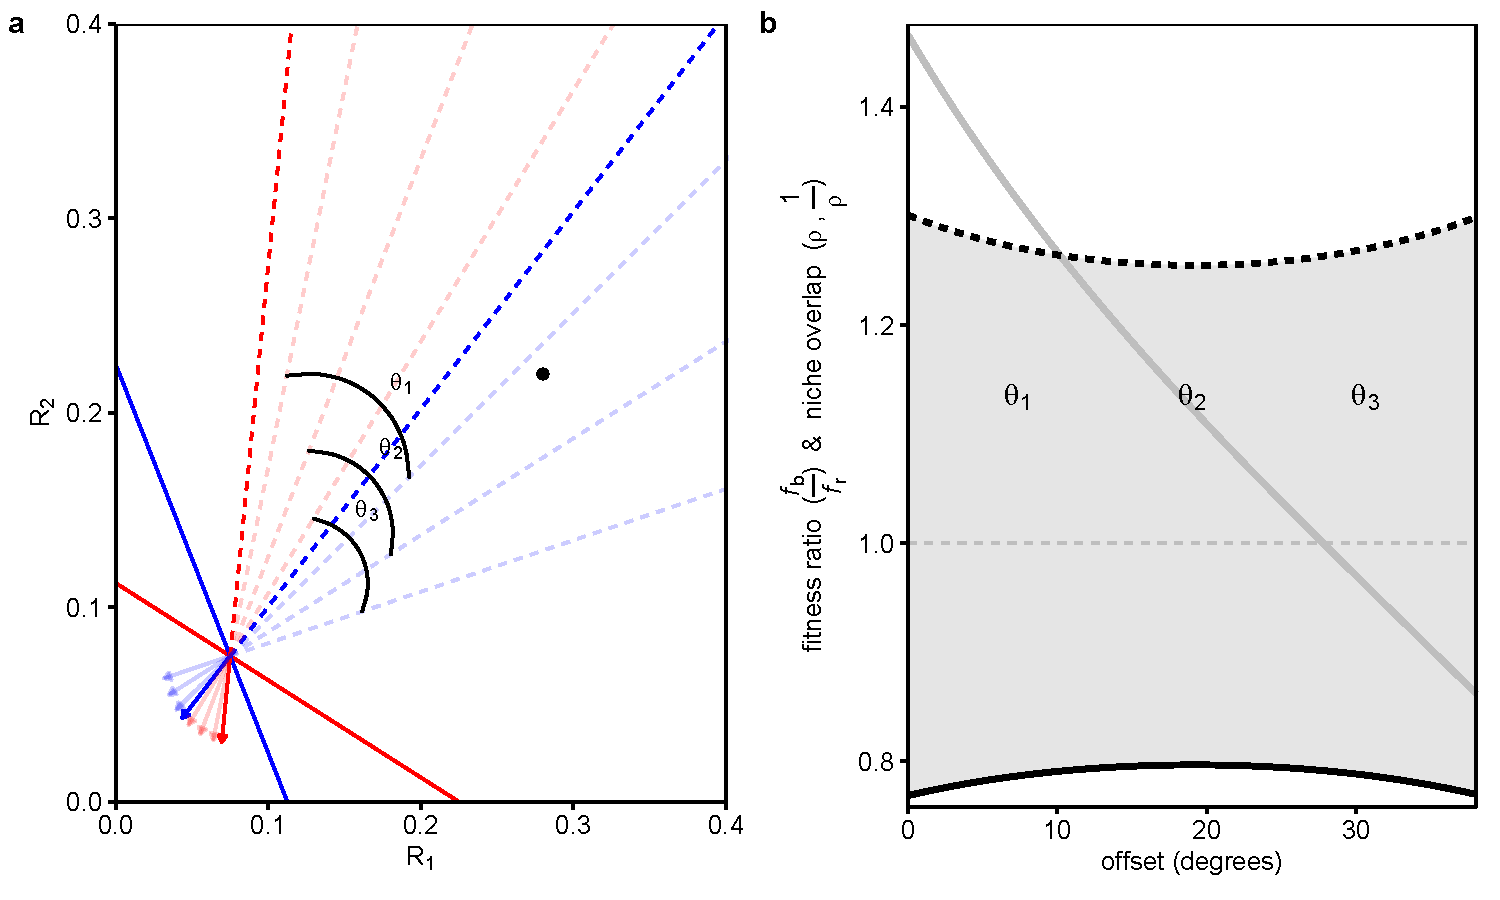
\includegraphics[width=12cm]{Chapter2/impact-ms-fig-fixed-overlap-appendix.pdf}}
	\caption[The effect of rotating the impact vectors in a common direction whilst holding impact niche overlap constant, under pairwise competition for substitutable resources.]
		{\hspace{1mm}The effect of rotating the impact vectors in a common direction whilst holding impact niche overlap constant, under pairwise competition for substitutable resources. In (a), the solid red and blue lines are the ZNGIs for each species; the solid lines with arrow heads are the respective impact vectors; and the dashed lines are the inverse of the impact vectors, defining regions of stable coexistence. In (b), the x-axis represents degrees that the impact vectors are rotated through starting from the position given by the solid bold impact vectors in (a). The y-axis gives the values of the fitness differences term, $f_{b}/f_{r}$ (solid grey line), and the degree of niche overlap, $\rho$ (solid black line) and $1/\rho$ (dashed black line). The grey shaded area indicates the coexistence region, where $\rho<f_{b}/f_{r}<1/\rho$. For reference, equal fitness, where $f_{b}/f_{r}=1$, is illustrated by the horizontal dashed grey line. The angles given by $\theta_{1-3}$ in (a) correspond to the respective $\theta_{1-3}$ in (b).}
	\label{fig:impact-appendix-fig-fix}
\end{figure}



\clearpage
\section{Appendix S5}
Here, we show the effect on Chesson's niche overlap and fitness difference of changing ZNGIs without fixing the resource equilibrium under competition for essential resources.
\par


\begin{figure}[H]
	\centering
	\makebox[\textwidth][c]{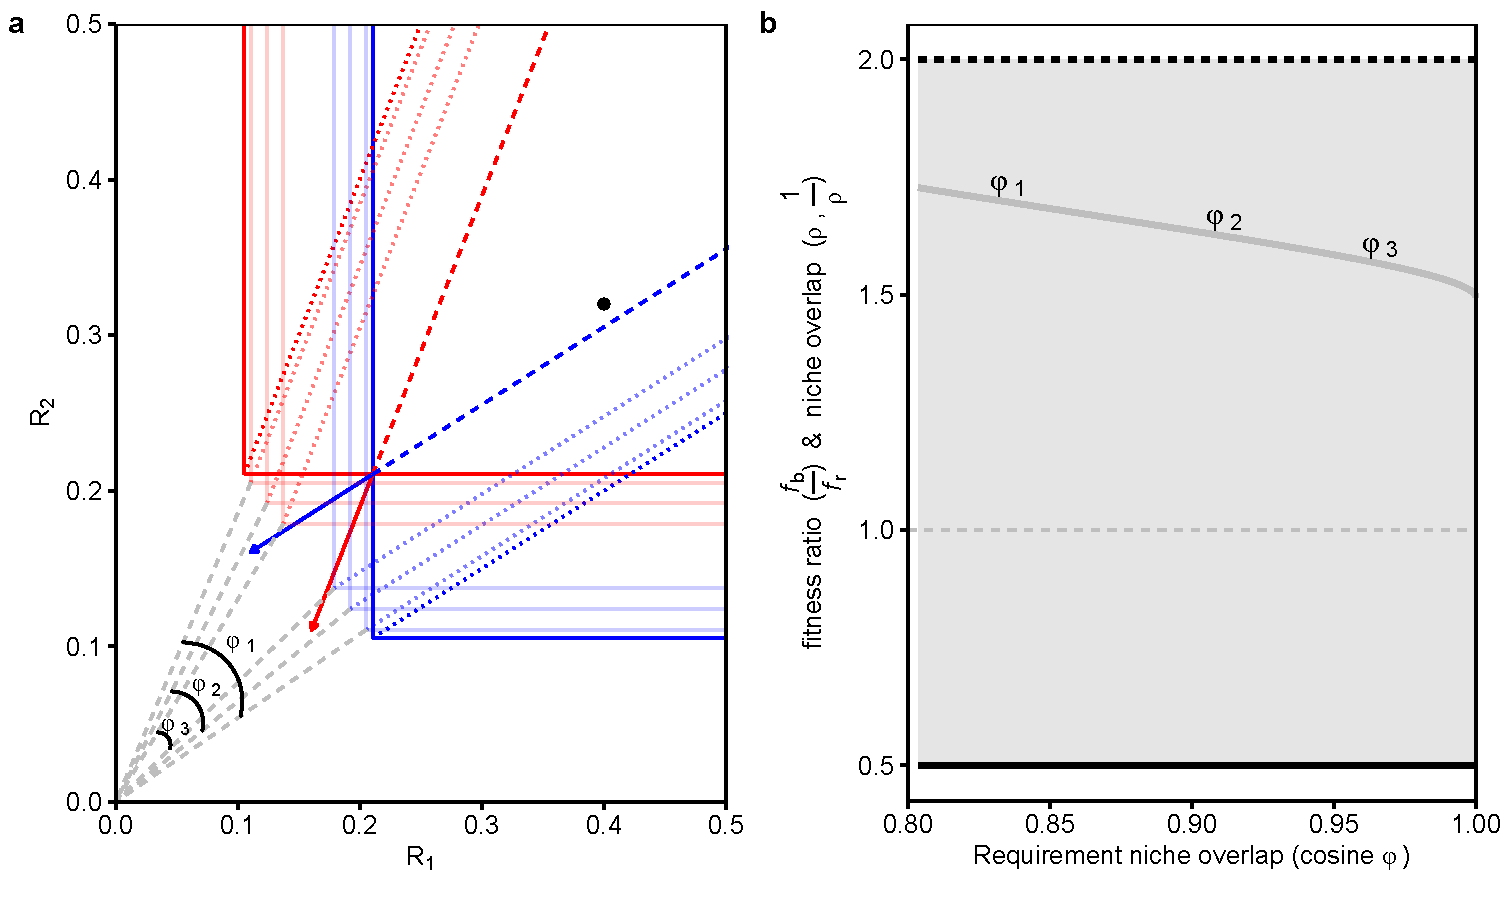
\includegraphics[width=12cm]{Chapter2/require-ms-fig-unfixedequilibrium-appendix.pdf}}
	\caption[The effects of changing requirement niche overlap without fixing the equilibrium resource density for the essential resources model.]
		{\hspace{1mm}The effects of changing requirement niche overlap without fixing the equilibrium resource density for the essential resources model. In (a), the solid red and blue lines are the ZNGIs for each species; the solid lines with arrow heads are the respective impact vectors; and the dashed lines are the inverse of the impact vectors, defining regions of stable coexistence. The additional dotted lines denote the regions in which species switch from being limited by different resources (above blue and below red) to being limited by the same resource (below blue or above red). In (b), the x-axis represents the requirement niche overlap starting from the position given by the solid bold ZNGIs in (a) and ending at complete overlap. The y-axis gives the values of the fitness differences term, $f_{b}/f_{r}$ (solid grey line), and the degree of niche overlap, $\rho$ (solid black line) and $1/\rho$ (dashed black line). The grey shaded area indicates the coexistence region, where $\rho<f_{b}/f_{r}<1/\rho$. For reference, equal fitness, where $f_{b}/f_{r}=1$, is illustrated by the horizontal dashed grey line. The angles given by $\varphi_{1-3}$ in (a) correspond to the respective $\varphi_{1-3}$ in (b).}
	\label{fig:require-appendix-fig-notfix}
\end{figure}


\chapter{Coexistence theory and the frequency-dependence of priority effects: Appendix S1}
%\chaptermark{Positive frequency-dependence}
%\renewcommand{\sectionmark}[1]{}
\fancyhead[LE, RO]{\thepage}
\fancyhead[RE]{APPENDIX B}
\fancyhead[LO]{POSITIVE FREQUENCY-DEPENDENCE}
\fancyfoot{}
\renewcommand{\headrulewidth}{0pt}
\setlength{\parindent}{1cm}


\begin{comment}
\documentclass[hidelinks,12pt]{article}
\usepackage{graphicx,bm, booktabs,lineno,array}
\usepackage[fleqn]{amsmath}
\setlength{\mathindent}{0pt}
\usepackage[super,comma,numbers, compress]{natbib}
\usepackage[a4paper]{geometry}
\usepackage[parfill]{parskip}
\usepackage[usenames,dvipsnames]{color}
\usepackage[font=footnotesize,labelfont=bf,margin=1cm, labelsep = none]{caption} 
\usepackage{setspace}
\usepackage{gensymb}
\usepackage{color} 
\usepackage{sidecap}
\usepackage{epigraph}
\usepackage{float}
\usepackage{soul,xcolor}
\setstcolor{red}
\setlength\epigraphwidth{12cm}
\setlength\epigraphrule{0pt}
\usepackage{etoolbox}
\usepackage{tcolorbox}
\tcbuselibrary{breakable}
\usepackage[bottom, symbol]{footmisc}
\usepackage{authblk}
\usepackage{hyperref}
\usepackage[color=cyan]{todonotes}
\pdfminorversion=3
\doublespacing

\renewcommand{\epigraphflush}{center}
\renewcommand{\sourceflush}{flushleft}
\newcommand{\plus}{\raisebox{.4\height}{\scalebox{.6}{+}}}
\newcommand{\minus}{\raisebox{.4\height}{\scalebox{.8}{-}}}
\renewcommand{\thefootnote}{\fnsymbol{footnote}}
\newcommand*\samethanks[1][\value{footnote}]{\footnotemark[#1]}
\newcommand\blfootnote[1]{%
\begingroup
\renewcommand\thefootnote{}\footnote{#1}%
\addtocounter{footnote}{-1}%
\endgroup
}
\end{comment}



\begin{comment}
\title{Coexistence theory and the frequency-dependence of priority effects}
\author[1]{Po-Ju Ke \thanks{Both authors contributed equally.}}
\author[1,2,3]{Andrew D. Letten \samethanks}
\affil[1]{Department of Biology, Stanford University, Stanford, California, 94305-5020, USA}
\affil[2]{Centre for Integrative Ecology, University of Canterbury, Christchurch, New Zealand}
\affil[3]{Institute of Integrative Biology, Department of Environmental Systems Science, ETH Z{\"u}rich, 8092 Z{\"u}rich, Switzerland}

\begin{document}

\date{}
\maketitle
\blfootnote{Correspondence email: pojuke@stanford.edu, andrew.letten@usys.ethz.ch}
%\textbf{Running title:} PFD
%\textbf{Keywords:} No key words for Forum 
\textbf{Type of article:} Brief Communication\\
\textbf{Number of words:} 1847 [main text] \\
\textbf{References:} 17\\
\textbf{Display items:} 3\\
\end{comment}



\section{Appendix S1 -- Positive frequency dependence in an equilibrium and nonequilibrium systems}
\subsection*{Positive frequency dependence in an equilibrium system}
In Figure~\ref{fig:Fig1} in the main text we provided an example of PFD emerging from resource competition in an equilibrium system. To produce Figure~\ref{fig:Fig1} we used the approach implemented in Letten \textit{et al.} (2017) \citep{Letten2017} to translate changes in the parameters of Tilman's consumer-resource model \citep{tilman1982} into changes to the stabilization potential and fitness ratio of coexistence theory (but see \citep{Meszenaz2006} and \cite{Kleinhesselink2015} for an alternative approach). In this part of the supplementary methods we explain the underlying mathematical treatment. 
\par


The key to the approach in \citep{Letten2017} is to solve the coexistence equilibrium of a consumer resource model and rearrange it algebraically to a form that is comparable to the equilibrium of a two species Lotka--Volterra competition model. To better understand the procedure, consider a Lotka--Volterra competition model for two consumer species (i.e., $N_{1}$ and $N_{2}$):

\begin{equation}
\frac{dN_{1}}{dt}=r_{1}N_{1}\left ( 1-a_{11}N_{1}-a_{12}N_{2} \right )
\tag{S3.1.1}\label{eq:S3.1.1}
\end{equation}
\begin{equation}
\frac{dN_{2}}{dt}=r_{2}N_{2}\left ( 1-a_{21}N_{1}-a_{22}N_{2} \right ). 
\tag{S3.1.2}\label{eq:S3.1.2}
\end{equation}

\noindent This simple model has two monoculture fixed point of either species, i.e., $N_{i} = \frac{1}{\alpha_{ii}}$, as well as a coexistence fixed point that simultaneously fulfills  $N_{1}^{*}=\frac{1}{a_{11}}-\frac{a_{12}}{a_{11}}N_{2}^{*}$ and $N_{2}^{*}=\frac{1}{a_{22}}-\frac{a_{21}}{a_{22}}N_{1}^{*}$. In panel c of Fig.~\ref{fig:FigBox}, we demonstrate that the coexistence fixed point is the only stable equilibrium with the following parameters: $r_{1} = r_{2} = 0.1$, $\alpha_{12} = 0.96$, $\alpha_{21} = 0.8$, and $\alpha_{11} = \alpha_{22} = 1.4$. In panel a of Fig.~\ref{fig:FigBox}, alternative stable states, such that the competition outcome is one of the two monoculture fixed point depending on species' initial density, can emerge when $\alpha_{11} = \alpha_{22} = 0.64$. To demonstrate alternative stable states, we started trajectories from either higher density of $N_{1}$ (upper panels: $N_{1(0)}=1$, $N_{2(0)}=0.2$) or $N_{2}$ (lower panels: $N_{1(0)}=0.2$, $N_{2(0)}=1$). 
\par


For Figure~\ref{fig:Fig1}, we take Tilman's model \citep[p.~270]{tilman1982} where two consumers (i.e., $N_{1}$ and $N_{2}$) are competing for two perfectly substitutable resources, $R_{1}$ and $R_{2}$, and solve for its coexistence equilibrium. The dynamics of this system can be described as follows:

\begin{equation}
\frac{{d{N_1}}}{{dt}} = {r_1}{N_1}\left[ {\frac{{{w_{11}}{R_1} + {w_{12}}{R_2} - {T_1}}}{{{k_1} + {w_{11}}{R_1} + {w_{12}}{R_2} - {T_1}}}} \right] - D{N_1}
\tag{S3.2.1}\label{eq:S3.2.1}
\end{equation}
\begin{equation}
\frac{{d{N_2}}}{{dt}} = {r_2}{N_2}\left[ {\frac{{{w_{21}}{R_1} + {w_{22}}{R_2} - {T_2}}}{{{k_2} + {w_{21}}{R_1} + {w_{22}}{R_2} - {T_2}}}} \right] - D{N_2}
\tag{S3.2.2}\label{eq:S3.2.2}
\end{equation}
\begin{equation}
\frac{{d{R_1}}}{{dt}} = D\left( {{S_1} - {R_1}} \right) - {c_{11}}{N_1} - {c_{21}}{N_2}
\tag{S3.2.3}\label{eq:S3.2.3}
\end{equation}
\begin{equation}
\frac{{d{R_2}}}{{dt}} = D\left( {{S_2} - {R_2}} \right) - {c_{12}}{N_1} - {c_{22}}{N_2}.
\tag{S3.2.4}\label{eq:S3.2.4}
\end{equation}

\noindent Here, $r_{i}$ represents the maximum population growth rate for species $i$ ($i = $ 1 or 2) and $D$ represents the constant mortality of the consumers and turnover rate of resources. Per capita resource consumption rate of consumer $N_{i}$ on resource $R_{j}$ ($j = $ 1 or 2) is represented by $c_{ij}$, whereas $w_{ij}$ represents a weighting factor that converts availability of $R_{j}$ into its value for consumer $N_{i}$. Following a Monod growth model, $k_{i}$ is the half-saturation constant for $N_{i}$ resource consumption, and $T_{i}$ is the minimum amount of total resource required for $N_{i}$ to grow. Finally, $S_{1}$ and $S_{2}$ represent the resource supply concentrations for $R_{1}$ and $R_{2}$, respectively. Certain assumptions of this Monod growth model, such as constant supply of resource and strong recipient control of consumption rate, may not be applicable to many systems. However, this should not affect the results qualitatively \cite{Kleinhesselink2015}. 
\par


Following the same mathematical trick in Appendix A.1, we can transform Eqns.~\ref{eq:S3.2.1} -- \ref{eq:S3.2.4} to a Lotka--Volterra form and derive Eqns.~\ref{eq:3.11} and \ref{eq:3.12}. In Figure~\ref{fig:Fig1}, we plotted the ZNGI, the consumption vectors (species 1 in red and species 2 in blue), and the supply point (see Appendix A.1 for definition). The consumption vectors for consumer $i$ on the two substitutable resources is a vector with elements $\left( c_{i1}, c_{i2} \right)$, and the supply point can be expressed as a point with coordinates $\left( S_{1}, S_{2} \right)$. To study the effects of changing consumer resource parameters on stabilization potential (defined as 1 - $\rho$ in the main text) and fitness ratio, we varied species' per capita consumption rates, $c_{ij}$, and the supply point. To keep the position of the ZNGIs fixed, we set the following parameters as: $D = 0.7$, $k_{1} = k_{2} = 0.4$, $r_{1} = r_{2} = 1$, $T_{1} = T_{2} = 0.1$, $w_{11} = w_{22} = 2$, and $w_{12} = w_{21} = 4$. 
\par


In panel (a) and (b), each species consumes more of its favored resource but with different degree of resource partitioning. The per capita consumption rates in panel (a) are $c_{11} = c_{22} = 2$ and $c_{21} = c_{12} = 4$, whereas that in panel (b) are $c_{11} = c_{22} = 2.843$ and $c_{21} = c_{12} = 3.452$. In panel (c) and (d), each species now consumes more of the resource favored by its competitor with $c_{11} = c_{22} = 3.552$ and $c_{21} = c_{12} = 2.718$. This potentially leads to priority effects depending on the fitness ratio between the two species, which can be altered by modifying the supply point from the black circle $\left(0.3, 0.38\right)$ to the black square $\left(0.248, 0.245 \right)$. 
\par


\subsection*{Positive frequency dependence in an non-equilibrium system}
In Figure~\ref{fig:Fig2} in the main text we provide an example of PFD emerging through the coexistence-affecting mechanism relative non-linearity. In this example two consumers compete for a single logistically-growing resource. One species has a type 3 functional response (blue in Fig.~\ref{fig:Fig2}), given by: 

\begin{equation}
\frac{dN_{1}}{dt} = N_{1}(\mu _{max_{1}}\frac{R^2}{Ks_{1} + R^2}-d).
\tag{S3.3.1}\label{eq:S3.3.1}
\end{equation}

\noindent The other species (red in Fig.~\ref{fig:Fig2}) has a modified Monod (type 2) functional response with inhibition at high resource levels: 

\begin{equation}
\frac{dN_{2}}{dt} = N_{2}(\mu _{max_{2}}\frac{R}{Ks_{2} + R + \frac{R^2}{Ki}}-d).
\tag{S3.3.2}\label{eq:S3.3.2}
\end{equation}

\noindent Here, $N_{i}$ is the population density of consumer $i$ ($i = $ 1 or 2), $\mu_{max_{i}}$ is the maximum growth rate, $Ks_{i}$ is the half saturation constant, $R$ is the density/concentration of resource, $d$ is the density independent mortality rate, and $Ki$ is the inhibition term unique to the second species. 
\par


\noindent Resource dynamics are given by:

\begin{equation}
\frac{dR}{dt} = rR(1-\frac{R}{K}) - \sum_{i = 1}^{n} Q_{i}\frac{\mathrm{d}N_{i}}{\mathrm{d}t},\qquad i = 1,2, 
\tag{S3.3.3}\label{eq:S3.3.3}
\end{equation}

\noindent where $r$ is the resource intrinsic rate of increase, $K$ is the resource carrying capacity and $Q_{i}$ is the resource quota of consumer $i$. 
\par


We used the following values for the parameters in Figure~\ref{fig:Fig2}: $\mu_{max_{1}} = 0.029$, $\mu_{max_{2}} = 0.2$, $Ks_{1} = 0.02$, $Ks_{2} = 3$, $d = 0.01$, $Ki = 1$, $r = 0.5$, $K = 3$, $Q_{1} = 0.01$ and $Q_{2} = 0.01$. Simulations were run with the LSODA solver using the deSolve package v1.20 \citep{soetaert2016package} in R v3.4.2. In Fig.~\ref{fig:Fig2}b, the simulation was started with starting population sizes of 500 and 1 for blue and red respectively. In Fig.~\ref{fig:Fig2}c, the simulation was started with starting population sizes of 1 and 500 for blue and red respectively. 


\chapter{Effects of soil microbes on plant competition: a perspective from modern coexistence theory: Appendices S1 -- S4}
%\chaptermark{Positive frequency-dependence}
%\renewcommand{\sectionmark}[1]{}
\fancyhead[LE, RO]{\thepage}
\fancyhead[RE]{APPENDIX C}
\fancyhead[LO]{SOIL MICROBES AND PLANT COEXISTENCE}
\fancyfoot{}
\renewcommand{\headrulewidth}{0pt}
\setlength{\parindent}{1cm}


\begin{comment}
\documentclass[hidelinks,12pt]{article}
\usepackage{graphicx,bm, booktabs,lineno,array}
\usepackage[fleqn]{amsmath}
\setlength{\mathindent}{0pt}
\usepackage[super,comma,numbers, compress]{natbib}
\usepackage[a4paper]{geometry}
\usepackage[parfill]{parskip}
\usepackage[usenames,dvipsnames]{color}
\usepackage[font=footnotesize,labelfont=bf,margin=1cm, labelsep = none]{caption} 
\usepackage{setspace}
\usepackage{gensymb}
\usepackage{color} 
\usepackage{sidecap}
\usepackage{epigraph}
\usepackage{float}
\usepackage{soul,xcolor}
\setstcolor{red}
\setlength\epigraphwidth{12cm}
\setlength\epigraphrule{0pt}
\usepackage{etoolbox}
\usepackage{tcolorbox}
\tcbuselibrary{breakable}
\usepackage[bottom, symbol]{footmisc}
\usepackage{authblk}
\usepackage{hyperref}
\usepackage[color=cyan]{todonotes}
\pdfminorversion=3
\doublespacing

\renewcommand{\epigraphflush}{center}
\renewcommand{\sourceflush}{flushleft}
\newcommand{\plus}{\raisebox{.4\height}{\scalebox{.6}{+}}}
\newcommand{\minus}{\raisebox{.4\height}{\scalebox{.8}{-}}}
\renewcommand{\thefootnote}{\fnsymbol{footnote}}
\newcommand*\samethanks[1][\value{footnote}]{\footnotemark[#1]}
\newcommand\blfootnote[1]{%
\begingroup
\renewcommand\thefootnote{}\footnote{#1}%
\addtocounter{footnote}{-1}%
\endgroup
}
\end{comment}



\begin{comment}
\begin{document}

\doublespacing
\title{Effects of soil microbes on plant competition: \\ a perspective from modern coexistence theory}
\author[* 1]{Po-Ju Ke}
\author[* 1, 2]{Joe Wan}
\affil[1]{Department of Biology, Stanford University, Stanford, California 94305-5020, USA}
\affil[2]{Institute of Integrative Biology, Department of Environmental Systems Science, ETH Z\"{u}rich, 8092 Z\"{u}rich, Switzerland}
\date{}
\maketitle
\blfootnote{* Both authors contributed equally}
\blfootnote{Correspondence author: Department of Biology, Stanford University, Stanford, California 94305-5020, USA. Phone: +1 650-721-1711. Email: pojuke@stanford.edu, jwan@student.ethz.ch}

\onehalfspacing
\noindent \textbf{Type of article:} Concepts and Synthesis\\
\noindent \textbf{Running head:} Soil microbes and plant coexistence\\
% \noindent \textbf{Keywords:} fitness difference, mutualism, niche difference, pathogens, plant--soil feedback\\
% \begin{myindentpar}{1cm}
	\textbf{Words in Abstract:} 233\\
	\textbf{Words in main text:} 7658\\
	% \textbf{Words in text boxes:} 241\\
	\textbf{Number of references:} 65\\
	\textbf{Number of figures:} 5\\
	\textbf{Number of tables:} 1\\
	\textbf{Number of text boxes:} 2\\
% \end{myindentpar}

% \noindent \textbf{Authorship statement:} PJK conceived the study; PJK and JW performed the analysis and wrote the manuscript.\\

% \noindent \textbf{Data accessibility statement:} No original data appear in this manuscript. Should the manuscript be accepted, all computer scripts supporting the results will be archived in an appropriate public repository such as Github, with the DOI included at the end of the article.\\

\doublespacing
\linenumbers
\end{comment}



\section{Appendix S1 -- Deriving the general plant--soil microbe interaction model from other candidate models}
To illustrate how modern coexistence theory can be applied to study plant-soil microbe interactions, in the main text we used \citet{Eppinga2006} as an example model. While we demonstrated how this model can be converted to a phenomenological Lotka-Volterra form, it is not the only modeling possibility -- under some circumstances other models may be more suitable. Here, we briefly show how our approach can be applied to two other potential models, which cover a wide range of dynamics between plants and their associated soil microbial community.
\par


\subsubsection*{Resource uptake as the process governing plant--plant competition}
We consider a model that explicitly captures resource competition as the mechanism behind plant--plant competition. The full three-trophic level model closely follows the model in \citet{Chesson2008b}. The density of soil resources are represented by $R_{l}$ ($l=1$ or $2$), whereas the density of plants and soil microbes are represented by $N_{i}$ and $S_{i}$ ($i=A$ or $B$), respectively. The dynamics of the three-trophic level model is captured by the following dynamic system:

\begin{equation}
%\frac{dR_{i}}{dt} = r_{i}^{R} R_{i} \left ( 1 - \frac{R_{i} }{K_{i}^{R}} \right ) - a_{iA}R_{i}N_{A}  - a_{iB}R_{i}N_{B}
\frac{dR_{l}}{dt} = r_{l}^{R} R_{l} \left ( 1 - \frac{R_{l} }{K_{l}^{R}} \right ) - a_{lA}R_{l}N_{A}  - a_{lB}R_{l}N_{B}
\tag{S4.1}\label{eq:Resource_RCmodel}
\end{equation}
\begin{equation}
%\frac{dN_{i}}{dt} = e_{Ai}a_{Ai}R_{A}N_{i}  + e_{Bi}a_{Bi}R_{B}N_{i} + \left( \sigma_{iA}S_{A}+\sigma_{iB}S_{B} \right)N_{i} - d_{i}N_{i}
\frac{dN_{i}}{dt} = e_{1i}a_{1i}R_{1}N_{i}  + e_{2i}a_{2i}R_{2}N_{i} + \left( \sigma_{iA}S_{A}+\sigma_{iB}S_{B} \right)N_{i} - d_{i}N_{i}
\tag{S4.2}\label{eq:Plant_RCmodel}
\end{equation}
\begin{equation}
\frac{dS_{i}}{dt } = g_{i}S_{i}\left ( 1-\frac{S_{i}}{k_{i}}\right ) .
\tag{S4.3}\label{eq:Soil_RCmodel}
\end{equation}

\noindent Here, resources follow logistic growth, with intrinsic growth rate and carrying capacity $r_{l}^{R}$ and $K_{l}^{R}$, respectively. The superscript $R$ indicates that these parameters are associated with resource dynamics. Plants compete with each other via consuming, and thus lowering the amount of available, resources: $R_{l}$ is consumed by plant species $N_{A}$ and $N_{B}$ with consumption rates $a_{lA}$ and $a_{lB}$, respectively. The two resources $R_{1}$ and $R_{2}$ are assumed to be substitutable, and contribute to plant population size $N_{i}$ after being assimilated, with conversion efficiency, $e_{1i}$ and $e_{2i}$, respectively. Plants die with density-independent morality rate, $d_{i}$. Finally, soil dynamics are assumed to follow the same dynamics as Eqns.~\ref{eq:SoilA} and \ref{eq:SoilB} in the main text. Under the assumption of logistically growing resources, this model can also be simplified to a Lotka-Volterra form after applying separation of timescales (i.e., assuming both resources and soil microbes are the fast variable).
In particular, the quasi-equilibrium for resources are $\hat{R_{l}}= K_{l}^{R} - \frac{K_{l}^{R}}{r_{l}^{R}} \left ( a_{lA}N_{A}+a_{lB}N_{B} \right )$, whereas that for soil microbes are $\hat{S_{i}}= \phi_{i} \times N_{i}$. Substituting these expressions into Eqn.~\ref{eq:Plant_RCmodel}:

\makeatletter
\def\tagform@#1{\maketag@@@{\normalsize(#1)\@@italiccorr}}
\makeatother
\footnotesize
\begin{equation}
\begin{split}
\frac{dN_{A}}{dt}\frac{1}{N_{A}}& = \left ( e_{1A}a_{1A}K_{1}^{R} + e_{2A}a_{2A}K_{2}^{R} - d_{A} \right ) \times \\
& \quad \left [ 1 +
\left ( -\frac{ K_{1}^{R}}{r_{1}^{R}}e_{1A}a_{1A}^{2} - \frac{K_{2}^{R}}{r_{2}^{R}}e_{2A}a_{2A}^{2} + \sigma_{AA}\phi_{A} \right )\frac{N_{A}}{r_{A}}
+ \left ( -\frac{ K_{1}^{R}}{r_{1}^{R}}e_{1A}a_{1A}a_{1B} - \frac{K_{2}^{R}}{r_{2}^{R}}e_{2A}a_{2A}a_{2B} + \sigma_{AB}\phi_{B} \right )\frac{N_{B}}{r_{A}} \right ]
\end{split}
\tag{S4.4}\label{eq:LVA_RCmodel}
\end{equation}
\begin{equation}
\begin{split}
\frac{dN_{B}}{dt}\frac{1}{N_{B}}& = \left ( e_{1B}a_{1B}K_{1}^{R} + e_{2B}a_{2B}K_{2}^{R} - d_{B} \right ) \times \\
& \quad \left [ 1 +
\left ( -\frac{ K_{1}^{R}}{r_{1}^{R}}e_{1B}a_{1B}a_{1A} - \frac{K_{2}^{R}}{r_{2}^{R}}e_{2B}a_{2B}a_{2A} + \sigma_{BA}\phi_{A} \right )\frac{N_{A}}{r_{B}}
+ \left ( -\frac{ K_{1}^{R}}{r_{1}^{R}}e_{1B}a_{1B}^{2} - \frac{K_{2}^{R}}{r_{2}^{R}}e_{2B}a_{2B}^{2} + \sigma_{BB}\phi_{B} \right )\frac{N_{B}}{r_{B}} \right ]
\end{split}
\tag{S4.5}\label{eq:LVB_RCmodel}
\end{equation}
\normalsize

\noindent where $r_{i} = e_{1i}a_{1i}K_{1}^{R} + e_{2i}a_{2i}K_{2}^{R} - d_{i}$. The interaction coefficient among competing plants, $\alpha_{ij}$, can be written as:

\begin{equation}
\alpha_{ij} =
\left ( \frac{-\frac{ K_{1}^{R}}{r_{1}^{R}}e_{1i}a_{1i}a_{1j} - \frac{K_{2}^{R}}{r_{2}^{R}}e_{2i}a_{2i}a_{2j}}
{e_{1i}a_{1i}K_{1}^{R} + e_{2i}a_{2i}K_{2}^{R} - d_{i}}\right )
+ \left ( \frac{\sigma_{ij}\phi_{j}}
{e_{1i}a_{1i}K_{1}^{R} + e_{2i}a_{2i}K_{2}^{R} - d_{i}}\right ).
\tag{S4.6}\label{eq:alpha_RCmodel}
\end{equation}

\noindent The above expression takes the same form as Eqn.~\ref{eq:alpha} in the main text, and thus can be thought as a mechanistic decomposition of Eqn.~\ref{eq:alpha}. In particular, the term enclosed in the first parenthesis represents plant--plant competition whereas the second parenthesis represents plant--soil microbe interactions. Note that since we are modeling plant--plant competition via resource uptake, the first term in Eqn.~\ref{eq:alpha_RCmodel} would always be negative (i.e., negative $c_{ij}$ in the main text).
With this expression of $\alpha_{ij}$, one can then calculate the niche overlap and fitness ratio between $N_{A}$ and $N_{B}$ using the equations provided in \citet{Chesson1990, Chesson2008b}.
\par


\subsubsection*{Soil microbes are conditioned by both plant species}
In our modified \citet{Eppinga2006} model, soil microbial community $S_{i}$ exhibits strong host specificity and is only conditioned by plant $N_{i}$. In some systems, soil microbes might be more generalists and are conditioned by both plant species (i.e., $N_{i}$ conditions not only $S_{i}$ but also $S_{j}$). In this model, we assume a host-specificity conditioning ratio, $h_{i}$, for each plant species: $N_{i}$ allocates proportion $h_{i}$ of its conditioning ability, $\phi_{i}$ to soil microbial community $S_{i}$ and proportion $\left(1-h_{i}\right)$ to $S_{j}$. The dynamics of this dynamic sysem can be represented as follows:

\begin{equation}
%\frac{dN_{i}}{dt} = r_{i}N_{i} \left( 1 + \frac{c_{ii}N_{i}+c_{ij}N_{j}}{K_{i}} \right) + \left( \sigma_{ii}'S_{i}+\sigma_{ij}'S_{j} \right)N_{i}
\frac{dN_{i}}{dt} = r_{i}N_{i} \left( 1 + c_{ii}N_{i}+c_{ij}N_{j} + \sigma_{ii}'S_{i}+\sigma_{ij}'S_{j} \right)N_{i}
\tag{S4.7}\label{eq:Plant_Cocondition}
\end{equation}
\begin{equation}
\frac{dS_{i}}{dt } = g_{i}S_{i}\left ( 1-\frac{S_{i}}{k_{i}}\right ) .
\tag{S4.8}\label{eq:Soil_Cocondition}
\end{equation}

\noindent In this model, both $N_{i}$ and $N_{j}$ condition soil microbial community $S_{i}$, and the microbial community affects plant performance with interaction coefficient $\sigma_{ij}'$. The carrying capacity of soil microbes, $k_{i}$, is:

\begin{equation}
%k_{i}=h_{i}\frac{N_{i}}{K_{i}}\phi_{i} + \left ( 1-h_{j} \right )\frac{N_{j}}{K_{j}}\phi_{j}.
k_{i} = h_{i}\phi_{i}N_{i} + \left ( 1-h_{j} \right )\phi_{j}N_{j} .
\tag{S4.9}\label{eq:SoilCarrying_Cocondition}
\end{equation}

\noindent By applying the separation of timescales with the assumption that soil microbes are the fast variable compared to plants, we obtain the following Lotka-Volterra:

\makeatletter
\def\tagform@#1{\maketag@@@{\normalsize(#1)\@@italiccorr}}
\makeatother
\footnotesize
\begin{equation}
\frac{dN_{A}}{dt}\frac{1}{N_{A}} = r_{A} \left [ 1 +
\left ( c_{AA} + \sigma_{AA}'h_{A}\phi_{A} + \sigma_{AB}'\left ( 1-h_{A} \right )\phi_{A} \right )N_{A} + \left ( c_{AB} + \sigma_{AB}'h_{B}\phi_{B} + \sigma_{AA}'\left ( 1-h_{B} \right ) \phi_{B} \right )N_{B} \right ]
\tag{S4.10}\label{eq:LVA_Cocondition}
\end{equation}
\begin{equation}
\frac{dN_{B}}{dt}\frac{1}{N_{B}} = r_{B} \left [ 1 +
\left ( c_{BA} + \sigma_{BA}'h_{A}\phi_{A} + \sigma_{BB}'\left ( 1-h_{A} \right ) \phi_{A} \right )N_{A} + \left ( c_{BB} + \sigma_{BB}'h_{B}\phi_{B} + \sigma_{BA}'\left ( 1-h_{B} \right )\phi_{B} \right )N_{B} \right ]
\tag{S4.11}\label{eq:LVB_Cocondition}
\end{equation}
\normalsize

\noindent With the above equation, one then derive the intra- and inter-specific plant--plant interaction coefficients, $\alpha_{ii}$ and $\alpha_{ij}$, as follows:

\begin{equation}
\alpha_{ii} = c_{ii} + \left [ \sigma_{ii}'h_{i} + \sigma_{ij}'\left ( 1-h_{i} \right ) \right ]\phi_{i}
\tag{S4.12}\label{eq:alpha_Cocondition_con}
\end{equation}
\begin{equation}
\alpha_{ij} = c_{ij} + \left [ \sigma_{ij}'h_{j} + \sigma_{ii}'\left ( 1-h_{j} \right ) \right ]\phi_{j} .
\tag{S4.13}\label{eq:alpha_Cocondition_heter}
\end{equation}

\noindent The above expression takes the same form as Eqn.~\ref{eq:alpha} in the main text, with $\sigma_{ij}$ being partitioned into effects coming from two different soil microbial communities (i.e., the $\sigma_{ij}'$ and $\sigma_{ii}'$ terms enclosed in the bracket).
As one can observe, this model reduces to our modified \citet{Eppinga2006} model when plants only condition their associated soil microbes (i.e., $h_{i}=h_{j}=1$). An alternative way to interpret this new expression is that our original $\sigma_{ij}$ (Eqn.~\ref{eq:alpha}) is a phenomenological summary of its separated components. Again, with this expression of $\alpha_{ij}$, one can then calculate the niche overlap and fitness ratio between $N_{A}$ and $N_{B}$.
\par



\section{Appendix S2 -- Separating stabilizing and equalizing components}
To calculate the components of modern coexistence theory, we applied separation of timescales to reduce the dimensions of our model (Eqns. \ref{eq:SoilA}-\ref{eq:Nb}) to a Lotka--Volterra, an approach that was also used in many classic studies \citep{MacArthur1970, Chesson1990}. In particular, we assumed that the dynamics of soil microbes are sufficiently fast (the fast variable) compared to that of the plants (the slow variable) and all dynamics occur near the equilibrium. These assumptions allowed us to calculate the quasi-equilibrium of the two soil communities, $\hat{S_{i}}$, by setting Eqns.~\ref{eq:SoilA} and \ref{eq:SoilB} in the main text as zero and assuming the slow variables are unchanging:

\begin{equation}
%\hat{S_{i}}= k_{i}= \frac{N_{i}}{K_{i}}\times \phi_{i}
\hat{S_{i}}= k_{i}= N_{i} \times \phi_{i}
\tag{S4.14} \label{eq:QuasiSoil}
\end{equation}

\noindent where $i = A$ or $B$. To understand the dynamics of the slow variable, we substituted this quasi-equilibrium into Eqns.~\ref{eq:Na} and \ref{eq:Nb} by assuming the soil communities always remain near their quasi-equilibrium:

\begin{equation}
\frac{dN_{A}}{dt } = r_{A}N_{A}\left [1 + \left(c_{AA}+\sigma_{AA}\phi_{A}\right)N_{A} + \left(c_{AB}+\sigma_{AB}\phi_{B}\right)N_{B}\right ]
\tag{S4.15}\label{eq:NaLV}
\end{equation}
\begin{equation}
\frac{dN_{B}}{dt } = r_{B}N_{B}\left [1 + \left(c_{BA}+\sigma_{BA}\phi_{A}\right)N_{A} + \left(c_{BB}+\sigma_{BB}\phi_{B}\right)N_{B}\right ] .
\tag{S4.16}\label{eq:NbLV}
\end{equation}

\noindent The resulting simplified model is a two species Lotka--Volterra model, with species' per capita growth rate as a linear function of intra- and inter-specific densities.
The interaction coefficients, $\alpha_{ij}$, shown below in equation \ref{eq:S_alpha}, consist of both plant--plant competition that are not related to soil microbes, $c_{ij}$, and soil microbial effects, summarized as $\sigma_{ij}\phi_{j}$.
We assumed plant--plant interactions are competitive ($c_{ij} < 0$) whereas plant--soil microbe interactions can be either detrimental ($\sigma_{ij} < 0$) or beneficial ($\sigma_{ij} > 0$). Our model simplifies to the classic Lotka--Volterra competition model when $\sigma_{ij}$ or $\phi_{i} = 0$:

\begin{equation}
\alpha_{ij} = c_{ij} + \sigma_{ij}\phi_{j} .
\tag{S4.17}\label{eq:S_alpha}
\end{equation}

\noindent After transforming the model into a Lotka--Volterra form, we can now quantify niche overlap and fitness ratio among the two plants \citep{Chesson1990, Chesson2008b, Chesson2013ecosys}. Note that the following analytical definition of these terms were derived specifically for a two-species Lotka--Volterra framework. Thus, it ignores other coexistence mechanisms that rely on temporal fluctuation and spatial variation (but see \cite{Chesson2003, Barabas2018} for a more generalizable definition of these components). With this formalization, stabilizing mechanisms represent processes that decrease niche overlap, $\rho$ (or increases niche difference, $1-\rho$). Here, $\rho$ is defined as a symmetric measure of the ratio of inter- to intra-specific density dependence based on Lotka--Volterra coefficients, i.e., $\rho = \sqrt{\frac{\alpha_{BA}\alpha_{AB}}{\alpha_{AA}\alpha_{BB}}}$. Accordingly, we derived the niche overlap between $N_{A}$ and $N_{B}$ as:

\begin{equation}
\rho = \sqrt{\frac{\left ( c_{BA} + \sigma_{BA}\phi_{A} \right )
						   \left ( c_{AB} + \sigma_{AB}\phi_{B} \right )}
						  {\left ( c_{AA} + \sigma_{AA}\phi_{A} \right )
						   \left ( c_{BB} + \sigma_{BB}\phi_{B} \right )}} .
\tag{S4.18}\label{eq:S_ND}
\end{equation}

\noindent Equalizing mechanisms, on the other hand, represent processes that reduce the fitness ratio between species, which is defined as $\frac{f_{B}}{f_{A}} = \sqrt{\frac{\alpha_{AA}\alpha_{AB}}{\alpha_{BB}\alpha_{BA}}}$. According, we derived this term for our model as:

\begin{equation}
\frac{f_{B}}{f_{A}} = \sqrt{\frac{\left ( c_{AA} + \sigma_{AA}\phi_{A} \right )
											    \left ( c_{AB} + \sigma_{AB}\phi_{B} \right )}
											   {\left ( c_{BB} + \sigma_{BB}\phi_{B} \right )
												\left ( c_{BA} + \sigma_{BA}\phi_{A} \right )}} .
\tag{S4.19}\label{eq:S_FR}
\end{equation}
\par



\section{Appendix S3 -- Invasion analysis for the plant--soil microbe interaction model}
Here, we perform invasion analysis and demonstrate how it aids understanding for our results. This is done by assuming that one of the two species (the invader) is at low density while the other (the resident) is at its mono-dominance equilibrium, such that the invader is affected by the resident but itself has no effects on its surroundings. Under such scenario, the per capita growth rate of the resident is zero and that for the invader is called its invasion growth rate (IGR). If both species, when as the invader, have positive invasion growth rates, they can stably coexist as both are able to recover from low density. To see how this works, let us first consider a two-species Lotka--Volterra competition model:

\begin{equation}
\frac{dN_{A}}{dt} = r_{A}N_{A}\left ( 1-\alpha_{AA}N_{A}-\alpha_{AB}N_{B} \right )
\tag{S4.20}\label{eq:S_LVA}
\end{equation}
\begin{equation}
\frac{dN_{B}}{dt} = r_{B}N_{B}\left ( 1-\alpha_{BA}N_{A}-\alpha_{BB}N_{B} \right ) .
\tag{S4.21}\label{eq:S_LVB}
\end{equation}

\noindent First, assume $N_{A}$ is at invader state and $N_{B}$ is at its mono-dominance equilibrium, $\frac{1}{\alpha_{BB}}$, which is obtained by setting equation \ref{eq:S_LVB} to zero under $N_{A}$ equal zero. The invasion growth rate of $N_{A}$, $IGR_{A}$ is derived as:

\begin{equation}
IGR_{A} =
\left.\begin{matrix}
\frac{1}{N_{A}}\frac{dN_{A}}{dt}
\end{matrix}\right|
_{N_{A}=0, N_{B}=\frac{1}{\alpha_{BB}}} = r_{A}\left( 1 - \frac{\alpha_{AB}}{\alpha_{BB}}\right) .
\tag{S4.22}\label{eq:S_IGR_A}
\end{equation}

\noindent If $IGR_{A}$ is greater than zero, then $N_{A}$ can recover from arbitrarily low density, preventing itself from being excluded. As mentioned, it is important to observe that the sign of $IGR_{A}$ depends solely on the intra- and inter-specific interaction coefficients of $N_{B}$ ($\alpha_{BB}$ and $\alpha_{AB}$, respectively). This makes sense: $N_{A}$, as the invader, is too rare to have any impact on the surroundings and thus its growth rate is only determined by the impact from the resident species. The same process applies when $N_{B}$ is the invader and $N_{A}$ is at its mono-dominance equilibrium, $\frac{1}{\alpha_{AA}}$. Note that while this method can be generalized to $n-$species community, careful thought needs to be given when considering the coexistence of all the combinations of remaining $n-1$ species \citep{Barabas2018}. For two species simple Lotka--Volterra there is no problem since if one species goes extinct, the other one will always persist.
\par


Now, we can perform invasion analysis for our simplified plant--soil interaction model (Eqns.~\ref{eq:NaLV} and \ref{eq:NbLV}), which takes the form of a simple two-species Lotka--Volterra model as shown in Eqns.~\ref{eq:S_LVA} and \ref{eq:S_LVB}. The invasion growth rate will thus take the same form as Eqn \ref{eq:S_IGR_A}, with $\alpha_{ij}$ following \ref{eq:S_alpha}:

\begin{equation}
IGR_{A} =
r_{A}\left [ 1 - \left ( \frac{c_{AB}+\sigma_{AB}\phi_{B}} {c_{BB}+\sigma_{BB}\phi_{B}} \right ) \right ]
\tag{S4.23}\label{eq:IGR_A}
\end{equation}
\begin{equation}
IGR_{B} =
r_{B}\left [ 1 - \left ( \frac{c_{BA}+\sigma_{BA}\phi_{A}} {c_{AA}+\sigma_{AA}\phi_{A}} \right ) \right ] .
\tag{S4.24}\label{eq:IGR_B}
\end{equation}
\par



\clearpage
\section{Appendix S4 -- Supplementary Tables and Figures}
\begin{table}[h]
	\centerfloat
	\caption[Default parameter values for each plant--soil microbe interaction scenario.]
	{Default parameter values for each plant--soil microbe interaction scenario (see main text for the detailed simulation process and the range of parameter variation for plant-mediated competition, $c_{ij}$).}
	\label{table:Parameters}
	\begin{tabular}{lcccc}
		\toprule \textbf{Parameter} & \textbf{Janzen-Connell} & \textbf{enemy release} & \textbf{mutual facilitation} & \textbf{soil conditioning} \tabularnewline
		\midrule
		\midrule
		$\phi_{A}$    &  1.6          &  0.5      &  0.15       &  0.025 \tabularnewline
		$\phi_{B}$    &  2.0          &  0.5      &  0.20       &  0.025 -- 2.5 \tabularnewline
		$\sigma_{AA}$ & -0.32 -- -6.0 & -0.5      &  0.5        &  0.50 \tabularnewline
		$\sigma_{AB}$ & -0.4          & -0.5      &  0.0 -- 2.0 &  0.25 \tabularnewline
		$\sigma_{BB}$ & -0.32 -- -6.0 & -2.0 -- 0 &  0.5        &  0.20 \tabularnewline
		$\sigma_{BA}$ & -0.5          & -2.0 -- 0 &  0.0 -- 2.0 &  0.10 \tabularnewline
		$c_{AA}$      & -1.0          & -1.5      & -1.0        & -1.0 \tabularnewline
		$c_{AB}$      & -1.0          & -1.0      & -1.0        & -1.0 \tabularnewline
		$c_{BB}$      & -0.8          & -1.5      & -1.0        & -0.9 \tabularnewline
		$c_{BA}$      & -0.8          & -1.0      & -1.0        & -0.9 \tabularnewline
		\bottomrule
	\end{tabular}%
\end{table}
\bigskip\bigskip\bigskip\bigskip
\bigskip\bigskip\bigskip\bigskip



\clearpage
\begin{figure}[htbp]
	\centering
	\makebox[\textwidth][c]{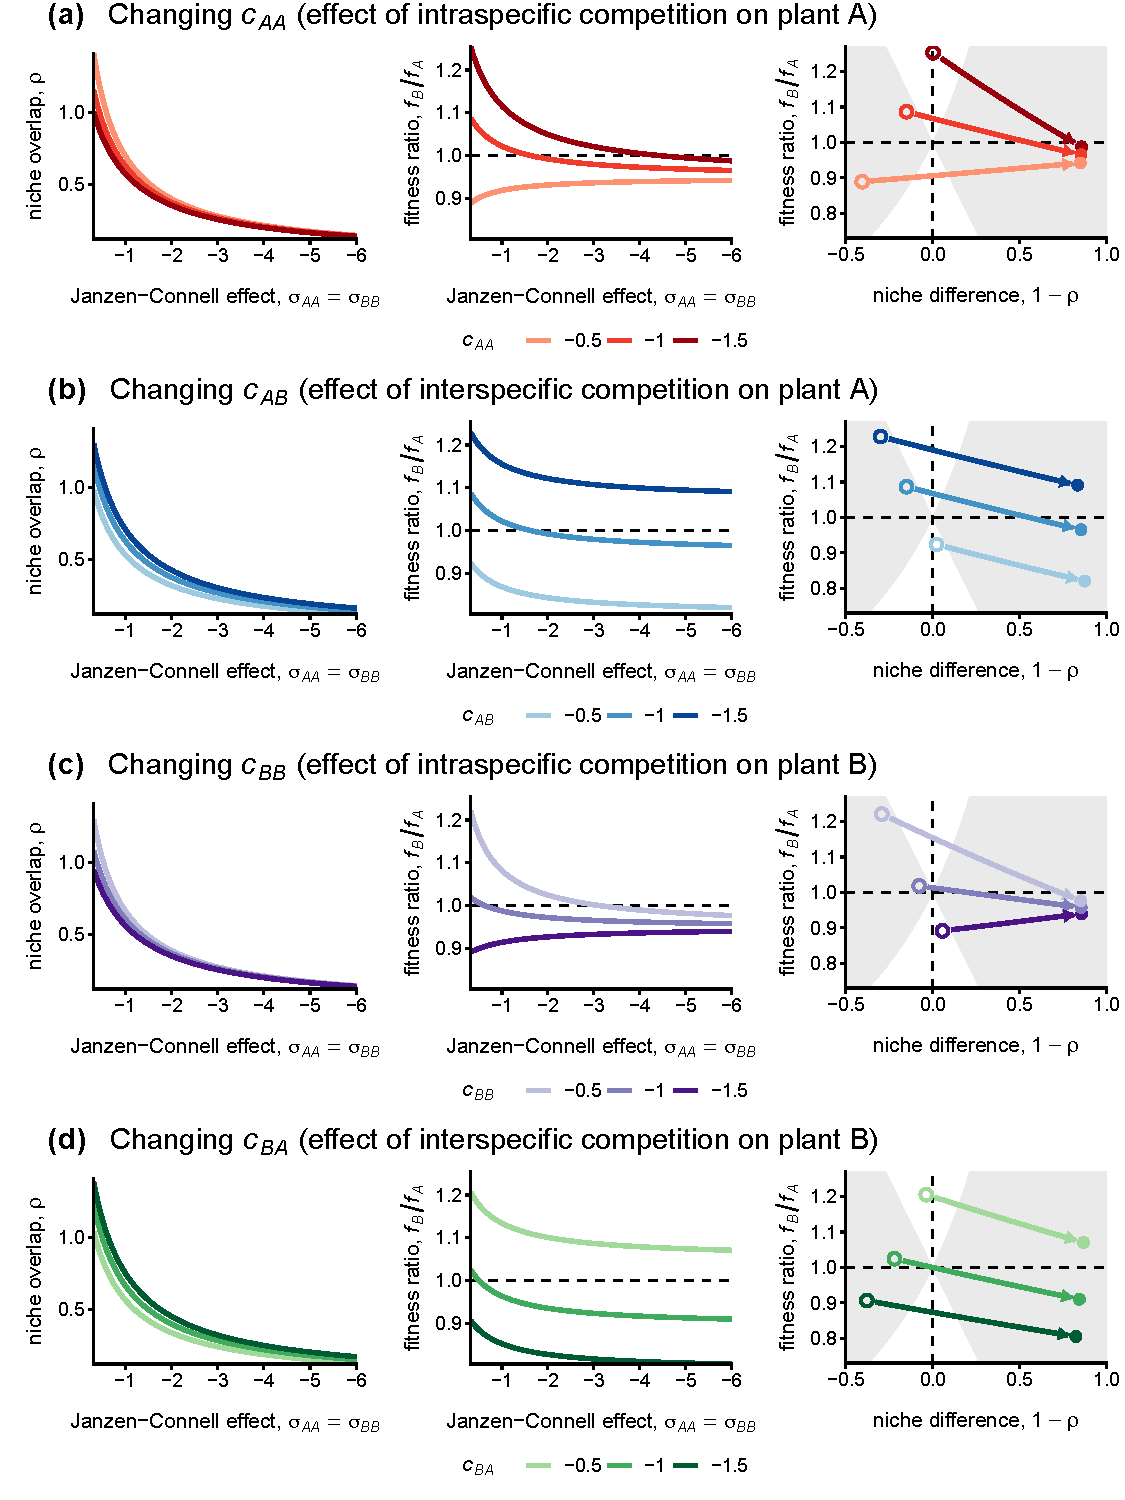
\includegraphics[width=12cm]{Chapter4/Translated_Janzen_Connell_full.pdf}}
	\caption[The effects of varying plant--soil microbe interactions ($\sigma_{AA}$ and $\sigma_{BB}$) and plant--plant competition on competitive outcomes for the Janzen--Connell scenario.]
		{The effects of varying plant--soil microbe interactions ($\sigma_{AA}$ and $\sigma_{BB}$) and plant--plant competition on competitive outcomes for the Janzen--Connell scenario.
		Each row (panel a--d) represent the effects of varying one plant--plant competition coefficient while keeping the other three constant: (a) $c_{AA}$, in red colors; (b) $c_{AB}$, in blue colors; (c) $c_{BB}$, in purple colors; (d) $c_{BA}$, in green colors. Lines with different brightness represent different plant--plant competition strength, ranging from weak (light colors) to strong (dark colors).
		The first two columns represent the effects of varying $\sigma_{AA}$ and $\sigma_{BB}$ on niche overlap ($\rho$) and fitness ratio ($f_{B}/f_{A}$), respectively. The third column visualizes the changes in the two components on the parameter space of niche difference ($1 - \rho$, x-axis) and fitness ratio ($f_{B}/f_{A}$, y-axis). Arrows represent the effects of changing plant--soil microbe interactions, from weakest (open circle) to strongest (solid circle). See also Fig.~\ref{fig:Scenario_Battleaxes} legend.} 
	\label{fig:Janzen_Connell_everything}
\end{figure}



\clearpage
\begin{figure}[htbp]
	\centering
	\makebox[\textwidth][c]{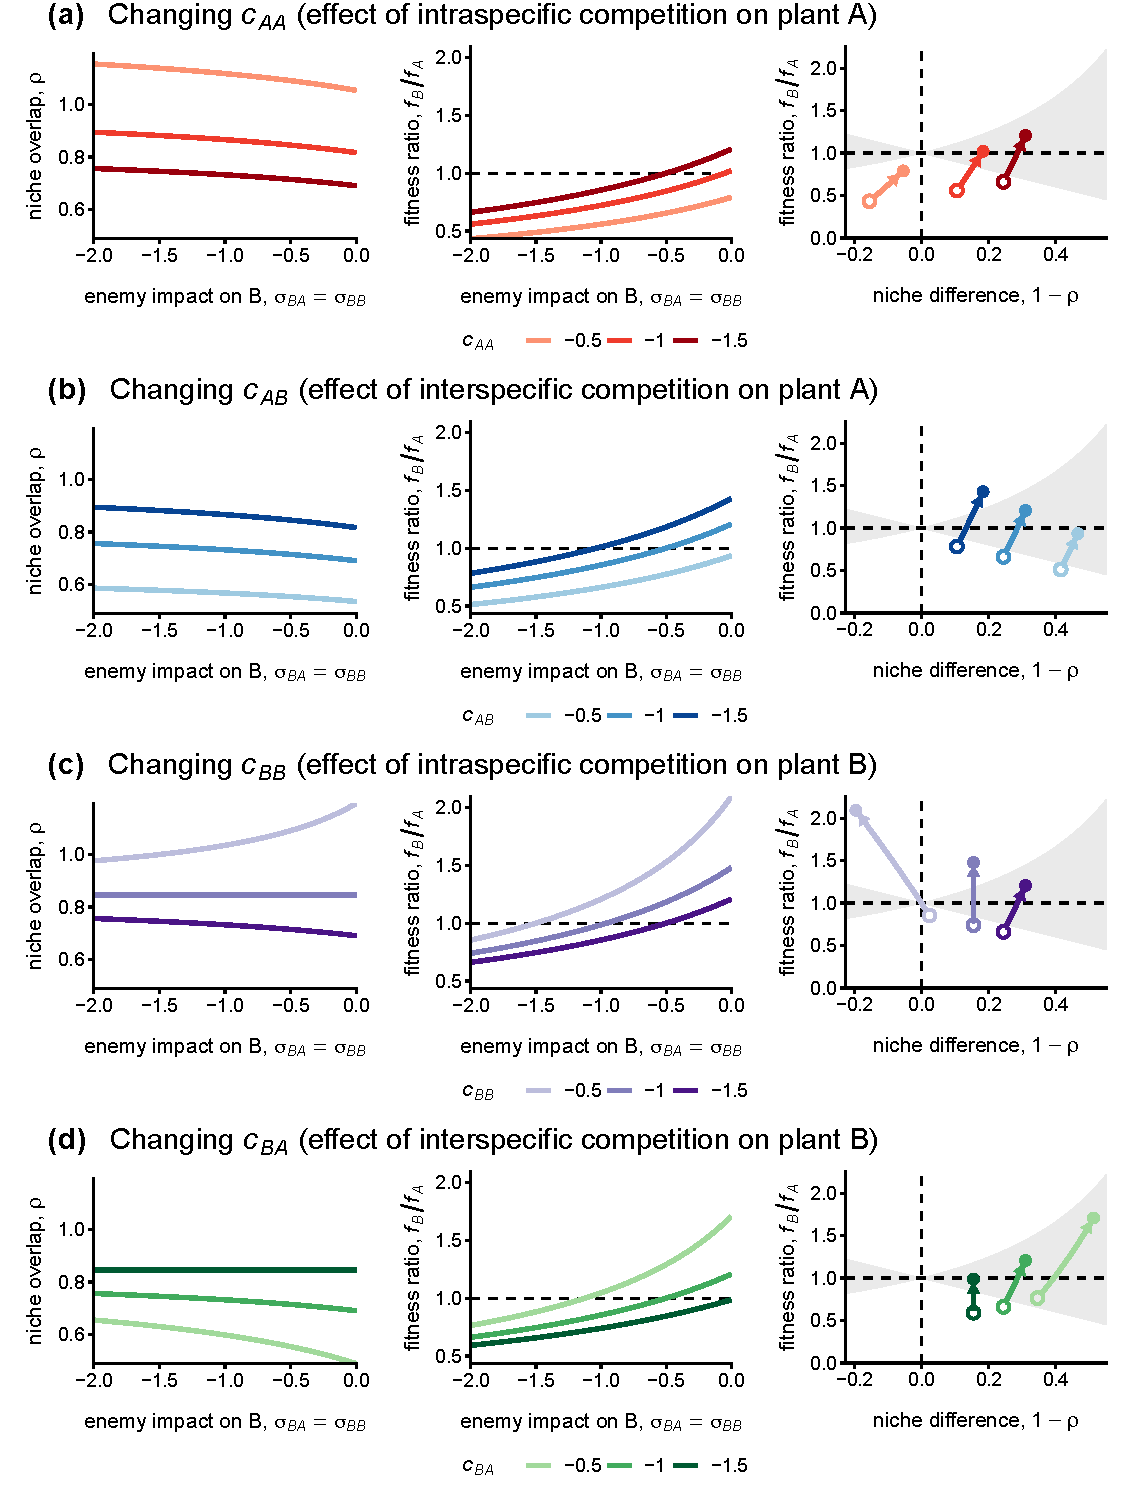
\includegraphics[width=12cm]{Chapter4/Translated_Enemy_Release_full.pdf}}
	\caption[The effects of varying plant--soil microbe interactions ($\sigma_{BA}$ and $\sigma_{BB}$) and plant--plant competition on competition outcomes for the enemy release scenario.]
		{The effects of varying plant--soil microbe interactions ($\sigma_{BA}$ and $\sigma_{BB}$) and plant--plant competition on competition outcomes for the enemy release scenario.
		Each row (panel a--d) represent the effects of varying one plant--plant competition coefficient while keeping the other three constant: (a) $c_{AA}$, in red colors; (b) $c_{AB}$, in blue colors; (c) $c_{BB}$, in purple colors; (d) $c_{BA}$, in green colors. Lines with different brightness represent different plant--plant competition strength, ranging from weak (light colors) to strong (dark colors).
		The first two columns represent the effects of varying $\sigma_{BA}$ and $\sigma_{BB}$ on niche overlap ($\rho$) and fitness ratio ($f_{B}/f_{A}$), respectively. The third column visualizes the changes in the two components on the parameter space of niche difference ($1 - \rho$, x-axis) and fitness ratio ($f_{B}/f_{A}$, y-axis). Arrows represent the effects of changing plant--soil microbe interactions, from weakest (open circle) to strongest (solid circle). See also Fig.~\ref{fig:Scenario_Battleaxes} legend.}
	\label{fig:Enemy_Release_everything}
\end{figure}



\clearpage
\begin{figure}[htbp]
	\centering
	\makebox[\textwidth][c]{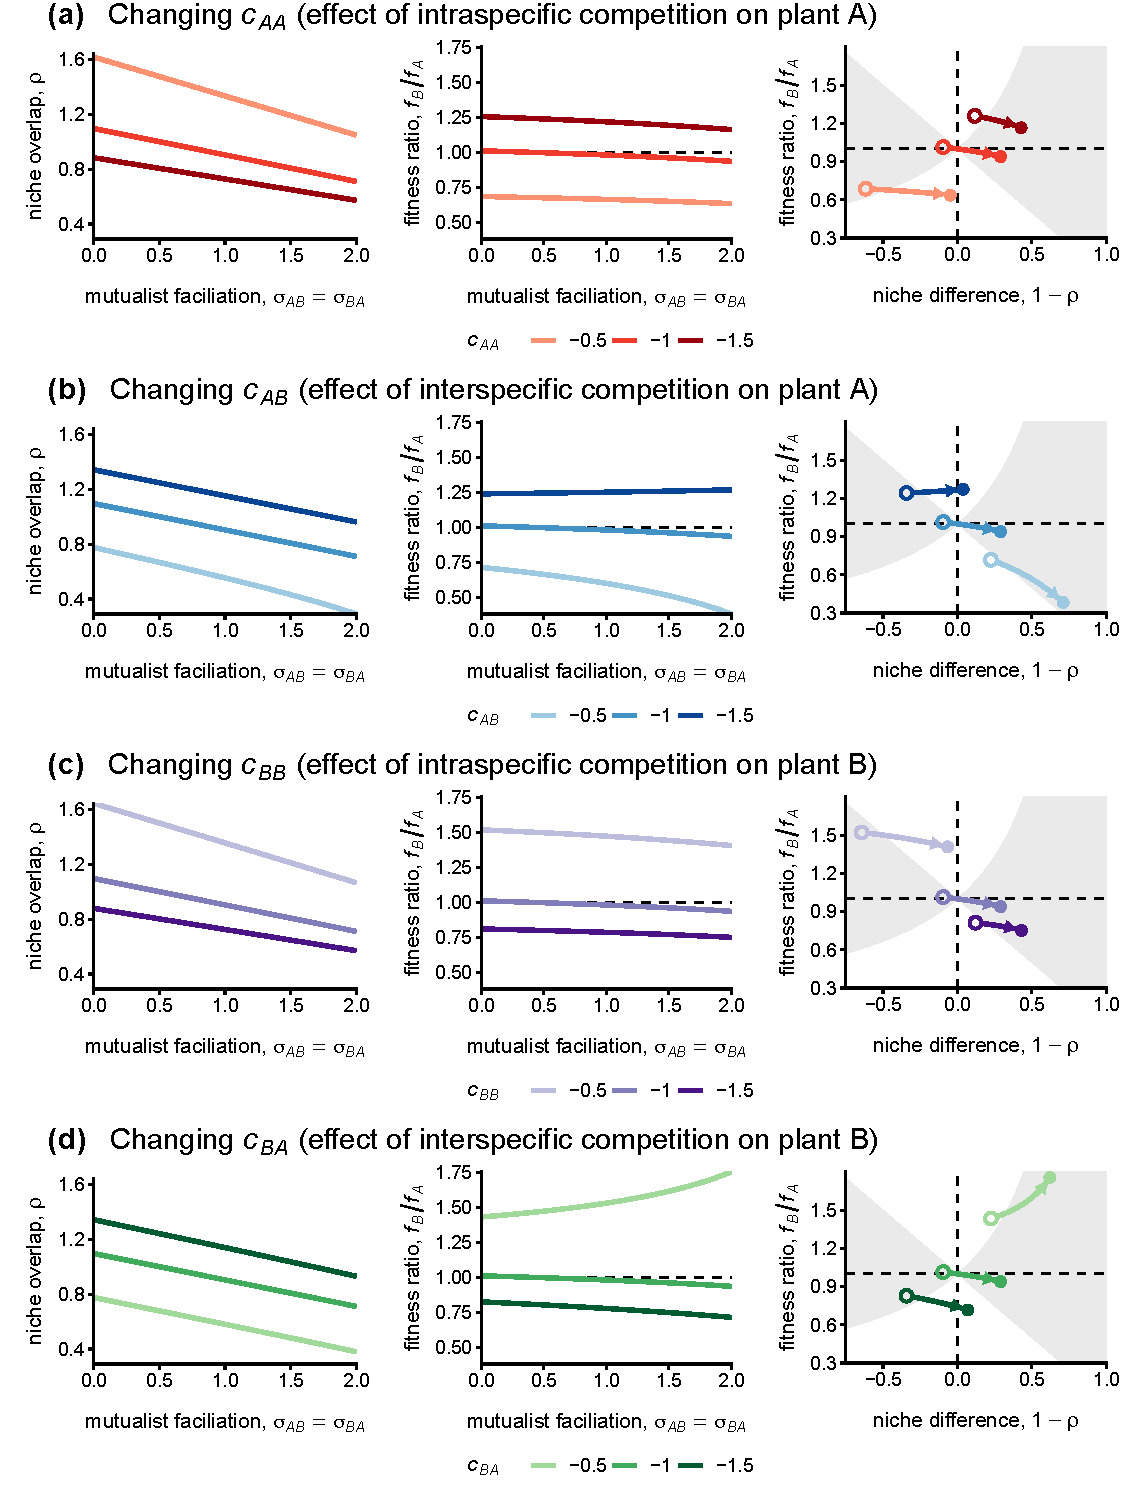
\includegraphics[width=12cm]{Chapter4/Translated_Mutual_Facilitation_full.pdf}}
	\caption[The effects of varying plant--soil microbe interactions ($\sigma_{BA}$ and $\sigma_{AB}$) and plant--plant competition on competition outcomes for the mutual facilitation scenario.]
		{The effects of varying plant--soil microbe interactions ($\sigma_{BA}$ and $\sigma_{AB}$) and plant--plant competition on competition outcomes for the mutual facilitation scenario.
		Each row (panel a--d) represent the effects of varying one plant--plant competition coefficient while keeping the other three constant: (a) $c_{AA}$, in red colors; (b) $c_{AB}$, in blue colors; (c) $c_{BB}$, in purple colors; (d) $c_{BA}$, in green colors. Lines with different brightness represent different plant--plant competition strength, ranging from weak (light colors) to strong (dark colors).
		The first two columns represent the effects of varying $\sigma_{BA}$ and $\sigma_{AB}$ on niche overlap ($\rho$) and fitness ratio ($f_{B}/f_{A}$), respectively. The third column visualizes the changes in the two components on the parameter space of niche difference ($1 - \rho$, x-axis) and fitness ratio ($f_{B}/f_{A}$, y-axis). Arrows represent the effects of changing plant--soil microbe interactions, from weakest (open circle) to strongest (solid circle). See also Fig.~\ref{fig:Scenario_Battleaxes} legend.}
	\label{fig:Mutual_Facilitation_everything}
\end{figure}



\clearpage
\begin{figure}[htbp]
	\centering
	\makebox[\textwidth][c]{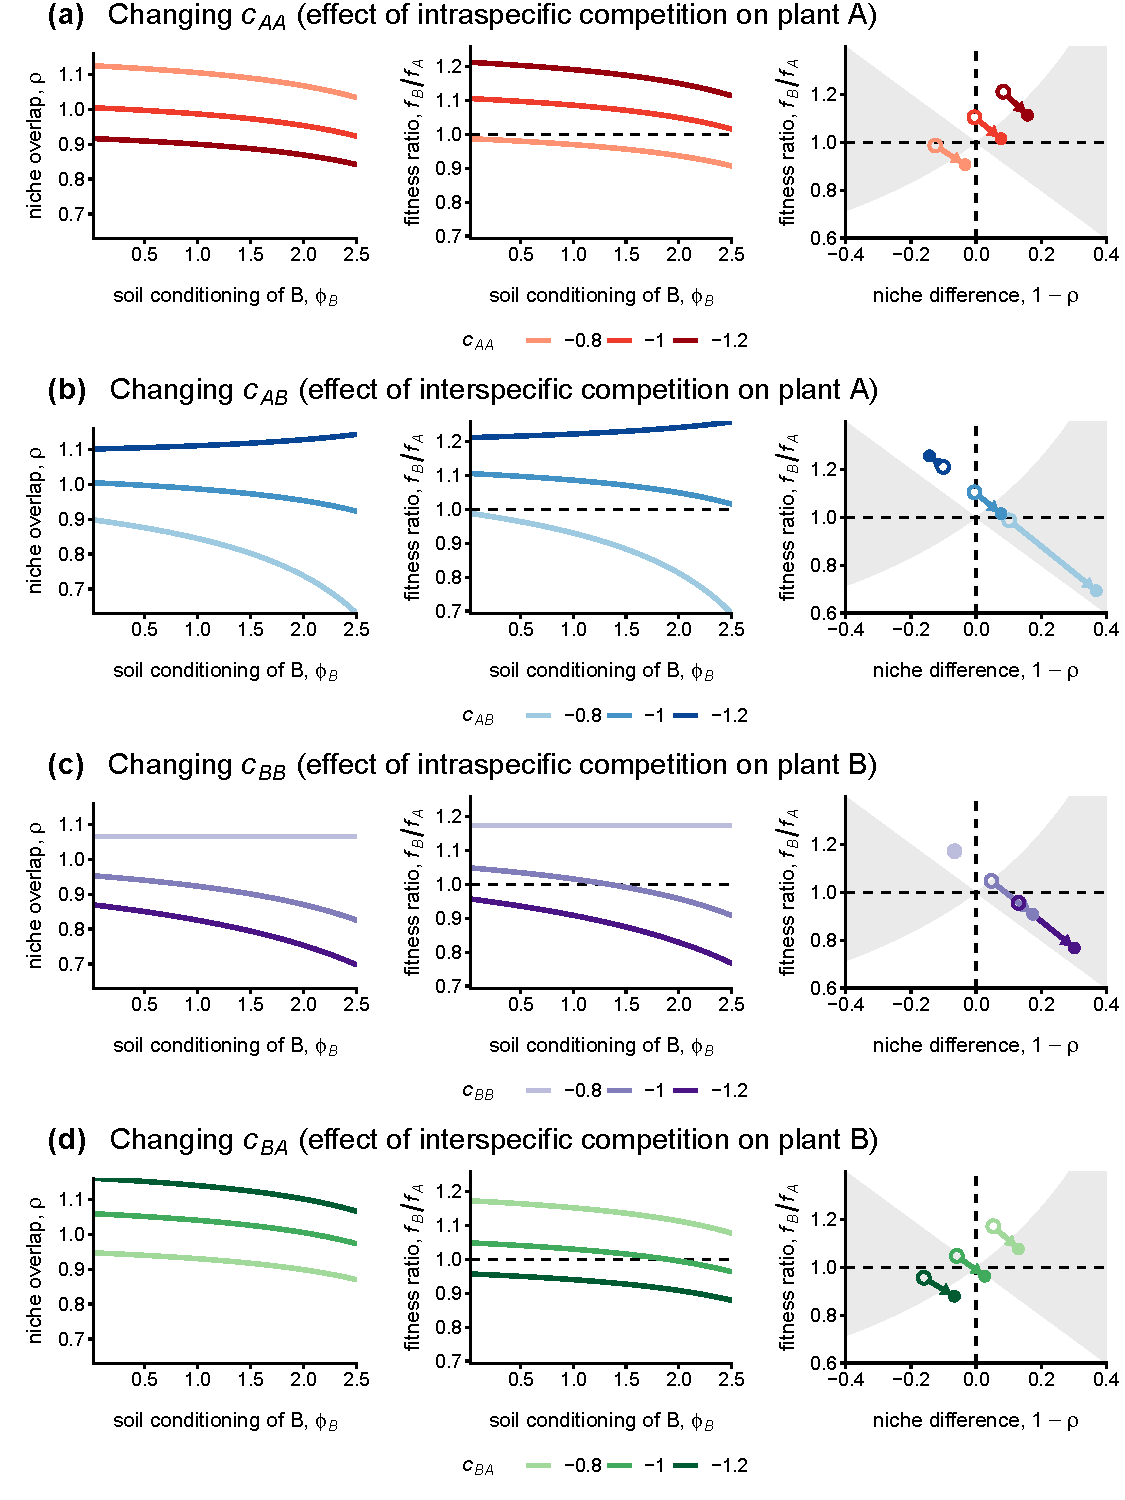
\includegraphics[width=12cm]{Chapter4/Translated_Soil_Conditioning_full.pdf}}
	\caption[The effects of varying plant--soil microbe interactions ($\phi_{B}$) and plant--plant competition on competition outcomes for the differential soil conditioning scenario.]
		{The effects of varying plant--soil microbe interactions ($\phi_{B}$) and plant--plant competition on competition outcomes for the differential soil conditioning scenario.
		Each row (panel a--d) represent the effects of varying one plant--plant competition coefficient while keeping the other three constant: (a) $c_{AA}$, in red colors; (b) $c_{AB}$, in blue colors; (c) $c_{BB}$, in purple colors; (d) $c_{BA}$, in green colors. Lines with different brightness represent different plant--plant competition strength, ranging from weak (light colors) to strong (dark colors).
		The first two columns represent the effects of varying $\phi_{B}$ on niche overlap ($\rho$) and fitness ratio ($f_{B}/f_{A}$), respectively. The third column visualizes the changes in the two components on the parameter space of niche difference ($1 - \rho$, x-axis) and fitness ratio ($f_{B}/f_{A}$, y-axis). Arrows represent the effects of changing plant--soil microbe interactions, from weakest (open circle) to strongest (solid circle). See also Fig.~\ref{fig:Scenario_Battleaxes} legend.}
	\label{fig:Soil_Conditioning_everything}
\end{figure}


\chapter{Testing chronosequence predictions with longitudinal data reveals microbial community convergence: Appendix S1}
%\chaptermark{Positive frequency-dependence}
%\renewcommand{\sectionmark}[1]{}
\fancyhead[LE, RO]{\thepage}
\fancyhead[RE]{APPENDIX D}
\fancyhead[LO]{TESTING CHRONOSEQUENCE WITH LONGITUDINAL DATA}
\fancyfoot{}
\renewcommand{\headrulewidth}{0pt}
\setlength{\parindent}{1cm}


\begin{comment}
\documentclass[hidelinks,12pt]{article}
\usepackage{graphicx,bm, booktabs,lineno,array}
\usepackage[fleqn]{amsmath}
\setlength{\mathindent}{0pt}
\usepackage[super,comma,numbers, compress]{natbib}
\usepackage[a4paper]{geometry}
\usepackage[parfill]{parskip}
\usepackage[usenames,dvipsnames]{color}
\usepackage[font=footnotesize,labelfont=bf,margin=1cm, labelsep = none]{caption} 
\usepackage{setspace}
\usepackage{gensymb}
\usepackage{color} 
\usepackage{sidecap}
\usepackage{epigraph}
\usepackage{float}
\usepackage{soul,xcolor}
\setstcolor{red}
\setlength\epigraphwidth{12cm}
\setlength\epigraphrule{0pt}
\usepackage{etoolbox}
\usepackage{tcolorbox}
\tcbuselibrary{breakable}
\usepackage[bottom, symbol]{footmisc}
\usepackage{authblk}
\usepackage{hyperref}
\usepackage[color=cyan]{todonotes}
\pdfminorversion=3
\doublespacing

\renewcommand{\epigraphflush}{center}
\renewcommand{\sourceflush}{flushleft}
\newcommand{\plus}{\raisebox{.4\height}{\scalebox{.6}{+}}}
\newcommand{\minus}{\raisebox{.4\height}{\scalebox{.8}{-}}}
\renewcommand{\thefootnote}{\fnsymbol{footnote}}
\newcommand*\samethanks[1][\value{footnote}]{\footnotemark[#1]}
\newcommand\blfootnote[1]{%
\begingroup
\renewcommand\thefootnote{}\footnote{#1}%
\addtocounter{footnote}{-1}%
\endgroup
}
\end{comment}



\begin{comment}
\begin{document}
	
\doublespacing
\title{Testing chronosequence predictions with longitudinal data reveals microbial community convergence}
\author[1, $\dagger$]{Po-Ju Ke}
\author[1, 2]{J. Nicholas Hendershot}
\author[1, $\dagger$]{Tadashi Fukami}
\affil[1]{Department of Biology, Stanford University, Stanford, California, USA}
\affil[2]{Center for Conservation Biology, Stanford University, Stanford, California, USA}
 
\date{\today}
\maketitle
\blfootnote{$\dagger$ Correspondence author: Department of Biology, Stanford University, Stanford, California 94305-5020, USA. Phone: +1 650-721-1711. Fax: +1 650-723-6132. Email: pojuke@stanford.edu, fukamit@stanford.edu}
	
\onehalfspacing
\noindent \textbf{Running title:} Predicting community structure with chronosequence\\
\noindent \textbf{Keywords:} beta diversity, \textit{Carpobrotus edulis}, community assembly, sand dunes, space-for-time substitution, succession\\
\noindent \textbf{Type of article:} Research article
	
\begin{myindentpar}{1cm}
	\textbf{Words in Abstract:} $\sim$ 200\\
	\textbf{Words in main text:} $\sim$ XXX\\
	\textbf{Number of references:} $\sim$ 50\\
	\textbf{Number of figures:} 5\\
\end{myindentpar}
	
\noindent \textbf{Authorship statement:} PJK and TF conceived the study; PJK conducted the study; PJK and JNH analyzed the data; PJK wrote the first draft of the manuscript with substantial contribution from all authors.\\
	
\noindent \textbf{Data accessibility statement:} Should the manuscript be accepted, all data and computer scripts supporting the results will be archived in a public repository, with the DOI included in the article.\\

\linenumbers
\doublespacing
\end{comment}



\section{Appendix S1 -- Supplementary Figures}
\clearpage
\begin{sidewaysfigure}[h]
	\centering
	\makebox[\textwidth][c]{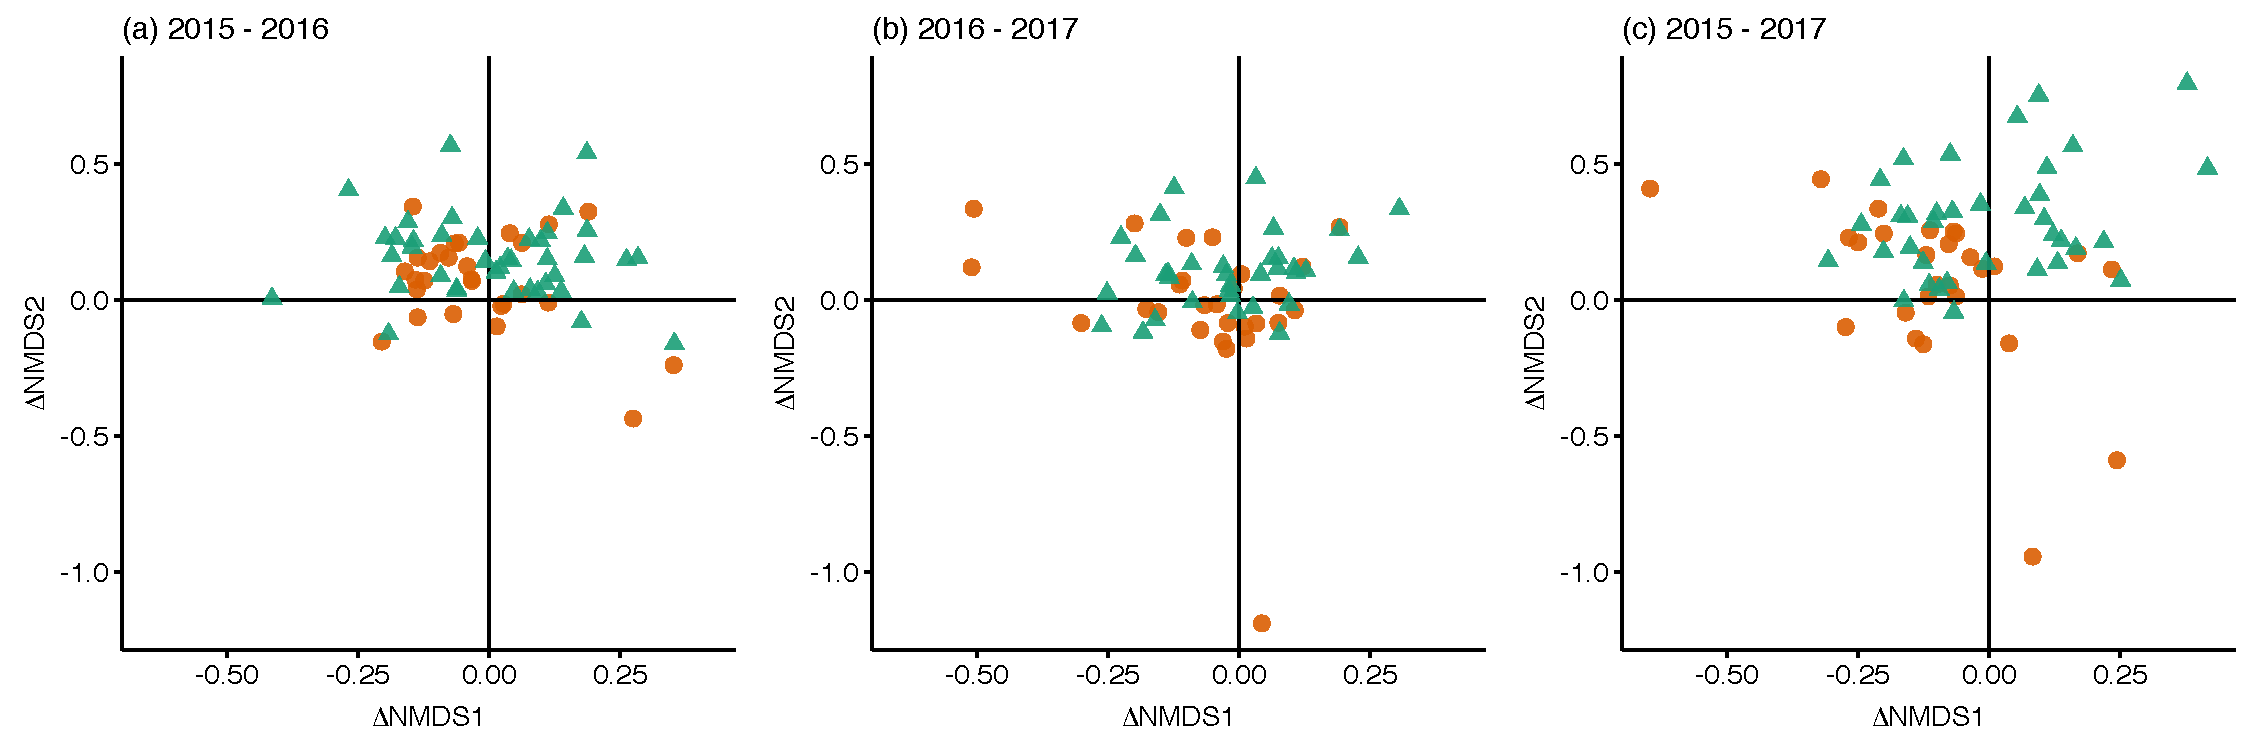
\includegraphics[width=18cm]{Chapter5/FourQuadrateMovement_Species_Common_RevisedSI.pdf}}
	\caption[Compositional shifts in fungal communities from the same plant individual among different sampling years.]
		{\hspace{1mm} Compositional shifts in fungal communities from the same plant individual among different sampling years. Each point represent the movement (i.e., x- and y-component of the arrow) on Fig.~\ref{fig:3YrNMDS_Individual}. A positive x-component (i.e., $\Delta$NMDS 1 $ > 0$) and y-component (i.e., $\Delta$NMDS 2 $ > 0$) represents a rightward and upward movement, respectively. (a) Shifts from 2015 to 2016; (b) shifts from 2016 to 2017; (c) shifts representing compositional differences between 2015 and 2017 (i.e., Fig.~\ref{fig:FourQuadrate_Individual_Species}). Point shapes and colors represent plant species (orange circle: \textit{C. edulis}; green triangle: \textit{L. arboreus}). 
		% See Fig.~\ref{fig:FourQuadrate_Sample_Species} for identical pattern when soil samples were plotted as observation units.
		}
	\label{fig:FourQuadrate_Individual_Species_SI}
\end{sidewaysfigure}



\clearpage
\begin{figure}[h]
	\centering
	\makebox[\textwidth][c]{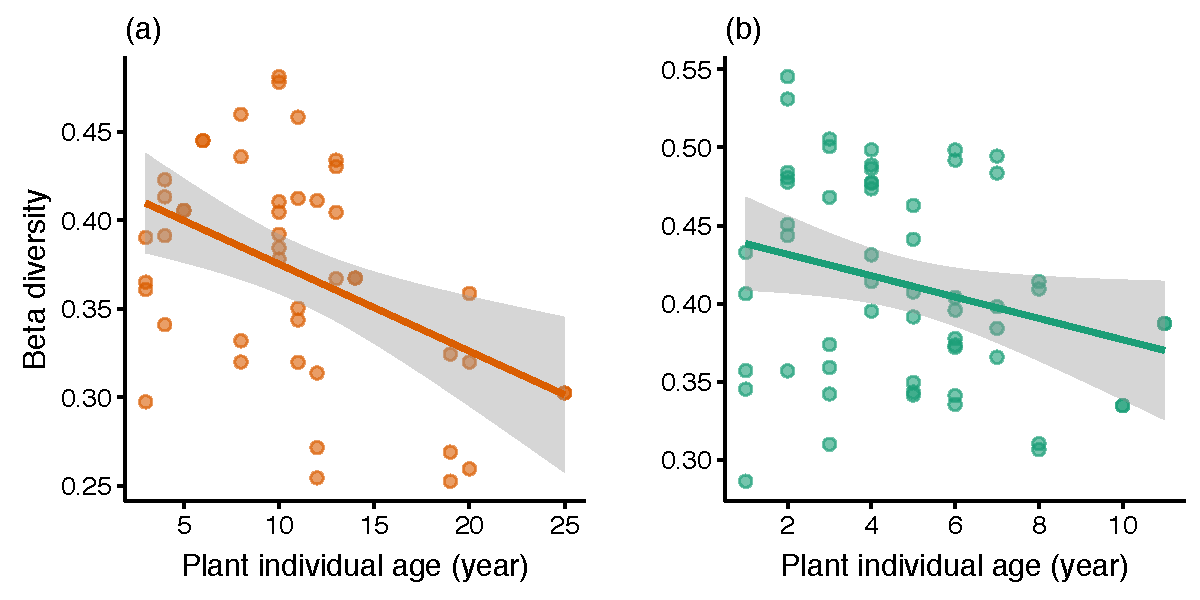
\includegraphics[width=15cm]{Chapter5/BetaDiversity_CompiledFull2015_Common_RevisedSI.pdf}}
	\caption[The relationship between plant age and beta diversity of fungal communities associated with chronosequence plant individuals.]
		{\hspace{1mm} The relationship between plant age and beta diversity of fungal communities associated with chronosequence plant individuals.
		(a) and (b) show the pattern for microbial communities associated with \textit{C. edulis} (orange) and \textit{L. arboreus} (green), respectively. 
		Each point represents the distance of one fungal community to the age-specific centroid.  
		% See Fig.~\ref{fig:Full2015Beta_Sample} for the pattern when soil samples were plotted as observation units.
		} 
	\label{fig:CombinedFull2015Beta_Individual_SI}
\end{figure}



\clearpage
\begin{figure}[h]
	\centering
	\makebox[\textwidth][c]{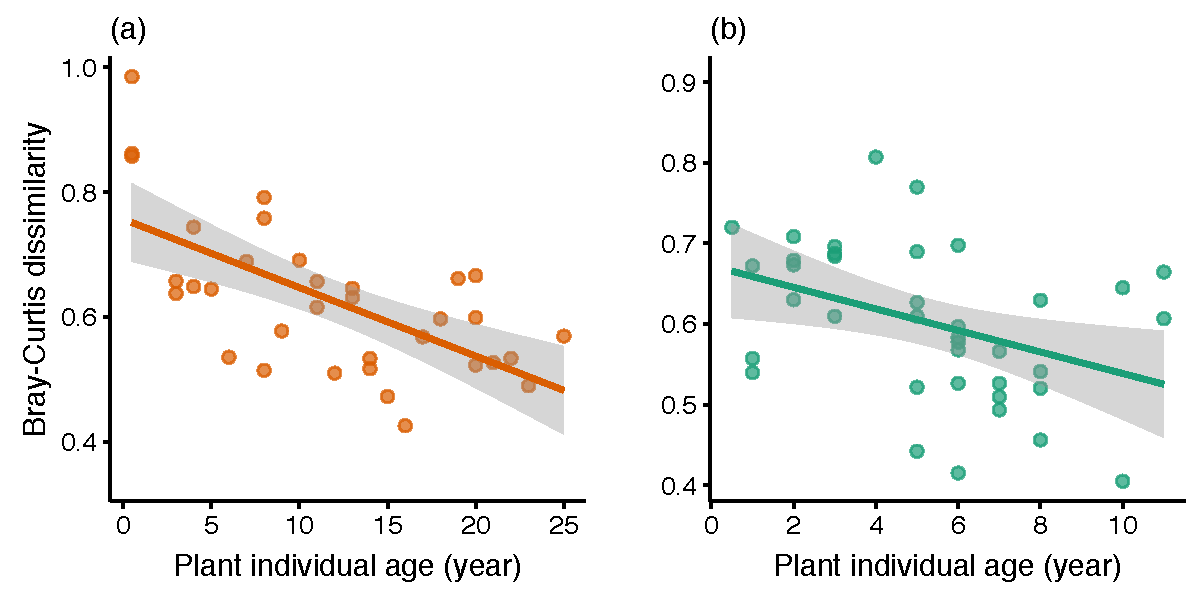
\includegraphics[width=15cm]{Chapter5/Goodness_FungiSpecies_CombinedIndividual_Full2015glmmTMBTotal_Revised2SI.pdf}}
	\caption[The relationship between plant age and Bray--Curtis dissimilarity between the fungal community observed in 2017 and the 2015 chronosequence prediction.]
		{\hspace{1mm} The relationship between plant age and Bray--Curtis dissimilarity between the fungal community observed in 2017 and the 2015 chronosequence prediction.
		(a) and (b) show the pattern for microbial communities associated with \textit{C. edulis} (orange) and \textit{L. arboreus} (green), respectively.
		Each point represents the dissimilarity calculated for a fungal community, using samples collected in 2017 as the validation test set. 
		% See Fig.~\ref{fig:HMSC_Species_Sample_Full2015} or identical pattern when soil samples were plotted as observation units.
		}
	\label{fig:HMSC_Species_Individual_Full2015_SI}
\end{figure}



\clearpage
\begin{figure}[h]
	\vspace*{-1cm}
	\centering
	\makebox[\textwidth][c]{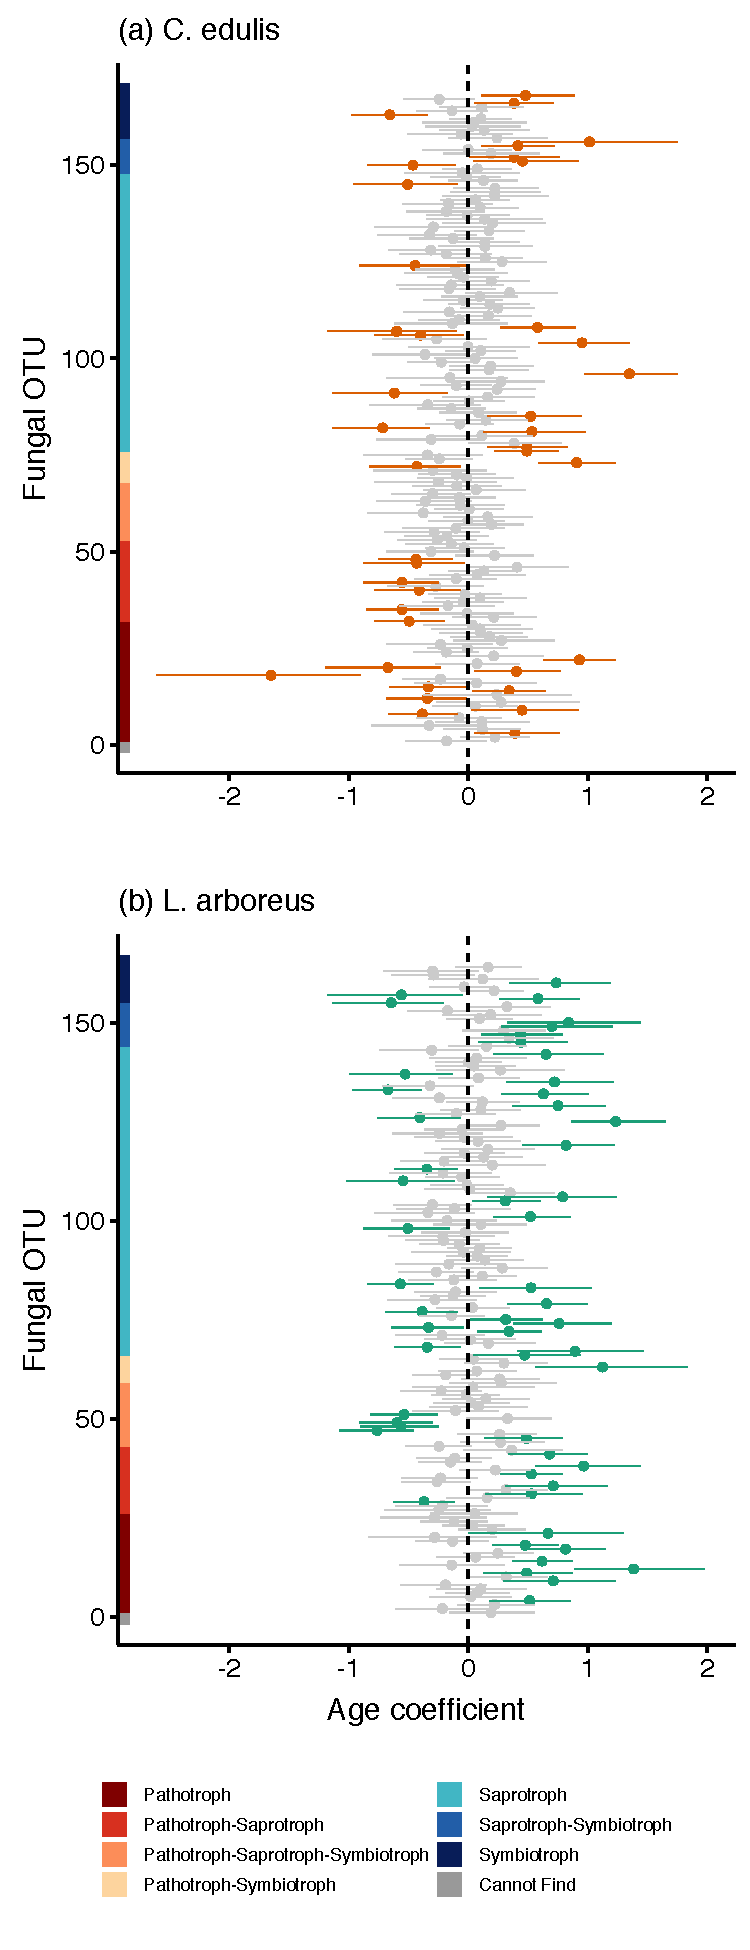
\includegraphics[width=7cm]{Chapter5/Funguild_HMSC_FungiSpecies_CombinedIndividual_Full2015Total_Long.pdf}}
	\caption[Predicted temporal trends and potential functional guilds of fungal OTUs associated with \textit{C. edulis} and \textit{L. arboreus}.]
		{\hspace{1mm} Predicted temporal trends and potential functional guilds of fungal OTUs associated with (a) \textit{C. edulis} and (b) \textit{L. arboreus}. Model fitting was performed for the two plant species separately. Points and line segments represent the mean and the 95$\%$ credible interval of the fitted age coefficient (x-axis) for different fungal OTUs (y-axis). Significant age coefficients are colored (orange for \textit{C. edulis}; green for \textit{L. arboreus}) and insignificant ones are in gray. Color codes along the y-axis are the predicted functional guild of the OTU obtained from \textit{FunGuild}.}
	\label{fig:Funguild_HMSC_Species_Individual_Full2015}
\end{figure}


\chapter{Dynamic plant--soil microbe interactions: the neglected effect of soil conditioning time: Appendices S1--S2}
%\chaptermark{Positive frequency-dependence}
%\renewcommand{\sectionmark}[1]{}
\fancyhead[LE, RO]{\thepage}
\fancyhead[RE]{APPENDIX E}
\fancyhead[LO]{TEMPORAL PLANT--SOIL FEEDBACK}
\fancyfoot{}
\renewcommand{\headrulewidth}{0pt}
\setlength{\parindent}{1cm}


\begin{comment}
\documentclass[hidelinks,12pt]{article}
\usepackage{graphicx,bm, booktabs,lineno,array}
\usepackage[fleqn]{amsmath}
\setlength{\mathindent}{0pt}
\usepackage[super,comma,numbers, compress]{natbib}
\usepackage[a4paper]{geometry}
\usepackage[parfill]{parskip}
\usepackage[usenames,dvipsnames]{color}
\usepackage[font=footnotesize,labelfont=bf,margin=1cm, labelsep = none]{caption} 
\usepackage{setspace}
\usepackage{gensymb}
\usepackage{color} 
\usepackage{sidecap}
\usepackage{epigraph}
\usepackage{float}
\usepackage{soul,xcolor}
\setstcolor{red}
\setlength\epigraphwidth{12cm}
\setlength\epigraphrule{0pt}
\usepackage{etoolbox}
\usepackage{tcolorbox}
\tcbuselibrary{breakable}
\usepackage[bottom, symbol]{footmisc}
\usepackage{authblk}
\usepackage{hyperref}
\usepackage[color=cyan]{todonotes}
\pdfminorversion=3
\doublespacing

\renewcommand{\epigraphflush}{center}
\renewcommand{\sourceflush}{flushleft}
\newcommand{\plus}{\raisebox{.4\height}{\scalebox{.6}{+}}}
\newcommand{\minus}{\raisebox{.4\height}{\scalebox{.8}{-}}}
\renewcommand{\thefootnote}{\fnsymbol{footnote}}
\newcommand*\samethanks[1][\value{footnote}]{\footnotemark[#1]}
\newcommand\blfootnote[1]{%
\begingroup
\renewcommand\thefootnote{}\footnote{#1}%
\addtocounter{footnote}{-1}%
\endgroup
}
\end{comment}



\begin{comment}
\title{Coexistence theory and the frequency-dependence of priority effects}
\author[1]{Po-Ju Ke \thanks{Both authors contributed equally.}}
\author[1,2,3]{Andrew D. Letten \samethanks}
\affil[1]{Department of Biology, Stanford University, Stanford, California, 94305-5020, USA}
\affil[2]{Centre for Integrative Ecology, University of Canterbury, Christchurch, New Zealand}
\affil[3]{Institute of Integrative Biology, Department of Environmental Systems Science, ETH Z{\"u}rich, 8092 Z{\"u}rich, Switzerland}

\begin{document}

\date{}
\maketitle
\blfootnote{Correspondence email: pojuke@stanford.edu, andrew.letten@usys.ethz.ch}
%\textbf{Running title:} PFD
%\textbf{Keywords:} No key words for Forum 
\textbf{Type of article:} Brief Communication\\
\textbf{Number of words:} 1847 [main text] \\
\textbf{References:} 17\\
\textbf{Display items:} 3\\
\end{comment}



\section{Appendix S1 -- Detailed methods}
\subsection{DNA sequencing of fungal and bacterial communities}
We extracted microbial DNA from 0.25 g of subsampled soil with PowerSoil DNA Isolation Kit (Qiagen) following the manufacturer's protocol. We then amplified the bacterial 16S ribosomal DNA region, with primer pair 515f (5$^\prime$- GTG YCA GCM GCC GCG GTA A -3$^\prime$) -- 806r (5$^\prime$- GGA CTA CNV GGG TWT CTA AT -3$^\prime$) \citep{Caporaso2012}, and the fungal internal transcribed spacer 1 region (ITS1), with primer pair ITS1-F$\textunderscore$KYO1 (5$^\prime$- CTH GGT CAT TTA GAG GAA STA A -3$^\prime$) -- ITS2$\textunderscore$KYO2 (5$^\prime$- TTY RCT RCG TTC TTC ATC -3$^\prime$) \citep{Toju2012}. Each primer was concatenated with 3 -- 6-mer Ns \citep{Lundberg2013} and an Illumina sequencing primer region, resulting in a fusion primer for our PCR reactions (forward: 5$^\prime$- TCG TCG GCA GCG TCA GAT GTG TAT AAG AGA CAG -- [3--6-mer Ns] -- [515f or ITS1-F$\textunderscore$KYO1] -3$^\prime$; reverse: 5$^\prime$- GTC TCG TGG GCT CGG AGA TGT GTA TAA GAG ACA G -- [3--6-mer Ns] -- [806r or ITS2$\textunderscore$KYO2] -3$^\prime$). 
\par


Our 10 $\mu$L PCR reaction contained 3.2 $\mu$L of MQ water, 5 $\mu$L of MyTaq HS DNA polymerase Mastermix (Bioline), 0.4 $\mu$L of each primer (10$\mu$M for both forward and reverse primer), and 1 $\mu$L of extracted DNA. We ran the reactions at 95$^{\circ}$C for 2 min, followed by 36 cycles of 95$^{\circ}$C for 20 sec, 52.5$^{\circ}$C for 16S (or 50$^{\circ}$C for ITS1) for 20 sec, 72$^{\circ}$C for 50 sec, and a final extension at 72$^{\circ}$C for 10 min. A ramp rate of 1$^{\circ}$C/s was set to prevent chimeric amplicon generation. After this first PCR process, we ran a subsequent second PCR for sample identification. The fusion primers used in this second PCR concatenates P5/P7 Illumina adaptors, 8-mer index sequences, and the sequencing adaptor \citep{Hamady2008} (forward: 5$^\prime$- AAT GAT ACG GCG ACC ACC GAG ATC TAC AC -- [8-mer tag] -- TCG TCG GCA GCG TC -3$^\prime$; reverse: 5$^\prime$- CAA GCA GAA GAC GGC ATA CGA GAT -- [8-mer tag] -- GTC TCG TGG GCT CGG -3$^\prime$). The second PCR was run for 8 cycles with the same temperature profile as our first PCR but with an annealing temperature of 50$^{\circ}$C for both bacterial 16S and fungal ITS1 amplicons. After a purification/equalization process with the AMPure XP Kit (with a sample : AMpureXP ratio = 1 : 0.6, Agencourt), 5$\mu$L of PCR product were taken from each sample to create a pooled library. This library was then sequenced using the Illumina MiSeq sequencer at the Stanford Functional Genomics Facility (2 $\times$ 250 cycle sequencing kit) with 15$\%$ PhiX spike-in.
\par


The raw Illumina MiSeq sequencing reads were processed with the Claident pipeline (\citealp{Tanabe2013}, v0.2.2015.11.19). To prevent potential mis-tagging, demultiplexing was conducted within Claident after converting raw Miseq BCL data into FASTQ data with the program bcl2fastq v1.8.4. All sequencing reads with low quality scores ($<$ 30) were deleted. The obtained forward and reverse sequencing reads were fused with each other by the program PEAR v0.9.6 \citep{Zhang2014} and merged reads with low quality (quality score $<$ 30 or length $<$ 150 bp) were deleted. Potentially chimeric and noisy reads were also eliminated with the program UCHIME v4.2 \citep{Edgar2011}. Sequencing reads that passed through all filtering processes were then clustered into operational taxonomic units (OTUs), with a cutoff sequence similarity of 97$\%$, with the program VSEARCH (\citealp{Rognes2016}, implemented in Claident). This clustering process resulted in 19,868 OTUs representing 1,772,220 sequences for ITS1 sequencing reads and 164,983 OTUs representing 3,512,717 sequences for 16S sequencing reads. After clustering, fungal and bacterial OTUs with less than ten total sequencing reads were removed. Taxonomy was assigned to the remaining OTUs using the RDP Naive Bayesian rRNA Classifier v2.11 \citep{Wang2007} trained on either the 16S rRNA training set 16 for bacteria or the Warcup Fungal ITS training set 2 \citep{Deshpande2016} for fungi. Based on the taxonomic assignment results, ITS1(16S) sequences other than those of the Kingdom fungi (bacteria) were removed from the dataset. For both ITS and 16S datasets, potential contaminant OTUs were identified statistically based on their prevalence in PCR and extraction negative controls (two of each for every 96 well plate reaction) using the R package decontam \citep{Davis2018}.This resulted in the elimination of 36 fungal ITS and 22 bacterial 16S OTUs. Finally, before any downstream analyses presented in this study, the OTU tables were rarefied to 1,000 sequencing reads \citep{McMurdie2013}. For fungal communities, the rarefaction process deleted 1 \textit{B. pilularis} individual and 6 sand samples.
\par


\subsection{Statistical analysis of microbial communities}
To identify the fungal and bacterial taxonomic groups that are driving the observed community pattern, we applied a model-based approach with the R package HMSC \citep{Ovaskainen2017}. 
To ensure adequate model fit, we aggregated the microbial communities to the family level and constrained this analysis to fungal and bacterial families that belonged to the top ten abundant phyla and occurred in more than 20$\%$ of the samples. 
Different from other analyses, this model fitting was performed by treating each soil sample as replicate units in order to take advantage of the hierarchical Bayesian approach implemented in \textit{HMSC} \citep{Ovaskainen2017}. 
We assumed that the abundance of each fungal and bacterial class follows an over-dispersed Poisson distribution and fitted models with plant age as fixed effect and plant individual as random effect. 
For all models, the MCMC sampling was conducted for 1,000,000 iterations, with a burn-in phase of 500,000 iterations and thinned every 100 iterations.
All model fitting was performed separately for each plant species. This is because plants vary in their longevity and thus the same age does not necessarily represent the same life stage for different plants.
The mean and the 95$\%$ credible interval of the age coefficient's marginal posterior distributions were summarized and plotted for each plant species separately.
\par


\subsection{Greenhouse experiment}
Our greenhouse experiment used soil samples collected in July 2017 and was separated into two rounds, which started in late August and September 2017, respectively. The range and variance of age of individuals were kept similar among the two rounds. To avoid arbitrarily averaging soil conditions \citep{Rinella2018}, soils collected from different individuals were kept separated throughout the experiment. Half of the volume (150 mL) collected from each individual was autoclaved to create a sterile treatment (120$^\circ$C for 60 min, sit overnight for 24 h, and another 120$^\circ$C for 60 min). Due to handling mistakes, we had to discard soil inocula collected from 9 individuals: 6 in the first round (i.e., soils from 1 individual of \textit{A. arenaria}, 3 individuals of \textit{C. edulis}, and 2 individuals of \textit{L. arboreus}), and 3 in the second round (i.e., soils from 2 individuals of \textit{B. pilularis} and 1 individual of \textit{C. edulis}). Two rounds combined, we ended up with 222 unique soil environments: 108 in the first round (i.e., (14 \textit{A. arenaria} + 15 \textit{B. pilularis} + 12 \textit{C. edulis} + 13 \textit{L. arboreus}) individuals $\times$ 2 sterilization treatments), and 114 in the second round (i.e., (15 \textit{A. arenaria} + 13 \textit{B. pilularis} + 14 \textit{C. edulis} + 15 \textit{L. arboreus}) individuals $\times$ 2 sterilization treatments).
\par


Plant seeds were purchased from commercial seed suppliers (i.e., \textit{A. arenaria}: Jelitto perennial seeds; \textit{B. pilularis}: Larner seeds; \textit{C. edulis}: independent donor; \textit{L. arboreus}: J.L. Hudson, Seedsman). The seeds were surface sterilized by soaking seeds in 5$\%$ bleach for 30 sec, 95$\%$ ethanol for 30 sec, and rinsing them with DI water for 1 min. The sterilized seeds were spread evenly onto germination trays filled with sterilized sand (1:1 mixing of sterile play sand and Lapis Lustre $\#$ 2/12 sand (Cemex) to mimic the soil particle distribution in the field), and placed in a growth chamber (16-hr/8-hr light/dark, and temperature held at 16$^\circ$C). After two weeks, we transplanted the seedlings individually into 107 mL "cone-tainers" pots (hereafter "pots"; Stuewe and Sons) filled with 80 mL of sterilized sand (prepared with the same method as for germination) and added 20 mL of either live or sterile soil inoculum to the top. Three of the four species were transplanted in both experimental rounds, with \textit{B. pilularis} being the exception due to low germination rate during the second round. The final number of pots was 774, consisting of 432 from the first round (i.e., 54 individuals $\times$ 2 sterilization treatments $\times$ 4 species) and 342 from the second round (i.e., 57 individuals $\times$ 2 sterilization treatments $\times$ 3 species).
\par

 
Transplanted pots were randomly placed onto every other cell of 98 well trays (to avoid crowding), and were grown in the greenhouse for 12 weeks (14-hr/10-hr light/dark with ambient temperature). To mimic precipitation regimes in the field, which is mainly fog during the summers, 30 sec brief water spray with automatic misting nozzles were applied every hour. Seedlings that died within the first 10 days were replanted, and for seedlings that died afterwards their live--sterile soil pair were discarded from the calculation of microbial effects. Two rounds combined, data for 20 live--sterile soil pairs were discarded due to the death of seedlings or handling mistakes: 3 seedlings of \textit{A. arenaria} (i.e., 1 in \textit{A. arenaria} soil, 1 in \textit{B. pilularis} soil, 1 in \textit{L. arboreus} soil), 5 seedlings of \textit{B. pilularis} (i.e., 2 in \textit{A. arenaria} soil, 1 in \textit{B. pilularis} soil, 1 in \textit{C. edulis} soil, 1 in \textit{L. arboreus} soil), 9 seedlings of \textit{C. edulis} (i.e., 2 in \textit{A. arenaria} soil, 3 in \textit{B. pilularis} soil, 2 in \textit{C. edulis} soil, 2 in \textit{L. arboreus} soil), and 3 seedlings of \textit{L. arboreus} (i.e., 1 in \textit{B. pilularis} soil, 1 in \textit{C. edulis} soil, 1 in \textit{L. arboreus} soil). After 12 weeks, we harvested all above- and below-ground tissue from each pot, carefully rinsed soil off the root system, and oven-dried tissue at 70$^{\circ}$C for 96 h. 
% Ambient temperature for August--September: mean daily maximum is 29.8$^\circ$C and mean daily  minimum is 18.1$^\circ$C,
\par



\subsection{Simulation model}
\subsubsection*{Overview}
To investigate the potential long-term effects of temporally-varying plant--soil microbe interactions on plant community dynamics, we constructed an individual-based model following the model in  \citet{FukamiNakajima2011} (see also \citealp{Fukami2013, ZeeFukami2015, Fukami2017}). The model simulates the immigration, reproduction, arrival, establishment, and death of plant individuals. 
In our model, plant propagules consist of immigration from a regional species pool and seed production dispersed from established plants. These propagules compete for the establishment at empty sites, where species' competitive ability is determined by the habitat condition of the site, species' trait, and the legacy soil microbial effects (i.e., plant--soil microbe interactions) imposed by the previously established plant species. 
Established individuals die with a fixed mortality rate and those that survived can produce propagules next year to colonize empty sites, which are released as individuals die.
We simulated the community assembly process for multiple years, repeating the above processes until a stable state was reached. All simulation runs were performed in \textit{R} version 3.3.1 \citep{R}. 
\par


\subsubsection*{Species pool and landscape}
For each round of simulated community assembly, we considered a regional species pools containing 50 plant species. Each species $i$ is characterized by a trait value, $R_{i}$, chosen randomly from a uniform distribution $U\left ( 0, 1 \right )$. Species are also characterized by a set of plant--soil microbe interaction values, $S_{ij}^{\tau}$. These values quantify how the previously-established plant species $j$, which died at age $\tau$, affect the competitive ability of plant species $i$ (see section \textit{Plant-soil interactions}). 
One patch in our simulation consists of 1024 local sites, arranged in a one-dimensional circular array, for plant individuals to colonize. Local site are characterized by a habitat condition value, $H_{k}$, chosen randomly from a beta-distribution with shape parameters $\alpha = \beta = 50$. This setting yielded many local sites having $H_{k}$ values close to 0.5 and few close to either 0 or 1. 
\par


\subsubsection*{Community assembly}
We started our simulation from an empty patch, allowing plant propagules to colonize empty local sites. In our model, plant propagules consist of immigrants from the regional species pool and seeds produced and dispersed from established plants.
Each year, species in the regional species pool immigrate to the patch with equal probability, $p_{I} = 0.05$. Selected immigrating species produce $f_{I} = 10$ propagules that disperse globally, i.e., the propagule can land at any local site with equal probability.
In addition to immigration, established individuals contribute to the propagule rain by seed production. We assumed that all established individuals reproduce at each time step (i.e., $p_{R} = 1$) and reproducing individuals have a fecundity of $f_{R} = 5$.
We assumed that seeds produced by established individuals have limited dispersal ability: the landing locations of seeds were drawn independently from a Gaussian distribution with a mean at the location of its reproducing parent and a variance of $\sigma_{R}$, which determines how far seeds can disperse. We set $\sigma_{R} = 150$ to represent intermediate dispersal distance \citep{ZeeFukami2015}.
Propagules that landed at local sites with an established individual will perish as they cannot displace the resident, whereas those that landed at an empty local site would have a chance to establish.
To highlight the effects of soil microbial legacies, demographic parameters mentioned above were set equal for all species.
\par


When more than one propagule landed at the same empty site, the propagule belonging to the species with the highest value of competitiveness, $C_{ijk}^{\tau}$, will successfully establish. 
Modified from \citet{Fukami2013}, we defined $C_{ijk}^{\tau}$ of species $i$ at site $k$, which was made vacant during the previous time step when species $j$ died, as $C_{ijk}^{\tau} = \left ( 1 - \left | H_{k} - Z_{i} \right | \right )S_{ij}^{\tau}$. 
The term within the parenthesis measures the relative fit of species $i$ to the habitat condition at site $k$, i.e., species with a closer trait value--habitat condition match are superior competitors. 
This term is modulated by $S_{ij}^{\tau}$, which captures the soil microbial legacy effect that an aged-$\tau$ species $j$ individual imposes on the newly-arrived species $i$ propagule. The superscript $\tau$ indicates the age-at-death, and thus the length of soil conditioning, of species $j$, which is an important determinant of the plant--soil microbe interaction strength (see section \textit{Plant-soil interactions}).
After competition for establishment was completed, individuals die with a mortality rate, $m$, which is set equal as 0.2 for all species. As we assumed replacement competition, an established individual will persist until its stochastic death, regardless of whether more competitive propagules arrive later at its site.
We assembled communities by following these rules of immigration, reproduction, arrival, establishment, and death for $t = 2000$ years. 
\par


\subsubsection*{Age-dependent plant--soil interactions}
The value of $S_{ij}^{\tau}$ captures the direction and strength of soil microbial legacy effects that an individual of species $j$, which died at the age of $\tau$, imposes on species $i$. A value of 1 indicates no microbial effects as it does not modify the competitiveness of species $i$. A value greater than 1 indicates positive microbial effects (e.g., facilitation through beneficial microbes), whereas a value less than 1 indicates negative microbial effects (e.g., antagonism through detrimental pathogens). Following \citet{Fukami2013}, we considered four types of plant--soil microbe interactions: 
(1) `no interactions', where $S_{ij}^{1}$ (i.e., the initial microbial effect generated by an individual that only survived for one year) is 1 for all pairs of species $i$ and $j$; 
(2) `positive conspecific interactions', where $S_{ij}^{1}$ is chosen randomly from a uniform distribution $U\left ( 1.0, 1.5 \right )$ when $i = j$ but equals 1 when $i \neq j$; 
(3) `negative conspecific interactions', where $S_{ij}^{1}$ is chosen randomly from $U\left ( 0.5, 1.0 \right )$ when $i = j$ but equals 1 when $i \neq j$; 
(4) `complex plant--soil microbe interactions', where $S_{ij}^{1}$ is chosen randomly from $U\left ( 0.5, 1.0 \right )$ when $i = j$ and from $U\left ( 0.5, 1.5 \right )$ when $i \neq j$ (i.e., conspecific interactions are negative whereas heterospecific ones can be either positive or negative).
\par


To incorporate age-dependent plant--soil microbe interactions, we considered four temporal development scenarios of $S_{ij}^{\tau}$: 
(1) `constant', where the microbial effect remains at its initial $S_{ij}^{1}$ value and is independent to the age-at-death, $\tau$, of the individual of species $j$; 
(2) `magnifying', where positive and negative microbial effects intensify in their strengths with greater age-at-death of the individual of species $j$ (i.e., $S_{ij}^{\tau}$ start from its initial $S_{ij}^{1}$ value and intensify towards its biological extremes, 1.5 and 0.5 for positive and negative microbial effects, respectively, with increasing $\tau$); 
(3) `decaying', where positive and negative microbial effects attenuate with greater age-at-death of the individual of species $j$ (i.e., $S_{ij}^{\tau}$ start from its initial $S_{ij}^{1}$ value and decay towards 1 with increasing $\tau$); 
(4) `bidirectionally varying', where $S_{ij}^{1}$ has equal probability to either intensify (towards biological extremes) or attenuate (towards no feedback) with increasing $\tau$.
For scenarios (2)--(4), we assumed that changes in $S_{ij}^{\tau}$ follow a linear function and set the rate of change to 0.1 per year. 
A schematic description of microbial effects varying through time is given in Fig.~\ref{fig:SimulationComplexPSF}.
\par


\subsubsection*{Simulation exercise and calculating species diversity}
We focused on the effects of different temporal development scenarios on plant community convergence.
For each of the four plant--soil microbe interactions types (i.e., no interactions, positive, negative, and complex interactions), we generated one set of initial plant--soil interaction matrix (i.e., $S_{ij}^{1}$ values) and ran simulations with $S_{ij}^{\tau}$ values following different temporal development scenarios (i.e., constant, magnifying, decaying, and bidirectionally varying).
In total, our simulation resulted in 13 interaction type $\times$ temporal development combinations since the no interaction simulations can only remain constant through time.
For our whole simulation exercise, we generated 10 patches for the regional species pools to colonize independently and quantified changes in species diversity indexes through time. 
We measured alpha-diversity as the average number of species presented in the 10 patches, and gamma-diversity as the number of species presented in at least one patch. We measured beta-diversity as the gamma-diversity divided by the averaged alpha-diversity, which can be viewed as a proxy of the effective number of distinct local communities in the region \citep{FukamiNakajima2011}.
For each interaction type $\times$ temporal development combination, the above simulation was replicated 20 times, where 20 independently-created sets of regional species pool were allowed to colonize the same set of 10 patches, using the same set of $S_{ij}^{1}$ values for each plant--soil microbe interaction type. We then compared the mean beta-diversity and the temporal trajectory among different temporal development scenarios.
\par



\clearpage
\section{Appendix S2 -- Supplementary Figures}
\begin{figure}[h]
	\centering
	\makebox[\textwidth][c]{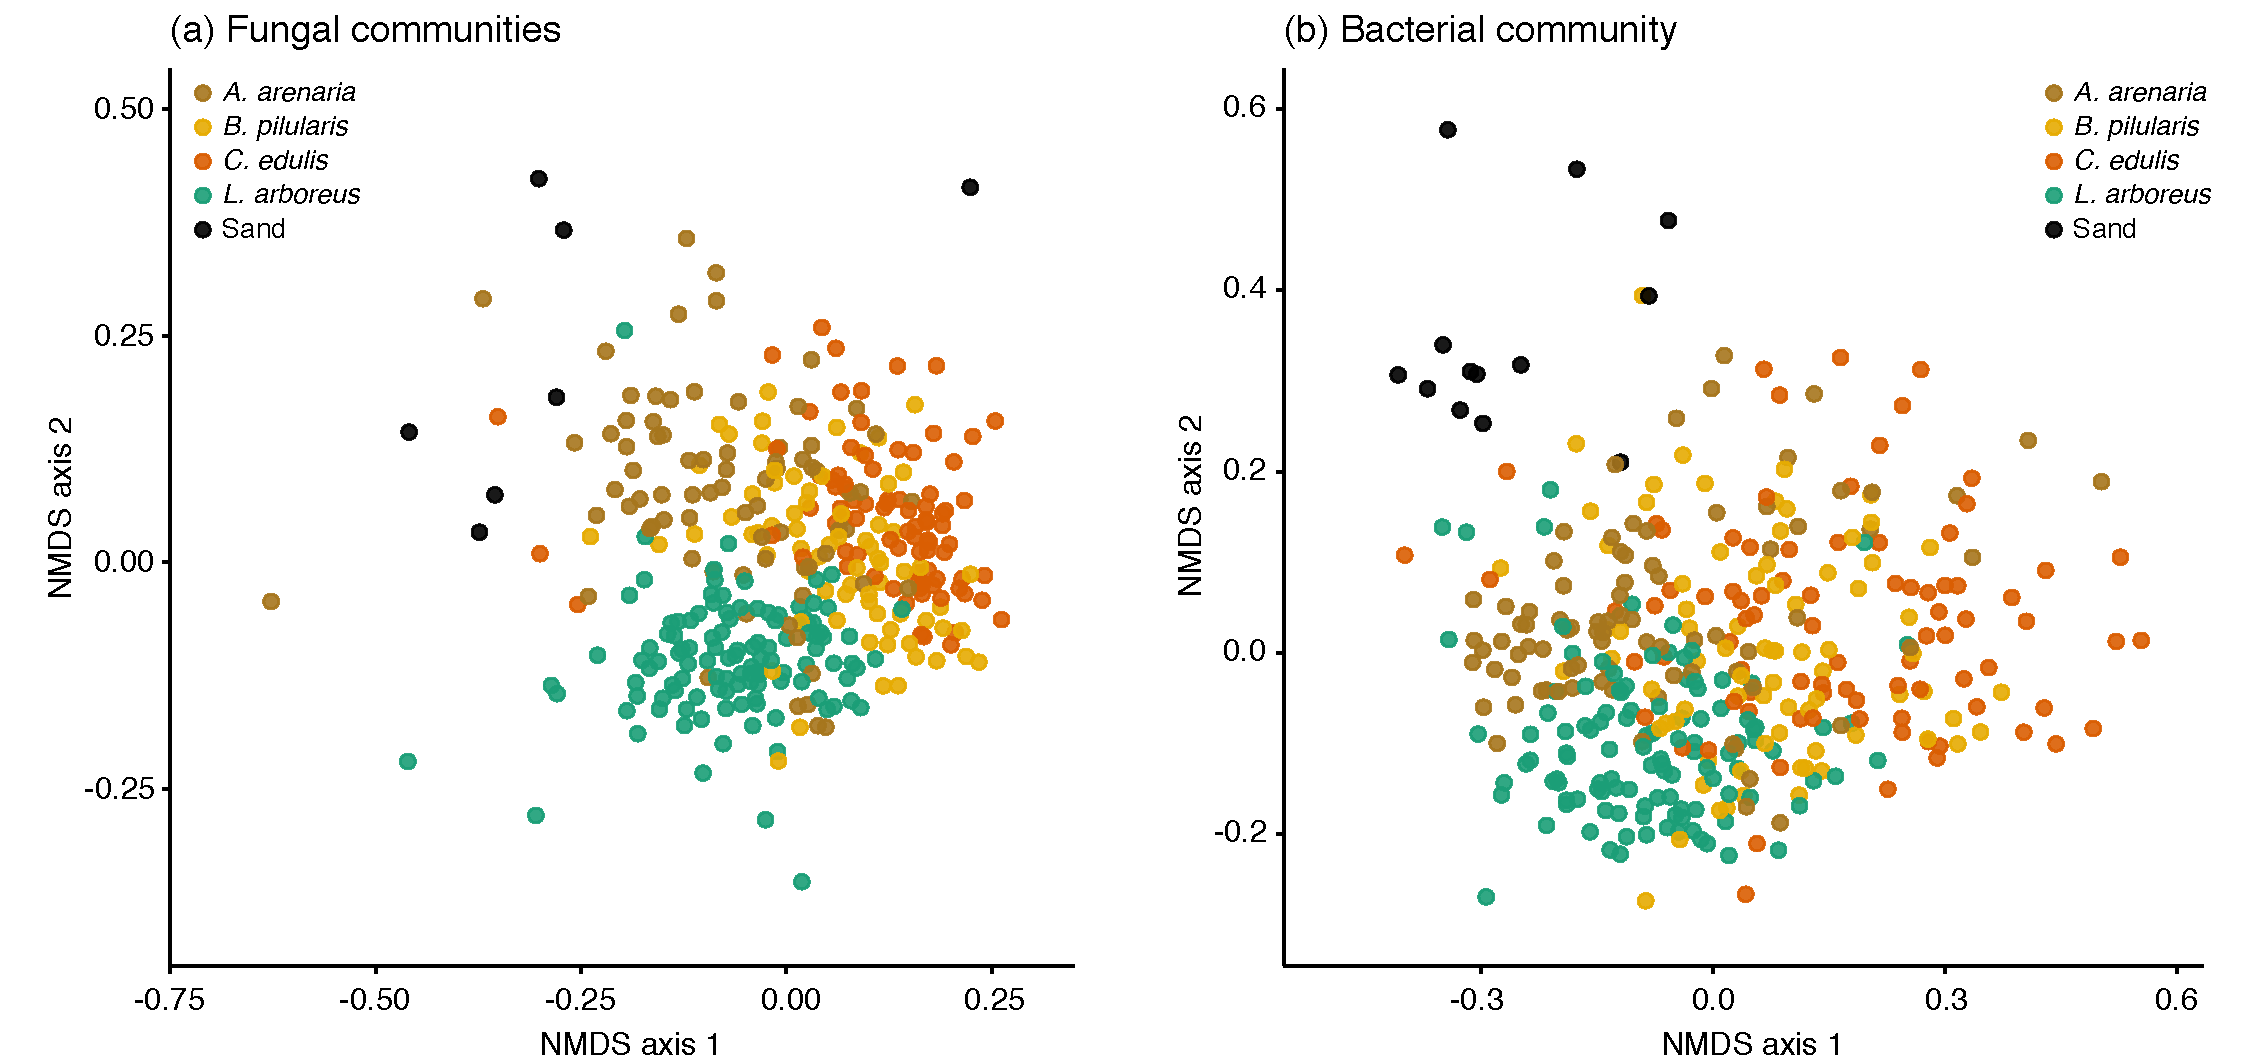
\includegraphics[width=17cm]{Chapter6/Composition_Both_Species.pdf}}
	\caption[NMDS ordination of all (a) fungal and (b) bacterial communities.]
		{\hspace{1mm} 
		NMDS ordination of all (a) fungal and (b) bacterial communities. Points are color-coded based on the identity of the plant species: \textit{A. arenaria} (brown); \textit{B. pilularis} (yellow); \textit{C. edulis} (orange); \textit{L. arboreus} (green); sand (black). 
		Statistics were performed at the plant individual level, but for visualization purpose each point represents the bacterial community of one soil sample. Panel (a) and (b) are the same ordination plot as in Figs \ref{fig:FunComposition} and \ref{fig:BacComposition}, respectively.}
	\label{fig:BothComposition}
\end{figure}



\newpage
\begin{figure}[h]
	\centering
	\makebox[\textwidth][c]{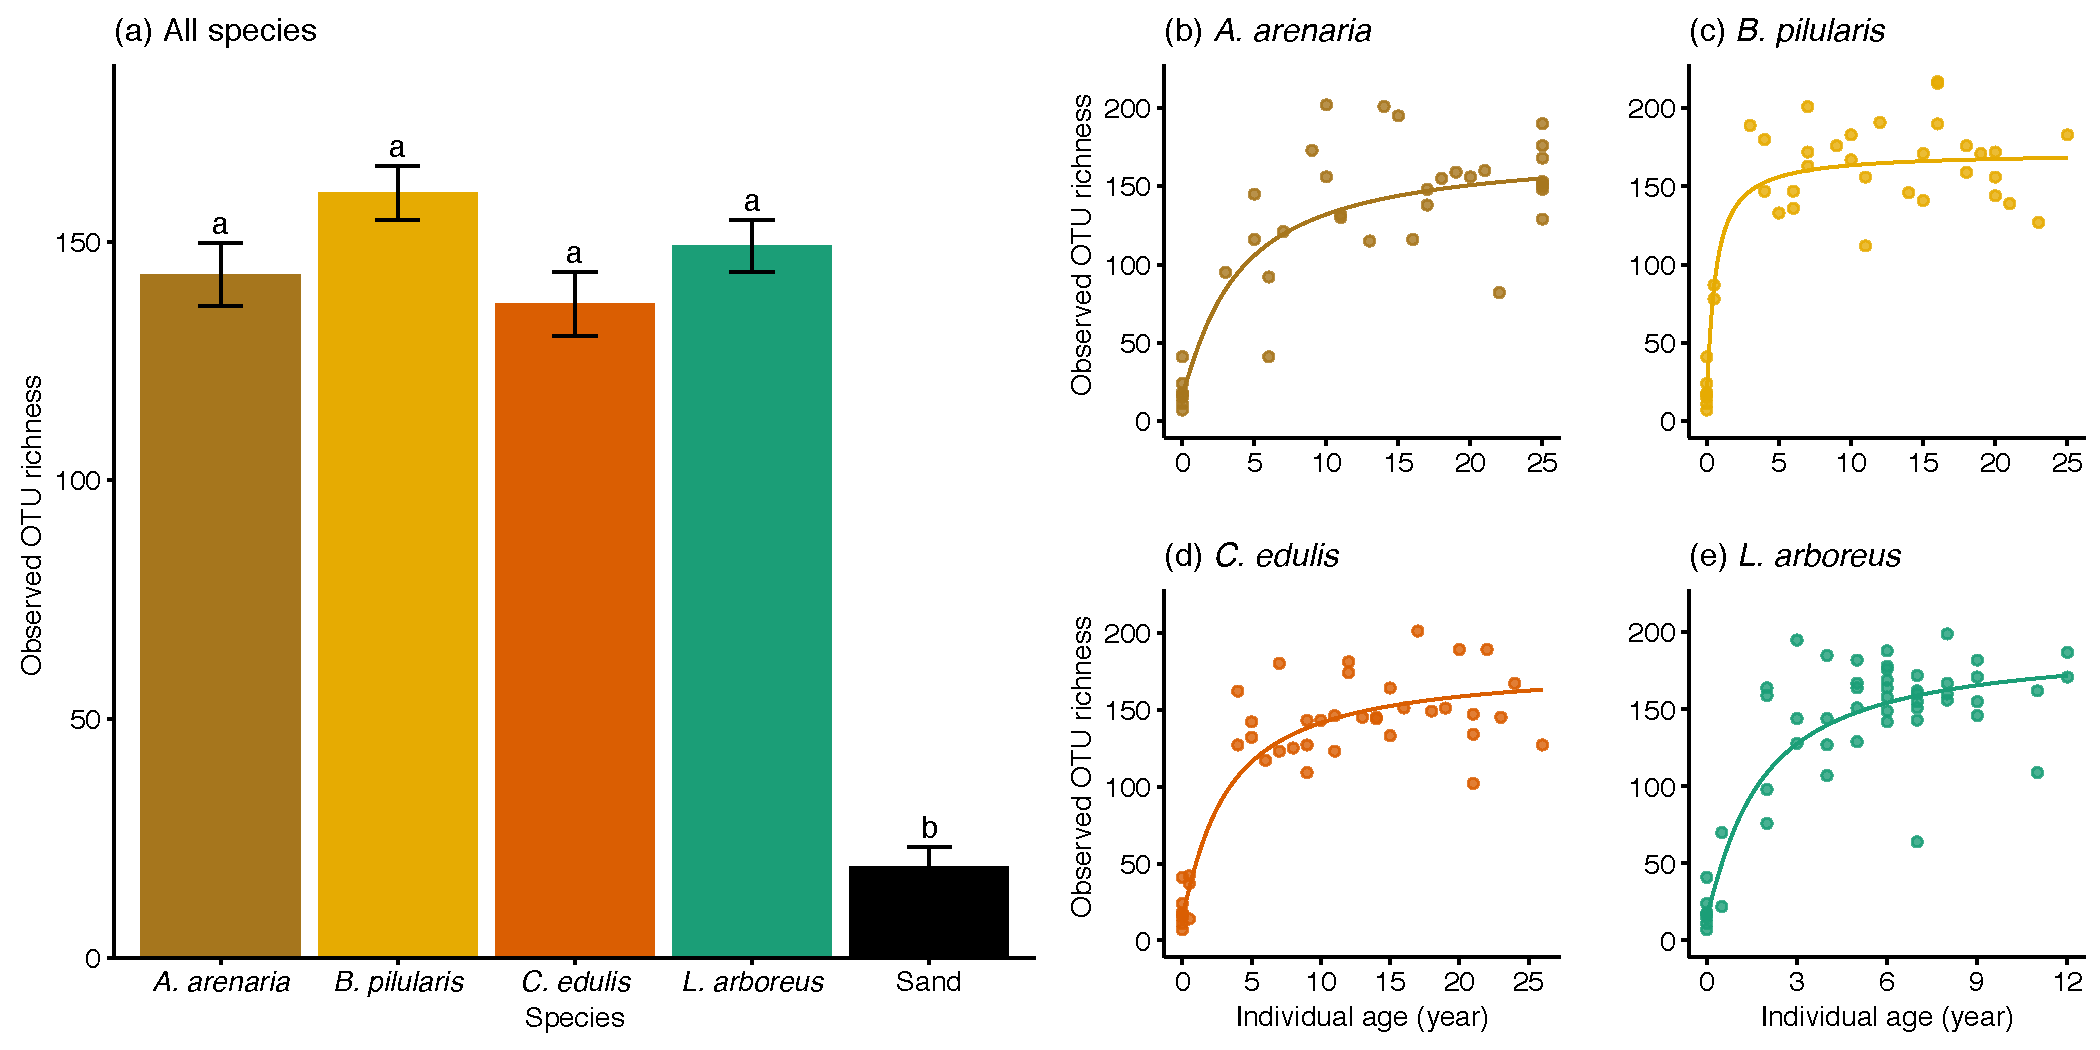
\includegraphics[width=17cm]{Chapter6/Richness_Fungi_Summary.pdf}}
	\caption[Fungal community richness as a function of plant age.]
		{\hspace{1mm} 
		Fungal community richness as a function of plant age. (a) Species-specific difference in observed fungal OTU richness. 
		(b)-(e) Temporal trend of observed richness with increasing plant age for each plant separately. (b) \textit{A. arenaria} (brown); (c) \textit{B. pilularis} (yellow); (d) \textit{C. edulis} (orange); (e) \textit{L. arboreus} (green). 
		Different letters in (a) represent significant difference among plant species. Each point in panels (b)-(e) represents the aggregated fungal community from one plant individual. A Monod function was the best fit for the temporal pattern: $\text{richness} = \mu \times \tfrac{\text{age}}{K + \text{age}} + m$, where $\mu$ is the maximum rate of richness increase, $K$ is the half-saturation constant, and $m$ is the minimum level offset.}
	\label{fig:FunRichness}
\end{figure}



\newpage
\begin{figure}[h]
	\centering
	\makebox[\textwidth][c]{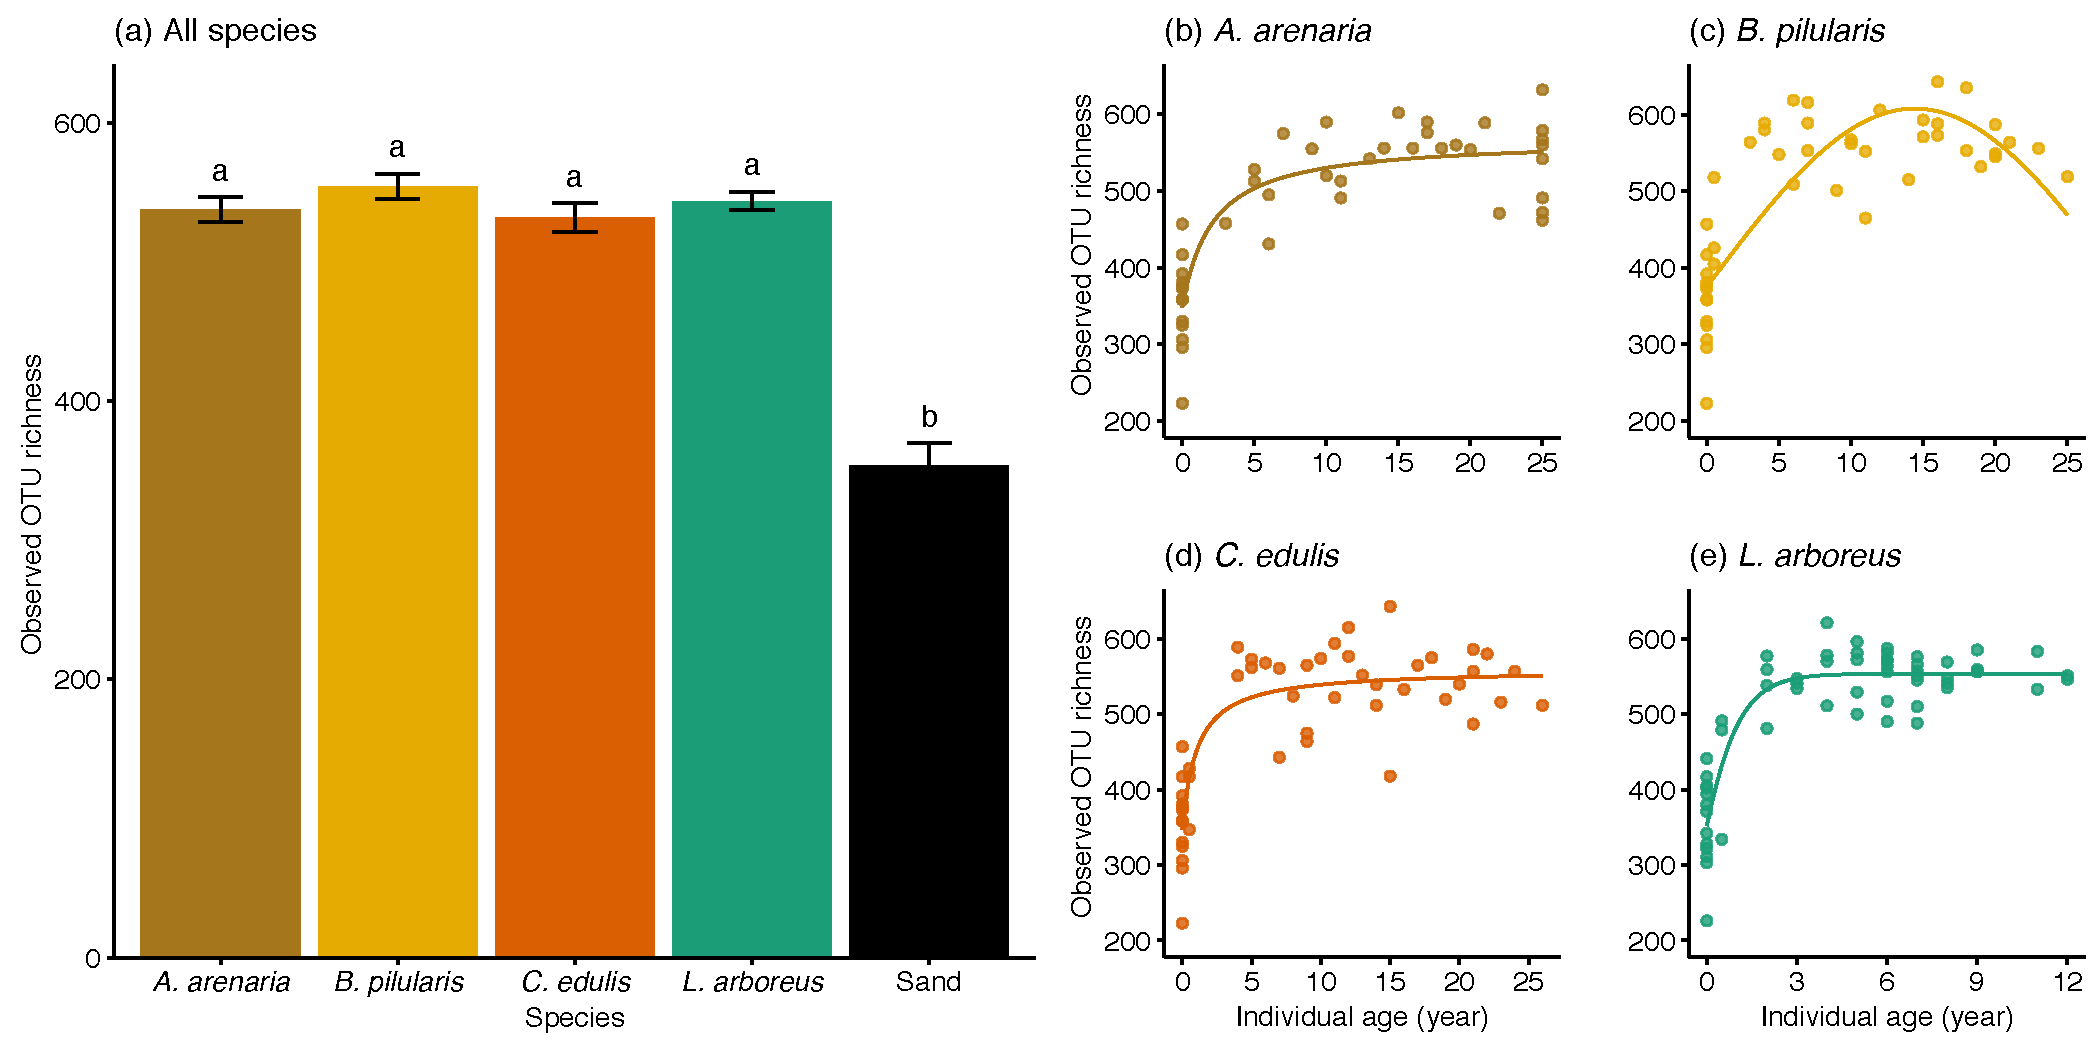
\includegraphics[width=17cm]{Chapter6/Richness_Bacteria_Summary.pdf}}
	\caption[Bacterial community richness as a function of plant age.]
		{\hspace{1mm} 
		Bacterial community richness as a function of plant age. (a) Species-specific difference in observed bacterial OTU richness.
		(b)-(e) Temporal trend of observed richness with increasing plant age for each plant separately. (b) \textit{A. arenaria} (brown); (c) \textit{B. pilularis} (yellow); (d) \textit{C. edulis} (orange); (e) \textit{L. arboreus} (green). 
		Different letters in (a) represent significant difference among plant species. Each point in panels (b)-(e) represents the aggregated bacterial  community from one plant individual. A quadratic function was the best fit for \textit{B. pilularis}, whereas a Monod function was the best fit for the other three species.}
	\label{fig:BacRichness}
\end{figure}



\newpage
\begin{figure}[h]
	\centering
	\makebox[\textwidth][c]{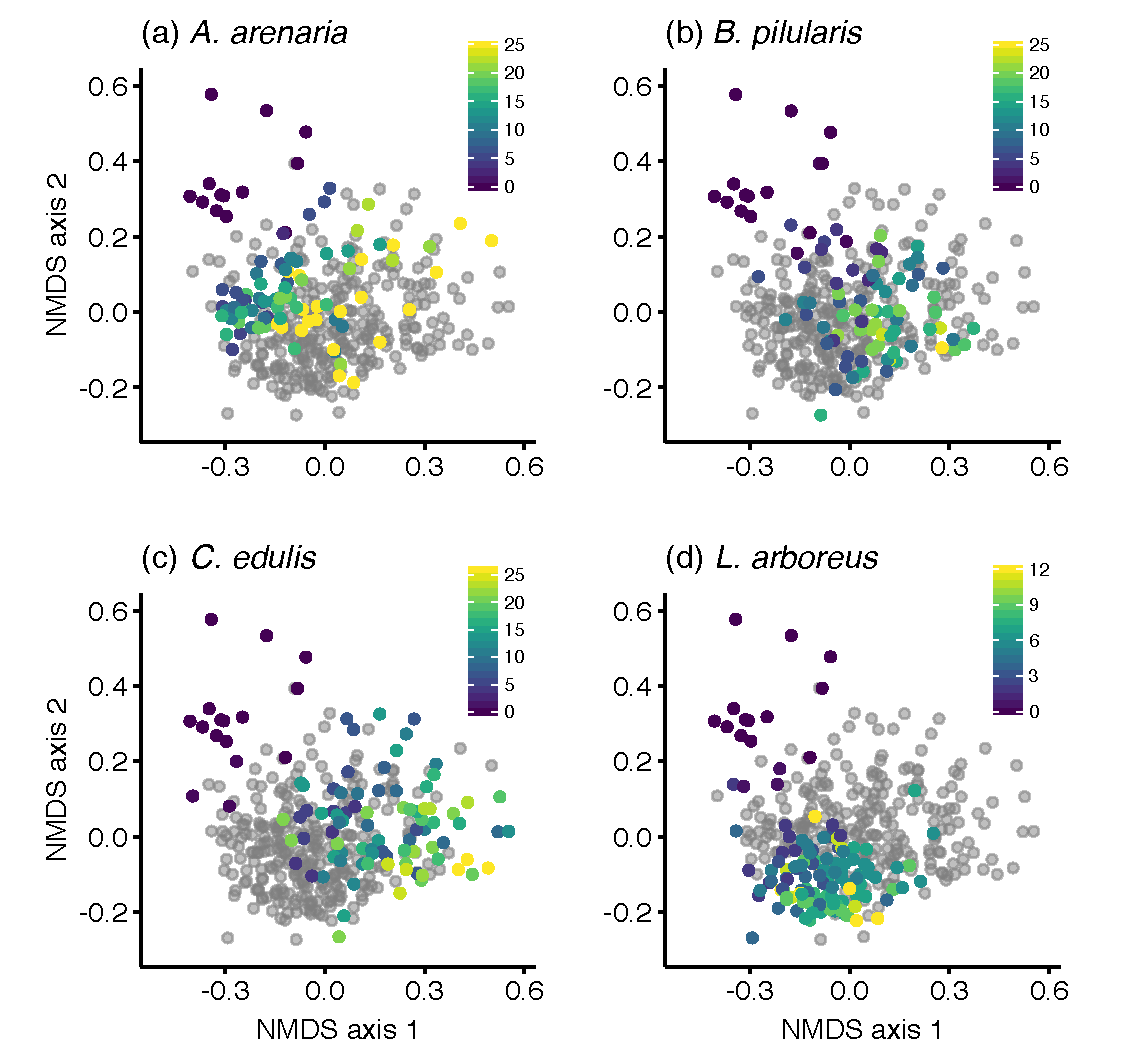
\includegraphics[width=13cm]{Chapter6/Composition_Bacteria_Age.pdf}}
	\caption[Bacterial community composition as a function of plant species and the age of plant individuals.]
		{\hspace{1mm} 
		Bacterial community composition as a function of plant species and the age of plant individuals. Each panel highlights one focal plant species on the NMDS ordination plot of all bacterial communities. Bacterial communities associated with the focal species are color-coded by individual plant age, whereas the other three species are in gray. Purple to yellow represent the age gradient from young to old, with species-specific minimum and maximum age. (a) \textit{A. arenaria}; (b) \textit{B. pilularis}; (c) \textit{C. edulis}; (d) \textit{L. arboreus}. 
		Statistics were performed at the plant individual level, but for visualization purpose each point represents the bacterial community of one soil sample. Note that dark purple points that appeared in all panels represent bacterial communities associated with bare sand. See the same ordination plot but color-coded with species identity in Fig.~\ref{fig:BothComposition}b.}
	\label{fig:BacComposition}
\end{figure}



\newpage
\begin{figure}[h]
	\centering
	\makebox[\textwidth][c]{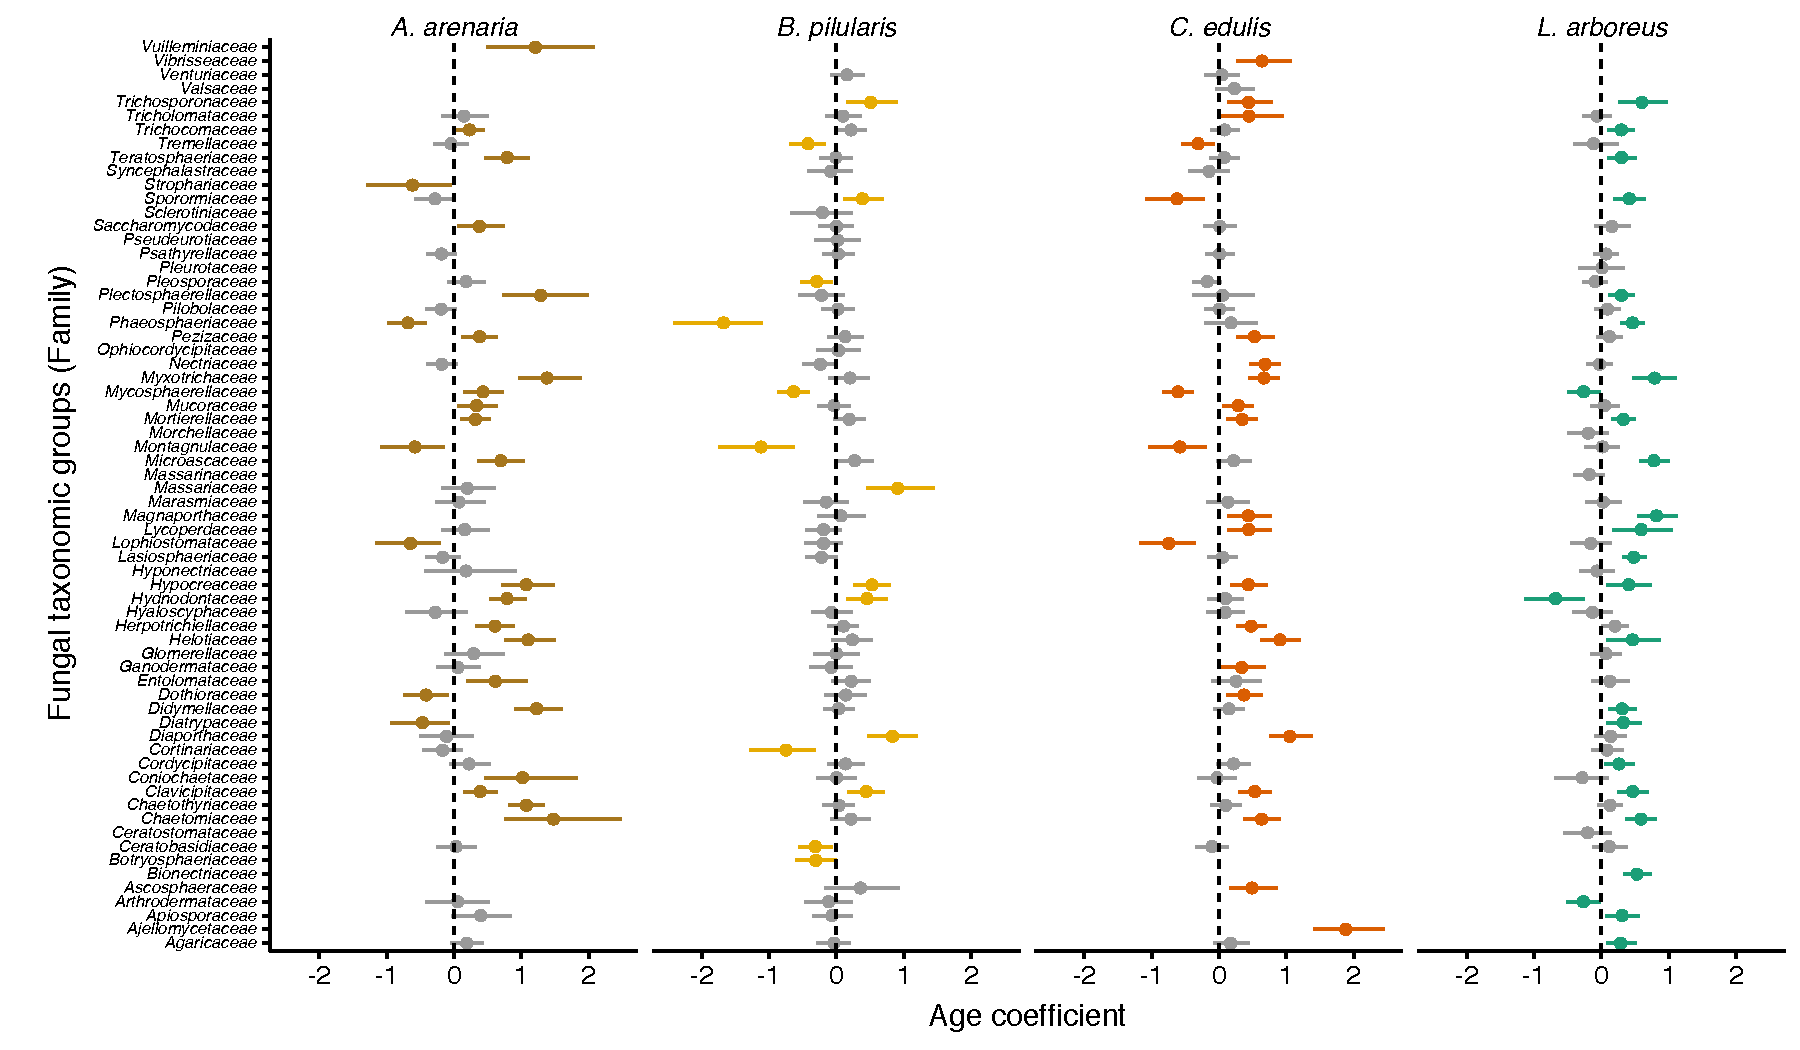
\includegraphics[width=18cm]{Chapter6/HMSC_Fungi_Family_Summary.pdf}}
	\caption[HMSC results demonstrating which fungal families show significant temporal trends.]
		{\hspace{1mm} HMSC results demonstrating which fungal families show significant temporal trends. Points and line segments represent the mean and the 95$\%$ credible interval of the fitted age coefficient for different fungal families (y-axis). All model fitting were performed separately for each plant species, from left to right: \textit{A. arenaria} (brown); \textit{B. pilularis} (yellow); \textit{C. edulis} (orange); \textit{L. arboreus} (green).}
	\label{fig:FunHMSC}
\end{figure}



\newpage
\begin{figure}[h]
	\centering
	\makebox[\textwidth][c]{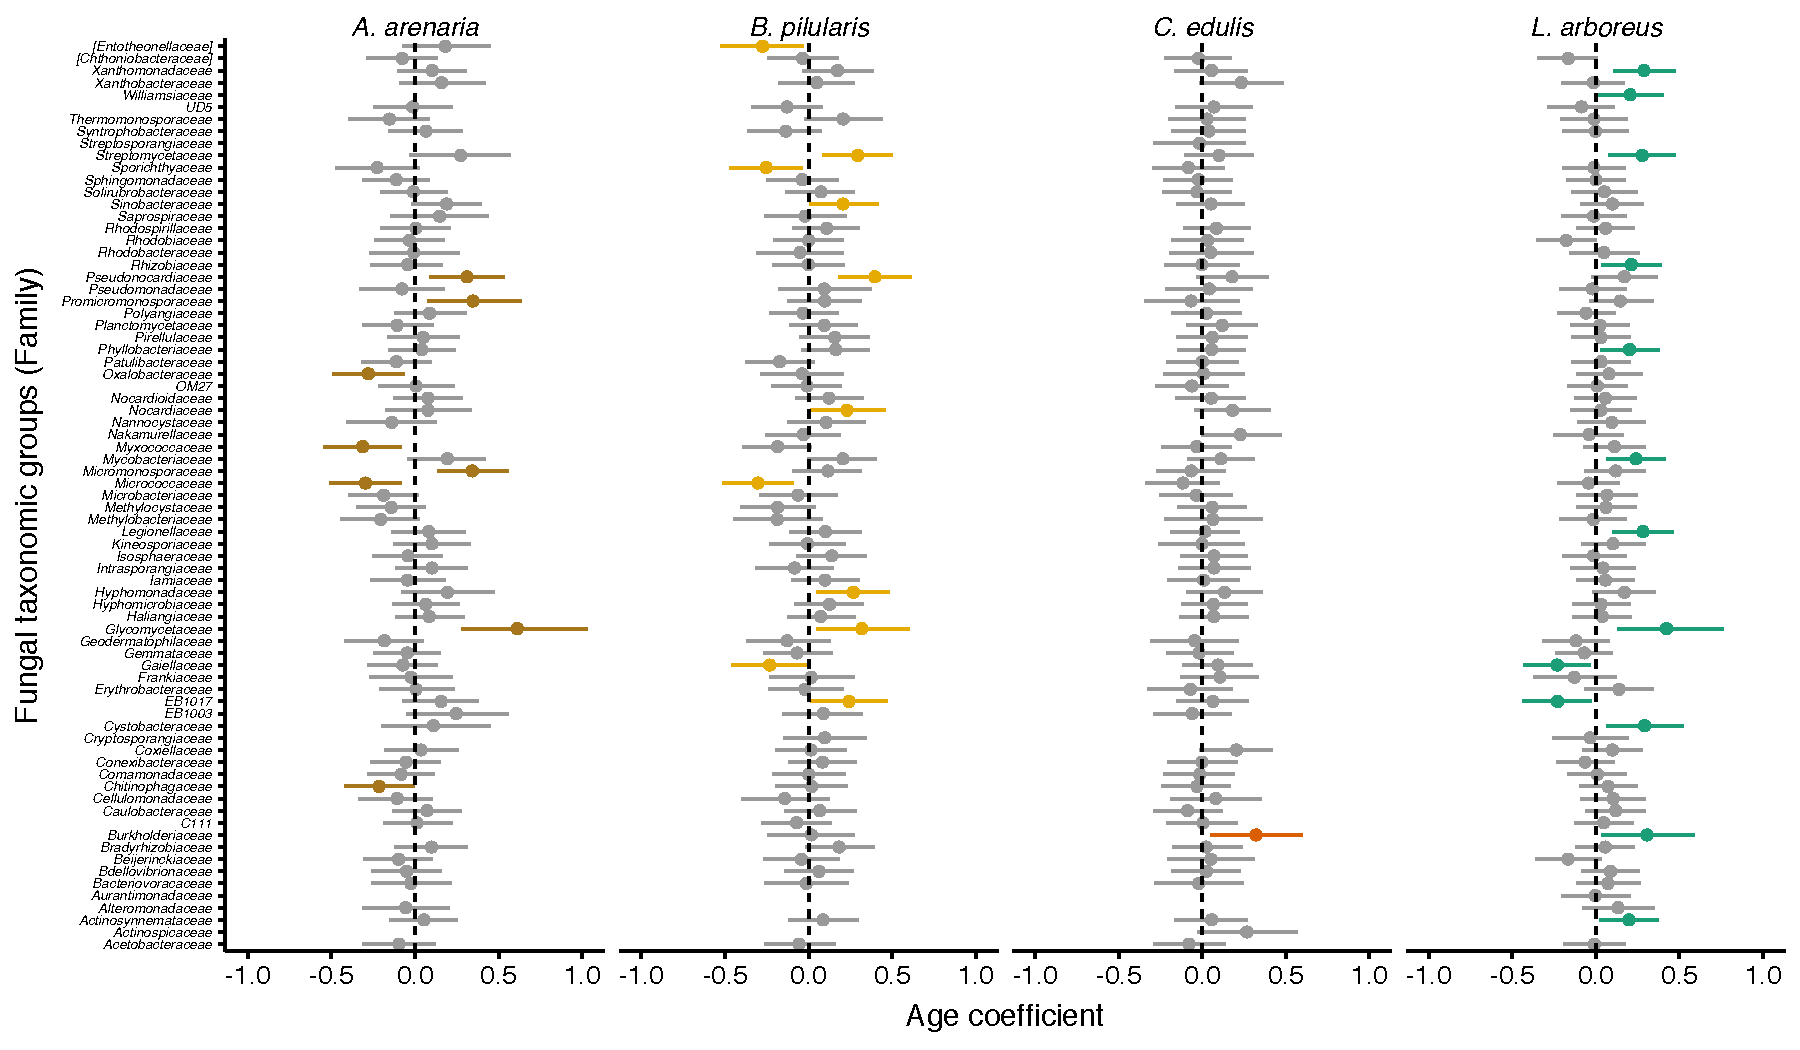
\includegraphics[width=18cm]{Chapter6/HMSC_Bacteria_Family_Summary.pdf}}
	\caption[HMSC results demonstrating which bacterial families show significant temporal trends.]
		{\hspace{1mm} HMSC results demonstrating which bacterial families show significant temporal trends. Points and line segments represent the mean and the 95$\%$ credible interval of the fitted age coefficient for different bacterial families (y-axis). All model fitting were performed separately for each plant species, from left to right: \textit{A. arenaria} (brown); \textit{B. pilularis} (yellow); \textit{C. edulis} (orange); \textit{L. arboreus} (green).}
	\label{fig:BacHMSC}
\end{figure}



\newpage
\begin{figure}[h]
	\centering
	\makebox[18cm][c]{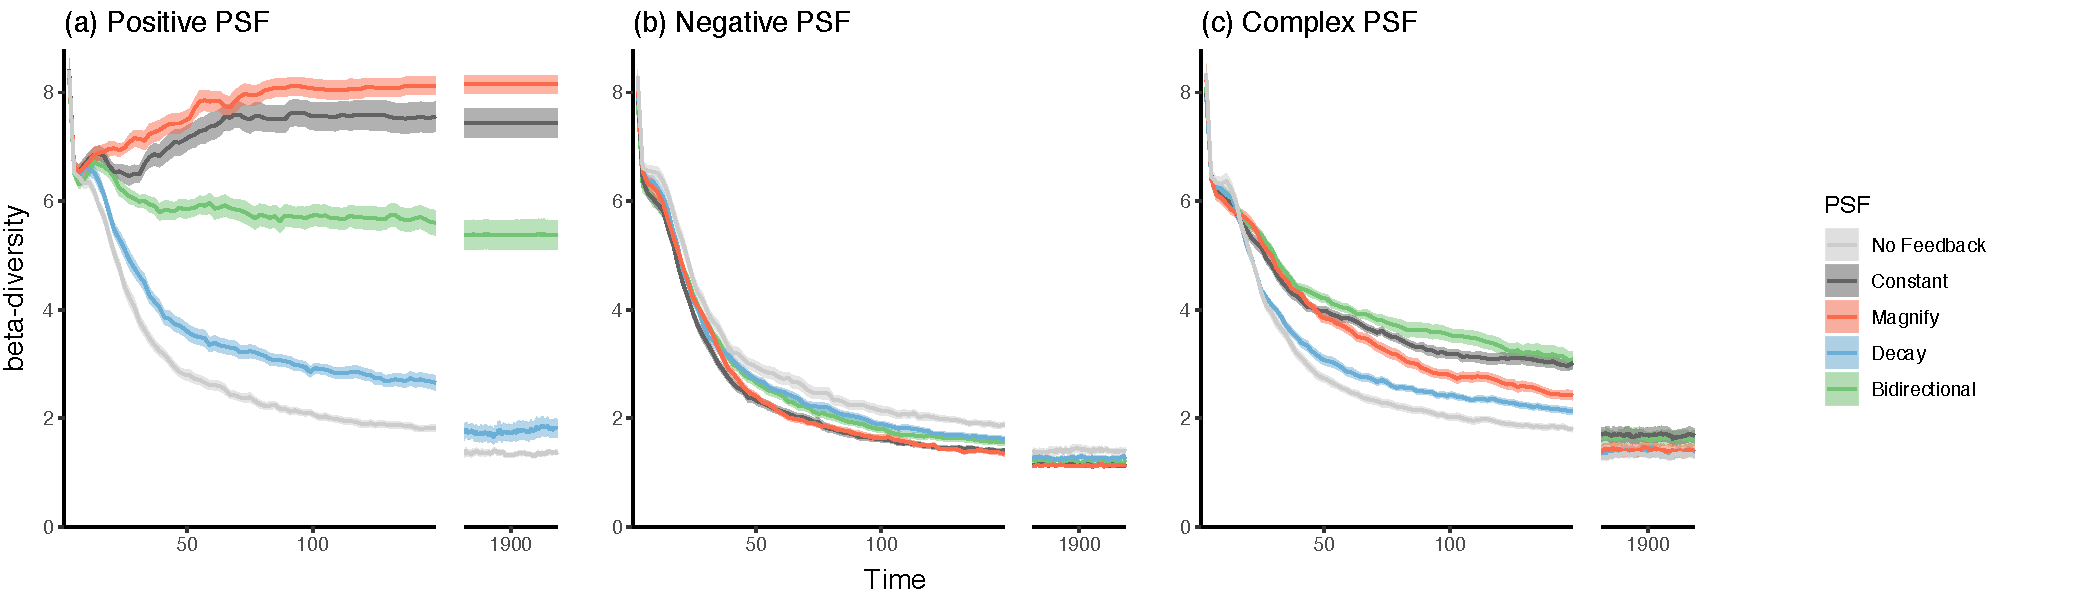
\includegraphics[width=18cm]{Chapter6/Simulation_AllPSF_Aggregate.pdf}}
	\caption[Simulated community convergence patterns under different plant--soil microbe interaction types and different temporal development scenarios.]
		{\hspace{1mm} 
		Simulated community convergence patterns under different plant--soil microbe interaction types and different temporal development scenarios.
		Each panel shows, under different plant--soil microbe interaction types, the temporal trends of beta-diversity (mean $\pm$ SE, $n = 20$) for different temporal development scenarios.
		(a) Positive conspecific plant--soil microbe interactions; (b) Negative conspecific plant--soil microbe interactions; (c) Complex plant--soil microbe interactions.
		Within each plant--soil microbe interaction type, the following temporal development scenarios were considered: 
		No plant--soil microbe interactions (light gray); Constant interaction strengths that are independent to plant age (black); Magnifying interaction strengths that intensify to their biological extremes with increasing plant age (orange); Decaying interaction strengths that attenuate to one with increasing plant age (blue); and Bidirectionally varying interaction strengths that either intensify or attenuate with increasing plant age (green). See Appendix S1 for detailed model description.}
	\label{fig:SimulationAllPSF}
\end{figure}





%% BIBLIOGRAPHY
\fancyhead[LE, RO]{\thepage}
\fancyhead[RE]{BIBLIOGRAPHY}
\fancyhead[LO]{BIBLIOGRAPHY}
\fancyfoot{}
\renewcommand{\headrulewidth}{0pt}
\bibliographystyle{ecol-mono}
\bibliography{ThesisBibliography}



\end{document}


